\documentclass[a4paper]{book}
\usepackage{a4wide}
\usepackage{makeidx}
\usepackage{fancyhdr}
\usepackage{graphicx}
\usepackage{multicol}
\usepackage{float}
\usepackage{textcomp}
\usepackage{alltt}
\usepackage{times}
\usepackage{ifpdf}
\ifpdf
\usepackage[pdftex,
            pagebackref=true,
            colorlinks=true,
            linkcolor=blue,
            unicode
           ]{hyperref}
\else
\usepackage[ps2pdf,
            pagebackref=true,
            colorlinks=true,
            linkcolor=blue,
            unicode
           ]{hyperref}
\usepackage{pspicture}
\fi
\usepackage[utf8]{inputenc}
\usepackage{doxygen}
\makeindex
\setcounter{tocdepth}{3}
\renewcommand{\footrulewidth}{0.4pt}
\begin{document}
\begin{titlepage}
\vspace*{7cm}
\begin{center}
{\Large Reference Manual}\\
\vspace*{1cm}
{\large Generated by Doxygen 1.5.8}\\
\vspace*{0.5cm}
{\small Wed Dec 1 20:38:58 2010}\\
\end{center}
\end{titlepage}
\clearemptydoublepage
\pagenumbering{roman}
\tableofcontents
\clearemptydoublepage
\pagenumbering{arabic}
\chapter{Class Index}
\section{Class Hierarchy}
This inheritance list is sorted roughly, but not completely, alphabetically:\begin{CompactList}
\item \contentsline{section}{StateHandler}{\pageref{classStateHandler}}{}
\begin{CompactList}
\item \contentsline{section}{AutoHoldStateHandler}{\pageref{classAutoHoldStateHandler}}{}
\item \contentsline{section}{ConnectedStateHandler}{\pageref{classConnectedStateHandler}}{}
\item \contentsline{section}{DialStateHandler}{\pageref{classDialStateHandler}}{}
\item \contentsline{section}{DisconnectStateHandler}{\pageref{classDisconnectStateHandler}}{}
\item \contentsline{section}{ExitStateHandler}{\pageref{classExitStateHandler}}{}
\item \contentsline{section}{HoldStateHandler}{\pageref{classHoldStateHandler}}{}
\item \contentsline{section}{MenuStateHandler}{\pageref{classMenuStateHandler}}{}
\item \contentsline{section}{RegisterStateHandler}{\pageref{classRegisterStateHandler}}{}
\end{CompactList}
\item \contentsline{section}{TeleKarma}{\pageref{classTeleKarma}}{}
\item \contentsline{section}{TelephonyIfc}{\pageref{classTelephonyIfc}}{}
\end{CompactList}

\chapter{Class Index}
\section{Class List}
Here are the classes, structs, unions and interfaces with brief descriptions:\begin{CompactList}
\item\contentsline{section}{\hyperlink{classAutoHoldStateHandler}{AutoHoldStateHandler} (This class is responsible for placing a connected call on detect human hold, including recording, muting mic, playing a wav loop, detecting a DTMF tone, alerting the user if a human is detected, monitoring call connection state, and restoring the connection and mic upon retrieval or human detection )}{\pageref{classAutoHoldStateHandler}}{}
\item\contentsline{section}{\hyperlink{classConnectedStateHandler}{ConnectedStateHandler} (This class is responsible for user options and connection state handling when in a normal call connection (as opposed to one of the hold modes) )}{\pageref{classConnectedStateHandler}}{}
\item\contentsline{section}{\hyperlink{classDialStateHandler}{DialStateHandler} (This class is responsible for obtaining a SIP number from the user, initiating dialing, and confirming success or failure of the connection )}{\pageref{classDialStateHandler}}{}
\item\contentsline{section}{\hyperlink{classDisconnectStateHandler}{DisconnectStateHandler} (This class is responsible for disconnecting a call )}{\pageref{classDisconnectStateHandler}}{}
\item\contentsline{section}{\hyperlink{classExitStateHandler}{ExitStateHandler} (This class does nothing )}{\pageref{classExitStateHandler}}{}
\item\contentsline{section}{\hyperlink{classHoldStateHandler}{HoldStateHandler} (This class is responsible for placing a connected call on standard hold, including recording, playing a wav loop, presenting user options, detecting user commands and responding those commands and connection state appropriately )}{\pageref{classHoldStateHandler}}{}
\item\contentsline{section}{\hyperlink{classMenuStateHandler}{MenuStateHandler} (This class is responsible for displaying the simple menu presenting 'call' or 'quit' options and responding to either command )}{\pageref{classMenuStateHandler}}{}
\item\contentsline{section}{\hyperlink{classRegisterStateHandler}{RegisterStateHandler} (This class is responsible for initializing telephony and registering the user with an SIP registrar, including gathering SIP account information from the user, initiating registration, and verifying successful registration )}{\pageref{classRegisterStateHandler}}{}
\item\contentsline{section}{\hyperlink{classStateHandler}{StateHandler} }{\pageref{classStateHandler}}{}
\item\contentsline{section}{\hyperlink{classTeleKarma}{TeleKarma} }{\pageref{classTeleKarma}}{}
\item\contentsline{section}{\hyperlink{classTelephonyIfc}{TelephonyIfc} (This class is the interface between telekarama and the Opal telephony library )}{\pageref{classTelephonyIfc}}{}
\end{CompactList}

\chapter{File Index}
\section{File List}
Here is a list of all files with brief descriptions:\begin{CompactList}
\item\contentsline{section}{\hyperlink{account_8cpp}{account.cpp} }{\pageref{account_8cpp}}{}
\item\contentsline{section}{\hyperlink{account_8h}{account.h} }{\pageref{account_8h}}{}
\item\contentsline{section}{\hyperlink{action_8cpp}{action.cpp} }{\pageref{action_8cpp}}{}
\item\contentsline{section}{\hyperlink{action_8h}{action.h} }{\pageref{action_8h}}{}
\item\contentsline{section}{\hyperlink{clicontext_8cpp}{clicontext.cpp} }{\pageref{clicontext_8cpp}}{}
\item\contentsline{section}{\hyperlink{clicontext_8h}{clicontext.h} }{\pageref{clicontext_8h}}{}
\item\contentsline{section}{\hyperlink{cliview_8cpp}{cliview.cpp} }{\pageref{cliview_8cpp}}{}
\item\contentsline{section}{\hyperlink{cliview_8h}{cliview.h} }{\pageref{cliview_8h}}{}
\item\contentsline{section}{\hyperlink{conf_8h}{conf.h} }{\pageref{conf_8h}}{}
\item\contentsline{section}{\hyperlink{controller_8cpp}{controller.cpp} }{\pageref{controller_8cpp}}{}
\item\contentsline{section}{\hyperlink{controller_8h}{controller.h} }{\pageref{controller_8h}}{}
\item\contentsline{section}{\hyperlink{gui_8cpp}{gui.cpp} }{\pageref{gui_8cpp}}{}
\item\contentsline{section}{\hyperlink{gui_8h}{gui.h} }{\pageref{gui_8h}}{}
\item\contentsline{section}{\hyperlink{main_8cpp}{main.cpp} }{\pageref{main_8cpp}}{}
\item\contentsline{section}{\hyperlink{model_8cpp}{model.cpp} }{\pageref{model_8cpp}}{}
\item\contentsline{section}{\hyperlink{model_8h}{model.h} }{\pageref{model_8h}}{}
\item\contentsline{section}{\hyperlink{pcss_8cpp}{pcss.cpp} }{\pageref{pcss_8cpp}}{}
\item\contentsline{section}{\hyperlink{pcss_8h}{pcss.h} }{\pageref{pcss_8h}}{}
\item\contentsline{section}{\hyperlink{sip_8cpp}{sip.cpp} }{\pageref{sip_8cpp}}{}
\item\contentsline{section}{\hyperlink{sip_8h}{sip.h} }{\pageref{sip_8h}}{}
\item\contentsline{section}{\hyperlink{state-new_8h}{state-new.h} }{\pageref{state-new_8h}}{}
\item\contentsline{section}{\hyperlink{state_8cpp}{state.cpp} }{\pageref{state_8cpp}}{}
\item\contentsline{section}{\hyperlink{state_8h}{state.h} }{\pageref{state_8h}}{}
\item\contentsline{section}{\hyperlink{telekarma_8cpp}{telekarma.cpp} }{\pageref{telekarma_8cpp}}{}
\item\contentsline{section}{\hyperlink{telekarma_8h}{telekarma.h} }{\pageref{telekarma_8h}}{}
\item\contentsline{section}{\hyperlink{telephony_8cpp}{telephony.cpp} }{\pageref{telephony_8cpp}}{}
\item\contentsline{section}{\hyperlink{telephony_8h}{telephony.h} }{\pageref{telephony_8h}}{}
\item\contentsline{section}{\hyperlink{view_8cpp}{view.cpp} }{\pageref{view_8cpp}}{}
\item\contentsline{section}{\hyperlink{view_8h}{view.h} }{\pageref{view_8h}}{}
\end{CompactList}

\chapter{Class Documentation}
\hypertarget{classAccount}{
\section{Account Class Reference}
\label{classAccount}\index{Account@{Account}}
}
Represents a user's account with a SIP service provider.  


{\tt \#include $<$account.h$>$}

\subsection*{Public Member Functions}
\begin{CompactItemize}
\item 
\hyperlink{classAccount_8f195affd9f203c7bec7970c4702768f}{Account} (const PString \&name, const PString \&registrar, const PString \&user)
\begin{CompactList}\small\item\em Construct an \hyperlink{classAccount}{Account} with a default STUN server. \item\end{CompactList}\item 
\hyperlink{classAccount_8325decb7b215b2860e3a4d7eaa72402}{Account} (const PString \&name, const PString \&registrar, const PString \&user, const PString \&stun)
\begin{CompactList}\small\item\em Construct an \hyperlink{classAccount}{Account} with user-specified STUN server. \item\end{CompactList}\item 
virtual \hyperlink{classAccount_569c9ef0e42b9157690b4ceb646daba8}{$\sim$Account} ()
\begin{CompactList}\small\item\em Destructor. \item\end{CompactList}\item 
const PString \& \hyperlink{classAccount_8e3cc9ed5f4f8bc36b68f352dd34af2c}{GetStunServer} () const 
\begin{CompactList}\small\item\em Returns the STUN server. \item\end{CompactList}\item 
const PString \& \hyperlink{classAccount_147ffe4f7db1e9f987af6a24927f638e}{GetRegistrar} () const 
\begin{CompactList}\small\item\em Returns the registrar. \item\end{CompactList}\item 
const PString \& \hyperlink{classAccount_3e372dec415f99fea4aef62356c451c4}{GetUser} () const 
\begin{CompactList}\small\item\em Returns the user (account) name. \item\end{CompactList}\item 
const PString \& \hyperlink{classAccount_9e97a246120c9a1b032dee5a1182f59d}{GetName} () const 
\begin{CompactList}\small\item\em Returns the account name. \item\end{CompactList}\item 
void \hyperlink{classAccount_28e1cfe654d233bb5eea03ae64e030dd}{SetStunServer} (const PString \&value)
\begin{CompactList}\small\item\em Sets the STUN server. \item\end{CompactList}\item 
void \hyperlink{classAccount_94f9db7a225897c903475c42425b28b1}{SetRegistrar} (const PString \&value)
\begin{CompactList}\small\item\em Sets the registrar. \item\end{CompactList}\item 
void \hyperlink{classAccount_796dd94d9e20801be1fe352fae44095f}{SetUser} (const PString \&value)
\begin{CompactList}\small\item\em Sets the user (account) name. \item\end{CompactList}\item 
void \hyperlink{classAccount_b4f94471843ffe5c49ef919b7a4c5dfe}{setName} (const PString \&value)
\begin{CompactList}\small\item\em Sets the account name. \item\end{CompactList}\end{CompactItemize}
\subsection*{Friends}
\begin{CompactItemize}
\item 
class \hyperlink{classAccount_37d0b1f5892301dabdceb70a7ec55ca3}{AccountList}
\end{CompactItemize}


\subsection{Detailed Description}
Represents a user's account with a SIP service provider. 

\subsection{Constructor \& Destructor Documentation}
\hypertarget{classAccount_8f195affd9f203c7bec7970c4702768f}{
\index{Account@{Account}!Account@{Account}}
\index{Account@{Account}!Account@{Account}}
\subsubsection[{Account}]{\setlength{\rightskip}{0pt plus 5cm}Account::Account (const PString \& {\em name}, \/  const PString \& {\em registrar}, \/  const PString \& {\em user})}}
\label{classAccount_8f195affd9f203c7bec7970c4702768f}


Construct an \hyperlink{classAccount}{Account} with a default STUN server. 

\hypertarget{classAccount_8325decb7b215b2860e3a4d7eaa72402}{
\index{Account@{Account}!Account@{Account}}
\index{Account@{Account}!Account@{Account}}
\subsubsection[{Account}]{\setlength{\rightskip}{0pt plus 5cm}Account::Account (const PString \& {\em name}, \/  const PString \& {\em registrar}, \/  const PString \& {\em user}, \/  const PString \& {\em stun})}}
\label{classAccount_8325decb7b215b2860e3a4d7eaa72402}


Construct an \hyperlink{classAccount}{Account} with user-specified STUN server. 

\hypertarget{classAccount_569c9ef0e42b9157690b4ceb646daba8}{
\index{Account@{Account}!$\sim$Account@{$\sim$Account}}
\index{$\sim$Account@{$\sim$Account}!Account@{Account}}
\subsubsection[{$\sim$Account}]{\setlength{\rightskip}{0pt plus 5cm}Account::$\sim$Account ()\hspace{0.3cm}{\tt  \mbox{[}virtual\mbox{]}}}}
\label{classAccount_569c9ef0e42b9157690b4ceb646daba8}


Destructor. 

Does nothing. 

\subsection{Member Function Documentation}
\hypertarget{classAccount_9e97a246120c9a1b032dee5a1182f59d}{
\index{Account@{Account}!GetName@{GetName}}
\index{GetName@{GetName}!Account@{Account}}
\subsubsection[{GetName}]{\setlength{\rightskip}{0pt plus 5cm}const PString \& Account::GetName () const}}
\label{classAccount_9e97a246120c9a1b032dee5a1182f59d}


Returns the account name. 

\hypertarget{classAccount_147ffe4f7db1e9f987af6a24927f638e}{
\index{Account@{Account}!GetRegistrar@{GetRegistrar}}
\index{GetRegistrar@{GetRegistrar}!Account@{Account}}
\subsubsection[{GetRegistrar}]{\setlength{\rightskip}{0pt plus 5cm}const PString \& Account::GetRegistrar () const}}
\label{classAccount_147ffe4f7db1e9f987af6a24927f638e}


Returns the registrar. 

\hypertarget{classAccount_8e3cc9ed5f4f8bc36b68f352dd34af2c}{
\index{Account@{Account}!GetStunServer@{GetStunServer}}
\index{GetStunServer@{GetStunServer}!Account@{Account}}
\subsubsection[{GetStunServer}]{\setlength{\rightskip}{0pt plus 5cm}const PString \& Account::GetStunServer () const}}
\label{classAccount_8e3cc9ed5f4f8bc36b68f352dd34af2c}


Returns the STUN server. 

\hypertarget{classAccount_3e372dec415f99fea4aef62356c451c4}{
\index{Account@{Account}!GetUser@{GetUser}}
\index{GetUser@{GetUser}!Account@{Account}}
\subsubsection[{GetUser}]{\setlength{\rightskip}{0pt plus 5cm}const PString \& Account::GetUser () const}}
\label{classAccount_3e372dec415f99fea4aef62356c451c4}


Returns the user (account) name. 

\hypertarget{classAccount_b4f94471843ffe5c49ef919b7a4c5dfe}{
\index{Account@{Account}!setName@{setName}}
\index{setName@{setName}!Account@{Account}}
\subsubsection[{setName}]{\setlength{\rightskip}{0pt plus 5cm}void Account::setName (const PString \& {\em value})}}
\label{classAccount_b4f94471843ffe5c49ef919b7a4c5dfe}


Sets the account name. 

\hypertarget{classAccount_94f9db7a225897c903475c42425b28b1}{
\index{Account@{Account}!SetRegistrar@{SetRegistrar}}
\index{SetRegistrar@{SetRegistrar}!Account@{Account}}
\subsubsection[{SetRegistrar}]{\setlength{\rightskip}{0pt plus 5cm}void Account::SetRegistrar (const PString \& {\em value})}}
\label{classAccount_94f9db7a225897c903475c42425b28b1}


Sets the registrar. 

\hypertarget{classAccount_28e1cfe654d233bb5eea03ae64e030dd}{
\index{Account@{Account}!SetStunServer@{SetStunServer}}
\index{SetStunServer@{SetStunServer}!Account@{Account}}
\subsubsection[{SetStunServer}]{\setlength{\rightskip}{0pt plus 5cm}void Account::SetStunServer (const PString \& {\em value})}}
\label{classAccount_28e1cfe654d233bb5eea03ae64e030dd}


Sets the STUN server. 

\hypertarget{classAccount_796dd94d9e20801be1fe352fae44095f}{
\index{Account@{Account}!SetUser@{SetUser}}
\index{SetUser@{SetUser}!Account@{Account}}
\subsubsection[{SetUser}]{\setlength{\rightskip}{0pt plus 5cm}void Account::SetUser (const PString \& {\em value})}}
\label{classAccount_796dd94d9e20801be1fe352fae44095f}


Sets the user (account) name. 



\subsection{Friends And Related Function Documentation}
\hypertarget{classAccount_37d0b1f5892301dabdceb70a7ec55ca3}{
\index{Account@{Account}!AccountList@{AccountList}}
\index{AccountList@{AccountList}!Account@{Account}}
\subsubsection[{AccountList}]{\setlength{\rightskip}{0pt plus 5cm}friend class {\bf AccountList}\hspace{0.3cm}{\tt  \mbox{[}friend\mbox{]}}}}
\label{classAccount_37d0b1f5892301dabdceb70a7ec55ca3}




The documentation for this class was generated from the following files:\begin{CompactItemize}
\item 
\hyperlink{account_8h}{account.h}\item 
\hyperlink{account_8cpp}{account.cpp}\end{CompactItemize}

\hypertarget{classAccountList}{
\section{AccountList Class Reference}
\label{classAccountList}\index{AccountList@{AccountList}}
}
Represents a persistant list of SIP service provider accounts.  


{\tt \#include $<$account.h$>$}

Collaboration diagram for AccountList:\nopagebreak
\begin{figure}[H]
\begin{center}
\leavevmode
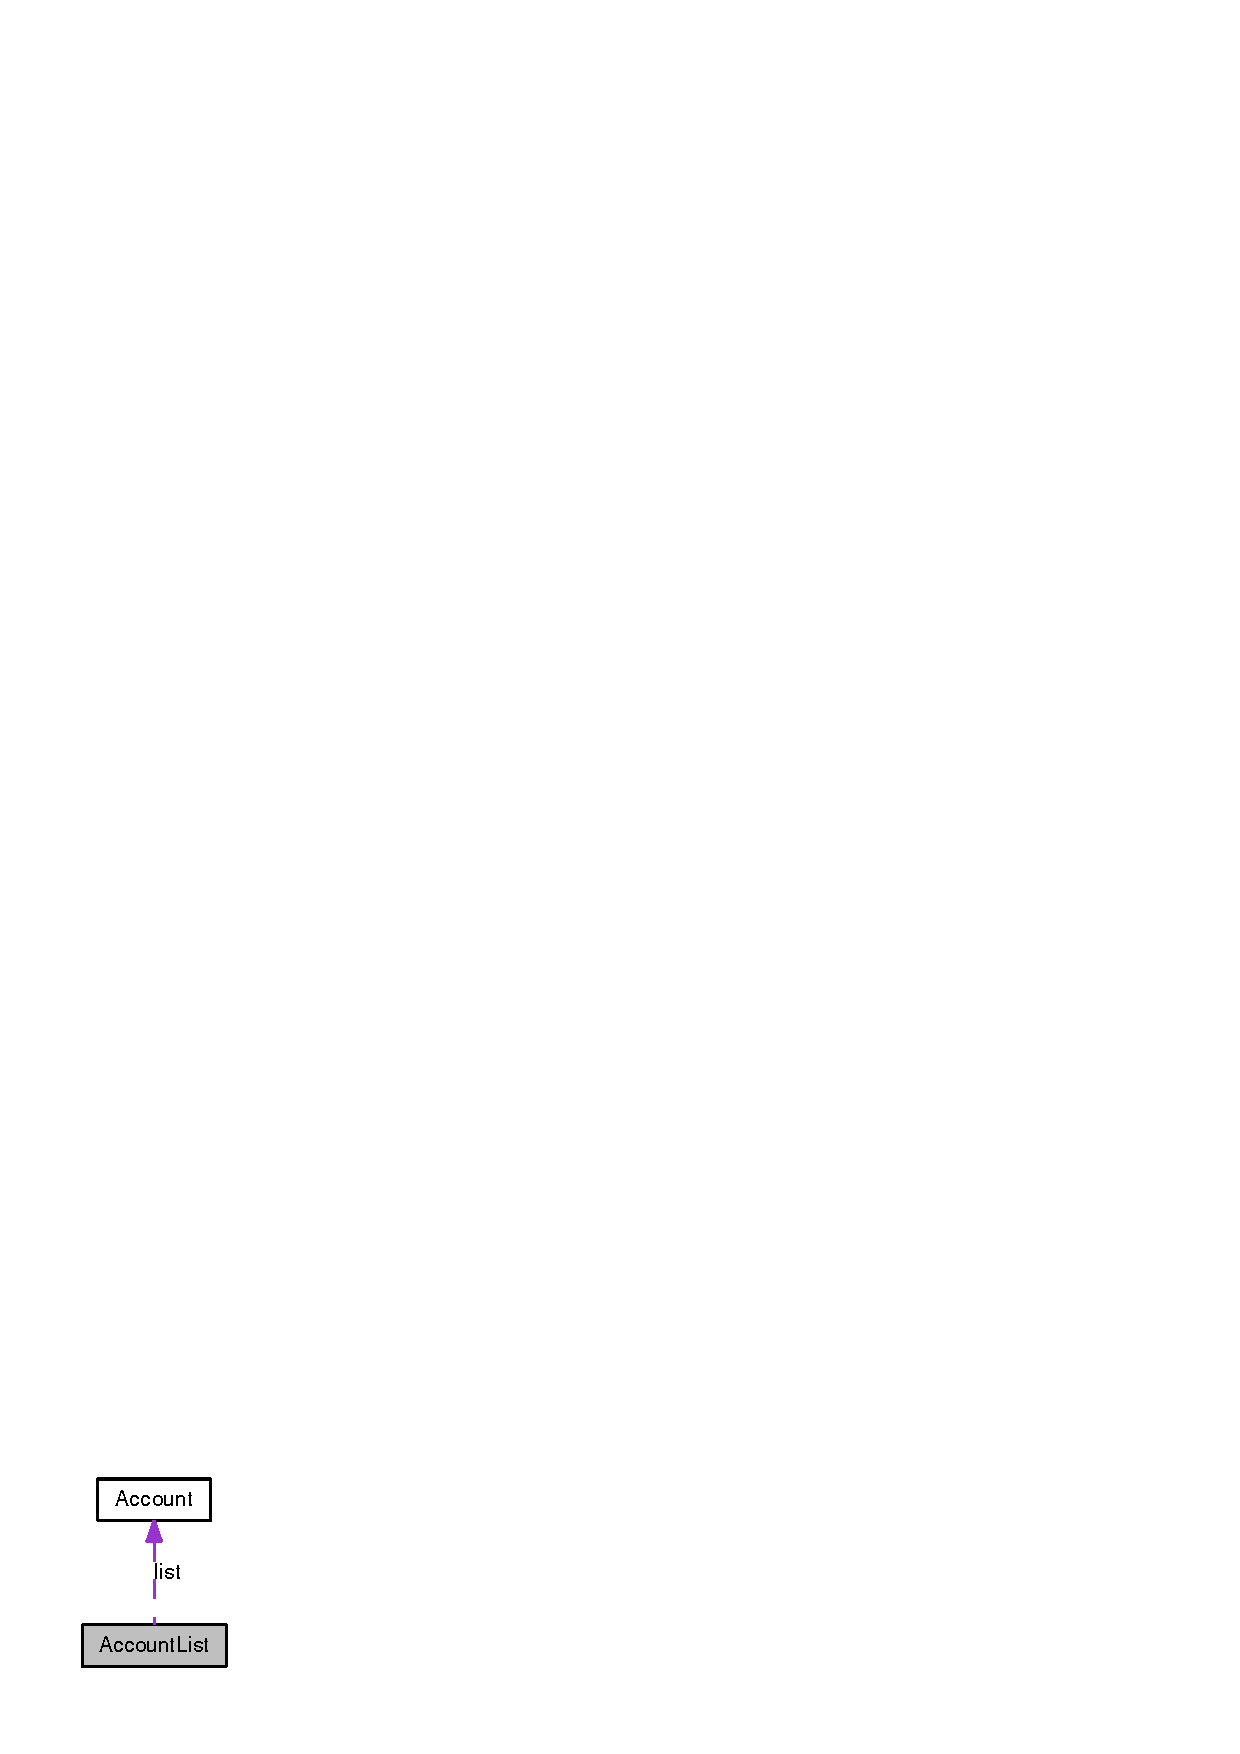
\includegraphics[width=112pt]{classAccountList__coll__graph}
\end{center}
\end{figure}
\subsection*{Public Member Functions}
\begin{CompactItemize}
\item 
\hyperlink{classAccountList_8e8092c5a958a03625dc9ff1915c8225}{AccountList} (const PString \&filename)
\begin{CompactList}\small\item\em Loads a new \hyperlink{classAccountList}{AccountList} from a file. \item\end{CompactList}\item 
virtual \hyperlink{classAccountList_77acd32be8700d21271e8802d87e2b15}{$\sim$AccountList} ()
\begin{CompactList}\small\item\em Deallocates all internal memory plus all \hyperlink{classAccount}{Account} objects. \item\end{CompactList}\item 
\hyperlink{classAccount}{Account} $\ast$ \hyperlink{classAccountList_c3d69942a3a661112f5a141bbbb80909}{GetAccount} (int index=0)
\begin{CompactList}\small\item\em Returns a pointer to an account in the list of accounts, or NULL if no such account exists. \item\end{CompactList}\item 
void \hyperlink{classAccountList_58880040232e0a6ba7e77096e26b6347}{AddAccount} (\hyperlink{classAccount}{Account} $\ast$account)
\begin{CompactList}\small\item\em Add a new account to this list. \item\end{CompactList}\item 
void \hyperlink{classAccountList_16a6b337fc14bce5ee4dd31f854592fc}{RemoveAccount} (const \hyperlink{classAccount}{Account} $\ast$account)
\begin{CompactList}\small\item\em Remove an account from the list. \item\end{CompactList}\item 
void \hyperlink{classAccountList_e94a2c11a78e44ac3724018d4142cbd7}{SetDefault} (const \hyperlink{classAccount}{Account} $\ast$account)
\begin{CompactList}\small\item\em Moves an account to the first array index. \item\end{CompactList}\item 
int \hyperlink{classAccountList_b83a124132b34cf82e5601609776daf9}{GetCount} () const 
\begin{CompactList}\small\item\em Returns the number of Accounts in the list. \item\end{CompactList}\item 
bool \hyperlink{classAccountList_f070ee0999c8406ed4c79ba4e131545a}{Save} () const 
\begin{CompactList}\small\item\em Saves the \hyperlink{classAccountList}{AccountList} to the file provided in the constructor. \item\end{CompactList}\item 
bool \hyperlink{classAccountList_1a289fad4cfa2e10362a3de84e2bd091}{SaveTo} (const PString \&filename) const 
\begin{CompactList}\small\item\em Saves the \hyperlink{classAccountList}{AccountList} to a file whose name is provided by the caller. \item\end{CompactList}\end{CompactItemize}


\subsection{Detailed Description}
Represents a persistant list of SIP service provider accounts. 

\subsection{Constructor \& Destructor Documentation}
\hypertarget{classAccountList_8e8092c5a958a03625dc9ff1915c8225}{
\index{AccountList@{AccountList}!AccountList@{AccountList}}
\index{AccountList@{AccountList}!AccountList@{AccountList}}
\subsubsection[{AccountList}]{\setlength{\rightskip}{0pt plus 5cm}AccountList::AccountList (const PString \& {\em filename})}}
\label{classAccountList_8e8092c5a958a03625dc9ff1915c8225}


Loads a new \hyperlink{classAccountList}{AccountList} from a file. 

If the file does not exist, the \hyperlink{classAccountList}{AccountList} will be empty. \hypertarget{classAccountList_77acd32be8700d21271e8802d87e2b15}{
\index{AccountList@{AccountList}!$\sim$AccountList@{$\sim$AccountList}}
\index{$\sim$AccountList@{$\sim$AccountList}!AccountList@{AccountList}}
\subsubsection[{$\sim$AccountList}]{\setlength{\rightskip}{0pt plus 5cm}AccountList::$\sim$AccountList ()\hspace{0.3cm}{\tt  \mbox{[}virtual\mbox{]}}}}
\label{classAccountList_77acd32be8700d21271e8802d87e2b15}


Deallocates all internal memory plus all \hyperlink{classAccount}{Account} objects. 

Note that deleting this object will render pointers returned by \hyperlink{classAccountList_c3d69942a3a661112f5a141bbbb80909}{GetAccount()} unusable, since that heap memory will be deallocated. 

\subsection{Member Function Documentation}
\hypertarget{classAccountList_58880040232e0a6ba7e77096e26b6347}{
\index{AccountList@{AccountList}!AddAccount@{AddAccount}}
\index{AddAccount@{AddAccount}!AccountList@{AccountList}}
\subsubsection[{AddAccount}]{\setlength{\rightskip}{0pt plus 5cm}void AccountList::AddAccount ({\bf Account} $\ast$ {\em account})}}
\label{classAccountList_58880040232e0a6ba7e77096e26b6347}


Add a new account to this list. 

Note that it is an error to add the same \hyperlink{classAccount}{Account} (the same heap memory space) to multiple \hyperlink{classAccountList}{AccountList} objects. This \hyperlink{classAccountList}{AccountList} will assume responsibility for managing the memory associated with the passed \hyperlink{classAccount}{Account}. It is an error for the caller to subsequently delete the heap memory allocated to the pointer passed into this method. \hypertarget{classAccountList_c3d69942a3a661112f5a141bbbb80909}{
\index{AccountList@{AccountList}!GetAccount@{GetAccount}}
\index{GetAccount@{GetAccount}!AccountList@{AccountList}}
\subsubsection[{GetAccount}]{\setlength{\rightskip}{0pt plus 5cm}{\bf Account} $\ast$ AccountList::GetAccount (int {\em index} = {\tt 0})}}
\label{classAccountList_c3d69942a3a661112f5a141bbbb80909}


Returns a pointer to an account in the list of accounts, or NULL if no such account exists. 

This class retains responsibility for memory management. Deleting the returned pointer is an error. However, modification of the \hyperlink{classAccount}{Account} is allowed and expected as the means of editing contents of the list in place. \begin{Desc}
\item[Parameters:]
\begin{description}
\item[{\em index}]optional; the array index of the account sought; zero is the default index. \end{description}
\end{Desc}
\begin{Desc}
\item[Returns:]requested account or NULL if the index is out of range. \end{Desc}
\hypertarget{classAccountList_b83a124132b34cf82e5601609776daf9}{
\index{AccountList@{AccountList}!GetCount@{GetCount}}
\index{GetCount@{GetCount}!AccountList@{AccountList}}
\subsubsection[{GetCount}]{\setlength{\rightskip}{0pt plus 5cm}int AccountList::GetCount () const}}
\label{classAccountList_b83a124132b34cf82e5601609776daf9}


Returns the number of Accounts in the list. 

\hypertarget{classAccountList_16a6b337fc14bce5ee4dd31f854592fc}{
\index{AccountList@{AccountList}!RemoveAccount@{RemoveAccount}}
\index{RemoveAccount@{RemoveAccount}!AccountList@{AccountList}}
\subsubsection[{RemoveAccount}]{\setlength{\rightskip}{0pt plus 5cm}void AccountList::RemoveAccount (const {\bf Account} $\ast$ {\em account})}}
\label{classAccountList_16a6b337fc14bce5ee4dd31f854592fc}


Remove an account from the list. 

Note that this Account's heap memory will be deallocated, and pointers to this account retrieved using \hyperlink{classAccountList_c3d69942a3a661112f5a141bbbb80909}{GetAccount()} and the pointer passed in via \hyperlink{classAccountList_58880040232e0a6ba7e77096e26b6347}{AddAccount(Account $\ast$)} (when applicable) will be left dangling. Also note that the parameter must appear in this list and must be managed only by this \hyperlink{classAccountList}{AccountList}. \hypertarget{classAccountList_f070ee0999c8406ed4c79ba4e131545a}{
\index{AccountList@{AccountList}!Save@{Save}}
\index{Save@{Save}!AccountList@{AccountList}}
\subsubsection[{Save}]{\setlength{\rightskip}{0pt plus 5cm}bool AccountList::Save () const}}
\label{classAccountList_f070ee0999c8406ed4c79ba4e131545a}


Saves the \hyperlink{classAccountList}{AccountList} to the file provided in the constructor. 

If that file does not exist, it will be created if possible. \begin{Desc}
\item[Returns:]if successful \end{Desc}
\hypertarget{classAccountList_1a289fad4cfa2e10362a3de84e2bd091}{
\index{AccountList@{AccountList}!SaveTo@{SaveTo}}
\index{SaveTo@{SaveTo}!AccountList@{AccountList}}
\subsubsection[{SaveTo}]{\setlength{\rightskip}{0pt plus 5cm}bool AccountList::SaveTo (const PString \& {\em filename}) const}}
\label{classAccountList_1a289fad4cfa2e10362a3de84e2bd091}


Saves the \hyperlink{classAccountList}{AccountList} to a file whose name is provided by the caller. 

If that file does not exist, it will be created if possible. Use to make a backup copy of the account config file. \begin{Desc}
\item[Returns:]if successful \end{Desc}
\hypertarget{classAccountList_e94a2c11a78e44ac3724018d4142cbd7}{
\index{AccountList@{AccountList}!SetDefault@{SetDefault}}
\index{SetDefault@{SetDefault}!AccountList@{AccountList}}
\subsubsection[{SetDefault}]{\setlength{\rightskip}{0pt plus 5cm}void AccountList::SetDefault (const {\bf Account} $\ast$ {\em account})}}
\label{classAccountList_e94a2c11a78e44ac3724018d4142cbd7}


Moves an account to the first array index. 

The parameter must exist in the list. 

The documentation for this class was generated from the following files:\begin{CompactItemize}
\item 
\hyperlink{account_8h}{account.h}\item 
\hyperlink{account_8cpp}{account.cpp}\end{CompactItemize}

\hypertarget{classAction}{
\section{Action Class Reference}
\label{classAction}\index{Action@{Action}}
}
{\tt \#include $<$action.h$>$}

Inheritance diagram for Action:\nopagebreak
\begin{figure}[H]
\begin{center}
\leavevmode

\includegraphics[height=400pt]{classAction__inherit__graph}
\end{center}
\end{figure}
\subsection*{Public Member Functions}
\begin{CompactItemize}
\item 
\hyperlink{classAction_357539603b99a849c72646d1f7eb85e4}{Action} (enum \hyperlink{action_8h_3664bc98cf666c3d88d23f3fd5d9251c}{ActionID} \hyperlink{classAction_65ceb856e427411fa4eb8001880d41a8}{id}, int \hyperlink{classAction_51e5d56a6aa4a037e90df19587a225c7}{turn})
\item 
virtual \hyperlink{classAction_bcf4c6358f53a666631ace11b325a7cd}{$\sim$Action} ()
\end{CompactItemize}
\subsection*{Public Attributes}
\begin{CompactItemize}
\item 
enum \hyperlink{action_8h_3664bc98cf666c3d88d23f3fd5d9251c}{ActionID} \hyperlink{classAction_65ceb856e427411fa4eb8001880d41a8}{id}
\item 
const int \hyperlink{classAction_51e5d56a6aa4a037e90df19587a225c7}{turn}
\end{CompactItemize}


\subsection{Constructor \& Destructor Documentation}
\hypertarget{classAction_357539603b99a849c72646d1f7eb85e4}{
\index{Action@{Action}!Action@{Action}}
\index{Action@{Action}!Action@{Action}}
\subsubsection[{Action}]{\setlength{\rightskip}{0pt plus 5cm}Action::Action (enum {\bf ActionID} {\em id}, \/  int {\em turn})\hspace{0.3cm}{\tt  \mbox{[}inline\mbox{]}}}}
\label{classAction_357539603b99a849c72646d1f7eb85e4}


\hypertarget{classAction_bcf4c6358f53a666631ace11b325a7cd}{
\index{Action@{Action}!$\sim$Action@{$\sim$Action}}
\index{$\sim$Action@{$\sim$Action}!Action@{Action}}
\subsubsection[{$\sim$Action}]{\setlength{\rightskip}{0pt plus 5cm}virtual Action::$\sim$Action ()\hspace{0.3cm}{\tt  \mbox{[}inline, virtual\mbox{]}}}}
\label{classAction_bcf4c6358f53a666631ace11b325a7cd}




\subsection{Member Data Documentation}
\hypertarget{classAction_65ceb856e427411fa4eb8001880d41a8}{
\index{Action@{Action}!id@{id}}
\index{id@{id}!Action@{Action}}
\subsubsection[{id}]{\setlength{\rightskip}{0pt plus 5cm}enum {\bf ActionID} {\bf Action::id}}}
\label{classAction_65ceb856e427411fa4eb8001880d41a8}


\hypertarget{classAction_51e5d56a6aa4a037e90df19587a225c7}{
\index{Action@{Action}!turn@{turn}}
\index{turn@{turn}!Action@{Action}}
\subsubsection[{turn}]{\setlength{\rightskip}{0pt plus 5cm}const int {\bf Action::turn}}}
\label{classAction_51e5d56a6aa4a037e90df19587a225c7}




The documentation for this class was generated from the following file:\begin{CompactItemize}
\item 
\hyperlink{action_8h}{action.h}\end{CompactItemize}

\hypertarget{classAutoHoldAction}{
\section{AutoHoldAction Class Reference}
\label{classAutoHoldAction}\index{AutoHoldAction@{AutoHoldAction}}
}
{\tt \#include $<$action.h$>$}

Inheritance diagram for AutoHoldAction:\nopagebreak
\begin{figure}[H]
\begin{center}
\leavevmode
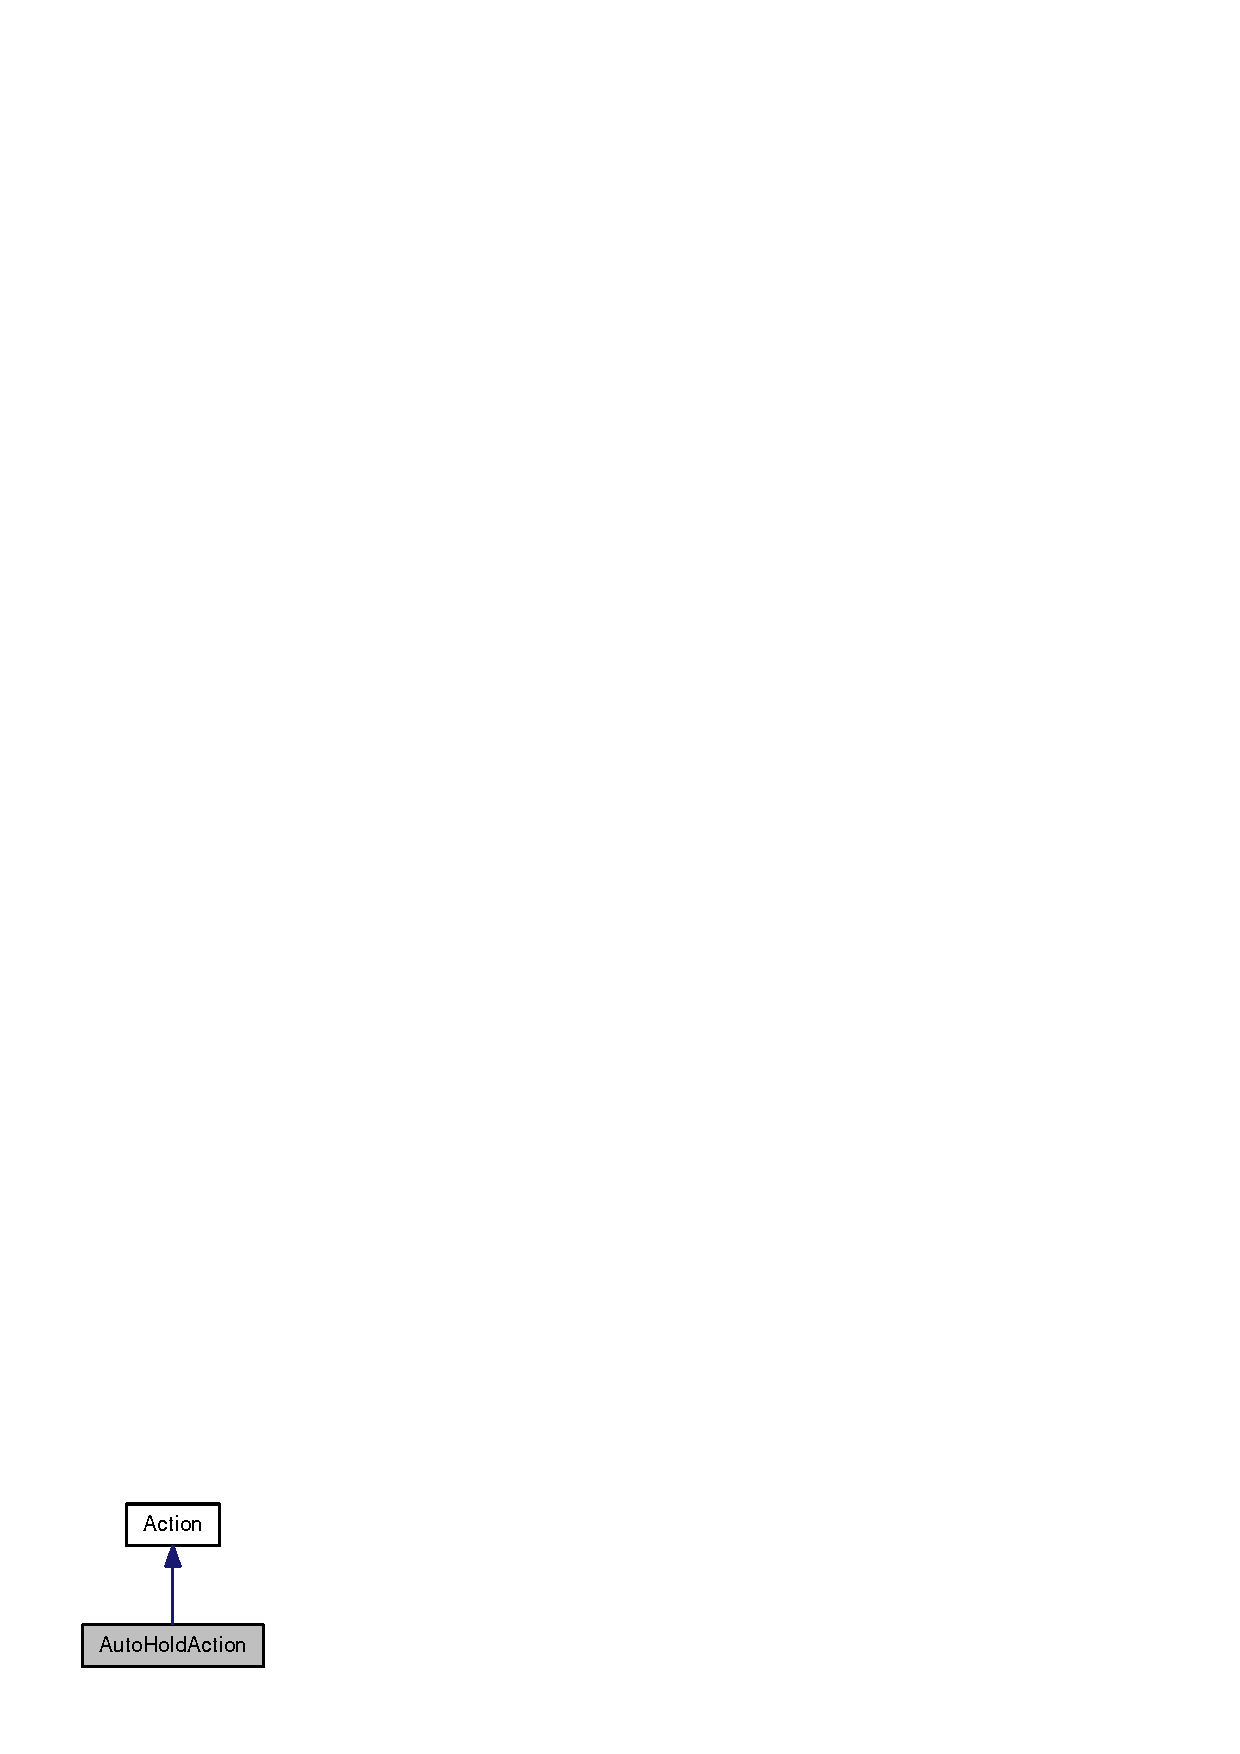
\includegraphics[width=130pt]{classAutoHoldAction__inherit__graph}
\end{center}
\end{figure}
Collaboration diagram for AutoHoldAction:\nopagebreak
\begin{figure}[H]
\begin{center}
\leavevmode

\includegraphics[width=130pt]{classAutoHoldAction__coll__graph}
\end{center}
\end{figure}
\subsection*{Public Member Functions}
\begin{CompactItemize}
\item 
\hyperlink{classAutoHoldAction_cff55ae9d07cf4e3b86569b78ebc07cc}{AutoHoldAction} (int \hyperlink{classAction_51e5d56a6aa4a037e90df19587a225c7}{turn})
\end{CompactItemize}


\subsection{Constructor \& Destructor Documentation}
\hypertarget{classAutoHoldAction_cff55ae9d07cf4e3b86569b78ebc07cc}{
\index{AutoHoldAction@{AutoHoldAction}!AutoHoldAction@{AutoHoldAction}}
\index{AutoHoldAction@{AutoHoldAction}!AutoHoldAction@{AutoHoldAction}}
\subsubsection[{AutoHoldAction}]{\setlength{\rightskip}{0pt plus 5cm}AutoHoldAction::AutoHoldAction (int {\em turn})\hspace{0.3cm}{\tt  \mbox{[}inline\mbox{]}}}}
\label{classAutoHoldAction_cff55ae9d07cf4e3b86569b78ebc07cc}




The documentation for this class was generated from the following file:\begin{CompactItemize}
\item 
\hyperlink{action_8h}{action.h}\end{CompactItemize}

\hypertarget{classCLIContext}{
\section{CLIContext Class Reference}
\label{classCLIContext}\index{CLIContext@{CLIContext}}
}
{\tt \#include $<$clicontext.h$>$}

\subsection*{Public Member Functions}
\begin{CompactItemize}
\item 
void \hyperlink{classCLIContext_c0bea8c8adbe7262b6e9a786ab691ed7}{OnCompletedLine} ()
\item 
bool \hyperlink{classCLIContext_4d8a44a878b5e5ebf767c55b7f872f63}{ProcessInput} (int ch)
\item 
bool \hyperlink{classCLIContext_f38452b224b03da39d12158922a90d19}{SetLocalEcho} (bool localEcho)
\item 
bool \hyperlink{classCLIContext_624d161af4a077a23c06d4e88254a787}{IsTouchTone} (PString line)
\end{CompactItemize}


\subsection{Member Function Documentation}
\hypertarget{classCLIContext_624d161af4a077a23c06d4e88254a787}{
\index{CLIContext@{CLIContext}!IsTouchTone@{IsTouchTone}}
\index{IsTouchTone@{IsTouchTone}!CLIContext@{CLIContext}}
\subsubsection[{IsTouchTone}]{\setlength{\rightskip}{0pt plus 5cm}bool CLIContext::IsTouchTone (PString {\em line})}}
\label{classCLIContext_624d161af4a077a23c06d4e88254a787}


\hypertarget{classCLIContext_c0bea8c8adbe7262b6e9a786ab691ed7}{
\index{CLIContext@{CLIContext}!OnCompletedLine@{OnCompletedLine}}
\index{OnCompletedLine@{OnCompletedLine}!CLIContext@{CLIContext}}
\subsubsection[{OnCompletedLine}]{\setlength{\rightskip}{0pt plus 5cm}void CLIContext::OnCompletedLine ()}}
\label{classCLIContext_c0bea8c8adbe7262b6e9a786ab691ed7}


\hypertarget{classCLIContext_4d8a44a878b5e5ebf767c55b7f872f63}{
\index{CLIContext@{CLIContext}!ProcessInput@{ProcessInput}}
\index{ProcessInput@{ProcessInput}!CLIContext@{CLIContext}}
\subsubsection[{ProcessInput}]{\setlength{\rightskip}{0pt plus 5cm}bool CLIContext::ProcessInput (int {\em ch})}}
\label{classCLIContext_4d8a44a878b5e5ebf767c55b7f872f63}


\hypertarget{classCLIContext_f38452b224b03da39d12158922a90d19}{
\index{CLIContext@{CLIContext}!SetLocalEcho@{SetLocalEcho}}
\index{SetLocalEcho@{SetLocalEcho}!CLIContext@{CLIContext}}
\subsubsection[{SetLocalEcho}]{\setlength{\rightskip}{0pt plus 5cm}bool CLIContext::SetLocalEcho (bool {\em localEcho})}}
\label{classCLIContext_f38452b224b03da39d12158922a90d19}




The documentation for this class was generated from the following files:\begin{CompactItemize}
\item 
\hyperlink{clicontext_8h}{clicontext.h}\item 
\hyperlink{clicontext_8cpp}{clicontext.cpp}\end{CompactItemize}

\hypertarget{classCLIView}{
\section{CLIView Class Reference}
\label{classCLIView}\index{CLIView@{CLIView}}
}
{\tt \#include $<$cliview.h$>$}

Inheritance diagram for CLIView:\nopagebreak
\begin{figure}[H]
\begin{center}
\leavevmode

\includegraphics[width=122pt]{classCLIView__inherit__graph}
\end{center}
\end{figure}
Collaboration diagram for CLIView:\nopagebreak
\begin{figure}[H]
\begin{center}
\leavevmode
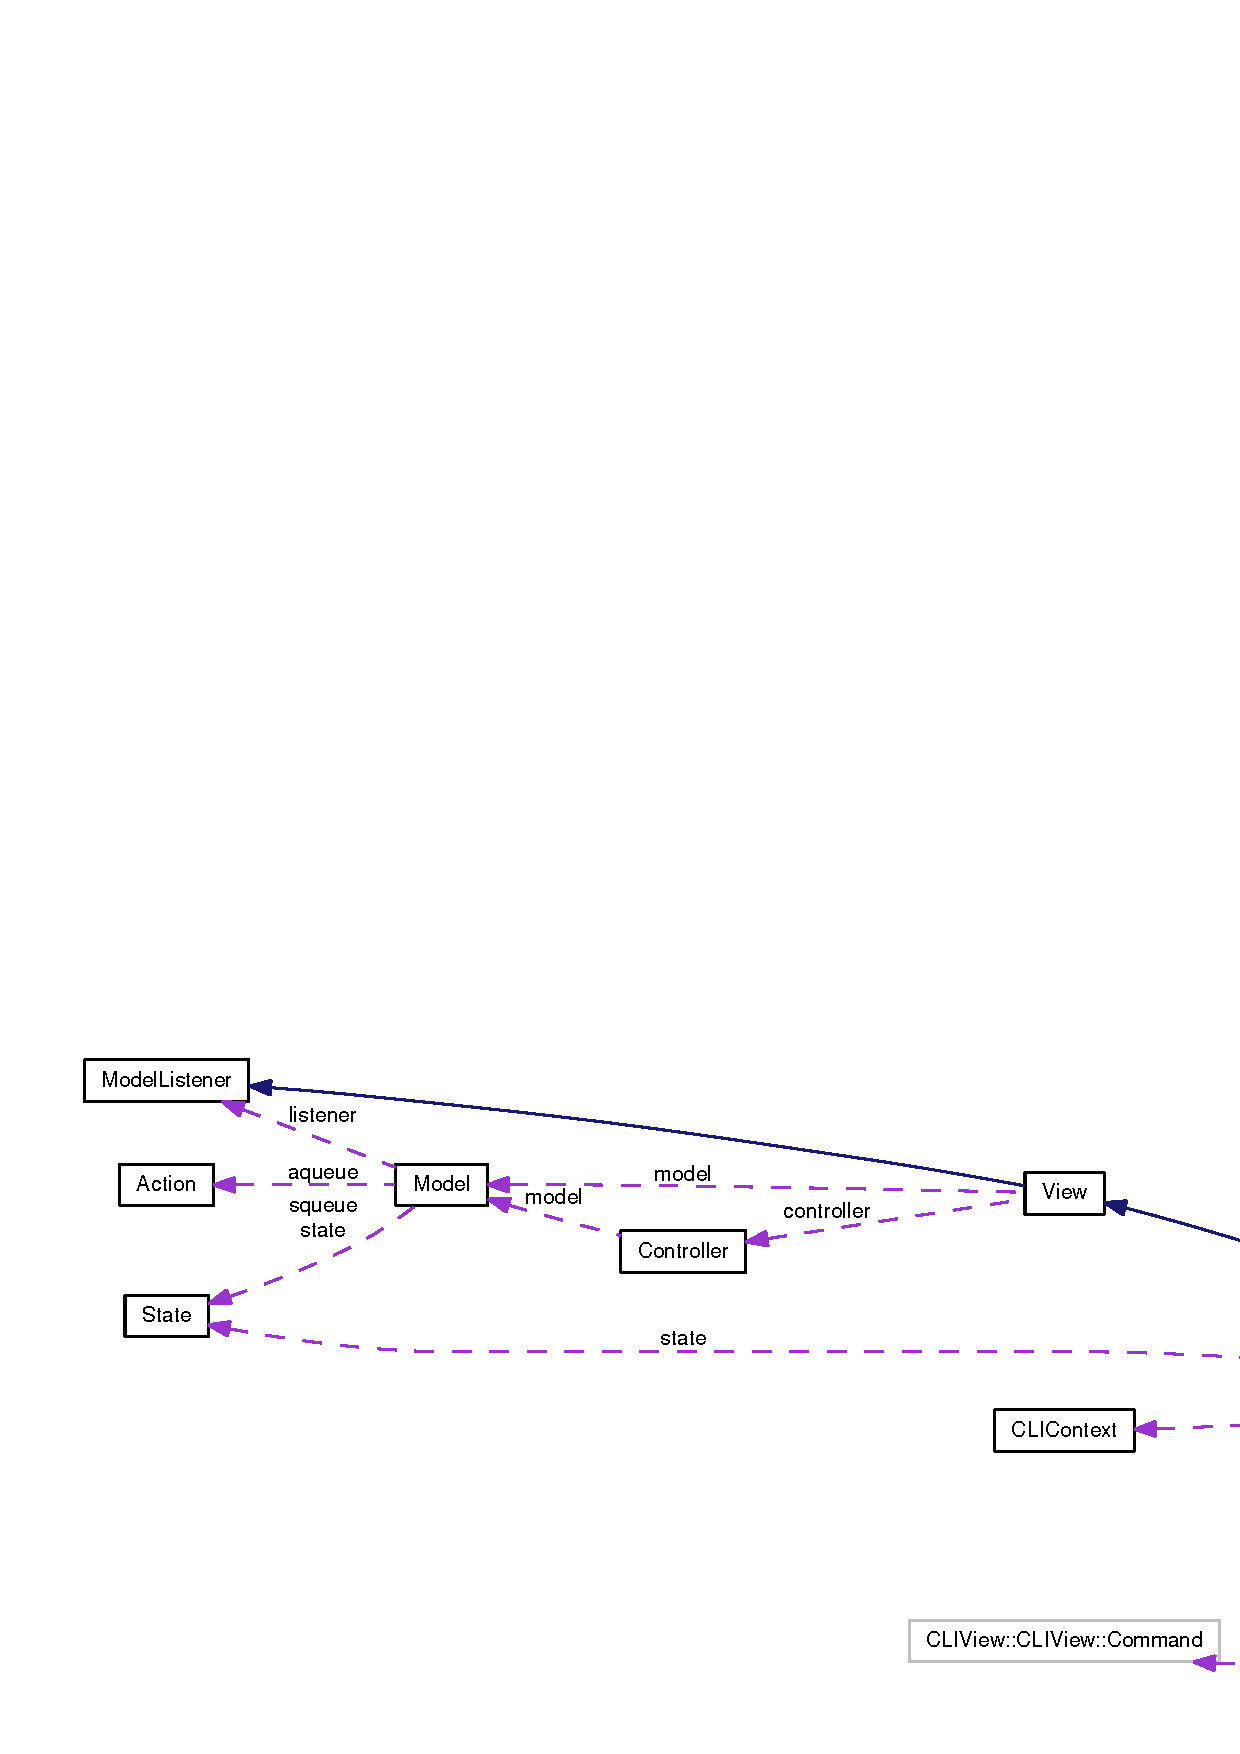
\includegraphics[width=400pt]{classCLIView__coll__graph}
\end{center}
\end{figure}
\subsection*{Classes}
\begin{CompactItemize}
\item 
class \textbf{Command}
\item 
class \textbf{DestInputHandler}
\item 
class \textbf{InputHandler}
\begin{CompactList}\small\item\em Parent class for all of the \hyperlink{classCLIView}{CLIView} input handlers. \item\end{CompactList}\item 
class \textbf{PasswordInputHandler}
\item 
class \textbf{RegistrarInputHandler}
\item 
class \textbf{STUNInputHandler}
\item 
class \textbf{UserInputHandler}
\end{CompactItemize}
\subsection*{Public Member Functions}
\begin{CompactItemize}
\item 
\hyperlink{classCLIView_53a3e66d584e90bb56f6e2266cbb5a6e}{CLIView} ()
\item 
\hyperlink{classCLIView_a2bfd6634095fd475ef131931aa8790c}{$\sim$CLIView} ()
\item 
void \hyperlink{classCLIView_e2c5d82a57753fee09f7fd20a14dd0db}{Main} ()
\end{CompactItemize}
\subsection*{Protected Member Functions}
\begin{CompactItemize}
\item 
PCLI::Context $\ast$ \hyperlink{classCLIView_56c18f1bd74cd25f293012457c7238eb}{CreateContext} ()
\end{CompactItemize}
\subsection*{Friends}
\begin{CompactItemize}
\item 
class \hyperlink{classCLIView_28c677eee06763681231ba62273b9fad}{InputHandler}
\item 
class \hyperlink{classCLIView_f9b3716dfe24382734846514b4626d04}{STUNInputHandler}
\item 
class \hyperlink{classCLIView_b160fef2c62aedd8169bf5670f1f291c}{RegistrarInputHandler}
\item 
class \hyperlink{classCLIView_17c53d72a733c0a2f0cc2103459d5aec}{UserInputHandler}
\item 
class \hyperlink{classCLIView_3351b3e1913bdd8c10a93b404ae26108}{PasswordInputHandler}
\item 
class \hyperlink{classCLIView_e9e28ac818dc78f00dff5c15398ff3ae}{DestInputHandler}
\end{CompactItemize}


\subsection{Constructor \& Destructor Documentation}
\hypertarget{classCLIView_53a3e66d584e90bb56f6e2266cbb5a6e}{
\index{CLIView@{CLIView}!CLIView@{CLIView}}
\index{CLIView@{CLIView}!CLIView@{CLIView}}
\subsubsection[{CLIView}]{\setlength{\rightskip}{0pt plus 5cm}CLIView::CLIView ()}}
\label{classCLIView_53a3e66d584e90bb56f6e2266cbb5a6e}


\hypertarget{classCLIView_a2bfd6634095fd475ef131931aa8790c}{
\index{CLIView@{CLIView}!$\sim$CLIView@{$\sim$CLIView}}
\index{$\sim$CLIView@{$\sim$CLIView}!CLIView@{CLIView}}
\subsubsection[{$\sim$CLIView}]{\setlength{\rightskip}{0pt plus 5cm}CLIView::$\sim$CLIView ()\hspace{0.3cm}{\tt  \mbox{[}inline\mbox{]}}}}
\label{classCLIView_a2bfd6634095fd475ef131931aa8790c}




\subsection{Member Function Documentation}
\hypertarget{classCLIView_56c18f1bd74cd25f293012457c7238eb}{
\index{CLIView@{CLIView}!CreateContext@{CreateContext}}
\index{CreateContext@{CreateContext}!CLIView@{CLIView}}
\subsubsection[{CreateContext}]{\setlength{\rightskip}{0pt plus 5cm}PCLI::Context $\ast$ CLIView::CreateContext ()\hspace{0.3cm}{\tt  \mbox{[}protected\mbox{]}}}}
\label{classCLIView_56c18f1bd74cd25f293012457c7238eb}


\hypertarget{classCLIView_e2c5d82a57753fee09f7fd20a14dd0db}{
\index{CLIView@{CLIView}!Main@{Main}}
\index{Main@{Main}!CLIView@{CLIView}}
\subsubsection[{Main}]{\setlength{\rightskip}{0pt plus 5cm}void CLIView::Main ()}}
\label{classCLIView_e2c5d82a57753fee09f7fd20a14dd0db}




\subsection{Friends And Related Function Documentation}
\hypertarget{classCLIView_e9e28ac818dc78f00dff5c15398ff3ae}{
\index{CLIView@{CLIView}!DestInputHandler@{DestInputHandler}}
\index{DestInputHandler@{DestInputHandler}!CLIView@{CLIView}}
\subsubsection[{DestInputHandler}]{\setlength{\rightskip}{0pt plus 5cm}friend class DestInputHandler\hspace{0.3cm}{\tt  \mbox{[}friend\mbox{]}}}}
\label{classCLIView_e9e28ac818dc78f00dff5c15398ff3ae}


\hypertarget{classCLIView_28c677eee06763681231ba62273b9fad}{
\index{CLIView@{CLIView}!InputHandler@{InputHandler}}
\index{InputHandler@{InputHandler}!CLIView@{CLIView}}
\subsubsection[{InputHandler}]{\setlength{\rightskip}{0pt plus 5cm}friend class InputHandler\hspace{0.3cm}{\tt  \mbox{[}friend\mbox{]}}}}
\label{classCLIView_28c677eee06763681231ba62273b9fad}


\hypertarget{classCLIView_3351b3e1913bdd8c10a93b404ae26108}{
\index{CLIView@{CLIView}!PasswordInputHandler@{PasswordInputHandler}}
\index{PasswordInputHandler@{PasswordInputHandler}!CLIView@{CLIView}}
\subsubsection[{PasswordInputHandler}]{\setlength{\rightskip}{0pt plus 5cm}friend class PasswordInputHandler\hspace{0.3cm}{\tt  \mbox{[}friend\mbox{]}}}}
\label{classCLIView_3351b3e1913bdd8c10a93b404ae26108}


\hypertarget{classCLIView_b160fef2c62aedd8169bf5670f1f291c}{
\index{CLIView@{CLIView}!RegistrarInputHandler@{RegistrarInputHandler}}
\index{RegistrarInputHandler@{RegistrarInputHandler}!CLIView@{CLIView}}
\subsubsection[{RegistrarInputHandler}]{\setlength{\rightskip}{0pt plus 5cm}friend class RegistrarInputHandler\hspace{0.3cm}{\tt  \mbox{[}friend\mbox{]}}}}
\label{classCLIView_b160fef2c62aedd8169bf5670f1f291c}


\hypertarget{classCLIView_f9b3716dfe24382734846514b4626d04}{
\index{CLIView@{CLIView}!STUNInputHandler@{STUNInputHandler}}
\index{STUNInputHandler@{STUNInputHandler}!CLIView@{CLIView}}
\subsubsection[{STUNInputHandler}]{\setlength{\rightskip}{0pt plus 5cm}friend class STUNInputHandler\hspace{0.3cm}{\tt  \mbox{[}friend\mbox{]}}}}
\label{classCLIView_f9b3716dfe24382734846514b4626d04}


\hypertarget{classCLIView_17c53d72a733c0a2f0cc2103459d5aec}{
\index{CLIView@{CLIView}!UserInputHandler@{UserInputHandler}}
\index{UserInputHandler@{UserInputHandler}!CLIView@{CLIView}}
\subsubsection[{UserInputHandler}]{\setlength{\rightskip}{0pt plus 5cm}friend class UserInputHandler\hspace{0.3cm}{\tt  \mbox{[}friend\mbox{]}}}}
\label{classCLIView_17c53d72a733c0a2f0cc2103459d5aec}




The documentation for this class was generated from the following files:\begin{CompactItemize}
\item 
\hyperlink{cliview_8h}{cliview.h}\item 
\hyperlink{cliview_8cpp}{cliview.cpp}\end{CompactItemize}

\hypertarget{classController}{
\section{Controller Class Reference}
\label{classController}\index{Controller@{Controller}}
}
{\tt \#include $<$controller.h$>$}

Inheritance diagram for Controller:\nopagebreak
\begin{figure}[H]
\begin{center}
\leavevmode
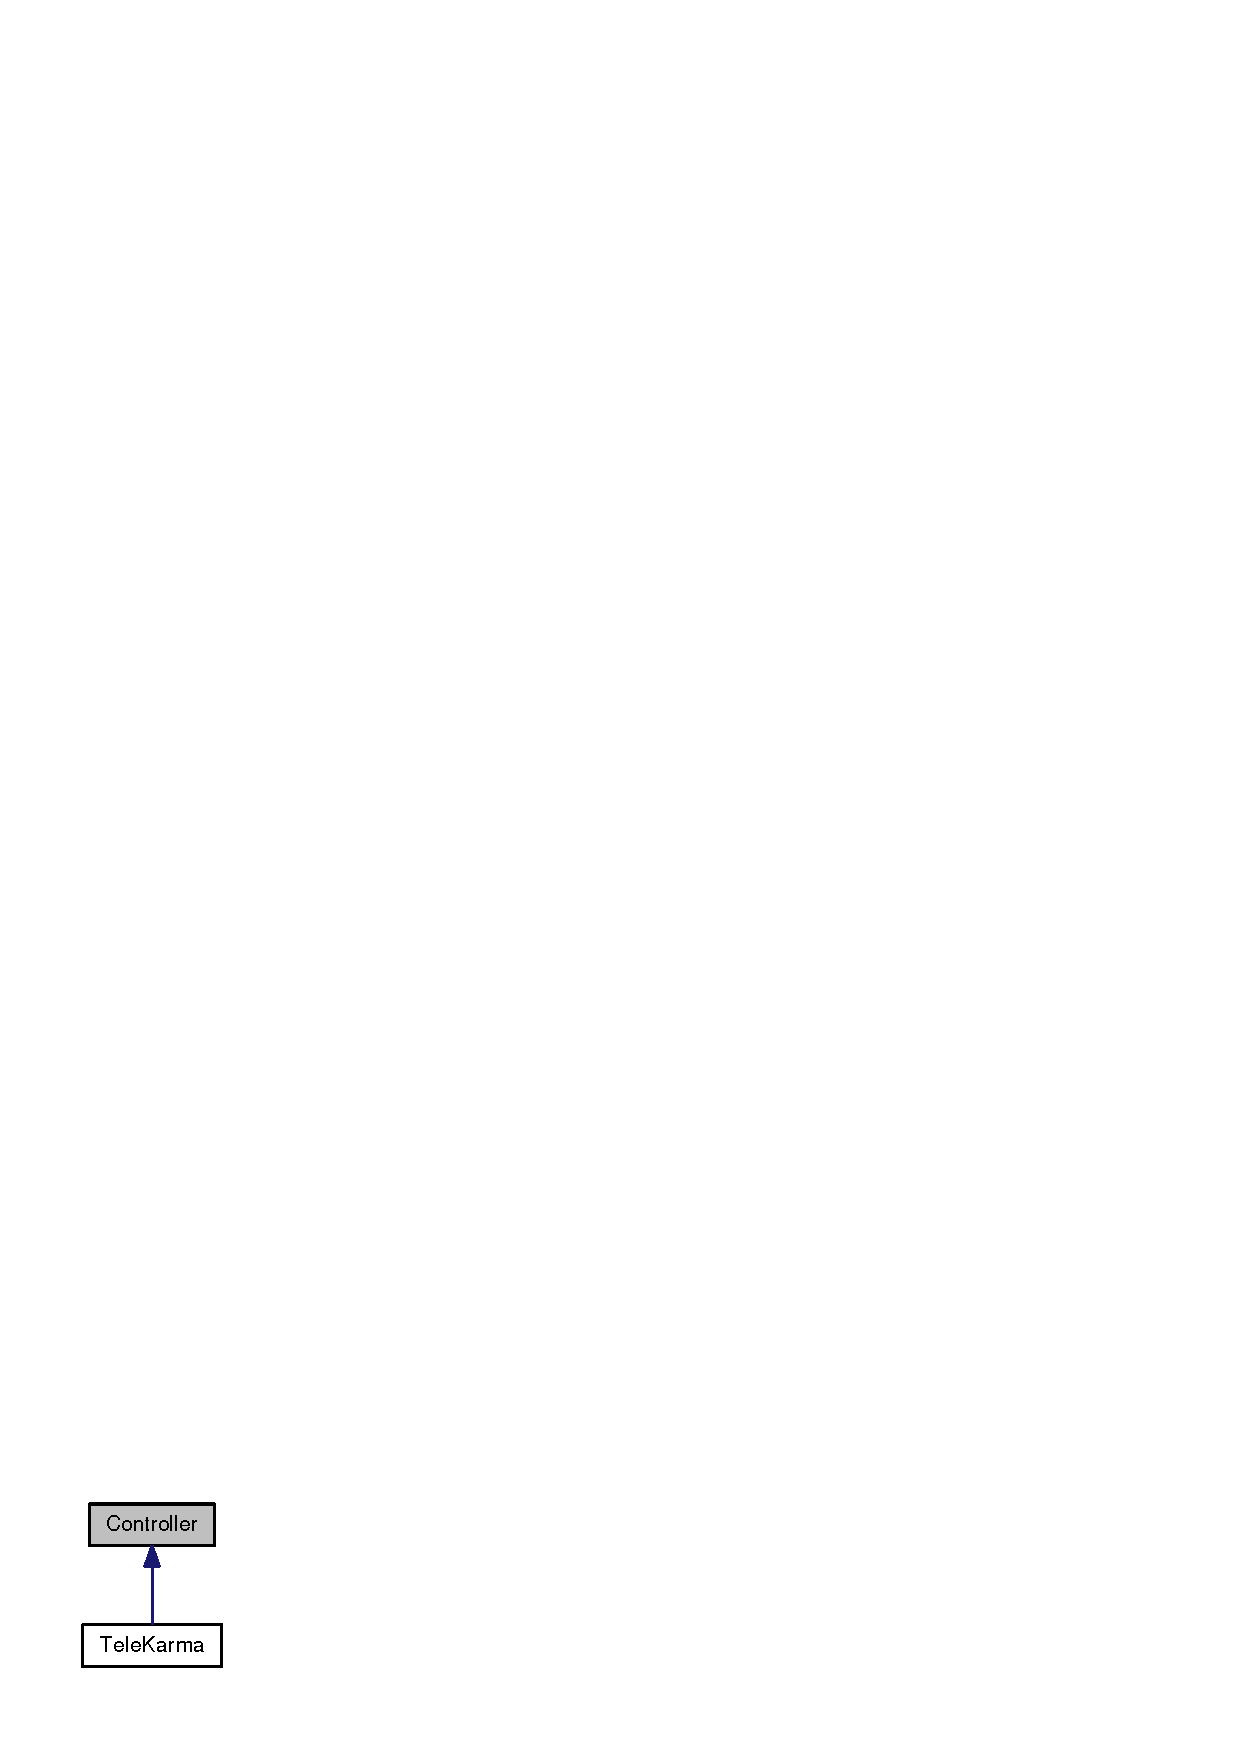
\includegraphics[width=110pt]{classController__inherit__graph}
\end{center}
\end{figure}
Collaboration diagram for Controller:\nopagebreak
\begin{figure}[H]
\begin{center}
\leavevmode

\includegraphics[width=245pt]{classController__coll__graph}
\end{center}
\end{figure}
\subsection*{Public Member Functions}
\begin{CompactItemize}
\item 
\hyperlink{classController_a3ca66cfc1e32af3f9b7563acf494277}{Controller} (\hyperlink{classModel}{Model} $\ast$\hyperlink{classController_6f6ea54052742d3940adfcfce885bae9}{model})
\item 
virtual void \hyperlink{classController_efeb521047c5b5d1c3f97290d015cacf}{Main} ()=0
\end{CompactItemize}
\subsection*{Protected Attributes}
\begin{CompactItemize}
\item 
\hyperlink{classModel}{Model} $\ast$ \hyperlink{classController_6f6ea54052742d3940adfcfce885bae9}{model}
\end{CompactItemize}


\subsection{Constructor \& Destructor Documentation}
\hypertarget{classController_a3ca66cfc1e32af3f9b7563acf494277}{
\index{Controller@{Controller}!Controller@{Controller}}
\index{Controller@{Controller}!Controller@{Controller}}
\subsubsection[{Controller}]{\setlength{\rightskip}{0pt plus 5cm}Controller::Controller ({\bf Model} $\ast$ {\em model})}}
\label{classController_a3ca66cfc1e32af3f9b7563acf494277}




\subsection{Member Function Documentation}
\hypertarget{classController_efeb521047c5b5d1c3f97290d015cacf}{
\index{Controller@{Controller}!Main@{Main}}
\index{Main@{Main}!Controller@{Controller}}
\subsubsection[{Main}]{\setlength{\rightskip}{0pt plus 5cm}virtual void Controller::Main ()\hspace{0.3cm}{\tt  \mbox{[}pure virtual\mbox{]}}}}
\label{classController_efeb521047c5b5d1c3f97290d015cacf}




Implemented in \hyperlink{classTeleKarma_addd554bf6335422cc896c894005a031}{TeleKarma}.

\subsection{Member Data Documentation}
\hypertarget{classController_6f6ea54052742d3940adfcfce885bae9}{
\index{Controller@{Controller}!model@{model}}
\index{model@{model}!Controller@{Controller}}
\subsubsection[{model}]{\setlength{\rightskip}{0pt plus 5cm}{\bf Model}$\ast$ {\bf Controller::model}\hspace{0.3cm}{\tt  \mbox{[}protected\mbox{]}}}}
\label{classController_6f6ea54052742d3940adfcfce885bae9}




The documentation for this class was generated from the following files:\begin{CompactItemize}
\item 
\hyperlink{controller_8h}{controller.h}\item 
\hyperlink{controller_8cpp}{controller.cpp}\end{CompactItemize}

\hypertarget{classDialAction}{
\section{DialAction Class Reference}
\label{classDialAction}\index{DialAction@{DialAction}}
}
{\tt \#include $<$action.h$>$}

Inheritance diagram for DialAction:\nopagebreak
\begin{figure}[H]
\begin{center}
\leavevmode
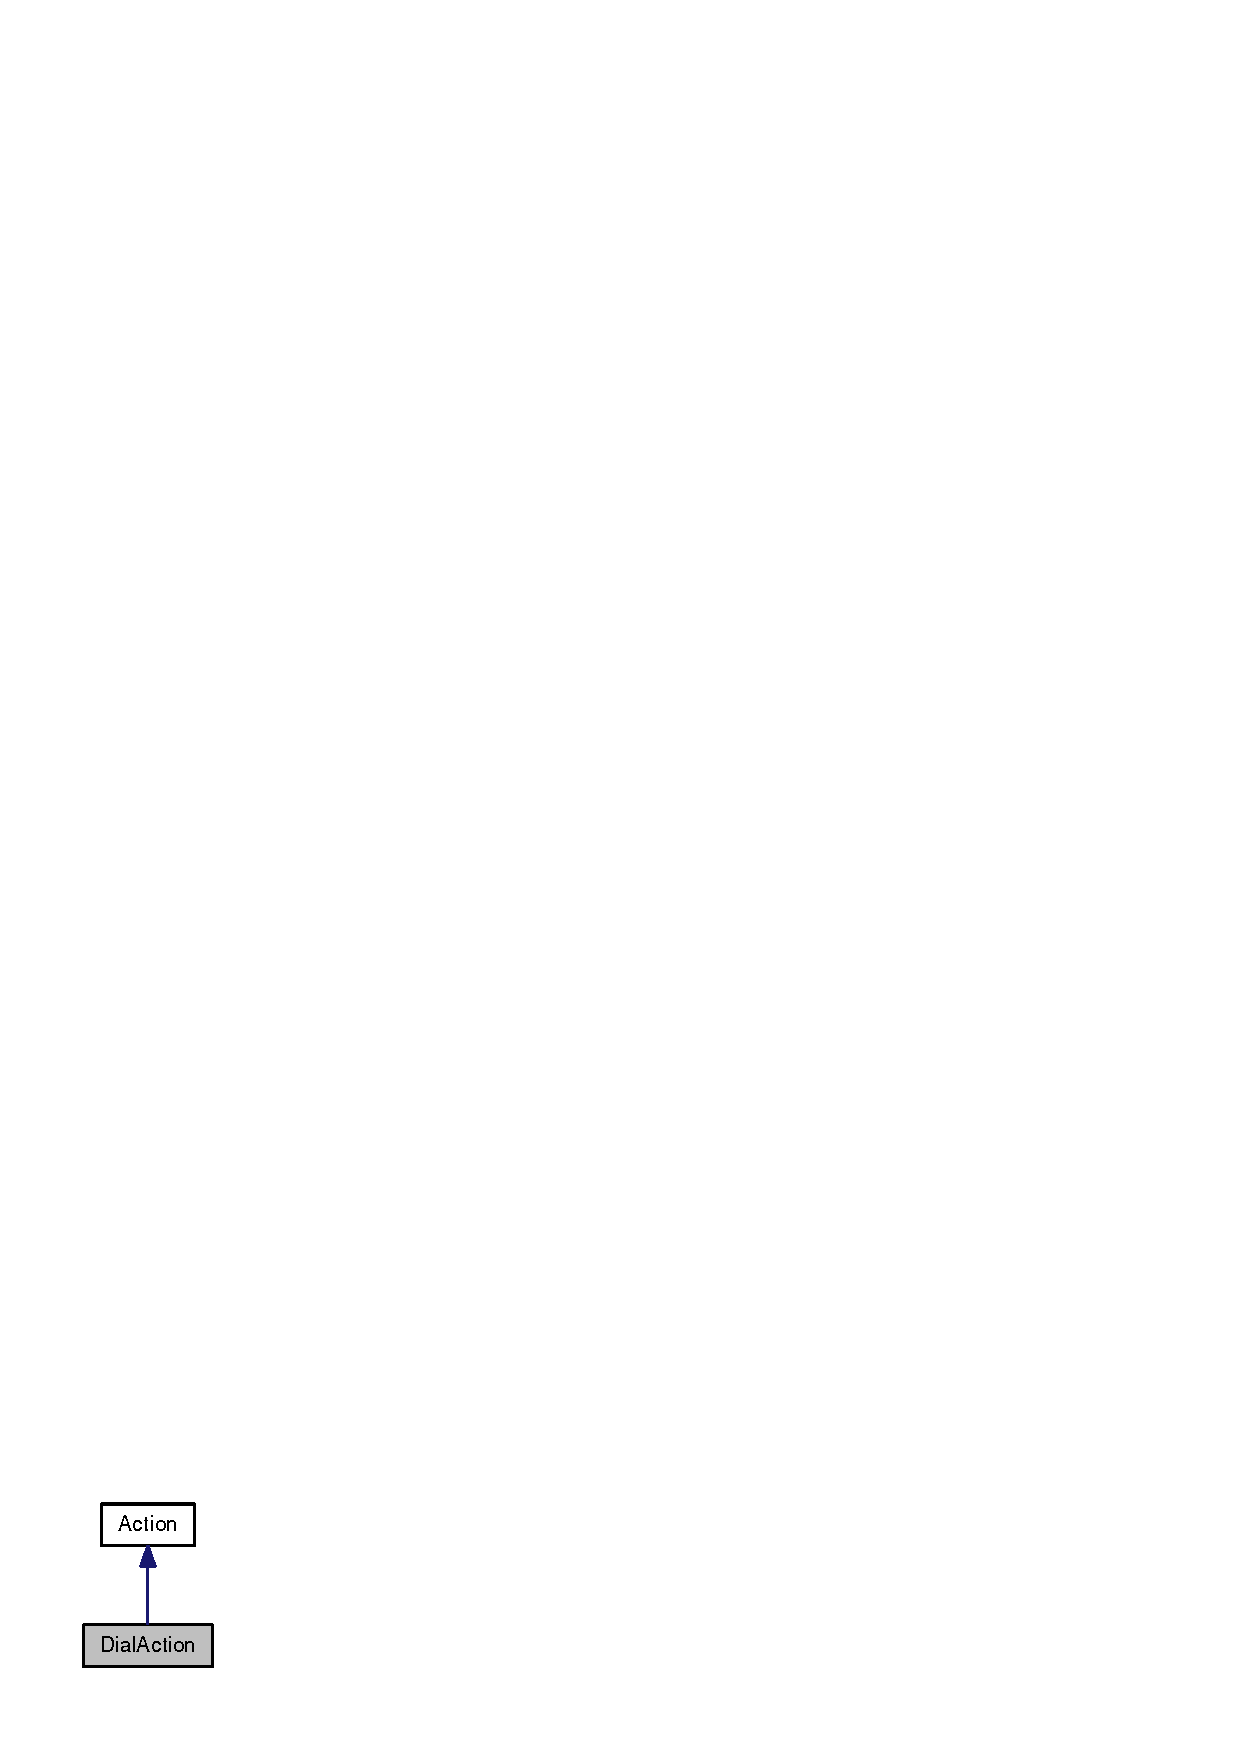
\includegraphics[width=106pt]{classDialAction__inherit__graph}
\end{center}
\end{figure}
Collaboration diagram for DialAction:\nopagebreak
\begin{figure}[H]
\begin{center}
\leavevmode

\includegraphics[width=106pt]{classDialAction__coll__graph}
\end{center}
\end{figure}
\subsection*{Public Member Functions}
\begin{CompactItemize}
\item 
\hyperlink{classDialAction_a6a4f34c622b886eedb04dca71e6baf7}{DialAction} (const PString \&\hyperlink{classDialAction_bd0ac2dd8e233138e05392eee0c743c7}{dest}, int \hyperlink{classAction_51e5d56a6aa4a037e90df19587a225c7}{turn})
\end{CompactItemize}
\subsection*{Public Attributes}
\begin{CompactItemize}
\item 
const PString \hyperlink{classDialAction_bd0ac2dd8e233138e05392eee0c743c7}{dest}
\end{CompactItemize}


\subsection{Constructor \& Destructor Documentation}
\hypertarget{classDialAction_a6a4f34c622b886eedb04dca71e6baf7}{
\index{DialAction@{DialAction}!DialAction@{DialAction}}
\index{DialAction@{DialAction}!DialAction@{DialAction}}
\subsubsection[{DialAction}]{\setlength{\rightskip}{0pt plus 5cm}DialAction::DialAction (const PString \& {\em dest}, \/  int {\em turn})\hspace{0.3cm}{\tt  \mbox{[}inline\mbox{]}}}}
\label{classDialAction_a6a4f34c622b886eedb04dca71e6baf7}




\subsection{Member Data Documentation}
\hypertarget{classDialAction_bd0ac2dd8e233138e05392eee0c743c7}{
\index{DialAction@{DialAction}!dest@{dest}}
\index{dest@{dest}!DialAction@{DialAction}}
\subsubsection[{dest}]{\setlength{\rightskip}{0pt plus 5cm}const PString {\bf DialAction::dest}}}
\label{classDialAction_bd0ac2dd8e233138e05392eee0c743c7}




The documentation for this class was generated from the following file:\begin{CompactItemize}
\item 
\hyperlink{action_8h}{action.h}\end{CompactItemize}

\hypertarget{classDialPad}{
\section{DialPad Class Reference}
\label{classDialPad}\index{DialPad@{DialPad}}
}
Dial pad for touch tone transmission.  


{\tt \#include $<$gui.h$>$}

Collaboration diagram for DialPad:\nopagebreak
\begin{figure}[H]
\begin{center}
\leavevmode
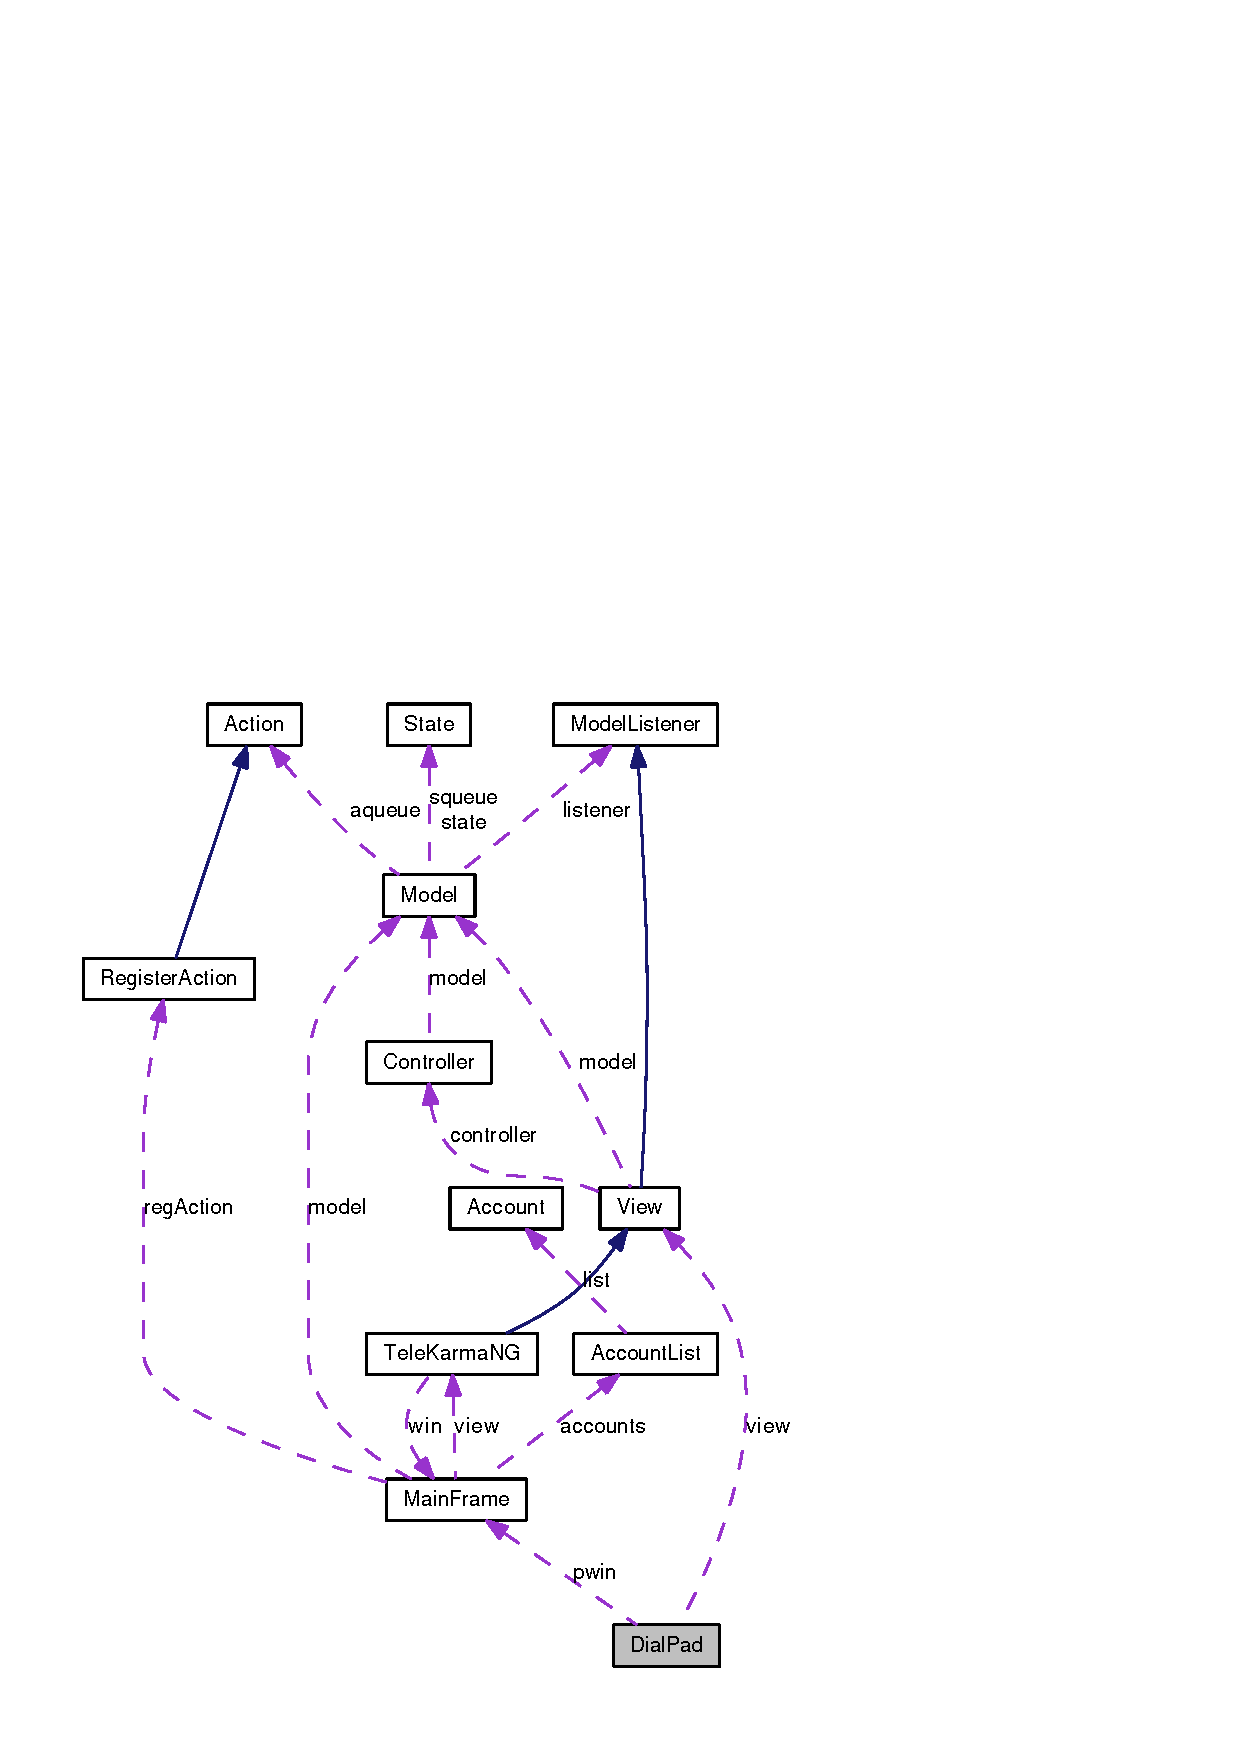
\includegraphics[height=400pt]{classDialPad__coll__graph}
\end{center}
\end{figure}
\subsection*{Public Member Functions}
\begin{CompactItemize}
\item 
\hyperlink{classDialPad_4f25385be59567e595bad984693ec01f}{DialPad} (\hyperlink{classMainFrame}{MainFrame} $\ast$pwin, \hyperlink{classView}{View} $\ast$view)
\begin{CompactList}\small\item\em Constructor. \item\end{CompactList}\item 
void \hyperlink{classDialPad_d3bc3a3c043049ef4d396768dfade82f}{OnClose} (wxCloseEvent \&event)
\begin{CompactList}\small\item\em Responds to system close events. \item\end{CompactList}\item 
void \hyperlink{classDialPad_5b55819a3a90ff5abf9e1c6f7c36126c}{OnPressOne} (wxCommandEvent \&event)
\begin{CompactList}\small\item\em Sends a touch tone action to model upon click of associated button. \item\end{CompactList}\item 
void \hyperlink{classDialPad_dbf2a305725f08af6237df2c50eb92b6}{OnPressTwo} (wxCommandEvent \&event)
\begin{CompactList}\small\item\em Sends a touch tone action to model upon click of associated button. \item\end{CompactList}\item 
void \hyperlink{classDialPad_32214f7d206c448a7f25ceabaa32bdcb}{OnPressThree} (wxCommandEvent \&event)
\begin{CompactList}\small\item\em Sends a touch tone action to model upon click of associated button. \item\end{CompactList}\item 
void \hyperlink{classDialPad_3ba175a7000657d2a79ccbb858b5803f}{OnPressFour} (wxCommandEvent \&event)
\begin{CompactList}\small\item\em Sends a touch tone action to model upon click of associated button. \item\end{CompactList}\item 
void \hyperlink{classDialPad_1117cbca8f1075f55097b8a2c3859d7f}{OnPressFive} (wxCommandEvent \&event)
\begin{CompactList}\small\item\em Sends a touch tone action to model upon click of associated button. \item\end{CompactList}\item 
void \hyperlink{classDialPad_d6212054f7d5ff5a167376265b377bc7}{OnPressSix} (wxCommandEvent \&event)
\begin{CompactList}\small\item\em Sends a touch tone action to model upon click of associated button. \item\end{CompactList}\item 
void \hyperlink{classDialPad_fdfbc9b26eabdd85d512a21aaf9bf883}{OnPressSeven} (wxCommandEvent \&event)
\begin{CompactList}\small\item\em Sends a touch tone action to model upon click of associated button. \item\end{CompactList}\item 
void \hyperlink{classDialPad_a12bc9af8ce8a3fdad15fa55f70ea5c0}{OnPressEight} (wxCommandEvent \&event)
\begin{CompactList}\small\item\em Sends a touch tone action to model upon click of associated button. \item\end{CompactList}\item 
void \hyperlink{classDialPad_fd908470bb6b43597ba2169bfd6e0271}{OnPressNine} (wxCommandEvent \&event)
\begin{CompactList}\small\item\em Sends a touch tone action to model upon click of associated button. \item\end{CompactList}\item 
void \hyperlink{classDialPad_69cd65cf785135fdfa246882965b77ec}{OnPressStar} (wxCommandEvent \&event)
\begin{CompactList}\small\item\em Sends a touch tone action to model upon click of associated button. \item\end{CompactList}\item 
void \hyperlink{classDialPad_4e71463b25b3004ea30cfc64c298a03c}{OnPressZero} (wxCommandEvent \&event)
\begin{CompactList}\small\item\em Sends a touch tone action to model upon click of associated button. \item\end{CompactList}\item 
void \hyperlink{classDialPad_19c18972706083103c18228c64a0acbb}{OnPressPound} (wxCommandEvent \&event)
\begin{CompactList}\small\item\em Sends a touch tone action to model upon click of associated button. \item\end{CompactList}\end{CompactItemize}


\subsection{Detailed Description}
Dial pad for touch tone transmission. 

Sends fixed-duration touch tones when buttons are released, rather sending a touch tone continuously while the button is depressed. 

\subsection{Constructor \& Destructor Documentation}
\hypertarget{classDialPad_4f25385be59567e595bad984693ec01f}{
\index{DialPad@{DialPad}!DialPad@{DialPad}}
\index{DialPad@{DialPad}!DialPad@{DialPad}}
\subsubsection[{DialPad}]{\setlength{\rightskip}{0pt plus 5cm}DialPad::DialPad ({\bf MainFrame} $\ast$ {\em pwin}, \/  {\bf View} $\ast$ {\em view})}}
\label{classDialPad_4f25385be59567e595bad984693ec01f}


Constructor. 

\begin{Desc}
\item[Parameters:]
\begin{description}
\item[{\em pwin}]parent window. \item[{\em view}]for access to \hyperlink{classView_cb2535000de204a5e4202c6ecce64666}{View\#DoAction(Action $\ast$)}. \end{description}
\end{Desc}


\subsection{Member Function Documentation}
\hypertarget{classDialPad_d3bc3a3c043049ef4d396768dfade82f}{
\index{DialPad@{DialPad}!OnClose@{OnClose}}
\index{OnClose@{OnClose}!DialPad@{DialPad}}
\subsubsection[{OnClose}]{\setlength{\rightskip}{0pt plus 5cm}void DialPad::OnClose (wxCloseEvent \& {\em event})}}
\label{classDialPad_d3bc3a3c043049ef4d396768dfade82f}


Responds to system close events. 

Notifies pwin. Exclusively for use by wxWidgets event dispatcher. \hypertarget{classDialPad_a12bc9af8ce8a3fdad15fa55f70ea5c0}{
\index{DialPad@{DialPad}!OnPressEight@{OnPressEight}}
\index{OnPressEight@{OnPressEight}!DialPad@{DialPad}}
\subsubsection[{OnPressEight}]{\setlength{\rightskip}{0pt plus 5cm}void DialPad::OnPressEight (wxCommandEvent \& {\em event})}}
\label{classDialPad_a12bc9af8ce8a3fdad15fa55f70ea5c0}


Sends a touch tone action to model upon click of associated button. 

Exclusively for use by wxWidgets event dispatcher. \hypertarget{classDialPad_1117cbca8f1075f55097b8a2c3859d7f}{
\index{DialPad@{DialPad}!OnPressFive@{OnPressFive}}
\index{OnPressFive@{OnPressFive}!DialPad@{DialPad}}
\subsubsection[{OnPressFive}]{\setlength{\rightskip}{0pt plus 5cm}void DialPad::OnPressFive (wxCommandEvent \& {\em event})}}
\label{classDialPad_1117cbca8f1075f55097b8a2c3859d7f}


Sends a touch tone action to model upon click of associated button. 

Exclusively for use by wxWidgets event dispatcher. \hypertarget{classDialPad_3ba175a7000657d2a79ccbb858b5803f}{
\index{DialPad@{DialPad}!OnPressFour@{OnPressFour}}
\index{OnPressFour@{OnPressFour}!DialPad@{DialPad}}
\subsubsection[{OnPressFour}]{\setlength{\rightskip}{0pt plus 5cm}void DialPad::OnPressFour (wxCommandEvent \& {\em event})}}
\label{classDialPad_3ba175a7000657d2a79ccbb858b5803f}


Sends a touch tone action to model upon click of associated button. 

Exclusively for use by wxWidgets event dispatcher. \hypertarget{classDialPad_fd908470bb6b43597ba2169bfd6e0271}{
\index{DialPad@{DialPad}!OnPressNine@{OnPressNine}}
\index{OnPressNine@{OnPressNine}!DialPad@{DialPad}}
\subsubsection[{OnPressNine}]{\setlength{\rightskip}{0pt plus 5cm}void DialPad::OnPressNine (wxCommandEvent \& {\em event})}}
\label{classDialPad_fd908470bb6b43597ba2169bfd6e0271}


Sends a touch tone action to model upon click of associated button. 

Exclusively for use by wxWidgets event dispatcher. \hypertarget{classDialPad_5b55819a3a90ff5abf9e1c6f7c36126c}{
\index{DialPad@{DialPad}!OnPressOne@{OnPressOne}}
\index{OnPressOne@{OnPressOne}!DialPad@{DialPad}}
\subsubsection[{OnPressOne}]{\setlength{\rightskip}{0pt plus 5cm}void DialPad::OnPressOne (wxCommandEvent \& {\em event})}}
\label{classDialPad_5b55819a3a90ff5abf9e1c6f7c36126c}


Sends a touch tone action to model upon click of associated button. 

Exclusively for use by wxWidgets event dispatcher. \hypertarget{classDialPad_19c18972706083103c18228c64a0acbb}{
\index{DialPad@{DialPad}!OnPressPound@{OnPressPound}}
\index{OnPressPound@{OnPressPound}!DialPad@{DialPad}}
\subsubsection[{OnPressPound}]{\setlength{\rightskip}{0pt plus 5cm}void DialPad::OnPressPound (wxCommandEvent \& {\em event})}}
\label{classDialPad_19c18972706083103c18228c64a0acbb}


Sends a touch tone action to model upon click of associated button. 

Exclusively for use by wxWidgets event dispatcher. \hypertarget{classDialPad_fdfbc9b26eabdd85d512a21aaf9bf883}{
\index{DialPad@{DialPad}!OnPressSeven@{OnPressSeven}}
\index{OnPressSeven@{OnPressSeven}!DialPad@{DialPad}}
\subsubsection[{OnPressSeven}]{\setlength{\rightskip}{0pt plus 5cm}void DialPad::OnPressSeven (wxCommandEvent \& {\em event})}}
\label{classDialPad_fdfbc9b26eabdd85d512a21aaf9bf883}


Sends a touch tone action to model upon click of associated button. 

Exclusively for use by wxWidgets event dispatcher. \hypertarget{classDialPad_d6212054f7d5ff5a167376265b377bc7}{
\index{DialPad@{DialPad}!OnPressSix@{OnPressSix}}
\index{OnPressSix@{OnPressSix}!DialPad@{DialPad}}
\subsubsection[{OnPressSix}]{\setlength{\rightskip}{0pt plus 5cm}void DialPad::OnPressSix (wxCommandEvent \& {\em event})}}
\label{classDialPad_d6212054f7d5ff5a167376265b377bc7}


Sends a touch tone action to model upon click of associated button. 

Exclusively for use by wxWidgets event dispatcher. Sends a touch tone action to model upon click of associated button. Exclusively for use by wxWidgets event dispatcher. \hypertarget{classDialPad_69cd65cf785135fdfa246882965b77ec}{
\index{DialPad@{DialPad}!OnPressStar@{OnPressStar}}
\index{OnPressStar@{OnPressStar}!DialPad@{DialPad}}
\subsubsection[{OnPressStar}]{\setlength{\rightskip}{0pt plus 5cm}void DialPad::OnPressStar (wxCommandEvent \& {\em event})}}
\label{classDialPad_69cd65cf785135fdfa246882965b77ec}


Sends a touch tone action to model upon click of associated button. 

Exclusively for use by wxWidgets event dispatcher. \hypertarget{classDialPad_32214f7d206c448a7f25ceabaa32bdcb}{
\index{DialPad@{DialPad}!OnPressThree@{OnPressThree}}
\index{OnPressThree@{OnPressThree}!DialPad@{DialPad}}
\subsubsection[{OnPressThree}]{\setlength{\rightskip}{0pt plus 5cm}void DialPad::OnPressThree (wxCommandEvent \& {\em event})}}
\label{classDialPad_32214f7d206c448a7f25ceabaa32bdcb}


Sends a touch tone action to model upon click of associated button. 

Exclusively for use by wxWidgets event dispatcher. \hypertarget{classDialPad_dbf2a305725f08af6237df2c50eb92b6}{
\index{DialPad@{DialPad}!OnPressTwo@{OnPressTwo}}
\index{OnPressTwo@{OnPressTwo}!DialPad@{DialPad}}
\subsubsection[{OnPressTwo}]{\setlength{\rightskip}{0pt plus 5cm}void DialPad::OnPressTwo (wxCommandEvent \& {\em event})}}
\label{classDialPad_dbf2a305725f08af6237df2c50eb92b6}


Sends a touch tone action to model upon click of associated button. 

Exclusively for use by wxWidgets event dispatcher. \hypertarget{classDialPad_4e71463b25b3004ea30cfc64c298a03c}{
\index{DialPad@{DialPad}!OnPressZero@{OnPressZero}}
\index{OnPressZero@{OnPressZero}!DialPad@{DialPad}}
\subsubsection[{OnPressZero}]{\setlength{\rightskip}{0pt plus 5cm}void DialPad::OnPressZero (wxCommandEvent \& {\em event})}}
\label{classDialPad_4e71463b25b3004ea30cfc64c298a03c}


Sends a touch tone action to model upon click of associated button. 

Exclusively for use by wxWidgets event dispatcher. 

The documentation for this class was generated from the following files:\begin{CompactItemize}
\item 
\hyperlink{gui_8h}{gui.h}\item 
\hyperlink{gui_8cpp}{gui.cpp}\end{CompactItemize}

\hypertarget{classDisconnectAction}{
\section{DisconnectAction Class Reference}
\label{classDisconnectAction}\index{DisconnectAction@{DisconnectAction}}
}
{\tt \#include $<$action.h$>$}

Inheritance diagram for DisconnectAction:\nopagebreak
\begin{figure}[H]
\begin{center}
\leavevmode
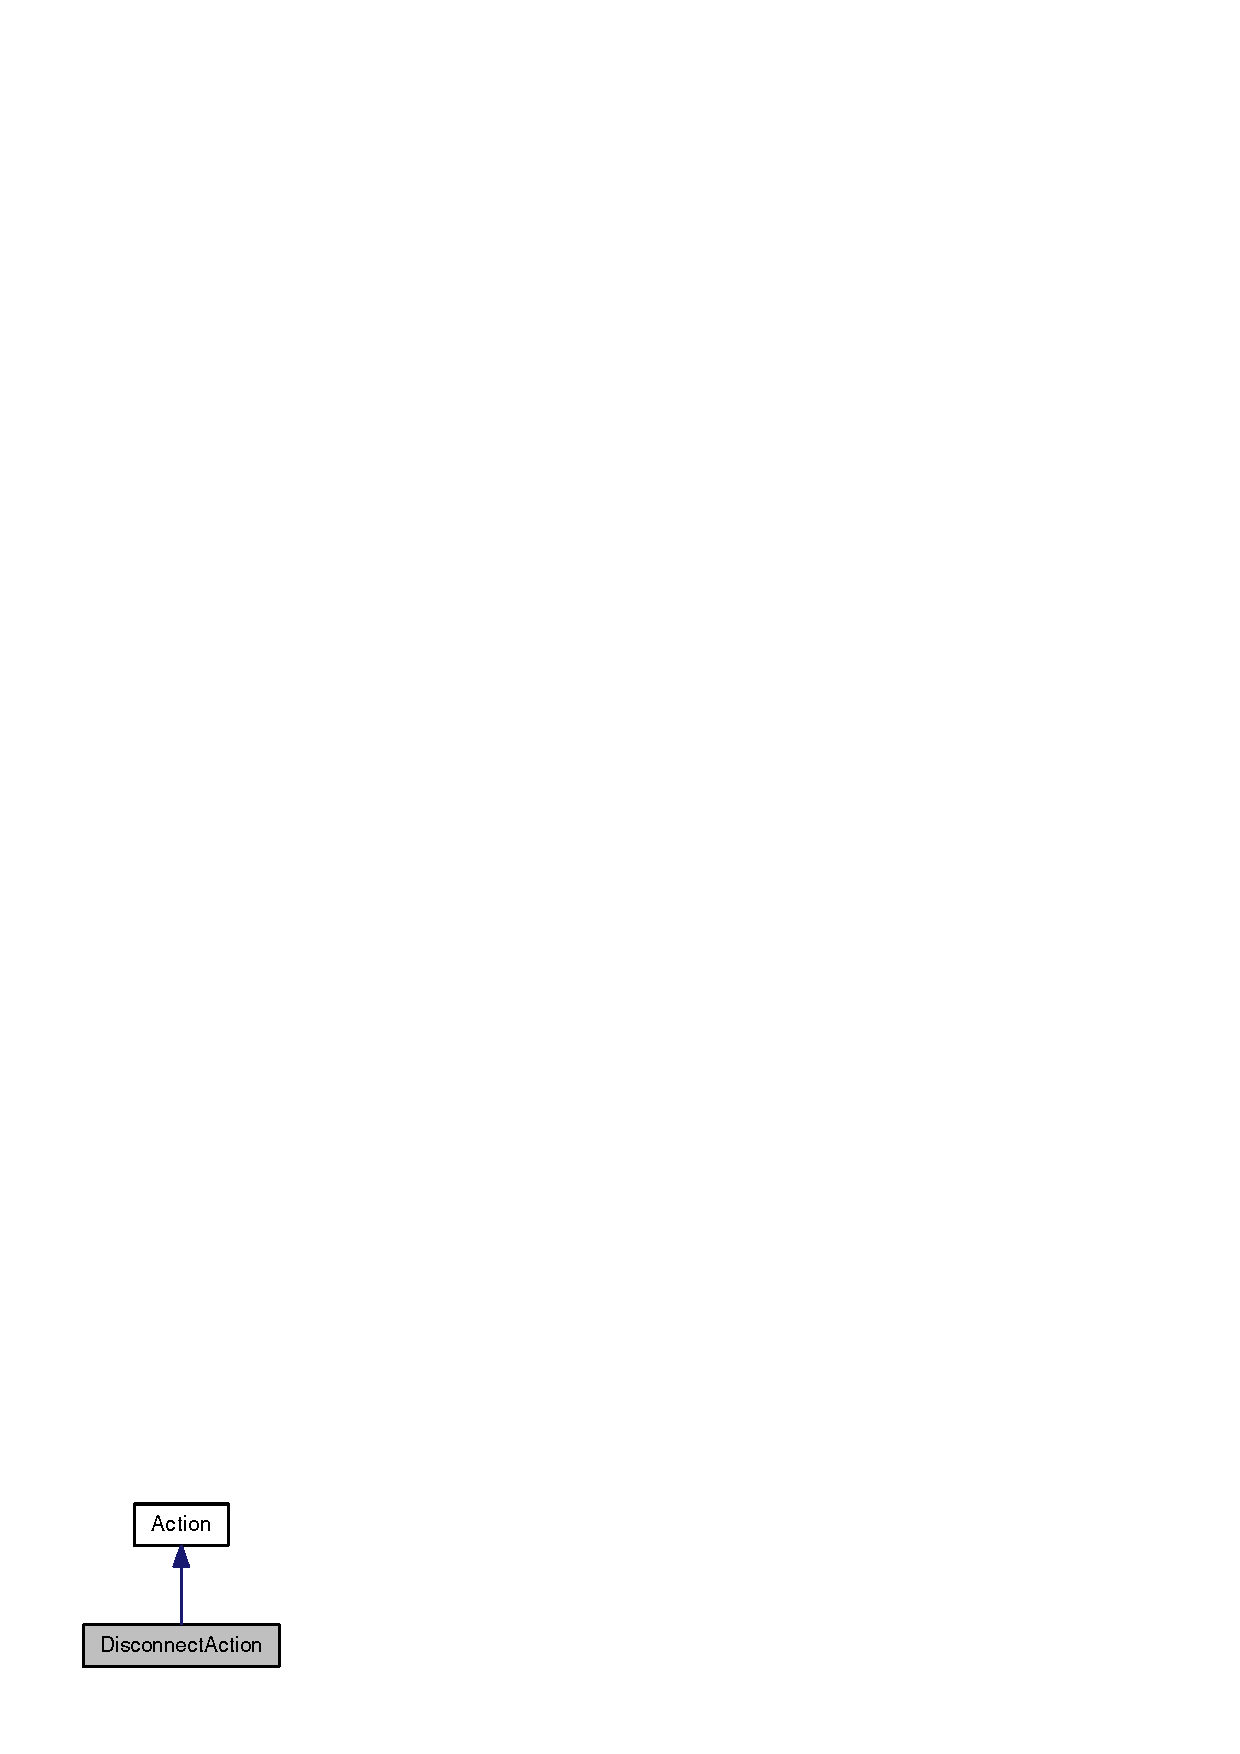
\includegraphics[width=138pt]{classDisconnectAction__inherit__graph}
\end{center}
\end{figure}
Collaboration diagram for DisconnectAction:\nopagebreak
\begin{figure}[H]
\begin{center}
\leavevmode
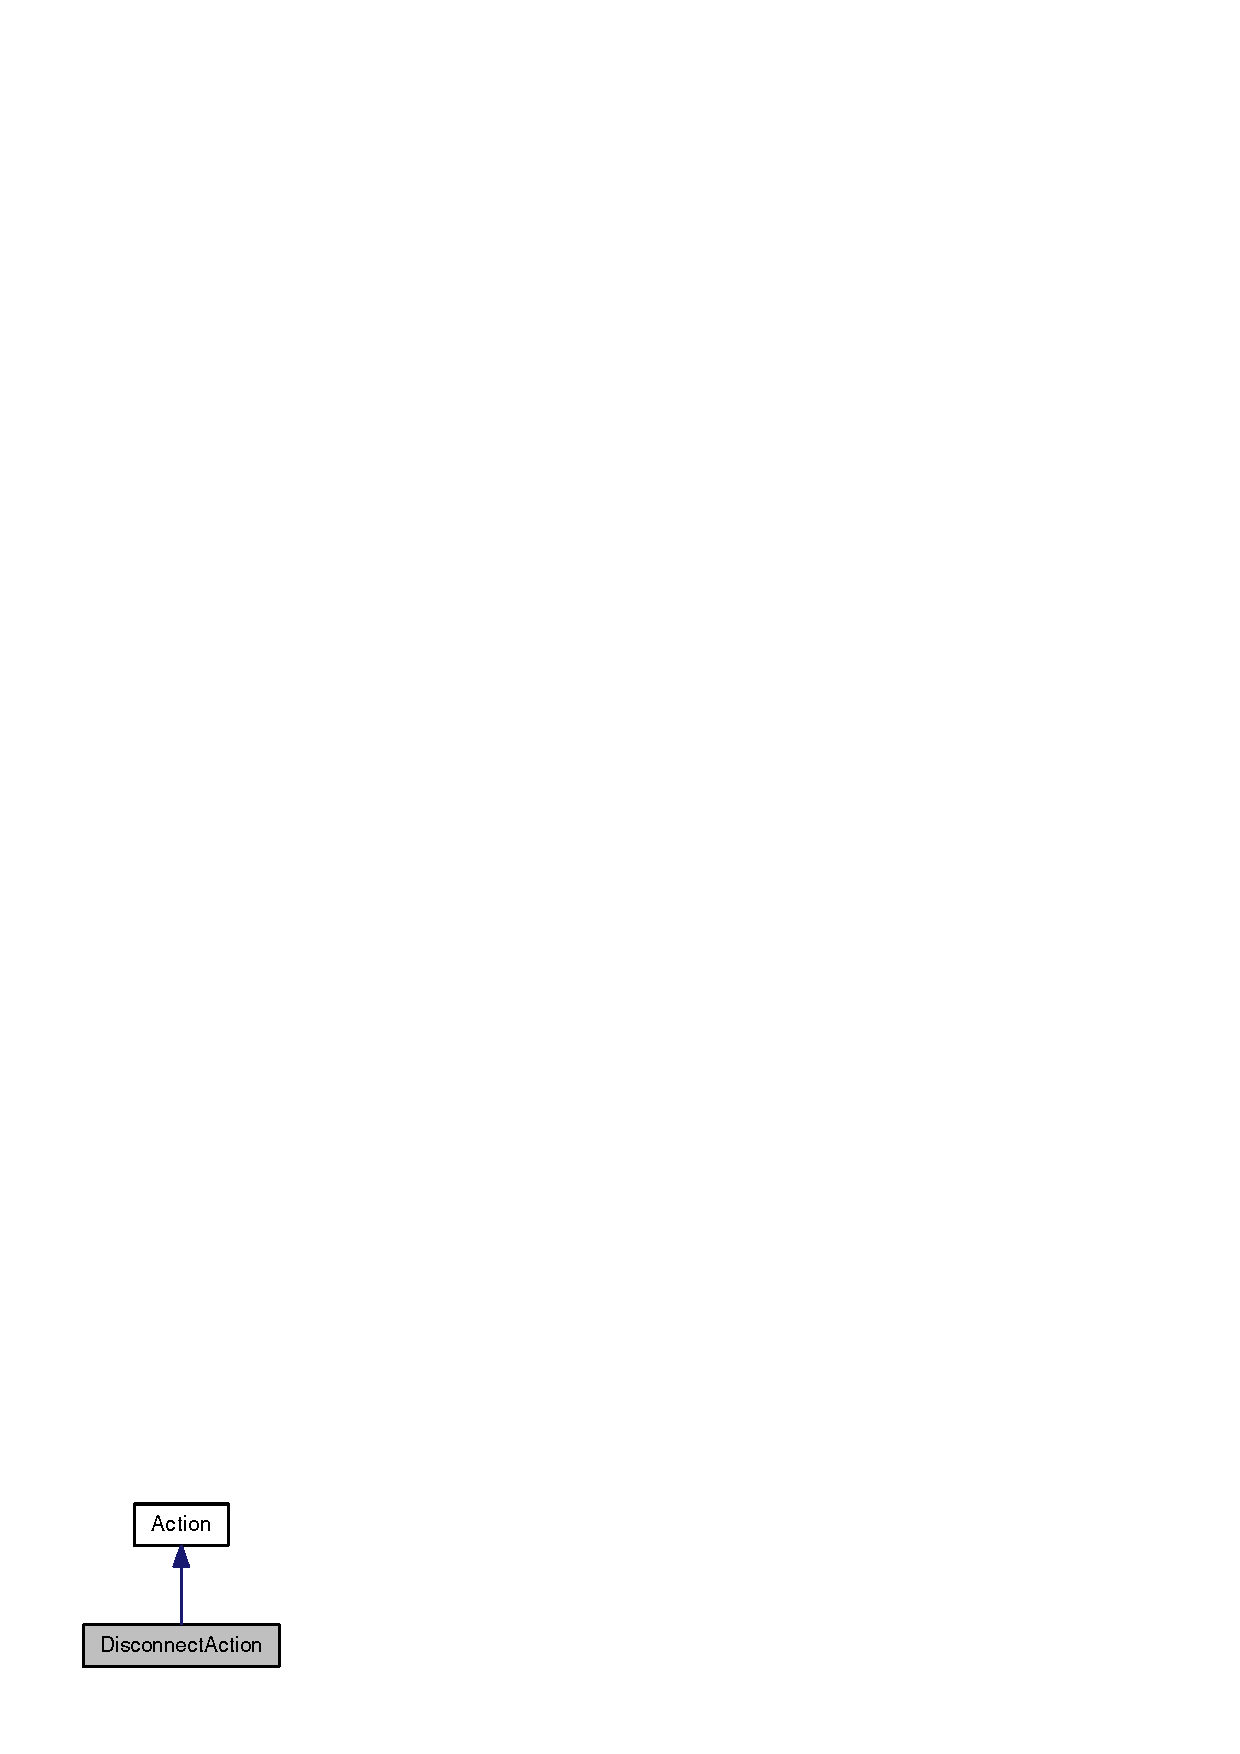
\includegraphics[width=138pt]{classDisconnectAction__coll__graph}
\end{center}
\end{figure}
\subsection*{Public Member Functions}
\begin{CompactItemize}
\item 
\hyperlink{classDisconnectAction_7b9d0cdf0f6baac981a67952aa595014}{DisconnectAction} (int \hyperlink{classAction_51e5d56a6aa4a037e90df19587a225c7}{turn})
\end{CompactItemize}


\subsection{Constructor \& Destructor Documentation}
\hypertarget{classDisconnectAction_7b9d0cdf0f6baac981a67952aa595014}{
\index{DisconnectAction@{DisconnectAction}!DisconnectAction@{DisconnectAction}}
\index{DisconnectAction@{DisconnectAction}!DisconnectAction@{DisconnectAction}}
\subsubsection[{DisconnectAction}]{\setlength{\rightskip}{0pt plus 5cm}DisconnectAction::DisconnectAction (int {\em turn})\hspace{0.3cm}{\tt  \mbox{[}inline\mbox{]}}}}
\label{classDisconnectAction_7b9d0cdf0f6baac981a67952aa595014}




The documentation for this class was generated from the following file:\begin{CompactItemize}
\item 
\hyperlink{action_8h}{action.h}\end{CompactItemize}

\hypertarget{classHoldAction}{
\section{HoldAction Class Reference}
\label{classHoldAction}\index{HoldAction@{HoldAction}}
}
{\tt \#include $<$action.h$>$}

Inheritance diagram for HoldAction:\nopagebreak
\begin{figure}[H]
\begin{center}
\leavevmode
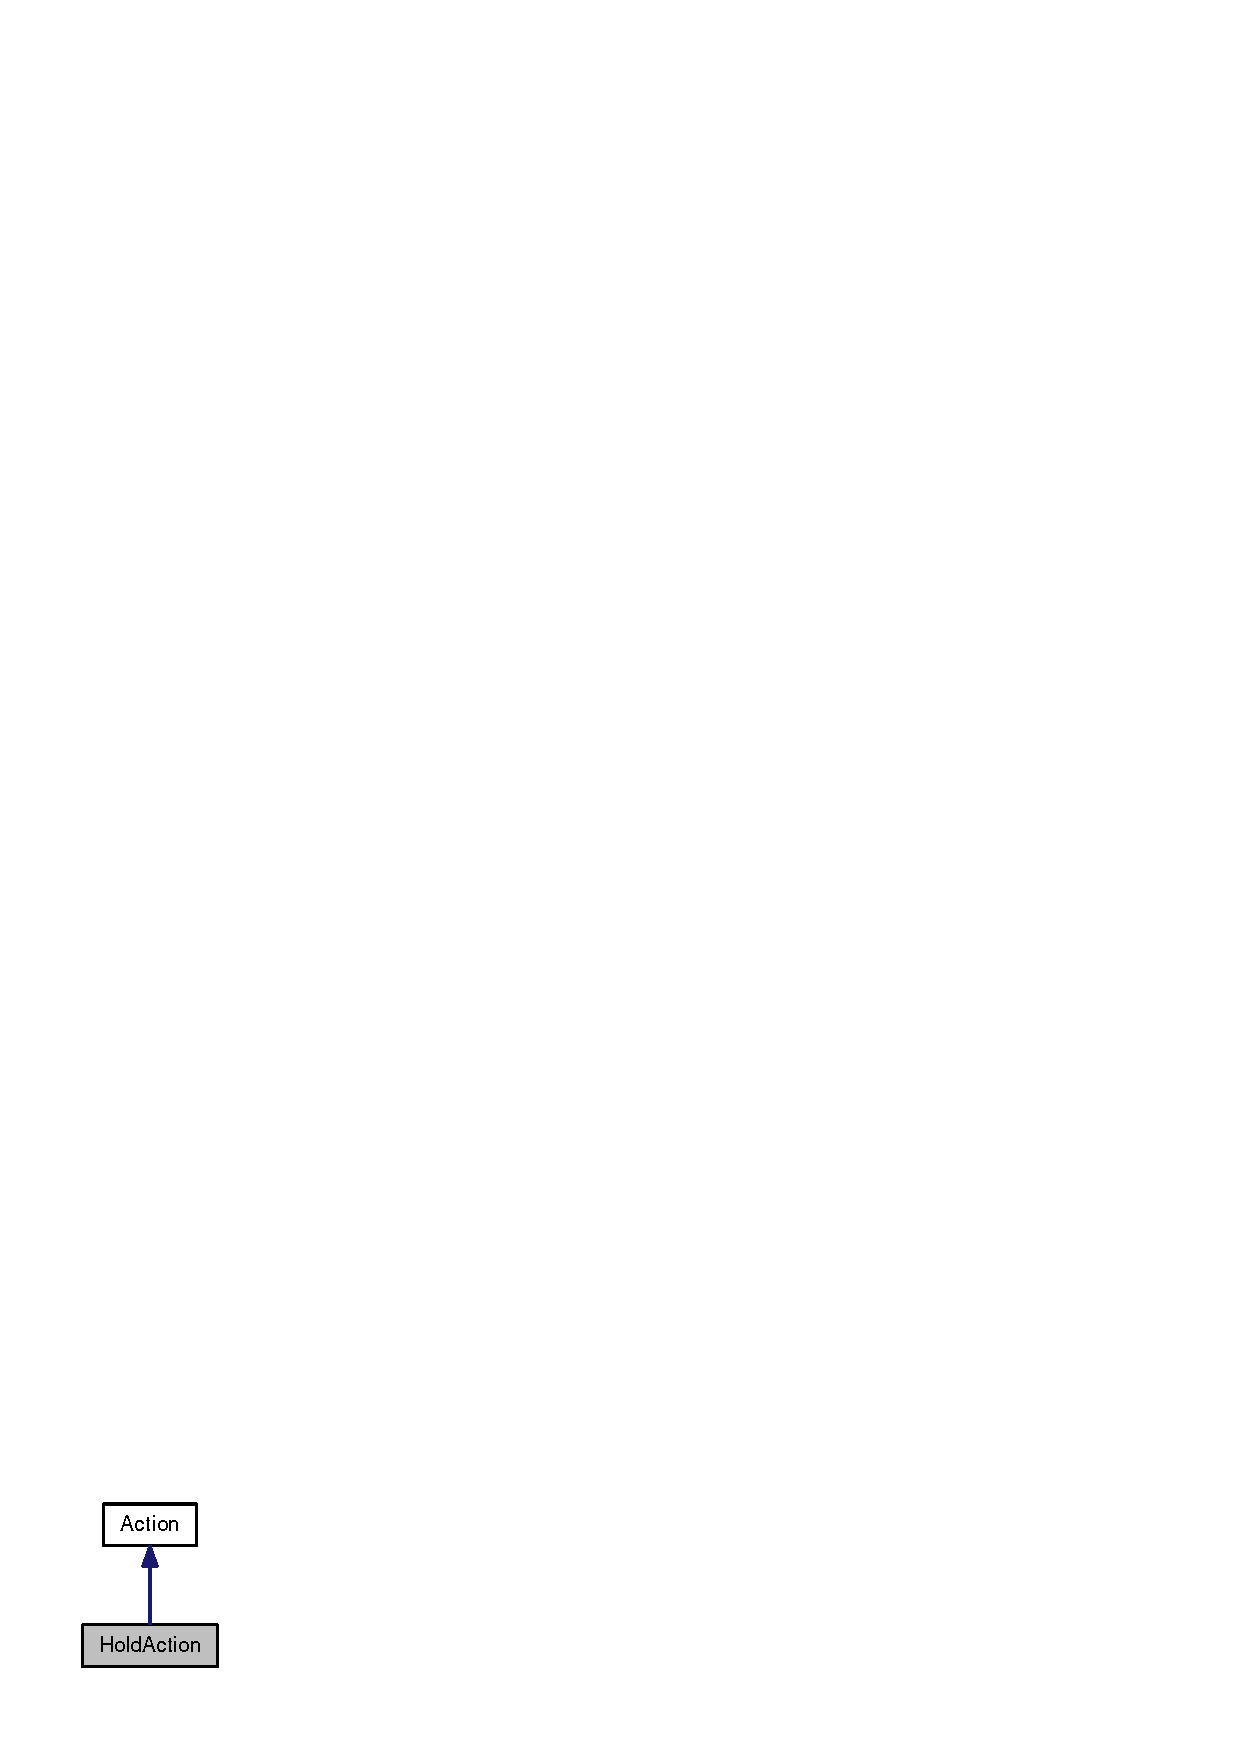
\includegraphics[width=108pt]{classHoldAction__inherit__graph}
\end{center}
\end{figure}
Collaboration diagram for HoldAction:\nopagebreak
\begin{figure}[H]
\begin{center}
\leavevmode

\includegraphics[width=108pt]{classHoldAction__coll__graph}
\end{center}
\end{figure}
\subsection*{Public Member Functions}
\begin{CompactItemize}
\item 
\hyperlink{classHoldAction_4af274044f62732dc5ffbb60d021e8ec}{HoldAction} (int \hyperlink{classAction_51e5d56a6aa4a037e90df19587a225c7}{turn})
\end{CompactItemize}


\subsection{Constructor \& Destructor Documentation}
\hypertarget{classHoldAction_4af274044f62732dc5ffbb60d021e8ec}{
\index{HoldAction@{HoldAction}!HoldAction@{HoldAction}}
\index{HoldAction@{HoldAction}!HoldAction@{HoldAction}}
\subsubsection[{HoldAction}]{\setlength{\rightskip}{0pt plus 5cm}HoldAction::HoldAction (int {\em turn})\hspace{0.3cm}{\tt  \mbox{[}inline\mbox{]}}}}
\label{classHoldAction_4af274044f62732dc5ffbb60d021e8ec}




The documentation for this class was generated from the following file:\begin{CompactItemize}
\item 
\hyperlink{action_8h}{action.h}\end{CompactItemize}

\hypertarget{classInitializeAction}{
\section{InitializeAction Class Reference}
\label{classInitializeAction}\index{InitializeAction@{InitializeAction}}
}
{\tt \#include $<$action.h$>$}

Inheritance diagram for InitializeAction:\nopagebreak
\begin{figure}[H]
\begin{center}
\leavevmode

\includegraphics[width=124pt]{classInitializeAction__inherit__graph}
\end{center}
\end{figure}
Collaboration diagram for InitializeAction:\nopagebreak
\begin{figure}[H]
\begin{center}
\leavevmode

\includegraphics[width=124pt]{classInitializeAction__coll__graph}
\end{center}
\end{figure}
\subsection*{Public Member Functions}
\begin{CompactItemize}
\item 
\hyperlink{classInitializeAction_984b7dd9f095a6601f81724bb7186587}{InitializeAction} (const PString \&\hyperlink{classInitializeAction_584d375d97a7b11ef7513dc709d9b8a5}{stunServer}, int \hyperlink{classAction_51e5d56a6aa4a037e90df19587a225c7}{turn})
\end{CompactItemize}
\subsection*{Public Attributes}
\begin{CompactItemize}
\item 
const PString \hyperlink{classInitializeAction_584d375d97a7b11ef7513dc709d9b8a5}{stunServer}
\end{CompactItemize}


\subsection{Constructor \& Destructor Documentation}
\hypertarget{classInitializeAction_984b7dd9f095a6601f81724bb7186587}{
\index{InitializeAction@{InitializeAction}!InitializeAction@{InitializeAction}}
\index{InitializeAction@{InitializeAction}!InitializeAction@{InitializeAction}}
\subsubsection[{InitializeAction}]{\setlength{\rightskip}{0pt plus 5cm}InitializeAction::InitializeAction (const PString \& {\em stunServer}, \/  int {\em turn})\hspace{0.3cm}{\tt  \mbox{[}inline\mbox{]}}}}
\label{classInitializeAction_984b7dd9f095a6601f81724bb7186587}




\subsection{Member Data Documentation}
\hypertarget{classInitializeAction_584d375d97a7b11ef7513dc709d9b8a5}{
\index{InitializeAction@{InitializeAction}!stunServer@{stunServer}}
\index{stunServer@{stunServer}!InitializeAction@{InitializeAction}}
\subsubsection[{stunServer}]{\setlength{\rightskip}{0pt plus 5cm}const PString {\bf InitializeAction::stunServer}}}
\label{classInitializeAction_584d375d97a7b11ef7513dc709d9b8a5}




The documentation for this class was generated from the following file:\begin{CompactItemize}
\item 
\hyperlink{action_8h}{action.h}\end{CompactItemize}

\hypertarget{classMainFrame}{
\section{MainFrame Class Reference}
\label{classMainFrame}\index{MainFrame@{MainFrame}}
}
The main window.  


{\tt \#include $<$gui.h$>$}

Collaboration diagram for MainFrame:\nopagebreak
\begin{figure}[H]
\begin{center}
\leavevmode
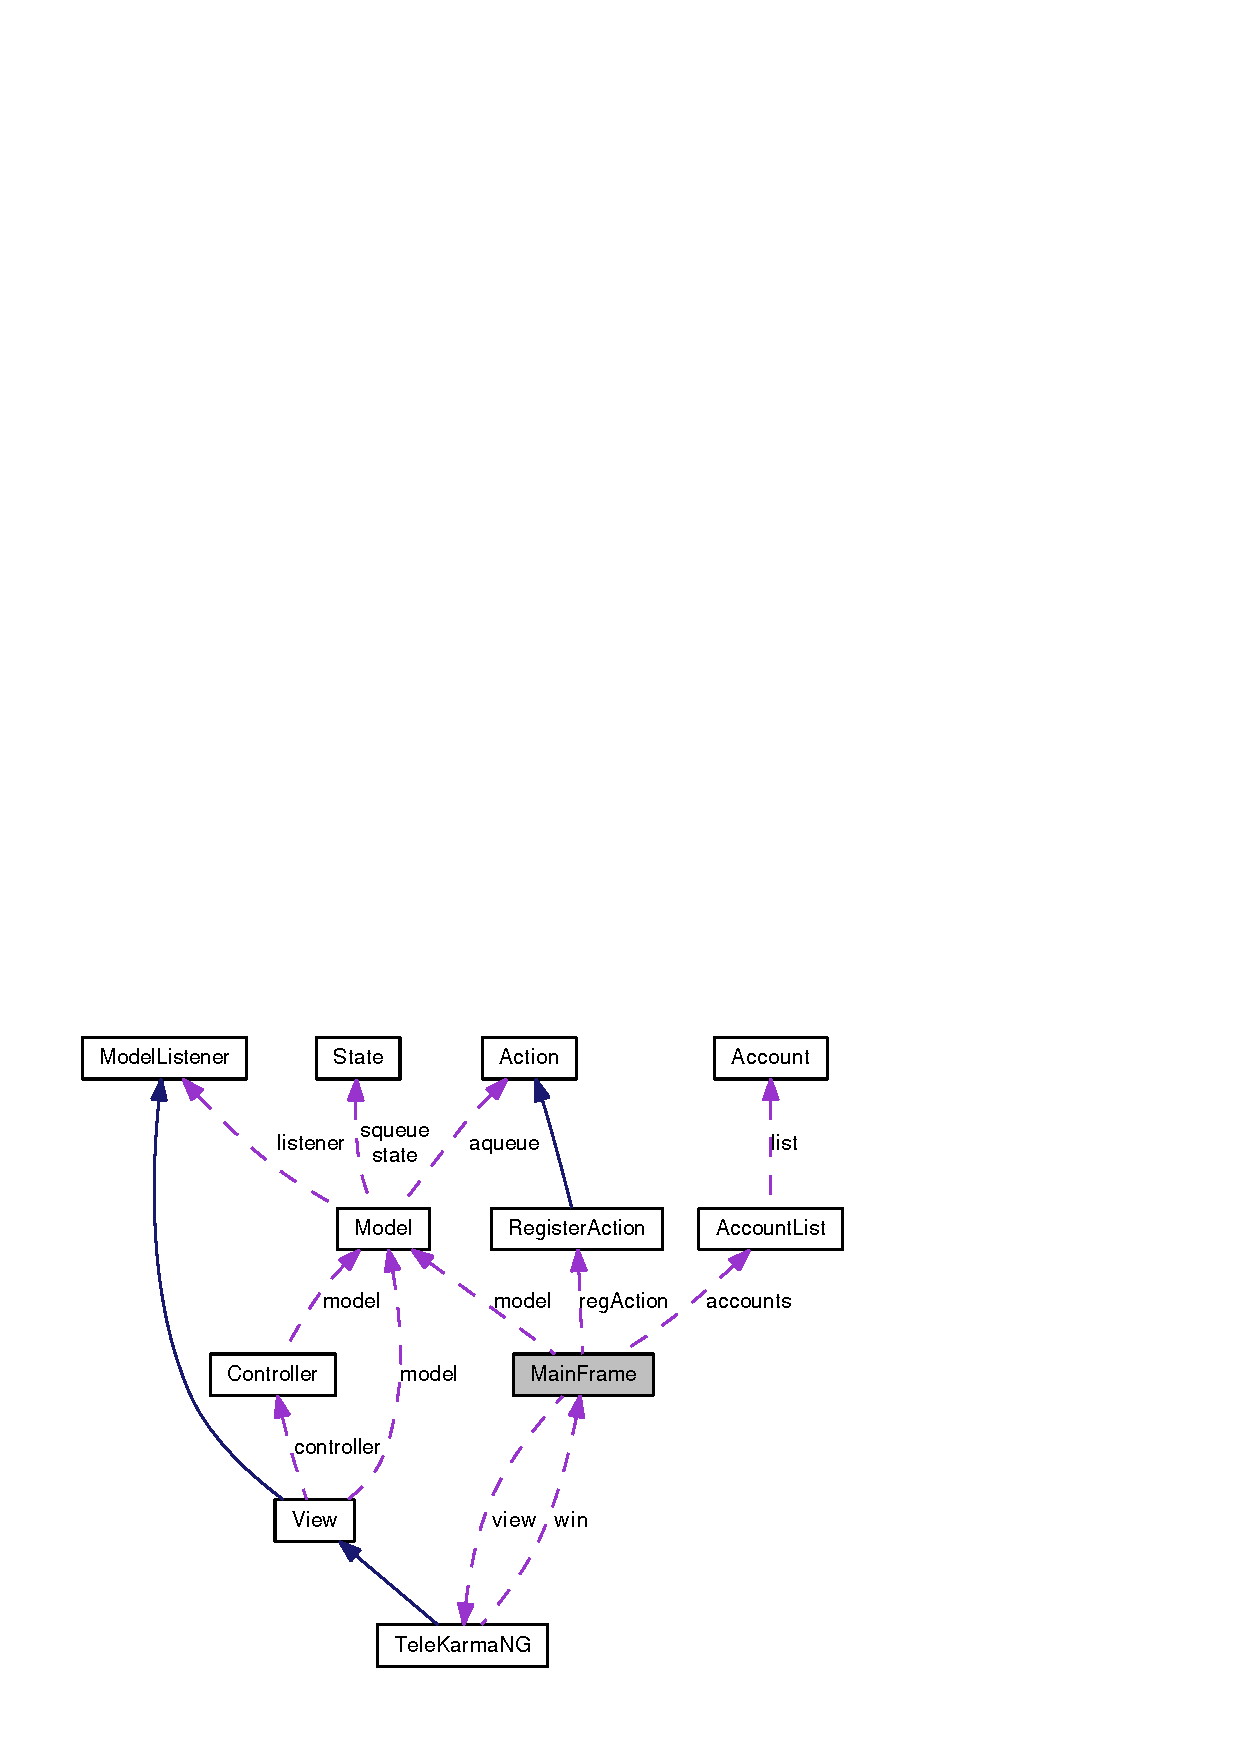
\includegraphics[width=400pt]{classMainFrame__coll__graph}
\end{center}
\end{figure}
\subsection*{Public Member Functions}
\begin{CompactItemize}
\item 
\hyperlink{classMainFrame_09f15beb9d0af78bd614358ad05b09f7}{MainFrame} (\hyperlink{classTeleKarmaNG}{TeleKarmaNG} $\ast$view, \hyperlink{classModel}{Model} $\ast$model, const wxString \&title, const wxPoint \&pos, const wxSize \&size)
\begin{CompactList}\small\item\em Constructs the main window. \item\end{CompactList}\item 
void \hyperlink{classMainFrame_5981c8c376f0b84971cd2f0574046ec7}{OnOpenRegisterDialog} (wxCommandEvent \&event)
\begin{CompactList}\small\item\em Handles registration initiation request. \item\end{CompactList}\item 
void \hyperlink{classMainFrame_330d1881b7c14a2d29235f3f437b0456}{OnOpenDialPad} (wxCommandEvent \&event)
\begin{CompactList}\small\item\em Handles opening of dial pad dialog. \item\end{CompactList}\item 
void \hyperlink{classMainFrame_b287a8d769abe22d71300beb96b14f03}{OnRegister} (const wxString \&s, const wxString \&r, const wxString \&u, const wxString \&p)
\begin{CompactList}\small\item\em Handles registration information submission. \item\end{CompactList}\item 
void \hyperlink{classMainFrame_6c21335bf2a3393f54b46889c8a559e5}{OnQuit} (wxCommandEvent \&event)
\begin{CompactList}\small\item\em Handles evExit (file-$>$exit). \item\end{CompactList}\item 
void \hyperlink{classMainFrame_9f6f7f89d8b9aded1334cfa6eaca22bc}{OnClose} (wxCloseEvent \&event)
\begin{CompactList}\small\item\em Handles system-prompted close events. \item\end{CompactList}\item 
void \hyperlink{classMainFrame_a6cb4bffa152fb2adad782a440af5de2}{OnAbout} (wxCommandEvent \&event)
\begin{CompactList}\small\item\em Handles evAbout. \item\end{CompactList}\item 
void \hyperlink{classMainFrame_5f4f33d38822481ad0608334a798325f}{OnStateChange} (\hyperlink{classwxStateChangeEvent}{wxStateChangeEvent} \&event)
\begin{CompactList}\small\item\em Responds to state changes. \item\end{CompactList}\item 
void \hyperlink{classMainFrame_90d32f36e1682ed4f5d2c2612ce6e2e3}{OnDial} (wxCommandEvent \&event)
\begin{CompactList}\small\item\em Dials. \item\end{CompactList}\item 
void \hyperlink{classMainFrame_dbb9352129402cc4595446460c80d09f}{OnHangUp} (wxCommandEvent \&event)
\begin{CompactList}\small\item\em Hangs Up. \item\end{CompactList}\item 
void \hyperlink{classMainFrame_343bfdcd2c0c3a32a58e11136408969b}{OnHold} (wxCommandEvent \&event)
\begin{CompactList}\small\item\em Place call on hold. \item\end{CompactList}\item 
void \hyperlink{classMainFrame_bcbd80572652cfe2bc9736704149d003}{OnAutoHold} (wxCommandEvent \&event)
\begin{CompactList}\small\item\em Place call on autohold. \item\end{CompactList}\item 
void \hyperlink{classMainFrame_cc537fb606070bc855356caef79efde8}{OnMuteAutoHold} (wxCommandEvent \&event)
\begin{CompactList}\small\item\em Place call on mute autohold. \item\end{CompactList}\item 
void \hyperlink{classMainFrame_0972eb674b39fe851271e432c2d0eb6c}{OnRetrieve} (wxCommandEvent \&event)
\begin{CompactList}\small\item\em Retrieve call from autohold. \item\end{CompactList}\item 
void \hyperlink{classMainFrame_a23ae1cbbe9db200b96285a46f23b6c3}{OnCloseRegisterDialog} (\hyperlink{classwxRegisterDialogClosedEvent}{wxRegisterDialogClosedEvent} \&event)
\begin{CompactList}\small\item\em Adjust to closure of register dialog. \item\end{CompactList}\item 
void \hyperlink{classMainFrame_c334df080d070c2f82c9457ad132ce18}{OnCloseDialPad} (\hyperlink{classwxDialPadClosedEvent}{wxDialPadClosedEvent} \&event)
\begin{CompactList}\small\item\em Adjust to closure of dial pad. \item\end{CompactList}\item 
void \hyperlink{classMainFrame_cf26ae04d239c8275ea85c5c4fc410e7}{OnAdjustControls} (const \hyperlink{state_8h_2c309f64131cbfdae6d95e6591f208e6}{StateID} state)
\begin{CompactList}\small\item\em Adjust the enabled/disabled states of controls. \item\end{CompactList}\item 
void \hyperlink{classMainFrame_f32b38c49c7276b789284ed9ee92a0c5}{Trace} (const wxString \&msg)
\begin{CompactList}\small\item\em Add a trace message to the console. \item\end{CompactList}\end{CompactItemize}


\subsection{Detailed Description}
The main window. 

\subsection{Constructor \& Destructor Documentation}
\hypertarget{classMainFrame_09f15beb9d0af78bd614358ad05b09f7}{
\index{MainFrame@{MainFrame}!MainFrame@{MainFrame}}
\index{MainFrame@{MainFrame}!MainFrame@{MainFrame}}
\subsubsection[{MainFrame}]{\setlength{\rightskip}{0pt plus 5cm}MainFrame::MainFrame ({\bf TeleKarmaNG} $\ast$ {\em view}, \/  {\bf Model} $\ast$ {\em model}, \/  const wxString \& {\em title}, \/  const wxPoint \& {\em pos}, \/  const wxSize \& {\em size})}}
\label{classMainFrame_09f15beb9d0af78bd614358ad05b09f7}


Constructs the main window. 



\subsection{Member Function Documentation}
\hypertarget{classMainFrame_a6cb4bffa152fb2adad782a440af5de2}{
\index{MainFrame@{MainFrame}!OnAbout@{OnAbout}}
\index{OnAbout@{OnAbout}!MainFrame@{MainFrame}}
\subsubsection[{OnAbout}]{\setlength{\rightskip}{0pt plus 5cm}void MainFrame::OnAbout (wxCommandEvent \& {\em event})}}
\label{classMainFrame_a6cb4bffa152fb2adad782a440af5de2}


Handles evAbout. 

\hypertarget{classMainFrame_cf26ae04d239c8275ea85c5c4fc410e7}{
\index{MainFrame@{MainFrame}!OnAdjustControls@{OnAdjustControls}}
\index{OnAdjustControls@{OnAdjustControls}!MainFrame@{MainFrame}}
\subsubsection[{OnAdjustControls}]{\setlength{\rightskip}{0pt plus 5cm}void MainFrame::OnAdjustControls (const {\bf StateID} {\em state})}}
\label{classMainFrame_cf26ae04d239c8275ea85c5c4fc410e7}


Adjust the enabled/disabled states of controls. 

\hypertarget{classMainFrame_bcbd80572652cfe2bc9736704149d003}{
\index{MainFrame@{MainFrame}!OnAutoHold@{OnAutoHold}}
\index{OnAutoHold@{OnAutoHold}!MainFrame@{MainFrame}}
\subsubsection[{OnAutoHold}]{\setlength{\rightskip}{0pt plus 5cm}void MainFrame::OnAutoHold (wxCommandEvent \& {\em event})}}
\label{classMainFrame_bcbd80572652cfe2bc9736704149d003}


Place call on autohold. 

\hypertarget{classMainFrame_9f6f7f89d8b9aded1334cfa6eaca22bc}{
\index{MainFrame@{MainFrame}!OnClose@{OnClose}}
\index{OnClose@{OnClose}!MainFrame@{MainFrame}}
\subsubsection[{OnClose}]{\setlength{\rightskip}{0pt plus 5cm}void MainFrame::OnClose (wxCloseEvent \& {\em event})}}
\label{classMainFrame_9f6f7f89d8b9aded1334cfa6eaca22bc}


Handles system-prompted close events. 

\hypertarget{classMainFrame_c334df080d070c2f82c9457ad132ce18}{
\index{MainFrame@{MainFrame}!OnCloseDialPad@{OnCloseDialPad}}
\index{OnCloseDialPad@{OnCloseDialPad}!MainFrame@{MainFrame}}
\subsubsection[{OnCloseDialPad}]{\setlength{\rightskip}{0pt plus 5cm}void MainFrame::OnCloseDialPad ({\bf wxDialPadClosedEvent} \& {\em event})}}
\label{classMainFrame_c334df080d070c2f82c9457ad132ce18}


Adjust to closure of dial pad. 

\hypertarget{classMainFrame_a23ae1cbbe9db200b96285a46f23b6c3}{
\index{MainFrame@{MainFrame}!OnCloseRegisterDialog@{OnCloseRegisterDialog}}
\index{OnCloseRegisterDialog@{OnCloseRegisterDialog}!MainFrame@{MainFrame}}
\subsubsection[{OnCloseRegisterDialog}]{\setlength{\rightskip}{0pt plus 5cm}void MainFrame::OnCloseRegisterDialog ({\bf wxRegisterDialogClosedEvent} \& {\em event})}}
\label{classMainFrame_a23ae1cbbe9db200b96285a46f23b6c3}


Adjust to closure of register dialog. 

\hypertarget{classMainFrame_90d32f36e1682ed4f5d2c2612ce6e2e3}{
\index{MainFrame@{MainFrame}!OnDial@{OnDial}}
\index{OnDial@{OnDial}!MainFrame@{MainFrame}}
\subsubsection[{OnDial}]{\setlength{\rightskip}{0pt plus 5cm}void MainFrame::OnDial (wxCommandEvent \& {\em event})}}
\label{classMainFrame_90d32f36e1682ed4f5d2c2612ce6e2e3}


Dials. 

\hypertarget{classMainFrame_dbb9352129402cc4595446460c80d09f}{
\index{MainFrame@{MainFrame}!OnHangUp@{OnHangUp}}
\index{OnHangUp@{OnHangUp}!MainFrame@{MainFrame}}
\subsubsection[{OnHangUp}]{\setlength{\rightskip}{0pt plus 5cm}void MainFrame::OnHangUp (wxCommandEvent \& {\em event})}}
\label{classMainFrame_dbb9352129402cc4595446460c80d09f}


Hangs Up. 

\hypertarget{classMainFrame_343bfdcd2c0c3a32a58e11136408969b}{
\index{MainFrame@{MainFrame}!OnHold@{OnHold}}
\index{OnHold@{OnHold}!MainFrame@{MainFrame}}
\subsubsection[{OnHold}]{\setlength{\rightskip}{0pt plus 5cm}void MainFrame::OnHold (wxCommandEvent \& {\em event})}}
\label{classMainFrame_343bfdcd2c0c3a32a58e11136408969b}


Place call on hold. 

\hypertarget{classMainFrame_cc537fb606070bc855356caef79efde8}{
\index{MainFrame@{MainFrame}!OnMuteAutoHold@{OnMuteAutoHold}}
\index{OnMuteAutoHold@{OnMuteAutoHold}!MainFrame@{MainFrame}}
\subsubsection[{OnMuteAutoHold}]{\setlength{\rightskip}{0pt plus 5cm}void MainFrame::OnMuteAutoHold (wxCommandEvent \& {\em event})}}
\label{classMainFrame_cc537fb606070bc855356caef79efde8}


Place call on mute autohold. 

\hypertarget{classMainFrame_330d1881b7c14a2d29235f3f437b0456}{
\index{MainFrame@{MainFrame}!OnOpenDialPad@{OnOpenDialPad}}
\index{OnOpenDialPad@{OnOpenDialPad}!MainFrame@{MainFrame}}
\subsubsection[{OnOpenDialPad}]{\setlength{\rightskip}{0pt plus 5cm}void MainFrame::OnOpenDialPad (wxCommandEvent \& {\em event})}}
\label{classMainFrame_330d1881b7c14a2d29235f3f437b0456}


Handles opening of dial pad dialog. 

\hypertarget{classMainFrame_5981c8c376f0b84971cd2f0574046ec7}{
\index{MainFrame@{MainFrame}!OnOpenRegisterDialog@{OnOpenRegisterDialog}}
\index{OnOpenRegisterDialog@{OnOpenRegisterDialog}!MainFrame@{MainFrame}}
\subsubsection[{OnOpenRegisterDialog}]{\setlength{\rightskip}{0pt plus 5cm}void MainFrame::OnOpenRegisterDialog (wxCommandEvent \& {\em event})}}
\label{classMainFrame_5981c8c376f0b84971cd2f0574046ec7}


Handles registration initiation request. 

\hypertarget{classMainFrame_6c21335bf2a3393f54b46889c8a559e5}{
\index{MainFrame@{MainFrame}!OnQuit@{OnQuit}}
\index{OnQuit@{OnQuit}!MainFrame@{MainFrame}}
\subsubsection[{OnQuit}]{\setlength{\rightskip}{0pt plus 5cm}void MainFrame::OnQuit (wxCommandEvent \& {\em event})}}
\label{classMainFrame_6c21335bf2a3393f54b46889c8a559e5}


Handles evExit (file-$>$exit). 

\hypertarget{classMainFrame_b287a8d769abe22d71300beb96b14f03}{
\index{MainFrame@{MainFrame}!OnRegister@{OnRegister}}
\index{OnRegister@{OnRegister}!MainFrame@{MainFrame}}
\subsubsection[{OnRegister}]{\setlength{\rightskip}{0pt plus 5cm}void MainFrame::OnRegister (const wxString \& {\em s}, \/  const wxString \& {\em r}, \/  const wxString \& {\em u}, \/  const wxString \& {\em p})}}
\label{classMainFrame_b287a8d769abe22d71300beb96b14f03}


Handles registration information submission. 

\hypertarget{classMainFrame_0972eb674b39fe851271e432c2d0eb6c}{
\index{MainFrame@{MainFrame}!OnRetrieve@{OnRetrieve}}
\index{OnRetrieve@{OnRetrieve}!MainFrame@{MainFrame}}
\subsubsection[{OnRetrieve}]{\setlength{\rightskip}{0pt plus 5cm}void MainFrame::OnRetrieve (wxCommandEvent \& {\em event})}}
\label{classMainFrame_0972eb674b39fe851271e432c2d0eb6c}


Retrieve call from autohold. 

\hypertarget{classMainFrame_5f4f33d38822481ad0608334a798325f}{
\index{MainFrame@{MainFrame}!OnStateChange@{OnStateChange}}
\index{OnStateChange@{OnStateChange}!MainFrame@{MainFrame}}
\subsubsection[{OnStateChange}]{\setlength{\rightskip}{0pt plus 5cm}void MainFrame::OnStateChange ({\bf wxStateChangeEvent} \& {\em event})}}
\label{classMainFrame_5f4f33d38822481ad0608334a798325f}


Responds to state changes. 

\hypertarget{classMainFrame_f32b38c49c7276b789284ed9ee92a0c5}{
\index{MainFrame@{MainFrame}!Trace@{Trace}}
\index{Trace@{Trace}!MainFrame@{MainFrame}}
\subsubsection[{Trace}]{\setlength{\rightskip}{0pt plus 5cm}void MainFrame::Trace (const wxString \& {\em msg})}}
\label{classMainFrame_f32b38c49c7276b789284ed9ee92a0c5}


Add a trace message to the console. 



The documentation for this class was generated from the following files:\begin{CompactItemize}
\item 
\hyperlink{gui_8h}{gui.h}\item 
\hyperlink{gui_8cpp}{gui.cpp}\end{CompactItemize}

\hypertarget{classModel}{
\section{Model Class Reference}
\label{classModel}\index{Model@{Model}}
}
{\tt \#include $<$model.h$>$}

Collaboration diagram for Model:\nopagebreak
\begin{figure}[H]
\begin{center}
\leavevmode
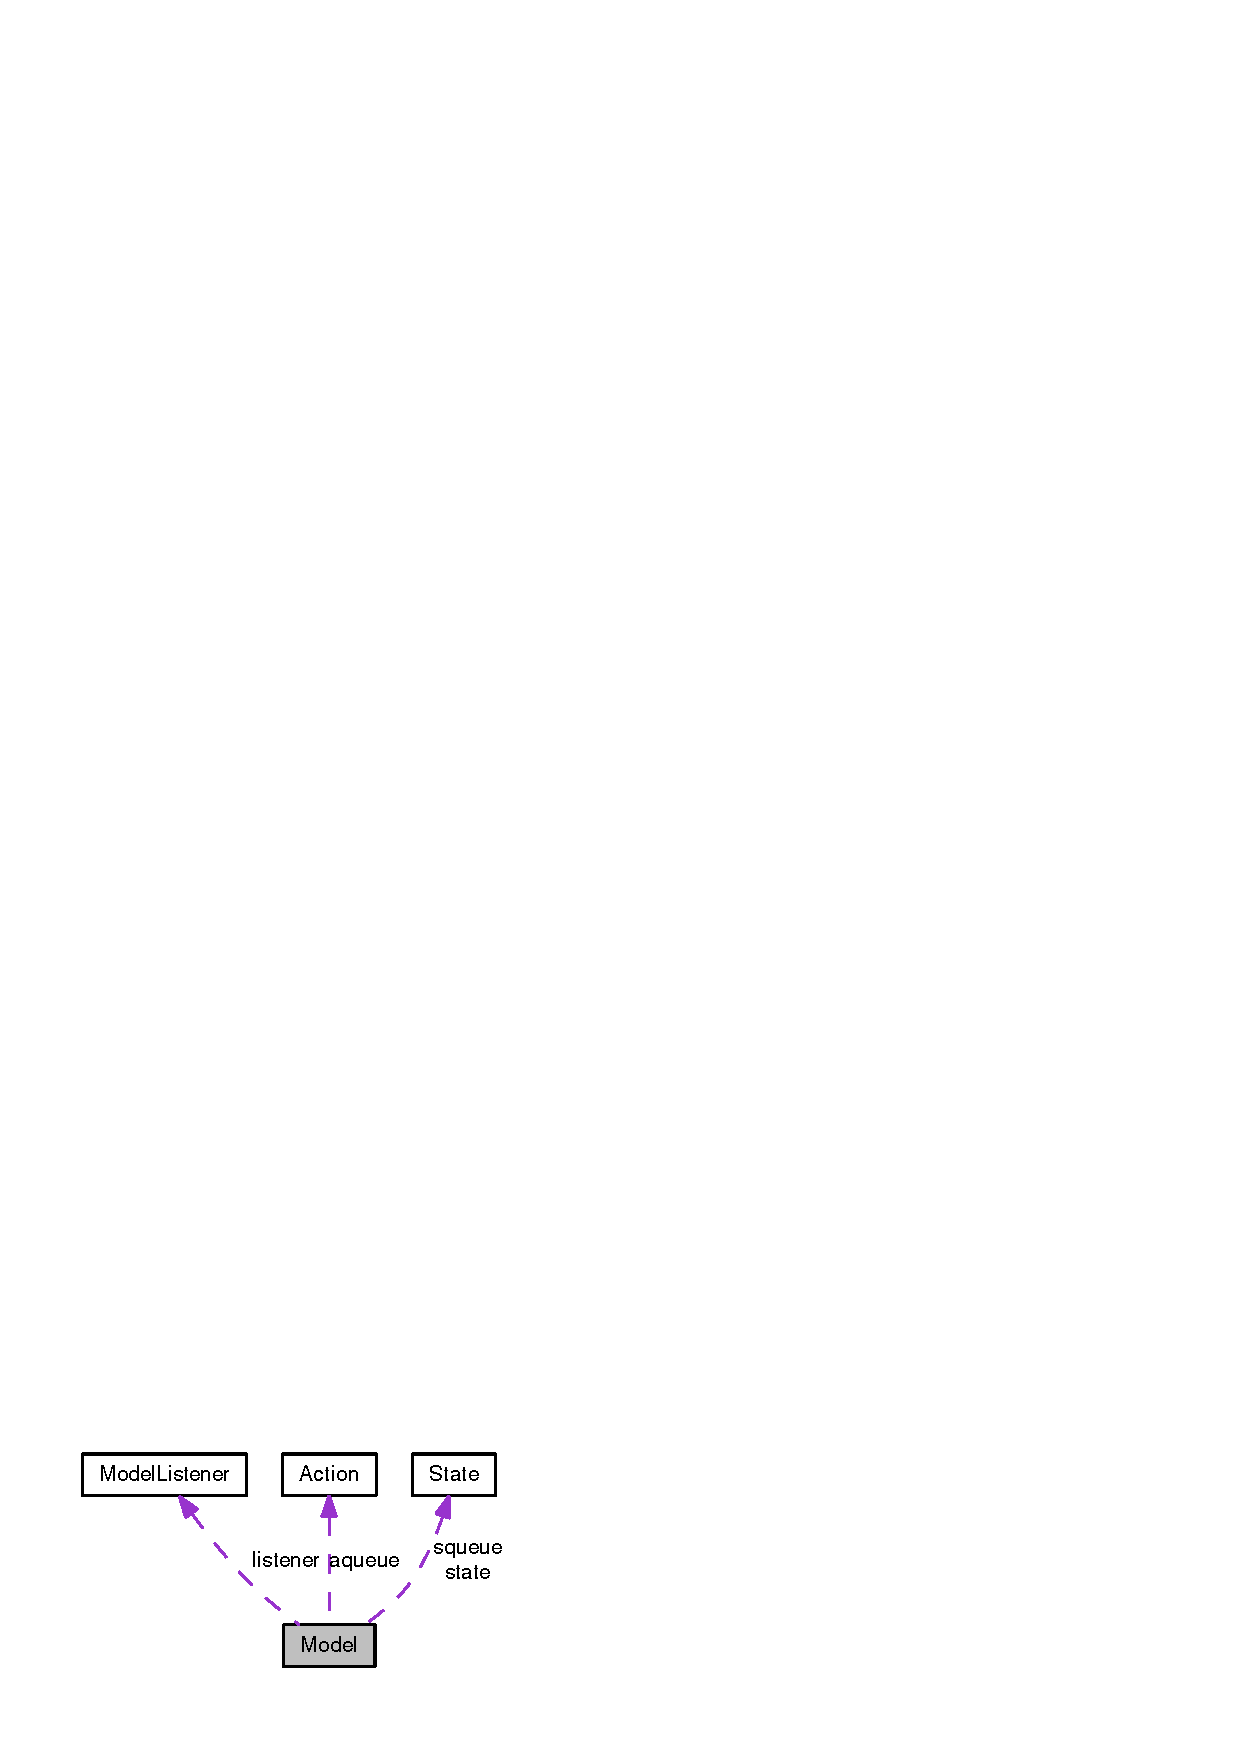
\includegraphics[width=245pt]{classModel__coll__graph}
\end{center}
\end{figure}
\subsection*{Public Member Functions}
\begin{CompactItemize}
\item 
\hyperlink{classModel_e3b375de5f6df4faf74a95d64748e048}{Model} ()
\begin{CompactList}\small\item\em Default constructor. \item\end{CompactList}\item 
\hyperlink{classModel_0dfa7627123dd65d7593b72cf03901f9}{Model} (int queueSize)
\begin{CompactList}\small\item\em Optional constructor. \item\end{CompactList}\item 
virtual \hyperlink{classModel_d6ebd2062a0b823db841a0b88baac4c0}{$\sim$Model} ()
\item 
virtual bool \hyperlink{classModel_1273906325b572fe38cc3c74c8f0f831}{EnqueueAction} (\hyperlink{classAction}{Action} $\ast$action)
\item 
virtual \hyperlink{classAction}{Action} $\ast$ \hyperlink{classModel_49c672e91b844a13b8cbee1d2382a5b4}{DequeueAction} ()
\item 
virtual \hyperlink{classState}{State} $\ast$ \hyperlink{classModel_a92abd0332df9f768033423b0cd8b3ae}{DequeueState} ()
\item 
virtual \hyperlink{classState}{State} $\ast$ \hyperlink{classModel_aca96bcd2e019aad9c4d4d7203b77cce}{GetState} ()
\item 
virtual bool \hyperlink{classModel_8b2d324213cf67b2e139144a25c6e3c3}{SetState} (\hyperlink{classState}{State} $\ast$newState)
\item 
virtual void \hyperlink{classModel_dca495055a5153c982891398d016e22d}{SetListener} (\hyperlink{classModelListener}{ModelListener} $\ast$l)
\item 
virtual void \hyperlink{classModel_d45dc4b460f571d748905f1c19e88577}{SetStunServer} (const PString \&val)
\begin{CompactList}\small\item\em Sets the stun server address or hostname. \item\end{CompactList}\item 
virtual PString \hyperlink{classModel_8011462d91a258e49920db3b157c7af6}{GetStunServer} ()
\begin{CompactList}\small\item\em Returns the stun server address or hostname. \item\end{CompactList}\item 
virtual void \hyperlink{classModel_d2fd66a01c2cea8bc295567da8998733}{SetStunType} (const PString \&val)
\begin{CompactList}\small\item\em Sets the stun server type description. \item\end{CompactList}\item 
virtual PString \hyperlink{classModel_6c040c5501c12f31f260280ea872b0b4}{GetStunType} ()
\begin{CompactList}\small\item\em Returns the stun server type description. \item\end{CompactList}\item 
virtual void \hyperlink{classModel_437d34289432b9687d0bc2f65d89aa4f}{SetRegistrar} (const PString \&val)
\begin{CompactList}\small\item\em Sets the SIP server address or hostname. \item\end{CompactList}\item 
virtual PString \hyperlink{classModel_5d7dd928f54ce00e04f1763728b9b85a}{GetRegistrar} ()
\begin{CompactList}\small\item\em Returns the stun server type description. \item\end{CompactList}\item 
virtual void \hyperlink{classModel_de7353a1170fbb7f587c069270be7f7a}{SetUserName} (const PString \&val)
\begin{CompactList}\small\item\em Sets the user name. \item\end{CompactList}\item 
virtual PString \hyperlink{classModel_18c1848740876abd9544c870c6665879}{GetUserName} ()
\begin{CompactList}\small\item\em Returns the user name. \item\end{CompactList}\item 
virtual void \hyperlink{classModel_e9a19897ea5d7d2417085a5d3a2a2f72}{SetDestination} (const PString \&val)
\begin{CompactList}\small\item\em Sets the call destination. \item\end{CompactList}\item 
virtual PString \hyperlink{classModel_b4354c982ea5543a43f9dfc0874ece20}{GetDestination} ()
\begin{CompactList}\small\item\em Returns the most recent call destination. \item\end{CompactList}\item 
virtual \hyperlink{classAccountList}{AccountList} $\ast$ \hyperlink{classModel_a0be0a124810faa919249d9a51bde1f4}{GetAccountList} (const PString \&fname)
\begin{CompactList}\small\item\em Returns a pointer to an \hyperlink{classAccountList}{AccountList} object attached to the given file. \item\end{CompactList}\end{CompactItemize}


\subsection{Detailed Description}
The \hyperlink{classTeleKarma}{TeleKarma} NG \hyperlink{classModel}{Model} superclass. 

The \hyperlink{classModel}{Model} holds system state and related data. Notably, the model stores the current state of the system, a queue of action requests generated by the \hyperlink{classView}{View} and a queue of error messages generated by the \hyperlink{classController}{Controller}. 

The \hyperlink{classModel}{Model} is designed to be robust and easy to use in multithreaded environments. All mutable internal fields are protected by private mutexes to prevent reading of those fields in an inconsistent state. 

{\bf Memory Management} 

It is critically important for developers utilizing methods of this class to read and understand the documentation for each method used. Method documentation discusses the caller's memory management responsibilities. These responsibilities vary depending on which method is being used. 

{\bf Thread Safety} 

This class is thread-safe when used properly. Extend this class with great care to preserve its thread-safe attributes. This class is designed to share information between threads. This mission motivates a concurrency-aware design that makes a best effort to prevent concurrency errors. However, this class does not prevent all possible concurrency errors that are potentially associated with its use. Developers must read and understand the documentation associated with each method. 

{\bf Dependencies} 

All \hyperlink{classState}{State} classes must correctly implement a clone method that returns a pointer to a new and complete copy of the object. This method must never return a pointer to a copy of the object shared with another caller and must not retain a copy of the pointer returned.  

\subsection{Constructor \& Destructor Documentation}
\hypertarget{classModel_e3b375de5f6df4faf74a95d64748e048}{
\index{Model@{Model}!Model@{Model}}
\index{Model@{Model}!Model@{Model}}
\subsubsection[{Model}]{\setlength{\rightskip}{0pt plus 5cm}Model::Model ()}}
\label{classModel_e3b375de5f6df4faf74a95d64748e048}


Default constructor. 

Creates a model with action and error message queues of fixed size equal to \hyperlink{model_8h_142810068f1b99cd93d3fc9f0e160e02}{QUEUE\_\-SIZE}. \hypertarget{classModel_0dfa7627123dd65d7593b72cf03901f9}{
\index{Model@{Model}!Model@{Model}}
\index{Model@{Model}!Model@{Model}}
\subsubsection[{Model}]{\setlength{\rightskip}{0pt plus 5cm}Model::Model (int {\em queueSize})}}
\label{classModel_0dfa7627123dd65d7593b72cf03901f9}


Optional constructor. 

Creates a model with action and error message queues of fixed size specified by the caller using the queueSize parameter. \begin{Desc}
\item[Parameters:]
\begin{description}
\item[{\em queueSize}]how big to make the queues. \end{description}
\end{Desc}
\hypertarget{classModel_d6ebd2062a0b823db841a0b88baac4c0}{
\index{Model@{Model}!$\sim$Model@{$\sim$Model}}
\index{$\sim$Model@{$\sim$Model}!Model@{Model}}
\subsubsection[{$\sim$Model}]{\setlength{\rightskip}{0pt plus 5cm}Model::$\sim$Model ()\hspace{0.3cm}{\tt  \mbox{[}virtual\mbox{]}}}}
\label{classModel_d6ebd2062a0b823db841a0b88baac4c0}


Virtual destructor. Deallocates: \begin{enumerate}
\item All internally allocated memory. \item The memory allocated to the current state. \item The memory allocated to any \hyperlink{classAction}{Action} objects remaining in the action queue. \item The memory allocated to any error messages remaining in the error message queue. \end{enumerate}


\subsection{Member Function Documentation}
\hypertarget{classModel_49c672e91b844a13b8cbee1d2382a5b4}{
\index{Model@{Model}!DequeueAction@{DequeueAction}}
\index{DequeueAction@{DequeueAction}!Model@{Model}}
\subsubsection[{DequeueAction}]{\setlength{\rightskip}{0pt plus 5cm}{\bf Action} $\ast$ Model::DequeueAction ()\hspace{0.3cm}{\tt  \mbox{[}virtual\mbox{]}}}}
\label{classModel_49c672e91b844a13b8cbee1d2382a5b4}


Dequeues and returns a pointer to an \hyperlink{classAction}{Action}. 

{\bf Memory Management} 

The caller assumes responsibility for deallocating the memory addressed by the pointer returned by this method. That memory should be deallocated using delete. The caller may deallocate the memory at a time of the caller's choosing. 

{\bf Thread Safety} 

This method is intended for use by a single consumer thread (the \hyperlink{classController}{Controller}). It may be used by multiple consumer threads without endangering built-in thread safety features. An enqueued pointer is never returned more than once, so multiple consumers cannot gain access to the same object solely by using this method. Callers must deallocate, and are free to modify, the memory addressed by the pointer returned by this method. Failure to adhere to these guidelines may defeat the thread safety features of this class. 

Override this method at your own risk!!  \begin{Desc}
\item[Returns:]a pointer to a previously enqueued \hyperlink{classAction}{Action} or NULL if the queue is empty. \end{Desc}
\hypertarget{classModel_a92abd0332df9f768033423b0cd8b3ae}{
\index{Model@{Model}!DequeueState@{DequeueState}}
\index{DequeueState@{DequeueState}!Model@{Model}}
\subsubsection[{DequeueState}]{\setlength{\rightskip}{0pt plus 5cm}{\bf State} $\ast$ Model::DequeueState ()\hspace{0.3cm}{\tt  \mbox{[}virtual\mbox{]}}}}
\label{classModel_a92abd0332df9f768033423b0cd8b3ae}


Dequeues and returns a pointer to a state. States are dequeued in the order they were set. 

{\bf Memory Management} 

The caller assumes responsibility for deallocating the memory addressed by the pointer returned by this method. That memory should be deallocated using delete. The caller may deallocate the memory at a time of the caller's choosing. 

{\bf Thread Safety} 

This method is intended for use by a single consumer thread (the \hyperlink{classView}{View}). It may be used by multiple consumer threads without endangering built-in thread safety features. An enqueued pointer is never returned more than once, so multiple consumers cannot gain access to the same object solely by using this method. Callers must deallocate, and are free to modify, the memory addressed by the pointer returned by this method. Failure to adhere to these guidelines may defeat the thread safety features of this class. 

Override this method at your own risk!!  \begin{Desc}
\item[Returns:]a pointer to a previously enqueued state or NULL if the queue is empty. \end{Desc}
\hypertarget{classModel_1273906325b572fe38cc3c74c8f0f831}{
\index{Model@{Model}!EnqueueAction@{EnqueueAction}}
\index{EnqueueAction@{EnqueueAction}!Model@{Model}}
\subsubsection[{EnqueueAction}]{\setlength{\rightskip}{0pt plus 5cm}bool Model::EnqueueAction ({\bf Action} $\ast$ {\em action})\hspace{0.3cm}{\tt  \mbox{[}virtual\mbox{]}}}}
\label{classModel_1273906325b572fe38cc3c74c8f0f831}


Enqueues an action. 

{\bf Memory Management} 

This class assumes responsibility for deallocating the memory addressed by the action parameter if and only if this method returns true. The caller retains responsibility for deallocating the memory addressed by the action parameter if this method returns false, and is free to do so at a time of the caller's choosing. 

{\bf Thread Safety} 

This method is intended for use by a single producer thread (the \hyperlink{classView}{View}). It may be used by multiple producer threads without endangering its thread safety features. Callers {\bf must not modify or deallocate} the memory allocated to the pointer passed into this method after calling this method. The pointer passed into this method must be a pointer to memory on the heap. Failure to adhere to these guidelines may defeat the thread safety features of this class. 

This class stores the pointer passed to this method and may share that pointer with a consumer. This method does not make a copy the memory addressed by the pointer. 

Override this method at your own risk!!  \begin{Desc}
\item[Parameters:]
\begin{description}
\item[{\em action}]pointer to an \hyperlink{classAction}{Action} object on the heap. \end{description}
\end{Desc}
\begin{Desc}
\item[Returns:]false if the pointer cannot be enqueued because the queue is full; true otherwise. \end{Desc}
\hypertarget{classModel_a0be0a124810faa919249d9a51bde1f4}{
\index{Model@{Model}!GetAccountList@{GetAccountList}}
\index{GetAccountList@{GetAccountList}!Model@{Model}}
\subsubsection[{GetAccountList}]{\setlength{\rightskip}{0pt plus 5cm}{\bf AccountList} $\ast$ Model::GetAccountList (const PString \& {\em fname})\hspace{0.3cm}{\tt  \mbox{[}virtual\mbox{]}}}}
\label{classModel_a0be0a124810faa919249d9a51bde1f4}


Returns a pointer to an \hyperlink{classAccountList}{AccountList} object attached to the given file. 

Note that no concurrency support is provided - this method assumes one caller and one call. Caller is responsible for deleting the returned object. \begin{Desc}
\item[Parameters:]
\begin{description}
\item[{\em fname}]path to and name of file containing accounts. \end{description}
\end{Desc}
\begin{Desc}
\item[Returns:]an \hyperlink{classAccountList}{AccountList} with at least one \hyperlink{classAccount}{Account}. If the file does not exist or cannot be opened, the \hyperlink{classAccountList}{AccountList} will contain a single \hyperlink{classAccount}{Account} where all values are the empty string. \end{Desc}
\hypertarget{classModel_b4354c982ea5543a43f9dfc0874ece20}{
\index{Model@{Model}!GetDestination@{GetDestination}}
\index{GetDestination@{GetDestination}!Model@{Model}}
\subsubsection[{GetDestination}]{\setlength{\rightskip}{0pt plus 5cm}PString Model::GetDestination ()\hspace{0.3cm}{\tt  \mbox{[}virtual\mbox{]}}}}
\label{classModel_b4354c982ea5543a43f9dfc0874ece20}


Returns the most recent call destination. 

Makes a unique copy for the exclusive use of the caller. Caller is responsible for deleting the copy produced. \hypertarget{classModel_5d7dd928f54ce00e04f1763728b9b85a}{
\index{Model@{Model}!GetRegistrar@{GetRegistrar}}
\index{GetRegistrar@{GetRegistrar}!Model@{Model}}
\subsubsection[{GetRegistrar}]{\setlength{\rightskip}{0pt plus 5cm}PString Model::GetRegistrar ()\hspace{0.3cm}{\tt  \mbox{[}virtual\mbox{]}}}}
\label{classModel_5d7dd928f54ce00e04f1763728b9b85a}


Returns the stun server type description. 

Makes a unique copy for the exclusive use of the caller. Caller is responsible for deleting the copy produced. \hypertarget{classModel_aca96bcd2e019aad9c4d4d7203b77cce}{
\index{Model@{Model}!GetState@{GetState}}
\index{GetState@{GetState}!Model@{Model}}
\subsubsection[{GetState}]{\setlength{\rightskip}{0pt plus 5cm}{\bf State} $\ast$ Model::GetState ()\hspace{0.3cm}{\tt  \mbox{[}virtual\mbox{]}}}}
\label{classModel_aca96bcd2e019aad9c4d4d7203b77cce}


Returns a copy of the current \hyperlink{classState}{State} object. 

{\bf Memory Management} 

The caller assumes responsibility for deallocating the memory addressed by the pointer returned by this method. That memory should be deallocated using delete. The caller may deallocate the memory at a time of the caller's choosing. 

{\bf Thread Safety} 

This method makes a copy of the current \hyperlink{classState}{State} on the heap using that State's clone() method and returns a pointer to the copy. Provided that the \hyperlink{classState}{State} is implemented properly (see class overview documentation), it is not possible for two calls to this method to obtain a pointer to the same copy of a \hyperlink{classState}{State}. This assures thread safety outside of this method and relieves the caller of any responsibility for synchronizing access to the returned memory block.  \begin{Desc}
\item[Returns:]a pointer to a unique copy of the current \hyperlink{classState}{State} object or NULL if the current \hyperlink{classState}{State} is undefined. \end{Desc}
\hypertarget{classModel_8011462d91a258e49920db3b157c7af6}{
\index{Model@{Model}!GetStunServer@{GetStunServer}}
\index{GetStunServer@{GetStunServer}!Model@{Model}}
\subsubsection[{GetStunServer}]{\setlength{\rightskip}{0pt plus 5cm}PString Model::GetStunServer ()\hspace{0.3cm}{\tt  \mbox{[}virtual\mbox{]}}}}
\label{classModel_8011462d91a258e49920db3b157c7af6}


Returns the stun server address or hostname. 

Makes a unique copy for the exclusive use of the caller. Caller is responsible for deleting the copy produced. \hypertarget{classModel_6c040c5501c12f31f260280ea872b0b4}{
\index{Model@{Model}!GetStunType@{GetStunType}}
\index{GetStunType@{GetStunType}!Model@{Model}}
\subsubsection[{GetStunType}]{\setlength{\rightskip}{0pt plus 5cm}PString Model::GetStunType ()\hspace{0.3cm}{\tt  \mbox{[}virtual\mbox{]}}}}
\label{classModel_6c040c5501c12f31f260280ea872b0b4}


Returns the stun server type description. 

Makes a unique copy for the exclusive use of the caller. Caller is responsible for deleting the copy produced. \hypertarget{classModel_18c1848740876abd9544c870c6665879}{
\index{Model@{Model}!GetUserName@{GetUserName}}
\index{GetUserName@{GetUserName}!Model@{Model}}
\subsubsection[{GetUserName}]{\setlength{\rightskip}{0pt plus 5cm}PString Model::GetUserName ()\hspace{0.3cm}{\tt  \mbox{[}virtual\mbox{]}}}}
\label{classModel_18c1848740876abd9544c870c6665879}


Returns the user name. 

Makes a unique copy for the exclusive use of the caller. Caller is responsible for deleting the copy produced. \hypertarget{classModel_e9a19897ea5d7d2417085a5d3a2a2f72}{
\index{Model@{Model}!SetDestination@{SetDestination}}
\index{SetDestination@{SetDestination}!Model@{Model}}
\subsubsection[{SetDestination}]{\setlength{\rightskip}{0pt plus 5cm}void Model::SetDestination (const PString \& {\em val})\hspace{0.3cm}{\tt  \mbox{[}virtual\mbox{]}}}}
\label{classModel_e9a19897ea5d7d2417085a5d3a2a2f72}


Sets the call destination. 

Copies the provided value. No expectation of update upon disconnection, but set upon each dialing. \begin{Desc}
\item[Parameters:]
\begin{description}
\item[{\em val}]call destination. \end{description}
\end{Desc}
\hypertarget{classModel_dca495055a5153c982891398d016e22d}{
\index{Model@{Model}!SetListener@{SetListener}}
\index{SetListener@{SetListener}!Model@{Model}}
\subsubsection[{SetListener}]{\setlength{\rightskip}{0pt plus 5cm}void Model::SetListener ({\bf ModelListener} $\ast$ {\em l})\hspace{0.3cm}{\tt  \mbox{[}virtual\mbox{]}}}}
\label{classModel_dca495055a5153c982891398d016e22d}


Sets the sole listener class. The OnStateChange() method of this class will be called each time the state is updated using \hyperlink{classModel_8b2d324213cf67b2e139144a25c6e3c3}{SetState(State $\ast$)}.  \begin{Desc}
\item[Parameters:]
\begin{description}
\item[{\em l}]a listener class. \end{description}
\end{Desc}
\hypertarget{classModel_437d34289432b9687d0bc2f65d89aa4f}{
\index{Model@{Model}!SetRegistrar@{SetRegistrar}}
\index{SetRegistrar@{SetRegistrar}!Model@{Model}}
\subsubsection[{SetRegistrar}]{\setlength{\rightskip}{0pt plus 5cm}void Model::SetRegistrar (const PString \& {\em val})\hspace{0.3cm}{\tt  \mbox{[}virtual\mbox{]}}}}
\label{classModel_437d34289432b9687d0bc2f65d89aa4f}


Sets the SIP server address or hostname. 

Copies the provided value. \begin{Desc}
\item[Parameters:]
\begin{description}
\item[{\em val}]SIP server address or hostname. \end{description}
\end{Desc}
\hypertarget{classModel_8b2d324213cf67b2e139144a25c6e3c3}{
\index{Model@{Model}!SetState@{SetState}}
\index{SetState@{SetState}!Model@{Model}}
\subsubsection[{SetState}]{\setlength{\rightskip}{0pt plus 5cm}bool Model::SetState ({\bf State} $\ast$ {\em newState})\hspace{0.3cm}{\tt  \mbox{[}virtual\mbox{]}}}}
\label{classModel_8b2d324213cf67b2e139144a25c6e3c3}


Sets and enqueues the current state. 

{\bf Memory Management} 

This class assumes responsibility for deallocating the memory addressed by the pointer passed to this method. 

{\bf Thread Safety} 

Callers {\bf must not modify or deallocate} the memory allocated to the pointer passed into this method after calling this method. The pointer passed into this method must be a pointer to memory on the heap. Failure to adhere to these guidelines may defeat the thread safety features of this class. 

This class stores the pointer passed to this method and makes that pointer available via \hyperlink{classModel_aca96bcd2e019aad9c4d4d7203b77cce}{GetState()}. This call also invokes the clone() method of \hyperlink{classState}{State} to make a distinct copy of the state for the queue.  \begin{Desc}
\item[Parameters:]
\begin{description}
\item[{\em newState}]the new state. \end{description}
\end{Desc}
\begin{Desc}
\item[Returns:]if the new state was successfully enqueued; false indicates the current state was set but could not be enqueued (the state queue is full). \end{Desc}
\hypertarget{classModel_d45dc4b460f571d748905f1c19e88577}{
\index{Model@{Model}!SetStunServer@{SetStunServer}}
\index{SetStunServer@{SetStunServer}!Model@{Model}}
\subsubsection[{SetStunServer}]{\setlength{\rightskip}{0pt plus 5cm}void Model::SetStunServer (const PString \& {\em val})\hspace{0.3cm}{\tt  \mbox{[}virtual\mbox{]}}}}
\label{classModel_d45dc4b460f571d748905f1c19e88577}


Sets the stun server address or hostname. 

Copies the provided value. \begin{Desc}
\item[Parameters:]
\begin{description}
\item[{\em val}]stun server address or hostname. \end{description}
\end{Desc}
\hypertarget{classModel_d2fd66a01c2cea8bc295567da8998733}{
\index{Model@{Model}!SetStunType@{SetStunType}}
\index{SetStunType@{SetStunType}!Model@{Model}}
\subsubsection[{SetStunType}]{\setlength{\rightskip}{0pt plus 5cm}void Model::SetStunType (const PString \& {\em val})\hspace{0.3cm}{\tt  \mbox{[}virtual\mbox{]}}}}
\label{classModel_d2fd66a01c2cea8bc295567da8998733}


Sets the stun server type description. 

Copies the provided value. \begin{Desc}
\item[Parameters:]
\begin{description}
\item[{\em val}]stun server type description. \end{description}
\end{Desc}
\hypertarget{classModel_de7353a1170fbb7f587c069270be7f7a}{
\index{Model@{Model}!SetUserName@{SetUserName}}
\index{SetUserName@{SetUserName}!Model@{Model}}
\subsubsection[{SetUserName}]{\setlength{\rightskip}{0pt plus 5cm}void Model::SetUserName (const PString \& {\em val})\hspace{0.3cm}{\tt  \mbox{[}virtual\mbox{]}}}}
\label{classModel_de7353a1170fbb7f587c069270be7f7a}


Sets the user name. 

Copies the provided value. \begin{Desc}
\item[Parameters:]
\begin{description}
\item[{\em val}]user name. \end{description}
\end{Desc}


The documentation for this class was generated from the following files:\begin{CompactItemize}
\item 
\hyperlink{model_8h}{model.h}\item 
\hyperlink{model_8cpp}{model.cpp}\end{CompactItemize}

\hypertarget{classModelListener}{
\section{ModelListener Class Reference}
\label{classModelListener}\index{ModelListener@{ModelListener}}
}
{\tt \#include $<$model.h$>$}

Inheritance diagram for ModelListener:\nopagebreak
\begin{figure}[H]
\begin{center}
\leavevmode

\includegraphics[width=198pt]{classModelListener__inherit__graph}
\end{center}
\end{figure}
\subsection*{Public Member Functions}
\begin{CompactItemize}
\item 
virtual void \hyperlink{classModelListener_63070a6f75480904846b7cfc6389aa4c}{OnStateChange} ()=0
\begin{CompactList}\small\item\em Abstract method gets called when \hyperlink{classModel_8b2d324213cf67b2e139144a25c6e3c3}{Model::SetState(State $\ast$)} is called. \item\end{CompactList}\end{CompactItemize}


\subsection{Detailed Description}
Interface for a class that can register itself with the \hyperlink{classModel}{Model} for notification upon state changes.  

\subsection{Member Function Documentation}
\hypertarget{classModelListener_63070a6f75480904846b7cfc6389aa4c}{
\index{ModelListener@{ModelListener}!OnStateChange@{OnStateChange}}
\index{OnStateChange@{OnStateChange}!ModelListener@{ModelListener}}
\subsubsection[{OnStateChange}]{\setlength{\rightskip}{0pt plus 5cm}virtual void ModelListener::OnStateChange ()\hspace{0.3cm}{\tt  \mbox{[}pure virtual\mbox{]}}}}
\label{classModelListener_63070a6f75480904846b7cfc6389aa4c}


Abstract method gets called when \hyperlink{classModel_8b2d324213cf67b2e139144a25c6e3c3}{Model::SetState(State $\ast$)} is called. 



Implemented in \hyperlink{classTeleKarmaNG_ce1e8d62f3e1d586e2aa5d2012c9a766}{TeleKarmaNG}, and \hyperlink{classView_92a0d9fd64b52e7f85d45c46c28a6546}{View}.

The documentation for this class was generated from the following file:\begin{CompactItemize}
\item 
\hyperlink{model_8h}{model.h}\end{CompactItemize}

\hypertarget{classPlaySoundAction}{
\section{PlaySoundAction Class Reference}
\label{classPlaySoundAction}\index{PlaySoundAction@{PlaySoundAction}}
}
{\tt \#include $<$action.h$>$}

Inheritance diagram for PlaySoundAction:\nopagebreak
\begin{figure}[H]
\begin{center}
\leavevmode

\includegraphics[width=136pt]{classPlaySoundAction__inherit__graph}
\end{center}
\end{figure}
Collaboration diagram for PlaySoundAction:\nopagebreak
\begin{figure}[H]
\begin{center}
\leavevmode

\includegraphics[width=136pt]{classPlaySoundAction__coll__graph}
\end{center}
\end{figure}
\subsection*{Public Member Functions}
\begin{CompactItemize}
\item 
\hyperlink{classPlaySoundAction_52a859c9276e8b94fc49dab724791ef2}{PlaySoundAction} (const PString \&\hyperlink{classPlaySoundAction_a79fe8c0c31676fff2718ff9b5fe031c}{fname}, int \hyperlink{classAction_51e5d56a6aa4a037e90df19587a225c7}{turn})
\end{CompactItemize}
\subsection*{Public Attributes}
\begin{CompactItemize}
\item 
const PString \hyperlink{classPlaySoundAction_a79fe8c0c31676fff2718ff9b5fe031c}{fname}
\end{CompactItemize}


\subsection{Constructor \& Destructor Documentation}
\hypertarget{classPlaySoundAction_52a859c9276e8b94fc49dab724791ef2}{
\index{PlaySoundAction@{PlaySoundAction}!PlaySoundAction@{PlaySoundAction}}
\index{PlaySoundAction@{PlaySoundAction}!PlaySoundAction@{PlaySoundAction}}
\subsubsection[{PlaySoundAction}]{\setlength{\rightskip}{0pt plus 5cm}PlaySoundAction::PlaySoundAction (const PString \& {\em fname}, \/  int {\em turn})\hspace{0.3cm}{\tt  \mbox{[}inline\mbox{]}}}}
\label{classPlaySoundAction_52a859c9276e8b94fc49dab724791ef2}




\subsection{Member Data Documentation}
\hypertarget{classPlaySoundAction_a79fe8c0c31676fff2718ff9b5fe031c}{
\index{PlaySoundAction@{PlaySoundAction}!fname@{fname}}
\index{fname@{fname}!PlaySoundAction@{PlaySoundAction}}
\subsubsection[{fname}]{\setlength{\rightskip}{0pt plus 5cm}const PString {\bf PlaySoundAction::fname}}}
\label{classPlaySoundAction_a79fe8c0c31676fff2718ff9b5fe031c}




The documentation for this class was generated from the following file:\begin{CompactItemize}
\item 
\hyperlink{action_8h}{action.h}\end{CompactItemize}

\hypertarget{classQuitAction}{
\section{QuitAction Class Reference}
\label{classQuitAction}\index{QuitAction@{QuitAction}}
}
{\tt \#include $<$action.h$>$}

Inheritance diagram for QuitAction:\nopagebreak
\begin{figure}[H]
\begin{center}
\leavevmode
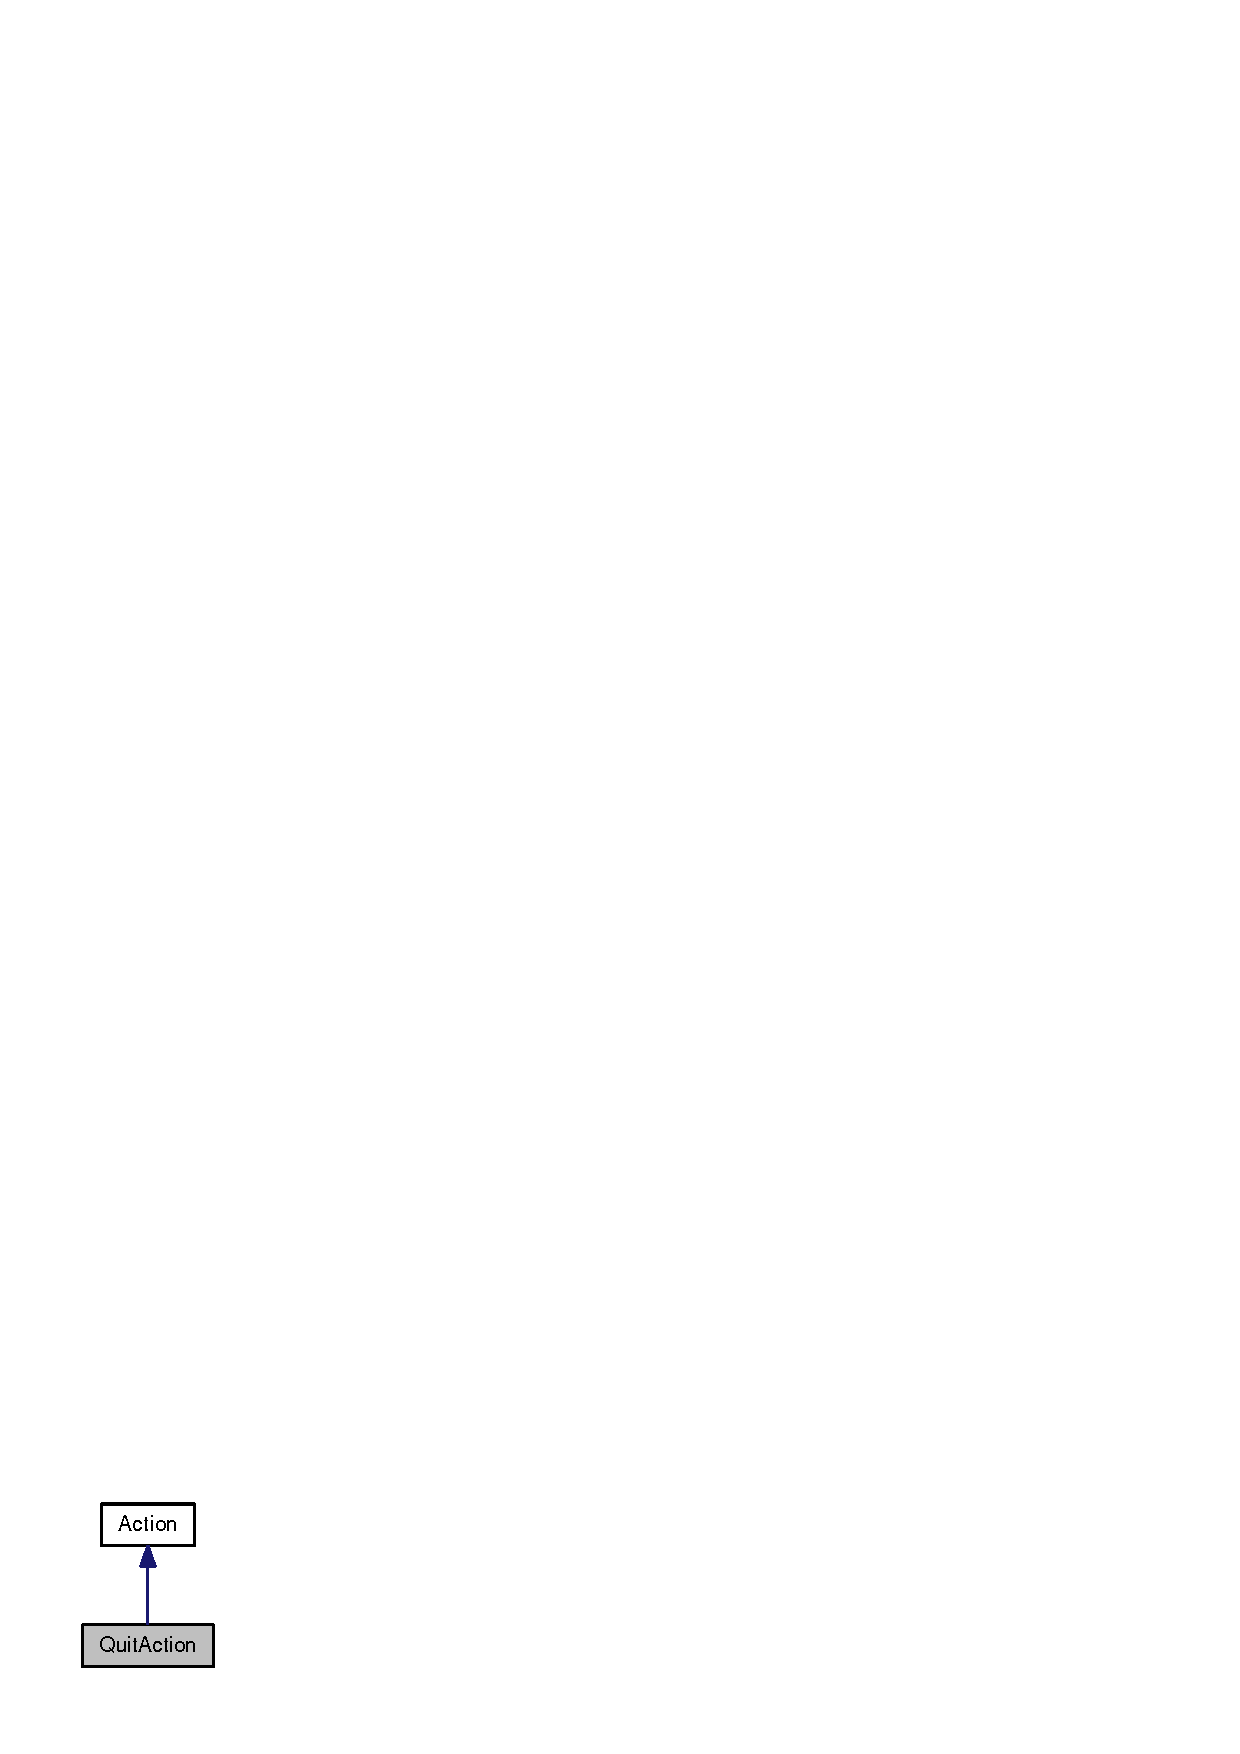
\includegraphics[width=106pt]{classQuitAction__inherit__graph}
\end{center}
\end{figure}
Collaboration diagram for QuitAction:\nopagebreak
\begin{figure}[H]
\begin{center}
\leavevmode
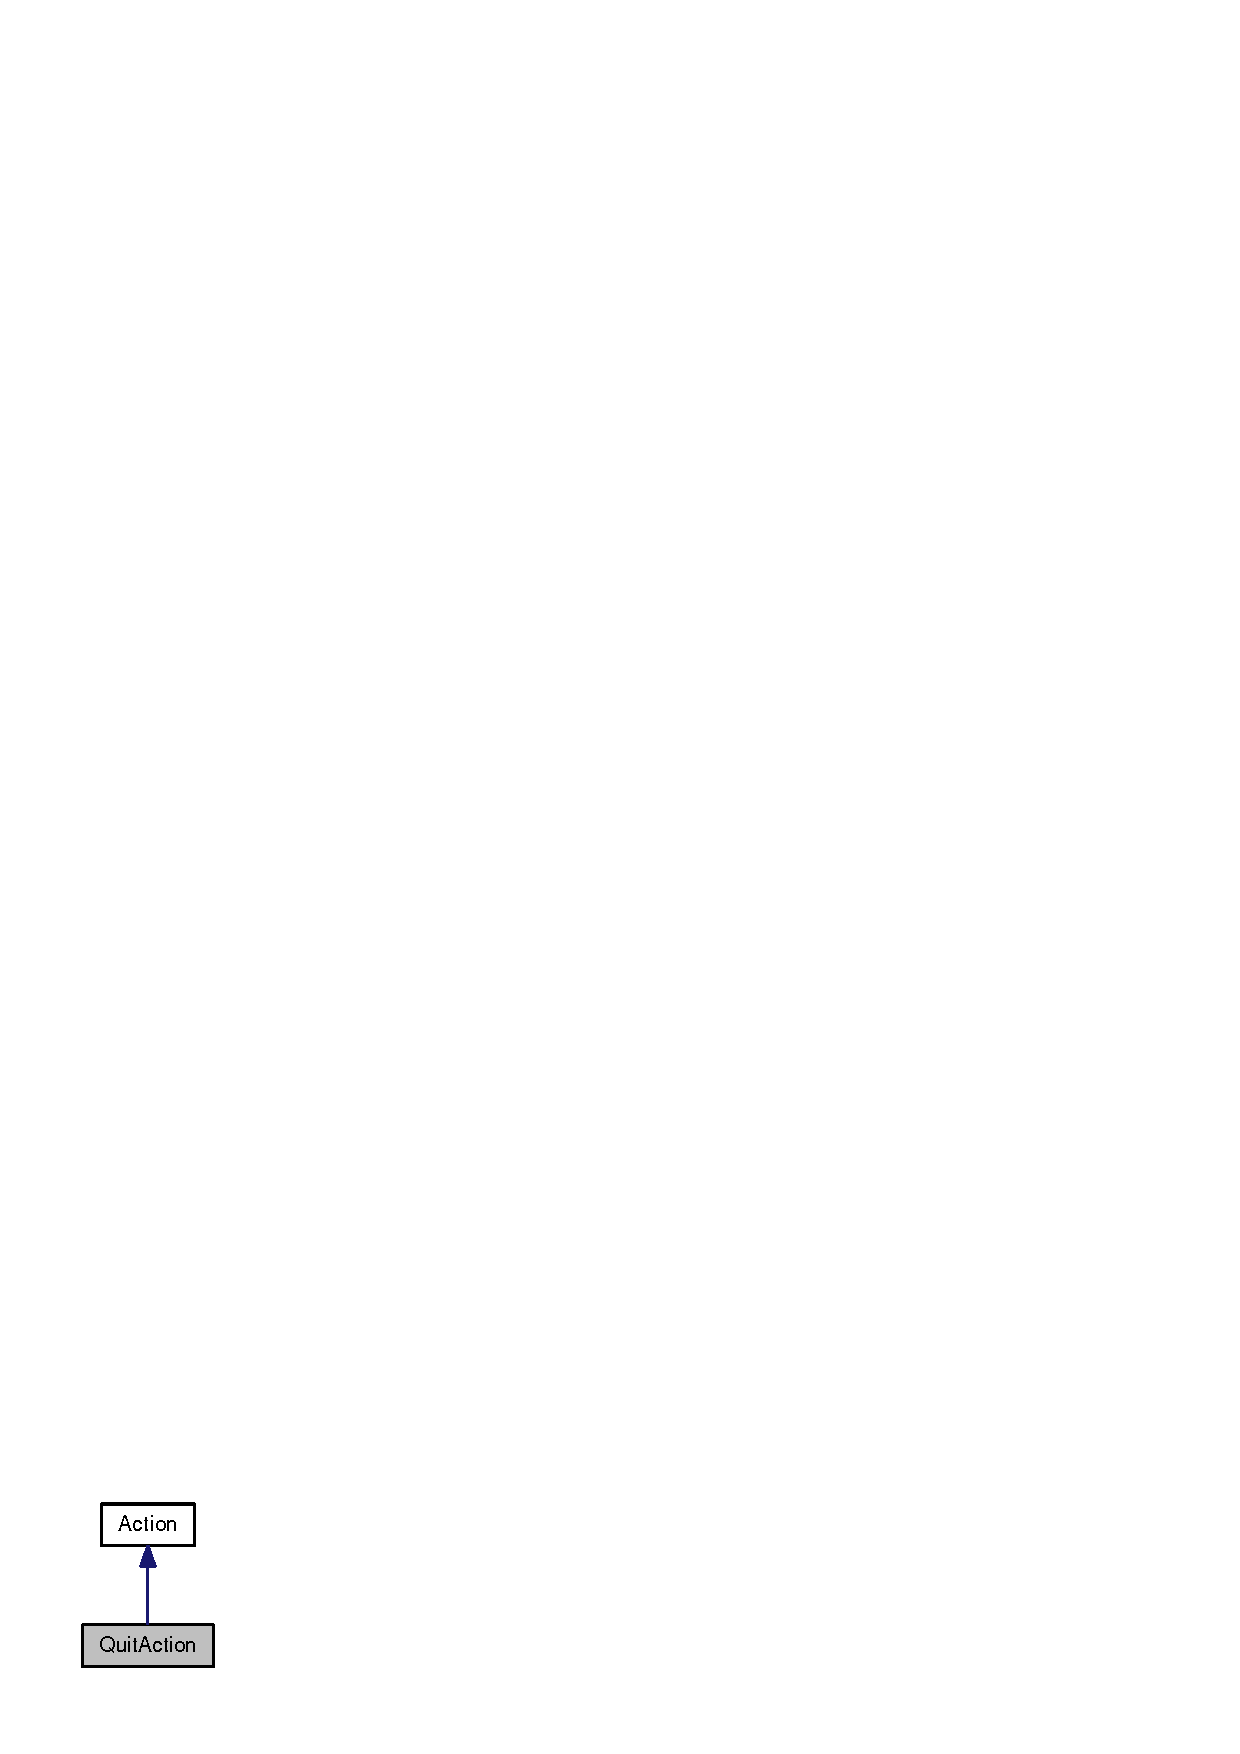
\includegraphics[width=106pt]{classQuitAction__coll__graph}
\end{center}
\end{figure}
\subsection*{Public Member Functions}
\begin{CompactItemize}
\item 
\hyperlink{classQuitAction_2289ac1a77e824192de8fd60b36d17e8}{QuitAction} (int \hyperlink{classAction_51e5d56a6aa4a037e90df19587a225c7}{turn})
\end{CompactItemize}


\subsection{Constructor \& Destructor Documentation}
\hypertarget{classQuitAction_2289ac1a77e824192de8fd60b36d17e8}{
\index{QuitAction@{QuitAction}!QuitAction@{QuitAction}}
\index{QuitAction@{QuitAction}!QuitAction@{QuitAction}}
\subsubsection[{QuitAction}]{\setlength{\rightskip}{0pt plus 5cm}QuitAction::QuitAction (int {\em turn})\hspace{0.3cm}{\tt  \mbox{[}inline\mbox{]}}}}
\label{classQuitAction_2289ac1a77e824192de8fd60b36d17e8}




The documentation for this class was generated from the following file:\begin{CompactItemize}
\item 
\hyperlink{action_8h}{action.h}\end{CompactItemize}

\hypertarget{classRegisterAction}{
\section{RegisterAction Class Reference}
\label{classRegisterAction}\index{RegisterAction@{RegisterAction}}
}
{\tt \#include $<$action.h$>$}

Inheritance diagram for RegisterAction:\nopagebreak
\begin{figure}[H]
\begin{center}
\leavevmode

\includegraphics[width=126pt]{classRegisterAction__inherit__graph}
\end{center}
\end{figure}
Collaboration diagram for RegisterAction:\nopagebreak
\begin{figure}[H]
\begin{center}
\leavevmode

\includegraphics[width=126pt]{classRegisterAction__coll__graph}
\end{center}
\end{figure}
\subsection*{Public Member Functions}
\begin{CompactItemize}
\item 
\hyperlink{classRegisterAction_955eec21894f1c59ad8e9692430476f9}{RegisterAction} (const PString \&\hyperlink{classRegisterAction_ac35a1ac2065a7114718b44d205ee8bd}{registrar}, const PString \&\hyperlink{classRegisterAction_aa4a6618f15066d50aec6d2a4b07d20f}{user}, const PString \&\hyperlink{classRegisterAction_55bb90773d5147d594f8601706a1bcc7}{password}, int \hyperlink{classAction_51e5d56a6aa4a037e90df19587a225c7}{turn})
\end{CompactItemize}
\subsection*{Public Attributes}
\begin{CompactItemize}
\item 
const PString \hyperlink{classRegisterAction_ac35a1ac2065a7114718b44d205ee8bd}{registrar}
\item 
const PString \hyperlink{classRegisterAction_aa4a6618f15066d50aec6d2a4b07d20f}{user}
\item 
const PString \hyperlink{classRegisterAction_55bb90773d5147d594f8601706a1bcc7}{password}
\end{CompactItemize}


\subsection{Constructor \& Destructor Documentation}
\hypertarget{classRegisterAction_955eec21894f1c59ad8e9692430476f9}{
\index{RegisterAction@{RegisterAction}!RegisterAction@{RegisterAction}}
\index{RegisterAction@{RegisterAction}!RegisterAction@{RegisterAction}}
\subsubsection[{RegisterAction}]{\setlength{\rightskip}{0pt plus 5cm}RegisterAction::RegisterAction (const PString \& {\em registrar}, \/  const PString \& {\em user}, \/  const PString \& {\em password}, \/  int {\em turn})}}
\label{classRegisterAction_955eec21894f1c59ad8e9692430476f9}




\subsection{Member Data Documentation}
\hypertarget{classRegisterAction_55bb90773d5147d594f8601706a1bcc7}{
\index{RegisterAction@{RegisterAction}!password@{password}}
\index{password@{password}!RegisterAction@{RegisterAction}}
\subsubsection[{password}]{\setlength{\rightskip}{0pt plus 5cm}const PString {\bf RegisterAction::password}}}
\label{classRegisterAction_55bb90773d5147d594f8601706a1bcc7}


\hypertarget{classRegisterAction_ac35a1ac2065a7114718b44d205ee8bd}{
\index{RegisterAction@{RegisterAction}!registrar@{registrar}}
\index{registrar@{registrar}!RegisterAction@{RegisterAction}}
\subsubsection[{registrar}]{\setlength{\rightskip}{0pt plus 5cm}const PString {\bf RegisterAction::registrar}}}
\label{classRegisterAction_ac35a1ac2065a7114718b44d205ee8bd}


\hypertarget{classRegisterAction_aa4a6618f15066d50aec6d2a4b07d20f}{
\index{RegisterAction@{RegisterAction}!user@{user}}
\index{user@{user}!RegisterAction@{RegisterAction}}
\subsubsection[{user}]{\setlength{\rightskip}{0pt plus 5cm}const PString {\bf RegisterAction::user}}}
\label{classRegisterAction_aa4a6618f15066d50aec6d2a4b07d20f}




The documentation for this class was generated from the following files:\begin{CompactItemize}
\item 
\hyperlink{action_8h}{action.h}\item 
\hyperlink{action_8cpp}{action.cpp}\end{CompactItemize}

\hypertarget{classRegisterDialog}{
\section{RegisterDialog Class Reference}
\label{classRegisterDialog}\index{RegisterDialog@{RegisterDialog}}
}
Modal registration dialog box.  


{\tt \#include $<$gui.h$>$}

Collaboration diagram for RegisterDialog:\nopagebreak
\begin{figure}[H]
\begin{center}
\leavevmode
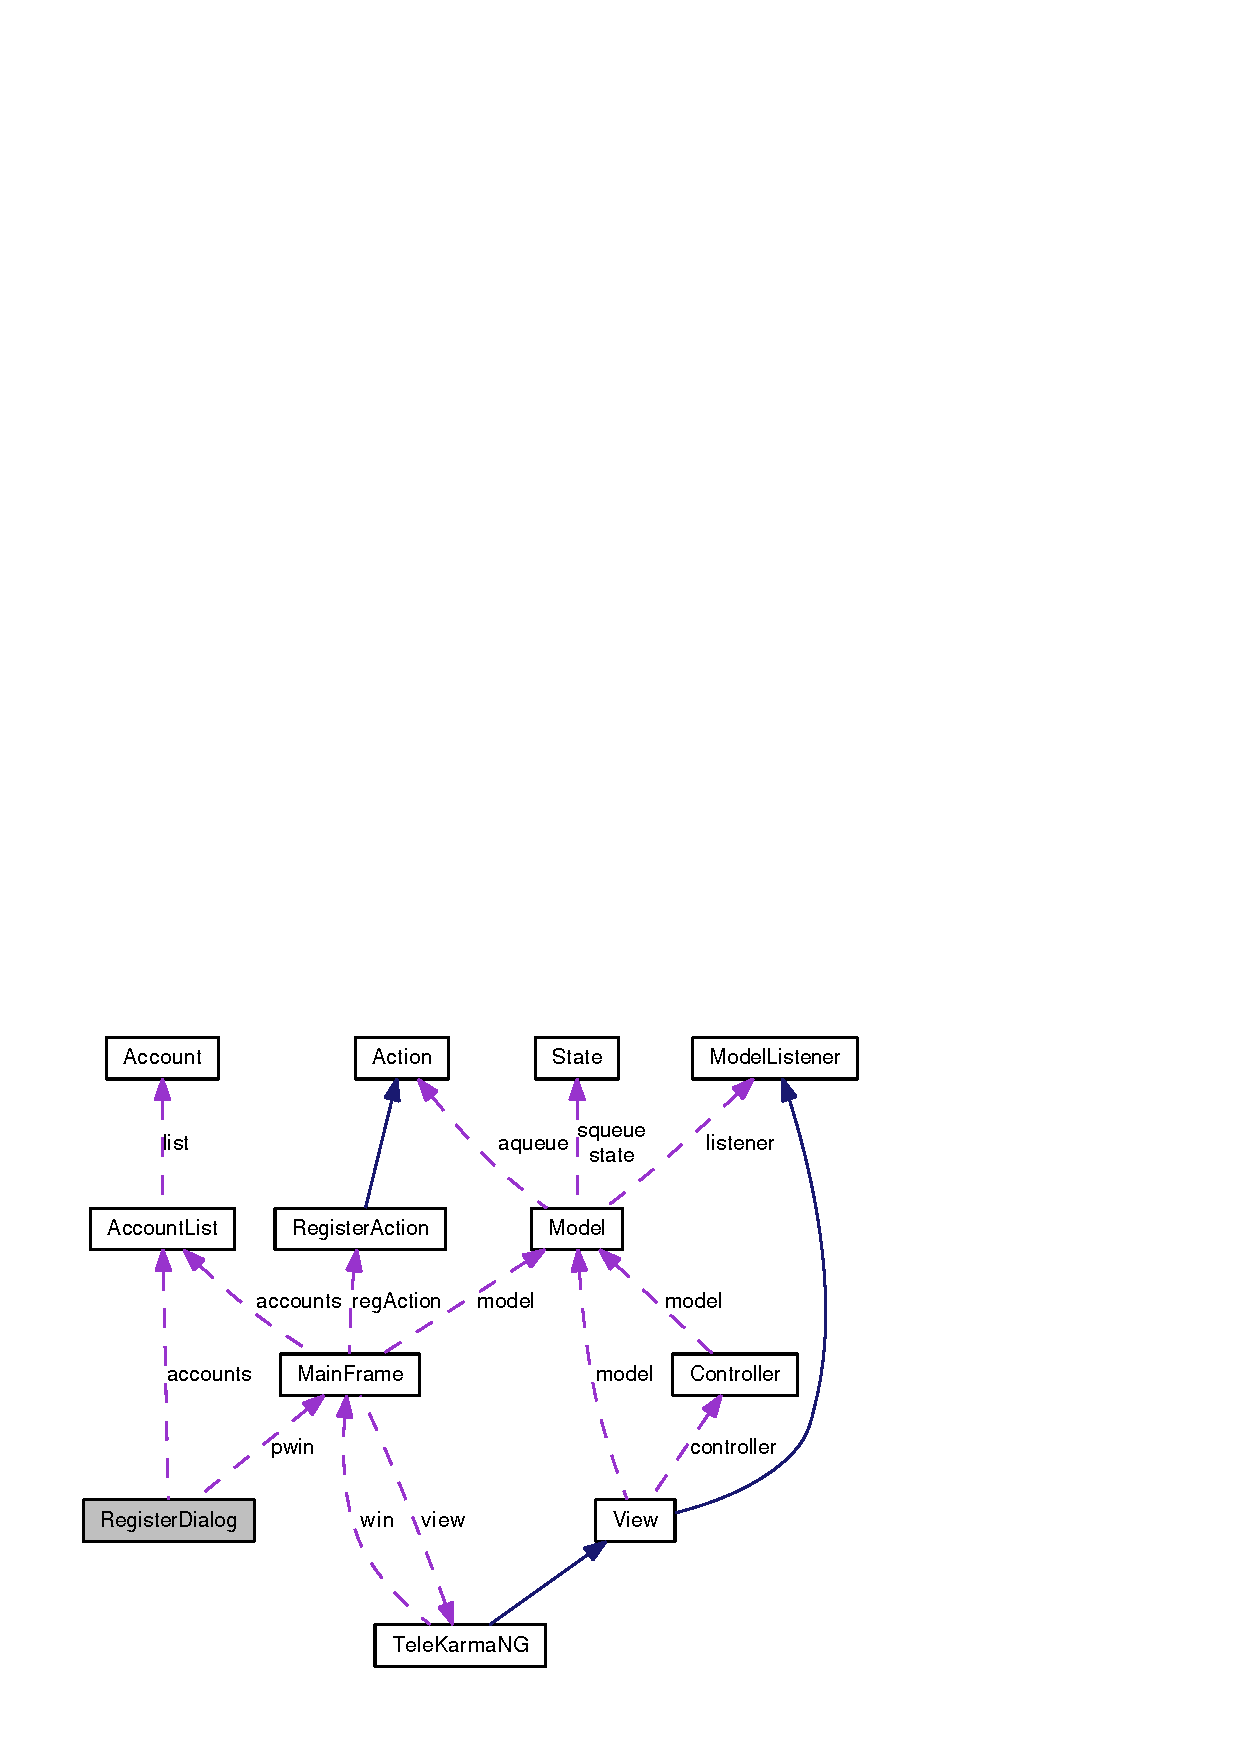
\includegraphics[width=400pt]{classRegisterDialog__coll__graph}
\end{center}
\end{figure}
\subsection*{Public Member Functions}
\begin{CompactItemize}
\item 
\hyperlink{classRegisterDialog_b07d91afc6ed60fd752ee324c322e2d8}{RegisterDialog} (\hyperlink{classMainFrame}{MainFrame} $\ast$pwin, \hyperlink{classAccountList}{AccountList} $\ast$accounts)
\begin{CompactList}\small\item\em Constructor. \item\end{CompactList}\item 
void \hyperlink{classRegisterDialog_6c95acf152a19de81ab996dcef977827}{OnClose} (wxCloseEvent \&event)
\begin{CompactList}\small\item\em Handles system-prompted close events. \item\end{CompactList}\item 
void \hyperlink{classRegisterDialog_334ccf10990ab1ec905088ea69187c2b}{OnRegister} (wxCommandEvent \&event)
\begin{CompactList}\small\item\em Initiates registration via pwin and closes the dialog. \item\end{CompactList}\item 
void \hyperlink{classRegisterDialog_3389f6b8e9ec03901de4f5424d8ea201}{OnCancel} (wxCommandEvent \&event)
\begin{CompactList}\small\item\em Closes this dialog when the cancel button is clicked. \item\end{CompactList}\end{CompactItemize}


\subsection{Detailed Description}
Modal registration dialog box. 



\subsection{Constructor \& Destructor Documentation}
\hypertarget{classRegisterDialog_b07d91afc6ed60fd752ee324c322e2d8}{
\index{RegisterDialog@{RegisterDialog}!RegisterDialog@{RegisterDialog}}
\index{RegisterDialog@{RegisterDialog}!RegisterDialog@{RegisterDialog}}
\subsubsection[{RegisterDialog}]{\setlength{\rightskip}{0pt plus 5cm}RegisterDialog::RegisterDialog ({\bf MainFrame} $\ast$ {\em pwin}, \/  {\bf AccountList} $\ast$ {\em accounts})}}
\label{classRegisterDialog_b07d91afc6ed60fd752ee324c322e2d8}


Constructor. 

\begin{Desc}
\item[Parameters:]
\begin{description}
\item[{\em pwin}]the parent window. \item[{\em accounts}]user's account list. \end{description}
\end{Desc}


\subsection{Member Function Documentation}
\hypertarget{classRegisterDialog_3389f6b8e9ec03901de4f5424d8ea201}{
\index{RegisterDialog@{RegisterDialog}!OnCancel@{OnCancel}}
\index{OnCancel@{OnCancel}!RegisterDialog@{RegisterDialog}}
\subsubsection[{OnCancel}]{\setlength{\rightskip}{0pt plus 5cm}void RegisterDialog::OnCancel (wxCommandEvent \& {\em event})}}
\label{classRegisterDialog_3389f6b8e9ec03901de4f5424d8ea201}


Closes this dialog when the cancel button is clicked. 

Notifies pwin. Exclusively for use by wxWidgets event dispatcher. \hypertarget{classRegisterDialog_6c95acf152a19de81ab996dcef977827}{
\index{RegisterDialog@{RegisterDialog}!OnClose@{OnClose}}
\index{OnClose@{OnClose}!RegisterDialog@{RegisterDialog}}
\subsubsection[{OnClose}]{\setlength{\rightskip}{0pt plus 5cm}void RegisterDialog::OnClose (wxCloseEvent \& {\em event})}}
\label{classRegisterDialog_6c95acf152a19de81ab996dcef977827}


Handles system-prompted close events. 

Notifies pwin. Exclusively for use by wxWidgets event dispatcher. \hypertarget{classRegisterDialog_334ccf10990ab1ec905088ea69187c2b}{
\index{RegisterDialog@{RegisterDialog}!OnRegister@{OnRegister}}
\index{OnRegister@{OnRegister}!RegisterDialog@{RegisterDialog}}
\subsubsection[{OnRegister}]{\setlength{\rightskip}{0pt plus 5cm}void RegisterDialog::OnRegister (wxCommandEvent \& {\em event})}}
\label{classRegisterDialog_334ccf10990ab1ec905088ea69187c2b}


Initiates registration via pwin and closes the dialog. 

Exclusively for use by wxWidgets event dispatcher. 

The documentation for this class was generated from the following files:\begin{CompactItemize}
\item 
\hyperlink{gui_8h}{gui.h}\item 
\hyperlink{gui_8cpp}{gui.cpp}\end{CompactItemize}

\hypertarget{classRetrieveAction}{
\section{RetrieveAction Class Reference}
\label{classRetrieveAction}\index{RetrieveAction@{RetrieveAction}}
}
{\tt \#include $<$action.h$>$}

Inheritance diagram for RetrieveAction:\nopagebreak
\begin{figure}[H]
\begin{center}
\leavevmode

\includegraphics[width=126pt]{classRetrieveAction__inherit__graph}
\end{center}
\end{figure}
Collaboration diagram for RetrieveAction:\nopagebreak
\begin{figure}[H]
\begin{center}
\leavevmode

\includegraphics[width=126pt]{classRetrieveAction__coll__graph}
\end{center}
\end{figure}
\subsection*{Public Member Functions}
\begin{CompactItemize}
\item 
\hyperlink{classRetrieveAction_f17af7ee02f88f2af7e30ab4635d5c11}{RetrieveAction} (int \hyperlink{classAction_51e5d56a6aa4a037e90df19587a225c7}{turn})
\end{CompactItemize}


\subsection{Constructor \& Destructor Documentation}
\hypertarget{classRetrieveAction_f17af7ee02f88f2af7e30ab4635d5c11}{
\index{RetrieveAction@{RetrieveAction}!RetrieveAction@{RetrieveAction}}
\index{RetrieveAction@{RetrieveAction}!RetrieveAction@{RetrieveAction}}
\subsubsection[{RetrieveAction}]{\setlength{\rightskip}{0pt plus 5cm}RetrieveAction::RetrieveAction (int {\em turn})\hspace{0.3cm}{\tt  \mbox{[}inline\mbox{]}}}}
\label{classRetrieveAction_f17af7ee02f88f2af7e30ab4635d5c11}




The documentation for this class was generated from the following file:\begin{CompactItemize}
\item 
\hyperlink{action_8h}{action.h}\end{CompactItemize}

\hypertarget{classSendToneAction}{
\section{SendToneAction Class Reference}
\label{classSendToneAction}\index{SendToneAction@{SendToneAction}}
}
{\tt \#include $<$action.h$>$}

Inheritance diagram for SendToneAction:\nopagebreak
\begin{figure}[H]
\begin{center}
\leavevmode
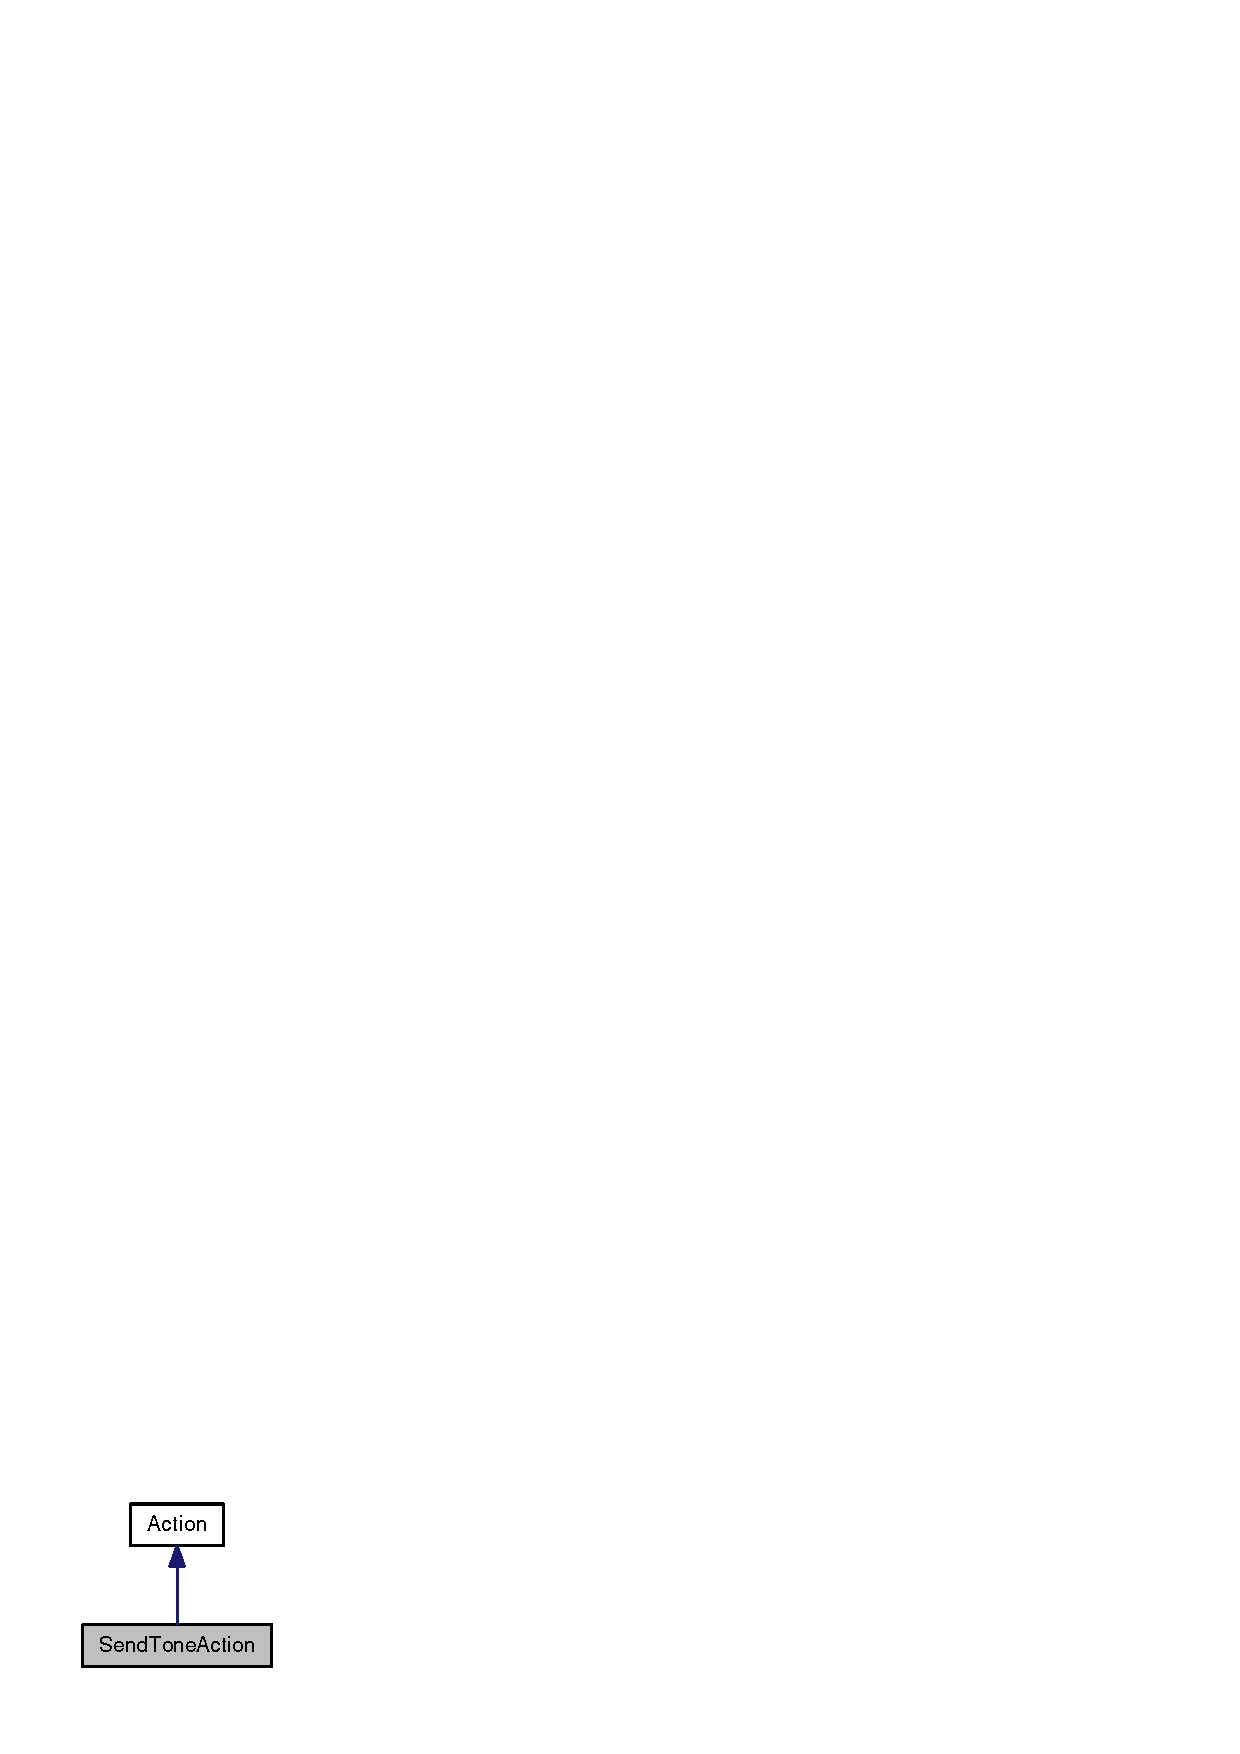
\includegraphics[width=134pt]{classSendToneAction__inherit__graph}
\end{center}
\end{figure}
Collaboration diagram for SendToneAction:\nopagebreak
\begin{figure}[H]
\begin{center}
\leavevmode
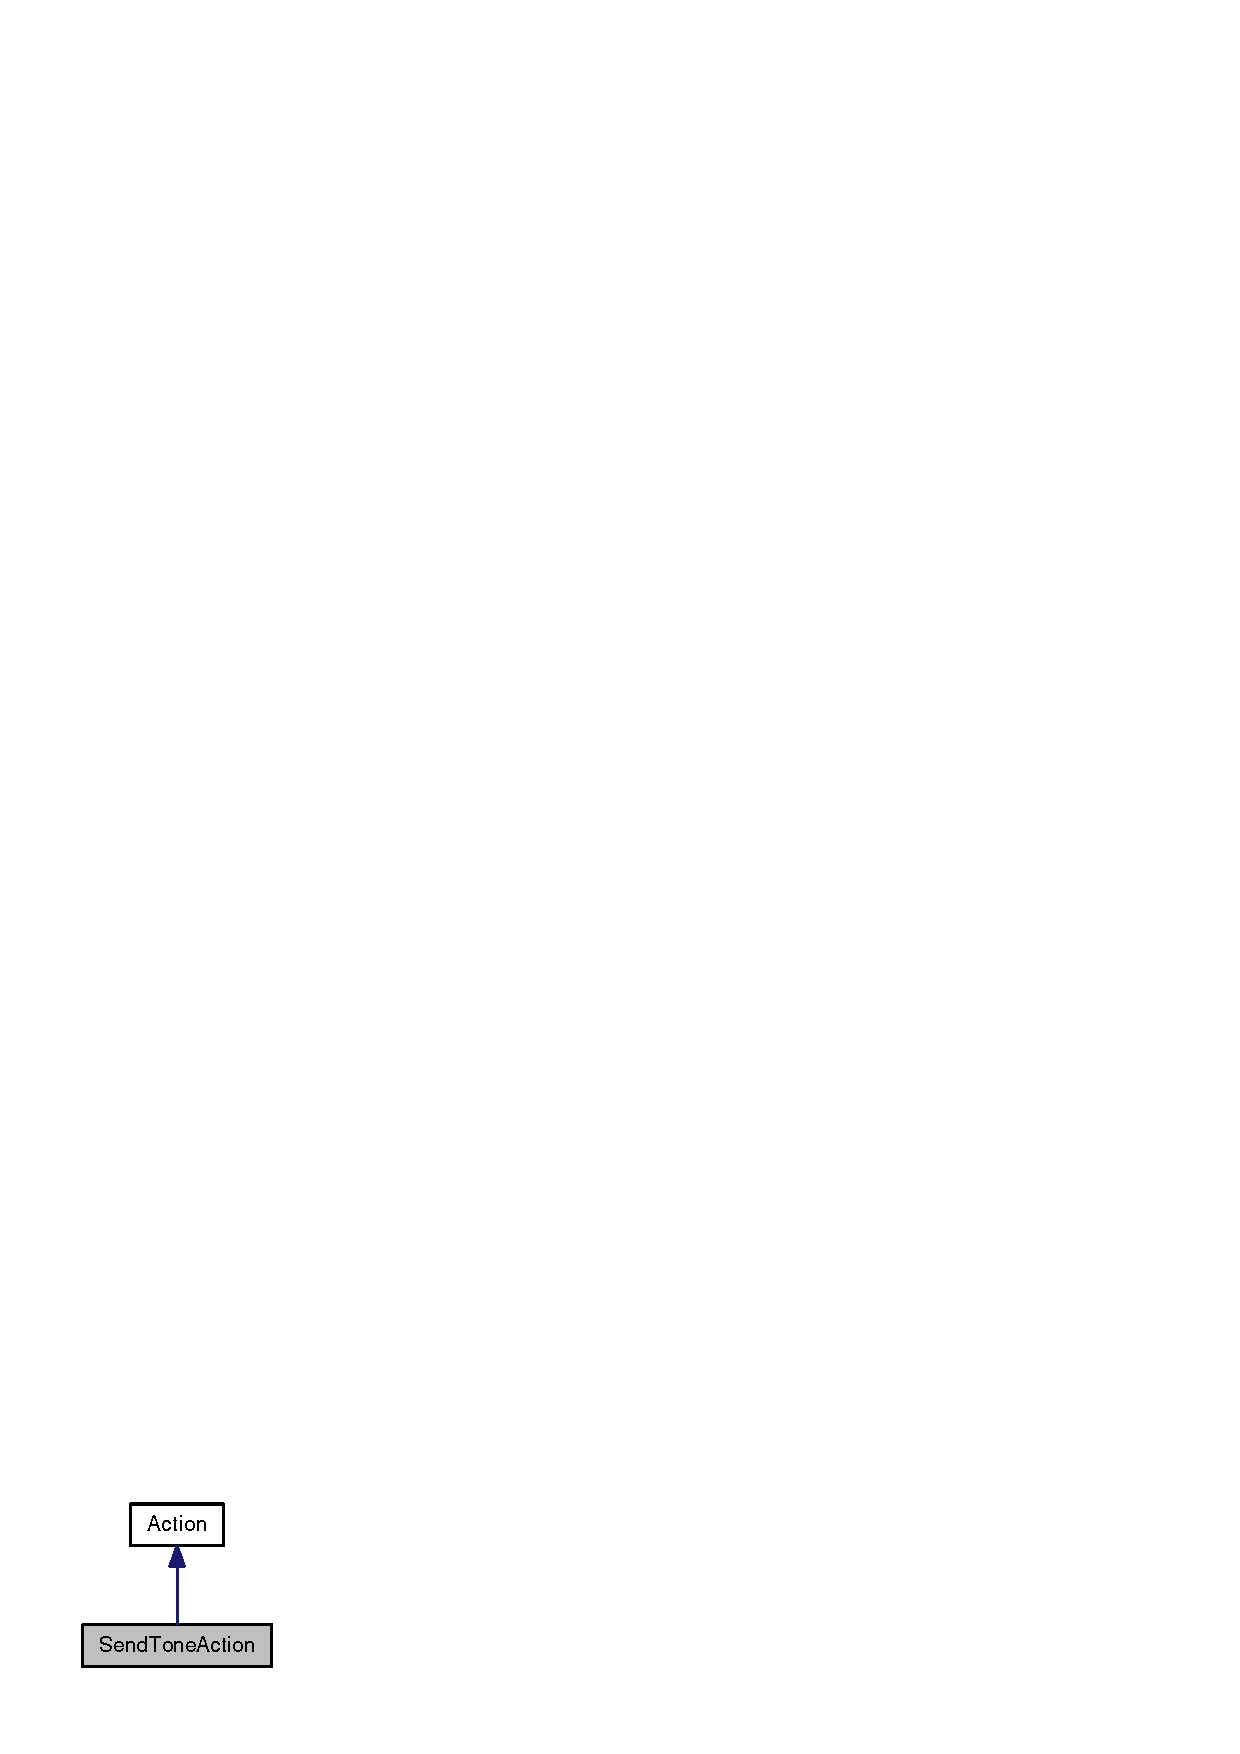
\includegraphics[width=134pt]{classSendToneAction__coll__graph}
\end{center}
\end{figure}
\subsection*{Public Member Functions}
\begin{CompactItemize}
\item 
\hyperlink{classSendToneAction_462b5171c72469683ab2d94e678cb955}{SendToneAction} (int \hyperlink{classAction_51e5d56a6aa4a037e90df19587a225c7}{turn}, char \hyperlink{classSendToneAction_971b5f50b925ee5e3ace27c909c0c3f9}{tone})
\end{CompactItemize}
\subsection*{Public Attributes}
\begin{CompactItemize}
\item 
const char \hyperlink{classSendToneAction_971b5f50b925ee5e3ace27c909c0c3f9}{tone}
\end{CompactItemize}


\subsection{Constructor \& Destructor Documentation}
\hypertarget{classSendToneAction_462b5171c72469683ab2d94e678cb955}{
\index{SendToneAction@{SendToneAction}!SendToneAction@{SendToneAction}}
\index{SendToneAction@{SendToneAction}!SendToneAction@{SendToneAction}}
\subsubsection[{SendToneAction}]{\setlength{\rightskip}{0pt plus 5cm}SendToneAction::SendToneAction (int {\em turn}, \/  char {\em tone})\hspace{0.3cm}{\tt  \mbox{[}inline\mbox{]}}}}
\label{classSendToneAction_462b5171c72469683ab2d94e678cb955}




\subsection{Member Data Documentation}
\hypertarget{classSendToneAction_971b5f50b925ee5e3ace27c909c0c3f9}{
\index{SendToneAction@{SendToneAction}!tone@{tone}}
\index{tone@{tone}!SendToneAction@{SendToneAction}}
\subsubsection[{tone}]{\setlength{\rightskip}{0pt plus 5cm}const char {\bf SendToneAction::tone}}}
\label{classSendToneAction_971b5f50b925ee5e3ace27c909c0c3f9}




The documentation for this class was generated from the following file:\begin{CompactItemize}
\item 
\hyperlink{action_8h}{action.h}\end{CompactItemize}

\hypertarget{classState}{
\section{State Class Reference}
\label{classState}\index{State@{State}}
}
{\tt \#include $<$state-new.h$>$}

\subsection*{Public Member Functions}
\begin{CompactItemize}
\item 
\hyperlink{classState_1b4e314c21378ef15c4ef854d4c88001}{State} (const int \hyperlink{classState_f747db9527dfb6ea0a58fe7bfeb3ac80}{id}, const int \hyperlink{classState_97418aee9e2f52608a6ab606c4594aff}{turn})
\item 
\hyperlink{classState_efadc9ab55d44f059e139b65c759dc14}{State} (\hyperlink{state_8h_2c309f64131cbfdae6d95e6591f208e6}{StateID} \hyperlink{classState_f747db9527dfb6ea0a58fe7bfeb3ac80}{id}, int \hyperlink{classState_97418aee9e2f52608a6ab606c4594aff}{turn})
\begin{CompactList}\small\item\em Constructor. \item\end{CompactList}\item 
\hyperlink{classState_0bfcbd427c3d009f71c627516ec17b25}{State} (\hyperlink{state_8h_2c309f64131cbfdae6d95e6591f208e6}{StateID} \hyperlink{classState_f747db9527dfb6ea0a58fe7bfeb3ac80}{id}, int \hyperlink{classState_97418aee9e2f52608a6ab606c4594aff}{turn}, \hyperlink{state_8h_26688ca6a181d6c6cf4f21d9839d4125}{StatusID} \hyperlink{classState_75d3a38b16f7081c4e961f6e7e2708b7}{status})
\begin{CompactList}\small\item\em Constructor. \item\end{CompactList}\item 
\hyperlink{classState_4ff7773f710d19259128cd975945b8d2}{State} (\hyperlink{state_8h_2c309f64131cbfdae6d95e6591f208e6}{StateID} \hyperlink{classState_f747db9527dfb6ea0a58fe7bfeb3ac80}{id}, int \hyperlink{classState_97418aee9e2f52608a6ab606c4594aff}{turn}, \hyperlink{state_8h_26688ca6a181d6c6cf4f21d9839d4125}{StatusID} \hyperlink{classState_75d3a38b16f7081c4e961f6e7e2708b7}{status}, const char $\ast$msg)
\begin{CompactList}\small\item\em Constructor. \item\end{CompactList}\item 
\hyperlink{classState_380fc79d928e017522e3b1c91e9aa66e}{State} (\hyperlink{state_8h_2c309f64131cbfdae6d95e6591f208e6}{StateID} \hyperlink{classState_f747db9527dfb6ea0a58fe7bfeb3ac80}{id}, int \hyperlink{classState_97418aee9e2f52608a6ab606c4594aff}{turn}, \hyperlink{state_8h_26688ca6a181d6c6cf4f21d9839d4125}{StatusID} \hyperlink{classState_75d3a38b16f7081c4e961f6e7e2708b7}{status}, const PString \&msg)
\begin{CompactList}\small\item\em Constructor. \item\end{CompactList}\item 
virtual \hyperlink{classState}{State} $\ast$ \hyperlink{classState_1e0489c0ec718afbb95d43edfcdafaab}{Clone} () const 
\begin{CompactList}\small\item\em Creates a copy of this class. \item\end{CompactList}\end{CompactItemize}
\subsection*{Public Attributes}
\begin{CompactItemize}
\item 
const int \hyperlink{classState_97418aee9e2f52608a6ab606c4594aff}{turn}
\begin{CompactList}\small\item\em Serial identifier used to conditionally accept action requests based on the state in which they were generated. \item\end{CompactList}\item 
const int \hyperlink{classState_f747db9527dfb6ea0a58fe7bfeb3ac80}{id}
\item 
const \hyperlink{state_8h_2c309f64131cbfdae6d95e6591f208e6}{StateID} \hyperlink{classState_3e78ec8b6887cfe32f68049e85398a42}{id}
\begin{CompactList}\small\item\em Uniquely identifies the state type. \item\end{CompactList}\item 
const \hyperlink{state_8h_26688ca6a181d6c6cf4f21d9839d4125}{StatusID} \hyperlink{classState_75d3a38b16f7081c4e961f6e7e2708b7}{status}
\begin{CompactList}\small\item\em Identifies the status associated with this state. \item\end{CompactList}\item 
const PString \hyperlink{classState_e85e97971c5a76295158e8225e468c32}{message}
\begin{CompactList}\small\item\em Empty string or a message that may be useful to display to the user relating to the status. \item\end{CompactList}\end{CompactItemize}


\subsection{Constructor \& Destructor Documentation}
\hypertarget{classState_1b4e314c21378ef15c4ef854d4c88001}{
\index{State@{State}!State@{State}}
\index{State@{State}!State@{State}}
\subsubsection[{State}]{\setlength{\rightskip}{0pt plus 5cm}State::State (const int {\em id}, \/  const int {\em turn})}}
\label{classState_1b4e314c21378ef15c4ef854d4c88001}


\hypertarget{classState_efadc9ab55d44f059e139b65c759dc14}{
\index{State@{State}!State@{State}}
\index{State@{State}!State@{State}}
\subsubsection[{State}]{\setlength{\rightskip}{0pt plus 5cm}State::State ({\bf StateID} {\em id}, \/  int {\em turn})}}
\label{classState_efadc9ab55d44f059e139b65c759dc14}


Constructor. 

\begin{Desc}
\item[Parameters:]
\begin{description}
\item[{\em id}]the type of this state \item[{\em turn}]previous state's id + 1 if previous state not of same type as this state; otherwise, previous state's turn \end{description}
\end{Desc}
\hypertarget{classState_0bfcbd427c3d009f71c627516ec17b25}{
\index{State@{State}!State@{State}}
\index{State@{State}!State@{State}}
\subsubsection[{State}]{\setlength{\rightskip}{0pt plus 5cm}State::State ({\bf StateID} {\em id}, \/  int {\em turn}, \/  {\bf StatusID} {\em status})}}
\label{classState_0bfcbd427c3d009f71c627516ec17b25}


Constructor. 

\begin{Desc}
\item[Parameters:]
\begin{description}
\item[{\em id}]the type of this state \item[{\em turn}]previous state's id + 1 if previous state not of same type as this state; otherwise, previous state's turn \item[{\em status}]the status to associate with this state \end{description}
\end{Desc}
\hypertarget{classState_4ff7773f710d19259128cd975945b8d2}{
\index{State@{State}!State@{State}}
\index{State@{State}!State@{State}}
\subsubsection[{State}]{\setlength{\rightskip}{0pt plus 5cm}State::State ({\bf StateID} {\em id}, \/  int {\em turn}, \/  {\bf StatusID} {\em status}, \/  const char $\ast$ {\em msg})}}
\label{classState_4ff7773f710d19259128cd975945b8d2}


Constructor. 

\begin{Desc}
\item[Parameters:]
\begin{description}
\item[{\em id}]the type of this state \item[{\em turn}]previous state's id + 1 if previous state not of same type as this state; otherwise, previous state's turn \item[{\em status}]the status to associate with this state \item[{\em msg}]user-friendly elaboration on the status \end{description}
\end{Desc}
\hypertarget{classState_380fc79d928e017522e3b1c91e9aa66e}{
\index{State@{State}!State@{State}}
\index{State@{State}!State@{State}}
\subsubsection[{State}]{\setlength{\rightskip}{0pt plus 5cm}State::State ({\bf StateID} {\em id}, \/  int {\em turn}, \/  {\bf StatusID} {\em status}, \/  const PString \& {\em msg})}}
\label{classState_380fc79d928e017522e3b1c91e9aa66e}


Constructor. 

\begin{Desc}
\item[Parameters:]
\begin{description}
\item[{\em id}]the type of this state \item[{\em turn}]previous state's id + 1 if previous state not of same type as this state; otherwise, previous state's turn \item[{\em status}]the status to associate with this state \item[{\em msg}]user-friendly elaboration on the status \end{description}
\end{Desc}


\subsection{Member Function Documentation}
\hypertarget{classState_1e0489c0ec718afbb95d43edfcdafaab}{
\index{State@{State}!Clone@{Clone}}
\index{Clone@{Clone}!State@{State}}
\subsubsection[{Clone}]{\setlength{\rightskip}{0pt plus 5cm}{\bf State} $\ast$ State::Clone () const\hspace{0.3cm}{\tt  \mbox{[}virtual\mbox{]}}}}
\label{classState_1e0489c0ec718afbb95d43edfcdafaab}


Creates a copy of this class. 

Subclasses must implement this method. 

\subsection{Member Data Documentation}
\hypertarget{classState_3e78ec8b6887cfe32f68049e85398a42}{
\index{State@{State}!id@{id}}
\index{id@{id}!State@{State}}
\subsubsection[{id}]{\setlength{\rightskip}{0pt plus 5cm}const {\bf StateID} {\bf State::id}}}
\label{classState_3e78ec8b6887cfe32f68049e85398a42}


Uniquely identifies the state type. 

\hypertarget{classState_f747db9527dfb6ea0a58fe7bfeb3ac80}{
\index{State@{State}!id@{id}}
\index{id@{id}!State@{State}}
\subsubsection[{id}]{\setlength{\rightskip}{0pt plus 5cm}const int {\bf State::id}}}
\label{classState_f747db9527dfb6ea0a58fe7bfeb3ac80}


\hypertarget{classState_e85e97971c5a76295158e8225e468c32}{
\index{State@{State}!message@{message}}
\index{message@{message}!State@{State}}
\subsubsection[{message}]{\setlength{\rightskip}{0pt plus 5cm}const PString {\bf State::message}}}
\label{classState_e85e97971c5a76295158e8225e468c32}


Empty string or a message that may be useful to display to the user relating to the status. 

\hypertarget{classState_75d3a38b16f7081c4e961f6e7e2708b7}{
\index{State@{State}!status@{status}}
\index{status@{status}!State@{State}}
\subsubsection[{status}]{\setlength{\rightskip}{0pt plus 5cm}const {\bf StatusID} {\bf State::status}}}
\label{classState_75d3a38b16f7081c4e961f6e7e2708b7}


Identifies the status associated with this state. 

\hypertarget{classState_97418aee9e2f52608a6ab606c4594aff}{
\index{State@{State}!turn@{turn}}
\index{turn@{turn}!State@{State}}
\subsubsection[{turn}]{\setlength{\rightskip}{0pt plus 5cm}const int {\bf State::turn}}}
\label{classState_97418aee9e2f52608a6ab606c4594aff}


Serial identifier used to conditionally accept action requests based on the state in which they were generated. 



The documentation for this class was generated from the following files:\begin{CompactItemize}
\item 
\hyperlink{state-new_8h}{state-new.h}\item 
\hyperlink{state_8h}{state.h}\item 
\hyperlink{state_8cpp}{state.cpp}\end{CompactItemize}

\hypertarget{classStateHelper}{
\section{StateHelper Class Reference}
\label{classStateHelper}\index{StateHelper@{StateHelper}}
}
Utilities for mapping state id and other state-derived data to meaningful semantics and messages.  


{\tt \#include $<$gui.h$>$}

\subsection*{Static Public Member Functions}
\begin{CompactItemize}
\item 
static wxString \hyperlink{classStateHelper_b33007a2d3887bbaff4acce948301579}{ToStatus} (const \hyperlink{state_8h_2c309f64131cbfdae6d95e6591f208e6}{StateID} \&state)
\begin{CompactList}\small\item\em Translate from state id to status bar message. \item\end{CompactList}\item 
static wxString \hyperlink{classStateHelper_c1c01103481e034cdcd4c679cf3bb45e}{ToTrace} (const \hyperlink{state_8h_2c309f64131cbfdae6d95e6591f208e6}{StateID} \&state, const \hyperlink{state_8h_26688ca6a181d6c6cf4f21d9839d4125}{StatusID} \&status, const wxString \&message, \hyperlink{classModel}{Model} $\ast$model, bool initialized)
\begin{CompactList}\small\item\em Generate a message suitable for display in the trace window. \item\end{CompactList}\item 
static bool \hyperlink{classStateHelper_2b3caf1bdd542b47e46dfbfedccead7f}{CanRegister} (const \hyperlink{state_8h_2c309f64131cbfdae6d95e6591f208e6}{StateID} \&state)
\begin{CompactList}\small\item\em Determine whether the registration is allowed. \item\end{CompactList}\item 
static bool \hyperlink{classStateHelper_dd3c36b37666dde08e682f49d999b510}{CanDial} (const \hyperlink{state_8h_2c309f64131cbfdae6d95e6591f208e6}{StateID} \&state)
\begin{CompactList}\small\item\em Determine whether a call can be placed in the current state. \item\end{CompactList}\item 
static bool \hyperlink{classStateHelper_c946e6f713969a2092d3e2c7ec004a7a}{CanHold} (const \hyperlink{state_8h_2c309f64131cbfdae6d95e6591f208e6}{StateID} \&state)
\begin{CompactList}\small\item\em Determine whether a connection exists and can be put on hold. \item\end{CompactList}\item 
static bool \hyperlink{classStateHelper_8ab96f1d7b7413154e5297ef22af93bb}{CanHangUp} (const \hyperlink{state_8h_2c309f64131cbfdae6d95e6591f208e6}{StateID} \&state)
\begin{CompactList}\small\item\em Determine whether hanging up is allowed. \item\end{CompactList}\item 
static bool \hyperlink{classStateHelper_a563c5e68e7da3e9b763d402da50605c}{CanRetrieve} (const \hyperlink{state_8h_2c309f64131cbfdae6d95e6591f208e6}{StateID} \&state)
\begin{CompactList}\small\item\em Determine whether it is possible to retrieve a call from any form of hold. \item\end{CompactList}\item 
static bool \hyperlink{classStateHelper_9c0a814cd8b3104a30dc9b6d5a4c1aab}{IsRegistered} (const \hyperlink{state_8h_2c309f64131cbfdae6d95e6591f208e6}{StateID} \&state)
\begin{CompactList}\small\item\em Determine whether the user is registered with a SIP registrar. \item\end{CompactList}\end{CompactItemize}


\subsection{Detailed Description}
Utilities for mapping state id and other state-derived data to meaningful semantics and messages. 

\subsection{Member Function Documentation}
\hypertarget{classStateHelper_dd3c36b37666dde08e682f49d999b510}{
\index{StateHelper@{StateHelper}!CanDial@{CanDial}}
\index{CanDial@{CanDial}!StateHelper@{StateHelper}}
\subsubsection[{CanDial}]{\setlength{\rightskip}{0pt plus 5cm}bool StateHelper::CanDial (const {\bf StateID} \& {\em state})\hspace{0.3cm}{\tt  \mbox{[}static\mbox{]}}}}
\label{classStateHelper_dd3c36b37666dde08e682f49d999b510}


Determine whether a call can be placed in the current state. 

Calls can be placed only in \hyperlink{}{STATE\_\-REGISTERED} state. \begin{Desc}
\item[Parameters:]
\begin{description}
\item[{\em state}]from \hyperlink{classState_f747db9527dfb6ea0a58fe7bfeb3ac80}{State\#id}. \end{description}
\end{Desc}
\hypertarget{classStateHelper_8ab96f1d7b7413154e5297ef22af93bb}{
\index{StateHelper@{StateHelper}!CanHangUp@{CanHangUp}}
\index{CanHangUp@{CanHangUp}!StateHelper@{StateHelper}}
\subsubsection[{CanHangUp}]{\setlength{\rightskip}{0pt plus 5cm}bool StateHelper::CanHangUp (const {\bf StateID} \& {\em state})\hspace{0.3cm}{\tt  \mbox{[}static\mbox{]}}}}
\label{classStateHelper_8ab96f1d7b7413154e5297ef22af93bb}


Determine whether hanging up is allowed. 

Hanging up is allowed at any time during dialing and any form of connected state, including hold and autohold, but not during the disconnection process or if it is known that the remote party has disconnected. \begin{Desc}
\item[Parameters:]
\begin{description}
\item[{\em state}]from \hyperlink{classState_f747db9527dfb6ea0a58fe7bfeb3ac80}{State\#id}. \end{description}
\end{Desc}
\hypertarget{classStateHelper_c946e6f713969a2092d3e2c7ec004a7a}{
\index{StateHelper@{StateHelper}!CanHold@{CanHold}}
\index{CanHold@{CanHold}!StateHelper@{StateHelper}}
\subsubsection[{CanHold}]{\setlength{\rightskip}{0pt plus 5cm}bool StateHelper::CanHold (const {\bf StateID} \& {\em state})\hspace{0.3cm}{\tt  \mbox{[}static\mbox{]}}}}
\label{classStateHelper_c946e6f713969a2092d3e2c7ec004a7a}


Determine whether a connection exists and can be put on hold. 

A call already on hold or autohold or not connected cannot be put on hold. \begin{Desc}
\item[Parameters:]
\begin{description}
\item[{\em state}]from \hyperlink{classState_f747db9527dfb6ea0a58fe7bfeb3ac80}{State\#id}. \end{description}
\end{Desc}
\hypertarget{classStateHelper_2b3caf1bdd542b47e46dfbfedccead7f}{
\index{StateHelper@{StateHelper}!CanRegister@{CanRegister}}
\index{CanRegister@{CanRegister}!StateHelper@{StateHelper}}
\subsubsection[{CanRegister}]{\setlength{\rightskip}{0pt plus 5cm}bool StateHelper::CanRegister (const {\bf StateID} \& {\em state})\hspace{0.3cm}{\tt  \mbox{[}static\mbox{]}}}}
\label{classStateHelper_2b3caf1bdd542b47e46dfbfedccead7f}


Determine whether the registration is allowed. 

\begin{Desc}
\item[Parameters:]
\begin{description}
\item[{\em state}]from \hyperlink{classState_f747db9527dfb6ea0a58fe7bfeb3ac80}{State\#id}. \end{description}
\end{Desc}
\hypertarget{classStateHelper_a563c5e68e7da3e9b763d402da50605c}{
\index{StateHelper@{StateHelper}!CanRetrieve@{CanRetrieve}}
\index{CanRetrieve@{CanRetrieve}!StateHelper@{StateHelper}}
\subsubsection[{CanRetrieve}]{\setlength{\rightskip}{0pt plus 5cm}bool StateHelper::CanRetrieve (const {\bf StateID} \& {\em state})\hspace{0.3cm}{\tt  \mbox{[}static\mbox{]}}}}
\label{classStateHelper_a563c5e68e7da3e9b763d402da50605c}


Determine whether it is possible to retrieve a call from any form of hold. 

A call must be on hold or autohold to be retrievable. \begin{Desc}
\item[Parameters:]
\begin{description}
\item[{\em state}]from \hyperlink{classState_f747db9527dfb6ea0a58fe7bfeb3ac80}{State\#id}. \end{description}
\end{Desc}
\hypertarget{classStateHelper_9c0a814cd8b3104a30dc9b6d5a4c1aab}{
\index{StateHelper@{StateHelper}!IsRegistered@{IsRegistered}}
\index{IsRegistered@{IsRegistered}!StateHelper@{StateHelper}}
\subsubsection[{IsRegistered}]{\setlength{\rightskip}{0pt plus 5cm}bool StateHelper::IsRegistered (const {\bf StateID} \& {\em state})\hspace{0.3cm}{\tt  \mbox{[}static\mbox{]}}}}
\label{classStateHelper_9c0a814cd8b3104a30dc9b6d5a4c1aab}


Determine whether the user is registered with a SIP registrar. 

\begin{Desc}
\item[Parameters:]
\begin{description}
\item[{\em state}]from \hyperlink{classState_f747db9527dfb6ea0a58fe7bfeb3ac80}{State\#id}. \end{description}
\end{Desc}
\hypertarget{classStateHelper_b33007a2d3887bbaff4acce948301579}{
\index{StateHelper@{StateHelper}!ToStatus@{ToStatus}}
\index{ToStatus@{ToStatus}!StateHelper@{StateHelper}}
\subsubsection[{ToStatus}]{\setlength{\rightskip}{0pt plus 5cm}wxString StateHelper::ToStatus (const {\bf StateID} \& {\em state})\hspace{0.3cm}{\tt  \mbox{[}static\mbox{]}}}}
\label{classStateHelper_b33007a2d3887bbaff4acce948301579}


Translate from state id to status bar message. 

\begin{Desc}
\item[Parameters:]
\begin{description}
\item[{\em state}]from \hyperlink{classState_f747db9527dfb6ea0a58fe7bfeb3ac80}{State\#id}. \end{description}
\end{Desc}
\hypertarget{classStateHelper_c1c01103481e034cdcd4c679cf3bb45e}{
\index{StateHelper@{StateHelper}!ToTrace@{ToTrace}}
\index{ToTrace@{ToTrace}!StateHelper@{StateHelper}}
\subsubsection[{ToTrace}]{\setlength{\rightskip}{0pt plus 5cm}wxString StateHelper::ToTrace (const {\bf StateID} \& {\em state}, \/  const {\bf StatusID} \& {\em status}, \/  const wxString \& {\em message}, \/  {\bf Model} $\ast$ {\em model}, \/  bool {\em initialized})\hspace{0.3cm}{\tt  \mbox{[}static\mbox{]}}}}
\label{classStateHelper_c1c01103481e034cdcd4c679cf3bb45e}


Generate a message suitable for display in the trace window. 

\begin{Desc}
\item[Parameters:]
\begin{description}
\item[{\em state}]from \hyperlink{classState_f747db9527dfb6ea0a58fe7bfeb3ac80}{State\#id}. \item[{\em status}]from \hyperlink{classState_f747db9527dfb6ea0a58fe7bfeb3ac80}{State\#id}. \item[{\em message}]from \hyperlink{classState_f747db9527dfb6ea0a58fe7bfeb3ac80}{State\#id}., converted to wxString. \item[{\em model}]the \hyperlink{classModel}{Model}. \item[{\em initialized}]true if \hyperlink{state_8h_2c309f64131cbfdae6d95e6591f208e6033f1b9c62140635eb6f0e3035a72c34}{State\#STATE\_\-INITIALIZED} has already been seen at least once. \end{description}
\end{Desc}


The documentation for this class was generated from the following files:\begin{CompactItemize}
\item 
\hyperlink{gui_8h}{gui.h}\item 
\hyperlink{gui_8cpp}{gui.cpp}\end{CompactItemize}

\hypertarget{classTeleKarma}{
\section{TeleKarma Class Reference}
\label{classTeleKarma}\index{TeleKarma@{TeleKarma}}
}
{\tt \#include $<$telekarma.h$>$}

Inheritance diagram for TeleKarma:\nopagebreak
\begin{figure}[H]
\begin{center}
\leavevmode

\includegraphics[width=110pt]{classTeleKarma__inherit__graph}
\end{center}
\end{figure}
Collaboration diagram for TeleKarma:\nopagebreak
\begin{figure}[H]
\begin{center}
\leavevmode

\includegraphics[width=298pt]{classTeleKarma__coll__graph}
\end{center}
\end{figure}
\subsection*{Public Member Functions}
\begin{CompactItemize}
\item 
\hyperlink{classTeleKarma_ffedc7e09446314b687922735cd7818f}{TeleKarma} (\hyperlink{classModel}{Model} $\ast$\hyperlink{classController_6f6ea54052742d3940adfcfce885bae9}{model})
\begin{CompactList}\small\item\em Constructor. \item\end{CompactList}\item 
void \hyperlink{classTeleKarma_addd554bf6335422cc896c894005a031}{Main} ()
\end{CompactItemize}


\subsection{Detailed Description}
The \hyperlink{classTeleKarma}{TeleKarma} class provides the \char`\"{}main\char`\"{} function for the \hyperlink{classTeleKarma}{TeleKarma} application and provides the interface through which state handler objects access information and take action. 

The Main function, which is invoked by PTLib tools from \hyperlink{main_8cpp}{main.cpp}, sets up state handler objects, sets the initial state, and enters a loop that invokes the \hyperlink{}{StateHandler\#In()} method and sleeps for \hyperlink{telekarma_8h_4af2a8a383f07fec0d9f78f2db1c987a}{SLEEP\_\-DURATION} milliseconds. 

All other methods support state handler methods, which for the sake of modularity have access to this class, but are not provided direct access to the telephony interface or other resources.  

\subsection{Constructor \& Destructor Documentation}
\hypertarget{classTeleKarma_ffedc7e09446314b687922735cd7818f}{
\index{TeleKarma@{TeleKarma}!TeleKarma@{TeleKarma}}
\index{TeleKarma@{TeleKarma}!TeleKarma@{TeleKarma}}
\subsubsection[{TeleKarma}]{\setlength{\rightskip}{0pt plus 5cm}TeleKarma::TeleKarma ({\bf Model} $\ast$ {\em model})}}
\label{classTeleKarma_ffedc7e09446314b687922735cd7818f}


Constructor. 

Initializes fields. \begin{Desc}
\item[Parameters:]
\begin{description}
\item[{\em model}]\end{description}
\end{Desc}


\subsection{Member Function Documentation}
\hypertarget{classTeleKarma_addd554bf6335422cc896c894005a031}{
\index{TeleKarma@{TeleKarma}!Main@{Main}}
\index{Main@{Main}!TeleKarma@{TeleKarma}}
\subsubsection[{Main}]{\setlength{\rightskip}{0pt plus 5cm}void TeleKarma::Main ()\hspace{0.3cm}{\tt  \mbox{[}virtual\mbox{]}}}}
\label{classTeleKarma_addd554bf6335422cc896c894005a031}


Main program logic. Verifies existance of required subfolders, sets up log files, instantiate state handler objects, sets the initial state handler and enters main control loop. 

Main control loop simply calls the \hyperlink{}{StateHandler\#In()} method, then sleeps, then repeats, until the state handler is set to an instance of \hyperlink{}{ExitStateHandler}. States call the \hyperlink{}{EnterState(int)} method to change TeleKarma's state.  

Implements \hyperlink{classController_efeb521047c5b5d1c3f97290d015cacf}{Controller}.

The documentation for this class was generated from the following files:\begin{CompactItemize}
\item 
\hyperlink{telekarma_8h}{telekarma.h}\item 
\hyperlink{telekarma_8cpp}{telekarma.cpp}\end{CompactItemize}

\hypertarget{classTeleKarmaNG}{
\section{TeleKarmaNG Class Reference}
\label{classTeleKarmaNG}\index{TeleKarmaNG@{TeleKarmaNG}}
}
The main process.  


{\tt \#include $<$gui.h$>$}

Inheritance diagram for TeleKarmaNG:\nopagebreak
\begin{figure}[H]
\begin{center}
\leavevmode

\includegraphics[width=126pt]{classTeleKarmaNG__inherit__graph}
\end{center}
\end{figure}
Collaboration diagram for TeleKarmaNG:\nopagebreak
\begin{figure}[H]
\begin{center}
\leavevmode

\includegraphics[height=400pt]{classTeleKarmaNG__coll__graph}
\end{center}
\end{figure}
\subsection*{Public Member Functions}
\begin{CompactItemize}
\item 
\hyperlink{classTeleKarmaNG_a0decf4d37075fe5a6ca8009996f9cce}{$\sim$TeleKarmaNG} ()
\begin{CompactList}\small\item\em Destructor waits for child threads. \item\end{CompactList}\item 
void \hyperlink{classTeleKarmaNG_9e2c67bec8a3794e755ee1d91a18a9fa}{Main} ()
\begin{CompactList}\small\item\em A dummy method for the benefit of PProcess. \item\end{CompactList}\item 
bool \hyperlink{classTeleKarmaNG_87ccb2d5650091ba595c4b7bd832d752}{OnInit} ()
\begin{CompactList}\small\item\em Fulfills wxApp requirement. \item\end{CompactList}\item 
void \hyperlink{classTeleKarmaNG_ce1e8d62f3e1d586e2aa5d2012c9a766}{OnStateChange} ()
\begin{CompactList}\small\item\em Callback for \hyperlink{classModel}{Model} upon state change (see \hyperlink{classModelListener}{ModelListener}). \item\end{CompactList}\item 
void \hyperlink{classTeleKarmaNG_54349ac49ff1575dfd1b158ef0842895}{OnCloseApplication} ()
\begin{CompactList}\small\item\em Callback for \hyperlink{classMainFrame}{MainFrame} upon termination. \item\end{CompactList}\item 
void \hyperlink{classTeleKarmaNG_cf965461b8261feb570acbaa88e4452d}{Quit} ()
\begin{CompactList}\small\item\em Exit handler. \item\end{CompactList}\end{CompactItemize}


\subsection{Detailed Description}
The main process. 

\subsection{Constructor \& Destructor Documentation}
\hypertarget{classTeleKarmaNG_a0decf4d37075fe5a6ca8009996f9cce}{
\index{TeleKarmaNG@{TeleKarmaNG}!$\sim$TeleKarmaNG@{$\sim$TeleKarmaNG}}
\index{$\sim$TeleKarmaNG@{$\sim$TeleKarmaNG}!TeleKarmaNG@{TeleKarmaNG}}
\subsubsection[{$\sim$TeleKarmaNG}]{\setlength{\rightskip}{0pt plus 5cm}TeleKarmaNG::$\sim$TeleKarmaNG ()}}
\label{classTeleKarmaNG_a0decf4d37075fe5a6ca8009996f9cce}


Destructor waits for child threads. 



\subsection{Member Function Documentation}
\hypertarget{classTeleKarmaNG_9e2c67bec8a3794e755ee1d91a18a9fa}{
\index{TeleKarmaNG@{TeleKarmaNG}!Main@{Main}}
\index{Main@{Main}!TeleKarmaNG@{TeleKarmaNG}}
\subsubsection[{Main}]{\setlength{\rightskip}{0pt plus 5cm}void TeleKarmaNG::Main ()\hspace{0.3cm}{\tt  \mbox{[}inline\mbox{]}}}}
\label{classTeleKarmaNG_9e2c67bec8a3794e755ee1d91a18a9fa}


A dummy method for the benefit of PProcess. 

\hypertarget{classTeleKarmaNG_54349ac49ff1575dfd1b158ef0842895}{
\index{TeleKarmaNG@{TeleKarmaNG}!OnCloseApplication@{OnCloseApplication}}
\index{OnCloseApplication@{OnCloseApplication}!TeleKarmaNG@{TeleKarmaNG}}
\subsubsection[{OnCloseApplication}]{\setlength{\rightskip}{0pt plus 5cm}void TeleKarmaNG::OnCloseApplication ()}}
\label{classTeleKarmaNG_54349ac49ff1575dfd1b158ef0842895}


Callback for \hyperlink{classMainFrame}{MainFrame} upon termination. 

\hypertarget{classTeleKarmaNG_87ccb2d5650091ba595c4b7bd832d752}{
\index{TeleKarmaNG@{TeleKarmaNG}!OnInit@{OnInit}}
\index{OnInit@{OnInit}!TeleKarmaNG@{TeleKarmaNG}}
\subsubsection[{OnInit}]{\setlength{\rightskip}{0pt plus 5cm}bool TeleKarmaNG::OnInit ()}}
\label{classTeleKarmaNG_87ccb2d5650091ba595c4b7bd832d752}


Fulfills wxApp requirement. 

\hypertarget{classTeleKarmaNG_ce1e8d62f3e1d586e2aa5d2012c9a766}{
\index{TeleKarmaNG@{TeleKarmaNG}!OnStateChange@{OnStateChange}}
\index{OnStateChange@{OnStateChange}!TeleKarmaNG@{TeleKarmaNG}}
\subsubsection[{OnStateChange}]{\setlength{\rightskip}{0pt plus 5cm}void TeleKarmaNG::OnStateChange ()\hspace{0.3cm}{\tt  \mbox{[}virtual\mbox{]}}}}
\label{classTeleKarmaNG_ce1e8d62f3e1d586e2aa5d2012c9a766}


Callback for \hyperlink{classModel}{Model} upon state change (see \hyperlink{classModelListener}{ModelListener}). 



Reimplemented from \hyperlink{classView_92a0d9fd64b52e7f85d45c46c28a6546}{View}.\hypertarget{classTeleKarmaNG_cf965461b8261feb570acbaa88e4452d}{
\index{TeleKarmaNG@{TeleKarmaNG}!Quit@{Quit}}
\index{Quit@{Quit}!TeleKarmaNG@{TeleKarmaNG}}
\subsubsection[{Quit}]{\setlength{\rightskip}{0pt plus 5cm}void TeleKarmaNG::Quit ()}}
\label{classTeleKarmaNG_cf965461b8261feb570acbaa88e4452d}


Exit handler. 



The documentation for this class was generated from the following files:\begin{CompactItemize}
\item 
\hyperlink{gui_8h}{gui.h}\item 
\hyperlink{gui_8cpp}{gui.cpp}\end{CompactItemize}

\hypertarget{classTelephonyIfc}{
\section{TelephonyIfc Class Reference}
\label{classTelephonyIfc}\index{TelephonyIfc@{TelephonyIfc}}
}
This class is the interface between telekarama and the Opal telephony library.  


{\tt \#include $<$telephony.h$>$}

Collaboration diagram for TelephonyIfc:\nopagebreak
\begin{figure}[H]
\begin{center}
\leavevmode
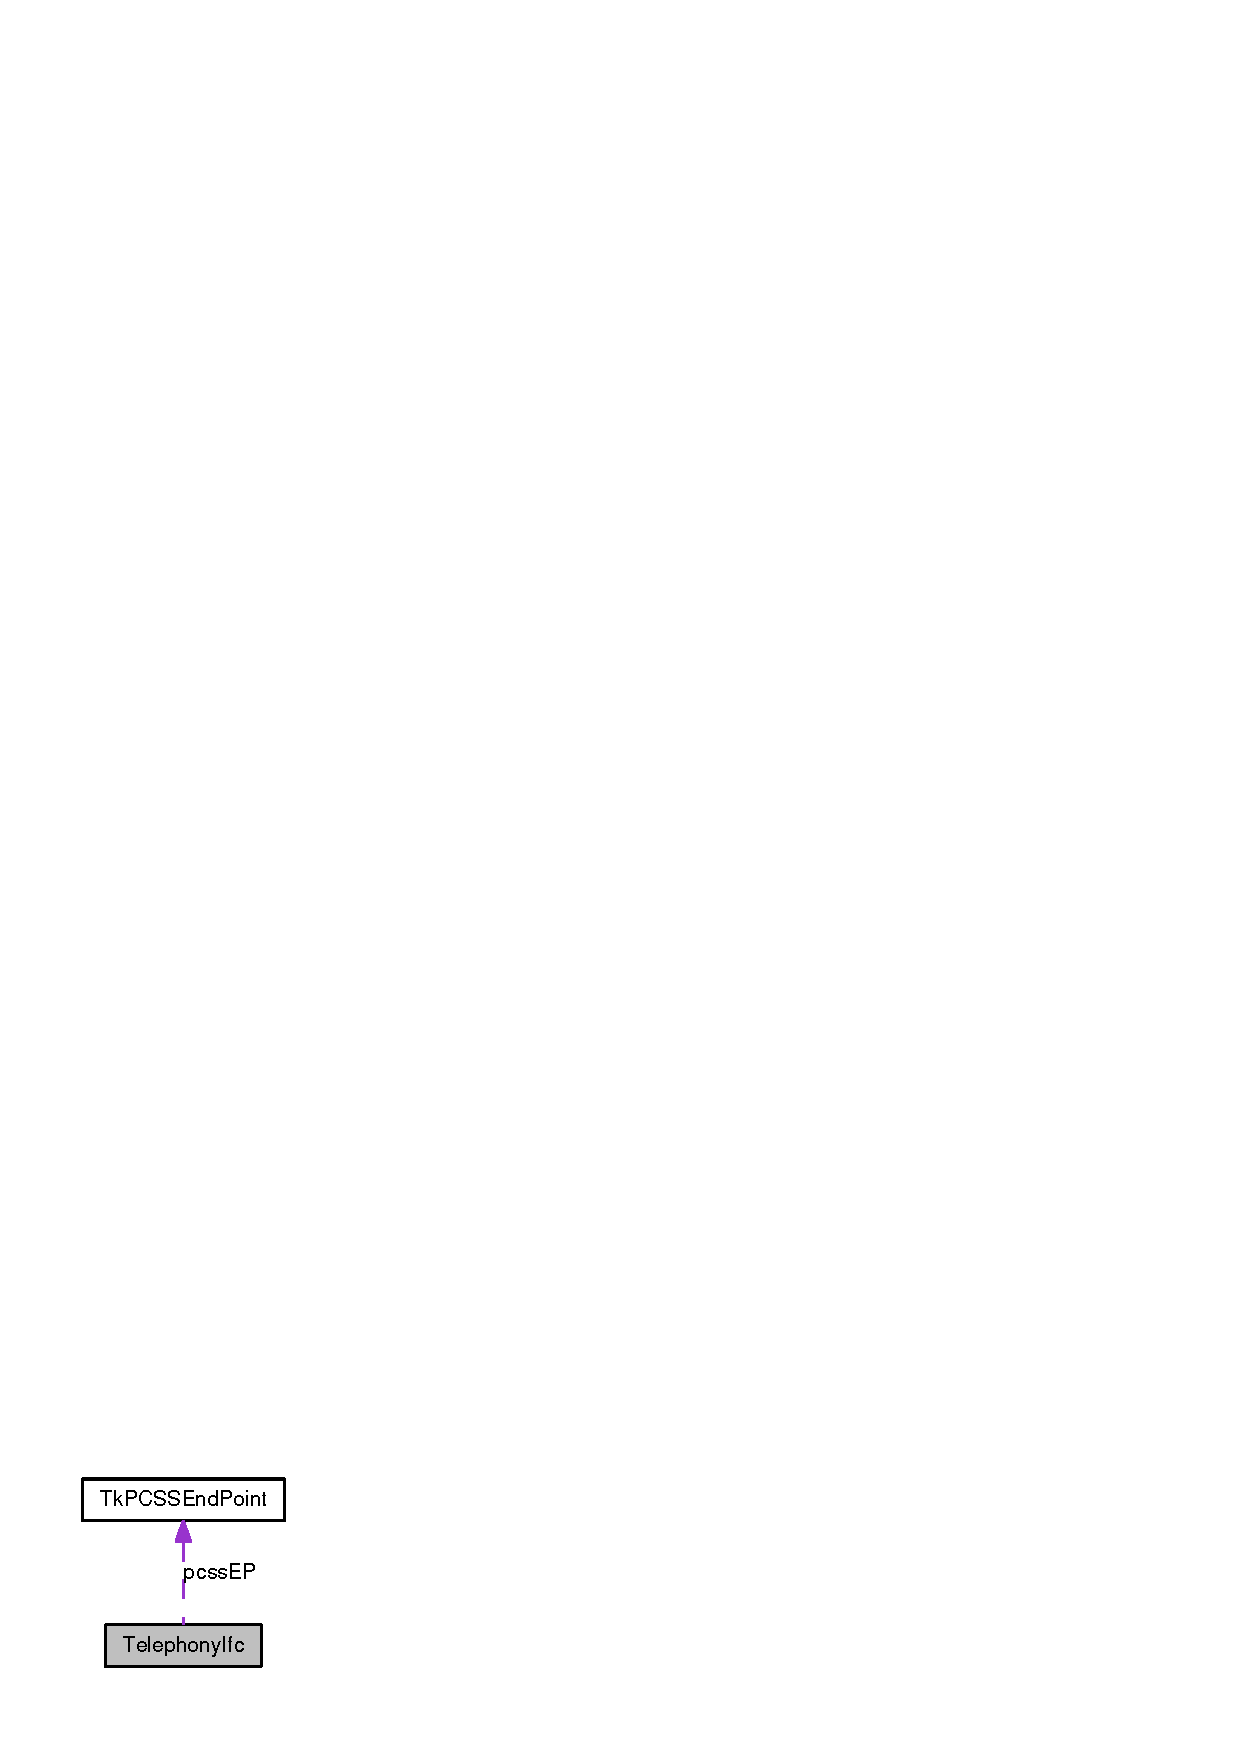
\includegraphics[height=400pt]{classTelephonyIfc__coll__graph}
\end{center}
\end{figure}
\subsection*{Public Member Functions}
\begin{CompactItemize}
\item 
void \hyperlink{classTelephonyIfc_f9e1672e2302bd86c082070db8cf9b9f}{Initialise} (const PString \&stunAddr, const PString \&user)
\begin{CompactList}\small\item\em Set up the \hyperlink{classTelephonyIfc}{TelephonyIfc} class. \item\end{CompactList}\item 
void \hyperlink{classTelephonyIfc_ddbfc63168d5e70fd4f83469de4aabb7}{Register} (const PString \&registrar, const PString \&user, const PString \&passwd)
\begin{CompactList}\small\item\em Register with a service provided. \item\end{CompactList}\item 
\hypertarget{classTelephonyIfc_20e9a9dd2df97b6c50aa1e19191c890a}{
PBoolean \hyperlink{classTelephonyIfc_20e9a9dd2df97b6c50aa1e19191c890a}{IsRegistered} ()}
\label{classTelephonyIfc_20e9a9dd2df97b6c50aa1e19191c890a}

\begin{CompactList}\small\item\em Indicates whether the user is registered with a SIP provider. \item\end{CompactList}\item 
\hypertarget{classTelephonyIfc_957da4a7936c3672a48f0fa93f655676}{
PBoolean \hyperlink{classTelephonyIfc_957da4a7936c3672a48f0fa93f655676}{Unregister} ()}
\label{classTelephonyIfc_957da4a7936c3672a48f0fa93f655676}

\begin{CompactList}\small\item\em Unregister from the current SIP provider. \item\end{CompactList}\item 
PBoolean \hyperlink{classTelephonyIfc_4acdd44e7af7967ed53cdf9d47dc0c27}{IsRecording} ()
\item 
void \hyperlink{classTelephonyIfc_2cd8176d99232038fbe8718417135b07}{StartRecording} (const PString \&fname)
\begin{CompactList}\small\item\em Begin recording the current call. \item\end{CompactList}\item 
\hypertarget{classTelephonyIfc_14352867be8fe5f0fcf501701e9052b2}{
void \hyperlink{classTelephonyIfc_14352867be8fe5f0fcf501701e9052b2}{StopRecording} ()}
\label{classTelephonyIfc_14352867be8fe5f0fcf501701e9052b2}

\begin{CompactList}\small\item\em Stop recording the current call. \item\end{CompactList}\item 
bool \hyperlink{classTelephonyIfc_60cba0b92e2f33357c063c251fae2997}{ToneReceived} (char key, bool clear=true)
\begin{CompactList}\small\item\em Determines whether a DTMF tone has been received. \item\end{CompactList}\item 
void \hyperlink{classTelephonyIfc_ac6179d75a2c623e05ccb345b45741f1}{SendTone} (const char tone)
\begin{CompactList}\small\item\em Send a DTMF tone to the remote party if connected. \item\end{CompactList}\item 
void \hyperlink{classTelephonyIfc_2e0adbafa63cd9c07a1c1c6ce68bf933}{Dial} (const PString \&ostr)
\begin{CompactList}\small\item\em Initiate a new call. \item\end{CompactList}\item 
\hypertarget{classTelephonyIfc_074e1d67c95ce1e66d346bb7315d5dcd}{
PBoolean \hyperlink{classTelephonyIfc_074e1d67c95ce1e66d346bb7315d5dcd}{IsDialing} ()}
\label{classTelephonyIfc_074e1d67c95ce1e66d346bb7315d5dcd}

\begin{CompactList}\small\item\em Determines whether there is a call being dialed, but not yet connected. \item\end{CompactList}\item 
void \hyperlink{classTelephonyIfc_a482ebd5daf3bf5d69ec40a46a0616e9}{OnEstablishedCall} (OpalCall \&call)
\begin{CompactList}\small\item\em Callback invoked when call has been established. \item\end{CompactList}\item 
\hypertarget{classTelephonyIfc_2a68749063e9e0c45ac31e8e44fa0849}{
PBoolean \hyperlink{classTelephonyIfc_2a68749063e9e0c45ac31e8e44fa0849}{IsConnected} ()}
\label{classTelephonyIfc_2a68749063e9e0c45ac31e8e44fa0849}

\begin{CompactList}\small\item\em Determines whether there is a connected call. \item\end{CompactList}\item 
void \hyperlink{classTelephonyIfc_68160576582be102ace0f4ae277d7129}{Disconnect} ()
\begin{CompactList}\small\item\em Disconnect the current call if it exists. \item\end{CompactList}\item 
void \hyperlink{classTelephonyIfc_7efa2a51fd26f3c5072ee8b7ba09d75c}{OnClearedCall} (OpalCall \&call)
\begin{CompactList}\small\item\em Callback invoked when call has been disconnected. \item\end{CompactList}\item 
\hypertarget{classTelephonyIfc_d5e6a50893f0915064f23c8d50de481f}{
PString \hyperlink{classTelephonyIfc_d5e6a50893f0915064f23c8d50de481f}{DisconnectReason} ()}
\label{classTelephonyIfc_d5e6a50893f0915064f23c8d50de481f}

\begin{CompactList}\small\item\em Returns a human-friendly description of the reason a call ended or NULL. \item\end{CompactList}\item 
PBoolean \hyperlink{classTelephonyIfc_f3a2ff3766cf45c203dba5a2260445b1}{OnOpenMediaStream} (OpalConnection \&connection, OpalMediaStream \&stream)
\begin{CompactList}\small\item\em Callback invoked when a media stream is opened for reading or playing. \item\end{CompactList}\item 
void \hyperlink{classTelephonyIfc_085ab0d59a990bda8b17cb56b1baaeb1}{OnUserInputTone} (OpalConnection \&connection, char tone, int duration)
\begin{CompactList}\small\item\em Callback invoked when DTMF tone is detected. \item\end{CompactList}\item 
\hypertarget{classTelephonyIfc_c471d58342002859cc9a59b1d1e494ca}{
void \hyperlink{classTelephonyIfc_c471d58342002859cc9a59b1d1e494ca}{ClearTones} ()}
\label{classTelephonyIfc_c471d58342002859cc9a59b1d1e494ca}

\begin{CompactList}\small\item\em Clears the array that holds a record of unique tones received since the last time the array was cleared. \item\end{CompactList}\item 
PBoolean \hyperlink{classTelephonyIfc_1138529389af3b4712bd11fadd4836ca}{PlayWAV} (const PString \&path, int repeat=0, int delay=0)
\begin{CompactList}\small\item\em Transmit a WAV file to the remote party. \item\end{CompactList}\item 
\hypertarget{classTelephonyIfc_6bf03dc65c5128fc1b7c299a6e40740f}{
void \hyperlink{classTelephonyIfc_6bf03dc65c5128fc1b7c299a6e40740f}{StopWAV} ()}
\label{classTelephonyIfc_6bf03dc65c5128fc1b7c299a6e40740f}

\begin{CompactList}\small\item\em Stop the WAV file that is currently playing. \item\end{CompactList}\item 
\hypertarget{classTelephonyIfc_a471fa455406339841ed30bddedb7dab}{
PBoolean \textbf{IsPlayingWav} ()}
\label{classTelephonyIfc_a471fa455406339841ed30bddedb7dab}

\item 
\hypertarget{classTelephonyIfc_e5318586774b3cae6afd9bd3596ac0a6}{
void \hyperlink{classTelephonyIfc_e5318586774b3cae6afd9bd3596ac0a6}{Retrieve} ()}
\label{classTelephonyIfc_e5318586774b3cae6afd9bd3596ac0a6}

\begin{CompactList}\small\item\em Retrieve the call from any form of IVR mode. \item\end{CompactList}\item 
\hypertarget{classTelephonyIfc_9c7068e7f0ef2d4498272b4a20361d4c}{
void \hyperlink{classTelephonyIfc_9c7068e7f0ef2d4498272b4a20361d4c}{SetMicVolume} (unsigned int gain)}
\label{classTelephonyIfc_9c7068e7f0ef2d4498272b4a20361d4c}

\begin{CompactList}\small\item\em Set the gain (volume) of the microphone. \item\end{CompactList}\item 
\hypertarget{classTelephonyIfc_8cf9b680409dfad0e8453a93b1057af2}{
void \hyperlink{classTelephonyIfc_8cf9b680409dfad0e8453a93b1057af2}{SetSpeakerVolume} (unsigned int gain)}
\label{classTelephonyIfc_8cf9b680409dfad0e8453a93b1057af2}

\begin{CompactList}\small\item\em Set the gain (volume) of the pc's speakers or other sound output device. \item\end{CompactList}\item 
\hypertarget{classTelephonyIfc_4b81a2cfb03620cd829e8da73dfe0ea4}{
void \hyperlink{classTelephonyIfc_4b81a2cfb03620cd829e8da73dfe0ea4}{TurnOffMicrophone} ()}
\label{classTelephonyIfc_4b81a2cfb03620cd829e8da73dfe0ea4}

\begin{CompactList}\small\item\em Block all microphone input. \item\end{CompactList}\item 
\hypertarget{classTelephonyIfc_d5ecca9d510408b2ce43cb5b5071b357}{
void \hyperlink{classTelephonyIfc_d5ecca9d510408b2ce43cb5b5071b357}{TurnOnMicrophone} ()}
\label{classTelephonyIfc_d5ecca9d510408b2ce43cb5b5071b357}

\begin{CompactList}\small\item\em Un-Block all microphone input. \item\end{CompactList}\end{CompactItemize}
\subsection*{Protected Member Functions}
\begin{CompactItemize}
\item 
\hypertarget{classTelephonyIfc_95f4177c87b299ab8dd0a2a13a319e0e}{
void \textbf{OnAudioFileSent} ()}
\label{classTelephonyIfc_95f4177c87b299ab8dd0a2a13a319e0e}

\end{CompactItemize}
\subsection*{Protected Attributes}
\begin{CompactItemize}
\item 
\hypertarget{classTelephonyIfc_3541fbc8e53e233226678ef3033b591f}{
PString \hyperlink{classTelephonyIfc_3541fbc8e53e233226678ef3033b591f}{callToken}}
\label{classTelephonyIfc_3541fbc8e53e233226678ef3033b591f}

\begin{CompactList}\small\item\em Call token for the connection from telekarama to the remote party. \item\end{CompactList}\item 
\hypertarget{classTelephonyIfc_86cd9e4c5ffe313c8aa4b73b02a02a47}{
PString \hyperlink{classTelephonyIfc_86cd9e4c5ffe313c8aa4b73b02a02a47}{pcToken}}
\label{classTelephonyIfc_86cd9e4c5ffe313c8aa4b73b02a02a47}

\begin{CompactList}\small\item\em Call token for the connection from telekarama to the PC sound system. \item\end{CompactList}\item 
\hypertarget{classTelephonyIfc_54799c28302aba6f7adb8c8ef438503e}{
PString \hyperlink{classTelephonyIfc_54799c28302aba6f7adb8c8ef438503e}{wavToken}}
\label{classTelephonyIfc_54799c28302aba6f7adb8c8ef438503e}

\begin{CompactList}\small\item\em Call token used to reference the WAV file that is currently playing. \item\end{CompactList}\item 
\hypertarget{classTelephonyIfc_616675027eef53f520b9ac96b81a56b0}{
PString \hyperlink{classTelephonyIfc_616675027eef53f520b9ac96b81a56b0}{recordToken}}
\label{classTelephonyIfc_616675027eef53f520b9ac96b81a56b0}

\begin{CompactList}\small\item\em Call token for the connection from telekarma to the recording device. \item\end{CompactList}\item 
\hypertarget{classTelephonyIfc_b4e274c6a138a5e08ead646eda38613e}{
PString \textbf{aor}}
\label{classTelephonyIfc_b4e274c6a138a5e08ead646eda38613e}

\item 
\hypertarget{classTelephonyIfc_0ffb35f802c55694b5729e5bde971483}{
bool \hyperlink{classTelephonyIfc_0ffb35f802c55694b5729e5bde971483}{dialing}}
\label{classTelephonyIfc_0ffb35f802c55694b5729e5bde971483}

\begin{CompactList}\small\item\em PTrue if telekarma is dialing a remote party otherwise PFalse. \item\end{CompactList}\item 
\hypertarget{classTelephonyIfc_377903745950f7376b919c2a4456debd}{
PBoolean \hyperlink{classTelephonyIfc_377903745950f7376b919c2a4456debd}{ivrMode}}
\label{classTelephonyIfc_377903745950f7376b919c2a4456debd}

\begin{CompactList}\small\item\em PTrue if telekarma is in IVR mode otherwise PFalse. \item\end{CompactList}\item 
\hypertarget{classTelephonyIfc_f41ebe765b20a522ebd9c493c3bf77eb}{
PString \hyperlink{classTelephonyIfc_f41ebe765b20a522ebd9c493c3bf77eb}{why}}
\label{classTelephonyIfc_f41ebe765b20a522ebd9c493c3bf77eb}

\begin{CompactList}\small\item\em Describes why call was disconnected. \item\end{CompactList}\item 
\hypertarget{classTelephonyIfc_8c18969f7ee88659b8b118c530f79bcd}{
char \hyperlink{classTelephonyIfc_8c18969f7ee88659b8b118c530f79bcd}{tones} \mbox{[}DTMF\_\-TONE\_\-MAX\mbox{]}}
\label{classTelephonyIfc_8c18969f7ee88659b8b118c530f79bcd}

\begin{CompactList}\small\item\em Queue of tones pressed by the remote user. \item\end{CompactList}\item 
\hypertarget{classTelephonyIfc_b857d1530a322453a8788c9bffbcc833}{
int \textbf{nextTone}}
\label{classTelephonyIfc_b857d1530a322453a8788c9bffbcc833}

\item 
\hypertarget{classTelephonyIfc_692107ad53586332c50b34ea3b51f76d}{
TkPCSSEndPoint $\ast$ \textbf{pcssEP}}
\label{classTelephonyIfc_692107ad53586332c50b34ea3b51f76d}

\item 
\hypertarget{classTelephonyIfc_67fb79d2bcec4cc072421a5b4c2f4e16}{
SIPEndPoint $\ast$ \textbf{sipEP}}
\label{classTelephonyIfc_67fb79d2bcec4cc072421a5b4c2f4e16}

\item 
\hypertarget{classTelephonyIfc_022bae204ef5d791f5ea8184a1928fb9}{
OpalIVREndPoint $\ast$ \textbf{ivrEP}}
\label{classTelephonyIfc_022bae204ef5d791f5ea8184a1928fb9}

\item 
\hypertarget{classTelephonyIfc_f15ba6ddee44e5a1908044ba8a83eaa3}{
OpalMixerEndPoint $\ast$ \textbf{mixerEP}}
\label{classTelephonyIfc_f15ba6ddee44e5a1908044ba8a83eaa3}

\end{CompactItemize}


\subsection{Detailed Description}
This class is the interface between telekarama and the Opal telephony library. 

\subsection{Member Function Documentation}
\hypertarget{classTelephonyIfc_2e0adbafa63cd9c07a1c1c6ce68bf933}{
\index{TelephonyIfc@{TelephonyIfc}!Dial@{Dial}}
\index{Dial@{Dial}!TelephonyIfc@{TelephonyIfc}}
\subsubsection[{Dial}]{\setlength{\rightskip}{0pt plus 5cm}void TelephonyIfc::Dial (const PString \& {\em ostr})}}
\label{classTelephonyIfc_2e0adbafa63cd9c07a1c1c6ce68bf933}


Initiate a new call. 

\begin{Desc}
\item[Parameters:]
\begin{description}
\item[{\em ostr}]URL representing the party to call in the form of \mbox{[}proto:\mbox{]}\mbox{[}alias@\mbox{]}\mbox{[}transport\$\mbox{]}address\mbox{[}:port\mbox{]} Here is an example using the SIP protocol: sip:\href{mailto:telekarma@uoregon.edu}{\tt telekarma@uoregon.edu} \end{description}
\end{Desc}
\hypertarget{classTelephonyIfc_68160576582be102ace0f4ae277d7129}{
\index{TelephonyIfc@{TelephonyIfc}!Disconnect@{Disconnect}}
\index{Disconnect@{Disconnect}!TelephonyIfc@{TelephonyIfc}}
\subsubsection[{Disconnect}]{\setlength{\rightskip}{0pt plus 5cm}void TelephonyIfc::Disconnect ()}}
\label{classTelephonyIfc_68160576582be102ace0f4ae277d7129}


Disconnect the current call if it exists. 

Disconnect the call currently in progress. \hypertarget{classTelephonyIfc_f9e1672e2302bd86c082070db8cf9b9f}{
\index{TelephonyIfc@{TelephonyIfc}!Initialise@{Initialise}}
\index{Initialise@{Initialise}!TelephonyIfc@{TelephonyIfc}}
\subsubsection[{Initialise}]{\setlength{\rightskip}{0pt plus 5cm}void TelephonyIfc::Initialise (const PString \& {\em stunAddr}, \/  const PString \& {\em user})}}
\label{classTelephonyIfc_f9e1672e2302bd86c082070db8cf9b9f}


Set up the \hyperlink{classTelephonyIfc}{TelephonyIfc} class. 

\begin{Desc}
\item[Parameters:]
\begin{description}
\item[{\em stunAddr}]Address for the stun server (e.g. stun.ekiga.net) \item[{\em user}]The username that is used to authenticate with the registrar that will be used \end{description}
\end{Desc}
\hypertarget{classTelephonyIfc_4acdd44e7af7967ed53cdf9d47dc0c27}{
\index{TelephonyIfc@{TelephonyIfc}!IsRecording@{IsRecording}}
\index{IsRecording@{IsRecording}!TelephonyIfc@{TelephonyIfc}}
\subsubsection[{IsRecording}]{\setlength{\rightskip}{0pt plus 5cm}PBoolean TelephonyIfc::IsRecording ()}}
\label{classTelephonyIfc_4acdd44e7af7967ed53cdf9d47dc0c27}


\begin{Desc}
\item[Returns:]PTrue if the current call is being recorded 

PFalse if the current call is not being recorded \end{Desc}
\hypertarget{classTelephonyIfc_7efa2a51fd26f3c5072ee8b7ba09d75c}{
\index{TelephonyIfc@{TelephonyIfc}!OnClearedCall@{OnClearedCall}}
\index{OnClearedCall@{OnClearedCall}!TelephonyIfc@{TelephonyIfc}}
\subsubsection[{OnClearedCall}]{\setlength{\rightskip}{0pt plus 5cm}void TelephonyIfc::OnClearedCall (OpalCall \& {\em call})}}
\label{classTelephonyIfc_7efa2a51fd26f3c5072ee8b7ba09d75c}


Callback invoked when call has been disconnected. 

\begin{Desc}
\item[Parameters:]
\begin{description}
\item[{\em call}]The call that has been cleared \end{description}
\end{Desc}
\hypertarget{classTelephonyIfc_a482ebd5daf3bf5d69ec40a46a0616e9}{
\index{TelephonyIfc@{TelephonyIfc}!OnEstablishedCall@{OnEstablishedCall}}
\index{OnEstablishedCall@{OnEstablishedCall}!TelephonyIfc@{TelephonyIfc}}
\subsubsection[{OnEstablishedCall}]{\setlength{\rightskip}{0pt plus 5cm}void TelephonyIfc::OnEstablishedCall (OpalCall \& {\em call})}}
\label{classTelephonyIfc_a482ebd5daf3bf5d69ec40a46a0616e9}


Callback invoked when call has been established. 

\begin{Desc}
\item[Parameters:]
\begin{description}
\item[{\em call}]The call that has been established. \end{description}
\end{Desc}
\hypertarget{classTelephonyIfc_f3a2ff3766cf45c203dba5a2260445b1}{
\index{TelephonyIfc@{TelephonyIfc}!OnOpenMediaStream@{OnOpenMediaStream}}
\index{OnOpenMediaStream@{OnOpenMediaStream}!TelephonyIfc@{TelephonyIfc}}
\subsubsection[{OnOpenMediaStream}]{\setlength{\rightskip}{0pt plus 5cm}PBoolean TelephonyIfc::OnOpenMediaStream (OpalConnection \& {\em connection}, \/  OpalMediaStream \& {\em stream})}}
\label{classTelephonyIfc_f3a2ff3766cf45c203dba5a2260445b1}


Callback invoked when a media stream is opened for reading or playing. 

Used to detect end of IVR mode. \begin{Desc}
\item[Parameters:]
\begin{description}
\item[{\em connection}]Connection that owns the stream \item[{\em stream}]The stream that has been opened \end{description}
\end{Desc}
\hypertarget{classTelephonyIfc_085ab0d59a990bda8b17cb56b1baaeb1}{
\index{TelephonyIfc@{TelephonyIfc}!OnUserInputTone@{OnUserInputTone}}
\index{OnUserInputTone@{OnUserInputTone}!TelephonyIfc@{TelephonyIfc}}
\subsubsection[{OnUserInputTone}]{\setlength{\rightskip}{0pt plus 5cm}void TelephonyIfc::OnUserInputTone (OpalConnection \& {\em connection}, \/  char {\em tone}, \/  int {\em duration})}}
\label{classTelephonyIfc_085ab0d59a990bda8b17cb56b1baaeb1}


Callback invoked when DTMF tone is detected. 

Tones identified by a key (0-9, $\ast$, \#). Array of tones holds record of unique tones detected since array was last cleared. This method populates the array of tones. \begin{Desc}
\item[Parameters:]
\begin{description}
\item[{\em connection}]The connection that recieved the tone \item[{\em tone}]The tone that was received \item[{\em duration}]of the tone in milliseconds \end{description}
\end{Desc}
\hypertarget{classTelephonyIfc_1138529389af3b4712bd11fadd4836ca}{
\index{TelephonyIfc@{TelephonyIfc}!PlayWAV@{PlayWAV}}
\index{PlayWAV@{PlayWAV}!TelephonyIfc@{TelephonyIfc}}
\subsubsection[{PlayWAV}]{\setlength{\rightskip}{0pt plus 5cm}PBoolean TelephonyIfc::PlayWAV (const PString \& {\em path}, \/  int {\em repeat} = {\tt 0}, \/  int {\em delay} = {\tt 0})}}
\label{classTelephonyIfc_1138529389af3b4712bd11fadd4836ca}


Transmit a WAV file to the remote party. 

\begin{Desc}
\item[Note:]You can only play one WAV file at a time. \end{Desc}
\begin{Desc}
\item[Parameters:]
\begin{description}
\item[{\em path}]WAV file to play \item[{\em repeat}]The number of times to repeat the file \item[{\em delay}]The time in milliseconds to wait between repeated playings of the file \end{description}
\end{Desc}
\hypertarget{classTelephonyIfc_ddbfc63168d5e70fd4f83469de4aabb7}{
\index{TelephonyIfc@{TelephonyIfc}!Register@{Register}}
\index{Register@{Register}!TelephonyIfc@{TelephonyIfc}}
\subsubsection[{Register}]{\setlength{\rightskip}{0pt plus 5cm}void TelephonyIfc::Register (const PString \& {\em registrar}, \/  const PString \& {\em user}, \/  const PString \& {\em passwd})}}
\label{classTelephonyIfc_ddbfc63168d5e70fd4f83469de4aabb7}


Register with a service provided. 

\begin{Desc}
\item[Parameters:]
\begin{description}
\item[{\em registrar}]Address of the registrar (e.g. ekiga.net) \end{description}
\end{Desc}
\hypertarget{classTelephonyIfc_ac6179d75a2c623e05ccb345b45741f1}{
\index{TelephonyIfc@{TelephonyIfc}!SendTone@{SendTone}}
\index{SendTone@{SendTone}!TelephonyIfc@{TelephonyIfc}}
\subsubsection[{SendTone}]{\setlength{\rightskip}{0pt plus 5cm}void TelephonyIfc::SendTone (const char {\em tone})}}
\label{classTelephonyIfc_ac6179d75a2c623e05ccb345b45741f1}


Send a DTMF tone to the remote party if connected. 

\begin{Desc}
\item[Parameters:]
\begin{description}
\item[{\em tone}]Tone to send \end{description}
\end{Desc}
\hypertarget{classTelephonyIfc_2cd8176d99232038fbe8718417135b07}{
\index{TelephonyIfc@{TelephonyIfc}!StartRecording@{StartRecording}}
\index{StartRecording@{StartRecording}!TelephonyIfc@{TelephonyIfc}}
\subsubsection[{StartRecording}]{\setlength{\rightskip}{0pt plus 5cm}void TelephonyIfc::StartRecording (const PString \& {\em fname})}}
\label{classTelephonyIfc_2cd8176d99232038fbe8718417135b07}


Begin recording the current call. 

\begin{Desc}
\item[Parameters:]
\begin{description}
\item[{\em fname}]Path to the file where the recording will be saved. \end{description}
\end{Desc}
\hypertarget{classTelephonyIfc_60cba0b92e2f33357c063c251fae2997}{
\index{TelephonyIfc@{TelephonyIfc}!ToneReceived@{ToneReceived}}
\index{ToneReceived@{ToneReceived}!TelephonyIfc@{TelephonyIfc}}
\subsubsection[{ToneReceived}]{\setlength{\rightskip}{0pt plus 5cm}bool TelephonyIfc::ToneReceived (char {\em key}, \/  bool {\em clear} = {\tt true})}}
\label{classTelephonyIfc_60cba0b92e2f33357c063c251fae2997}


Determines whether a DTMF tone has been received. 

DTMF tones are queued, this checks queue and clears it by default. Use clear = false to preserve the queue, for example to check for one of multiple keys of interest.

\begin{Desc}
\item[Parameters:]
\begin{description}
\item[{\em key}]The DTMF tone (use '1' not 1 if you are looking for the tone that comes from pressing the one key on a phone). \item[{\em clear}]Clear all entries in the queue for tone key \end{description}
\end{Desc}


The documentation for this class was generated from the following files:\begin{CompactItemize}
\item 
telephony.h\item 
telephony.cpp\end{CompactItemize}

\hypertarget{classTkPCSSEndPoint}{
\section{TkPCSSEndPoint Class Reference}
\label{classTkPCSSEndPoint}\index{TkPCSSEndPoint@{TkPCSSEndPoint}}
}
{\tt \#include $<$pcss.h$>$}

\subsection*{Public Member Functions}
\begin{CompactItemize}
\item 
\hyperlink{classTkPCSSEndPoint_dcb03eb64065d741b07370bc9b36e1c7}{TkPCSSEndPoint} (\hyperlink{classTelephonyIfc}{TelephonyIfc} \&manager)
\item 
virtual PBoolean \hyperlink{classTkPCSSEndPoint_70abe85f45efc4919b5291b2566b04bf}{OnShowIncoming} (const OpalPCSSConnection \&connection)
\item 
virtual PBoolean \hyperlink{classTkPCSSEndPoint_3ba10c4cad067f03cbaeeb0586963b60}{OnShowOutgoing} (const OpalPCSSConnection \&connection)
\end{CompactItemize}


\subsection{Constructor \& Destructor Documentation}
\hypertarget{classTkPCSSEndPoint_dcb03eb64065d741b07370bc9b36e1c7}{
\index{TkPCSSEndPoint@{TkPCSSEndPoint}!TkPCSSEndPoint@{TkPCSSEndPoint}}
\index{TkPCSSEndPoint@{TkPCSSEndPoint}!TkPCSSEndPoint@{TkPCSSEndPoint}}
\subsubsection[{TkPCSSEndPoint}]{\setlength{\rightskip}{0pt plus 5cm}TkPCSSEndPoint::TkPCSSEndPoint ({\bf TelephonyIfc} \& {\em manager})}}
\label{classTkPCSSEndPoint_dcb03eb64065d741b07370bc9b36e1c7}




\subsection{Member Function Documentation}
\hypertarget{classTkPCSSEndPoint_70abe85f45efc4919b5291b2566b04bf}{
\index{TkPCSSEndPoint@{TkPCSSEndPoint}!OnShowIncoming@{OnShowIncoming}}
\index{OnShowIncoming@{OnShowIncoming}!TkPCSSEndPoint@{TkPCSSEndPoint}}
\subsubsection[{OnShowIncoming}]{\setlength{\rightskip}{0pt plus 5cm}PBoolean TkPCSSEndPoint::OnShowIncoming (const OpalPCSSConnection \& {\em connection})\hspace{0.3cm}{\tt  \mbox{[}virtual\mbox{]}}}}
\label{classTkPCSSEndPoint_70abe85f45efc4919b5291b2566b04bf}


\hypertarget{classTkPCSSEndPoint_3ba10c4cad067f03cbaeeb0586963b60}{
\index{TkPCSSEndPoint@{TkPCSSEndPoint}!OnShowOutgoing@{OnShowOutgoing}}
\index{OnShowOutgoing@{OnShowOutgoing}!TkPCSSEndPoint@{TkPCSSEndPoint}}
\subsubsection[{OnShowOutgoing}]{\setlength{\rightskip}{0pt plus 5cm}PBoolean TkPCSSEndPoint::OnShowOutgoing (const OpalPCSSConnection \& {\em connection})\hspace{0.3cm}{\tt  \mbox{[}virtual\mbox{]}}}}
\label{classTkPCSSEndPoint_3ba10c4cad067f03cbaeeb0586963b60}




The documentation for this class was generated from the following files:\begin{CompactItemize}
\item 
\hyperlink{pcss_8h}{pcss.h}\item 
\hyperlink{pcss_8cpp}{pcss.cpp}\end{CompactItemize}

\hypertarget{classTkSIPEndPoint}{
\section{TkSIPEndPoint Class Reference}
\label{classTkSIPEndPoint}\index{TkSIPEndPoint@{TkSIPEndPoint}}
}
{\tt \#include $<$sip.h$>$}

\subsection*{Public Member Functions}
\begin{CompactItemize}
\item 
\hyperlink{classTkSIPEndPoint_29edc8248c03d069c26e1582847566cc}{TkSIPEndPoint} (OpalManager \&manager)
\item 
virtual \hyperlink{classTkSIPEndPoint_633f50a983cf079f4577ae9316df1922}{$\sim$TkSIPEndPoint} ()
\item 
void \hyperlink{classTkSIPEndPoint_5b93673682f870ade1599d812ef87717}{OnRegistrationStatus} (const RegistrationStatus \&status)
\end{CompactItemize}


\subsection{Constructor \& Destructor Documentation}
\hypertarget{classTkSIPEndPoint_29edc8248c03d069c26e1582847566cc}{
\index{TkSIPEndPoint@{TkSIPEndPoint}!TkSIPEndPoint@{TkSIPEndPoint}}
\index{TkSIPEndPoint@{TkSIPEndPoint}!TkSIPEndPoint@{TkSIPEndPoint}}
\subsubsection[{TkSIPEndPoint}]{\setlength{\rightskip}{0pt plus 5cm}TkSIPEndPoint::TkSIPEndPoint (OpalManager \& {\em manager})}}
\label{classTkSIPEndPoint_29edc8248c03d069c26e1582847566cc}


\hypertarget{classTkSIPEndPoint_633f50a983cf079f4577ae9316df1922}{
\index{TkSIPEndPoint@{TkSIPEndPoint}!$\sim$TkSIPEndPoint@{$\sim$TkSIPEndPoint}}
\index{$\sim$TkSIPEndPoint@{$\sim$TkSIPEndPoint}!TkSIPEndPoint@{TkSIPEndPoint}}
\subsubsection[{$\sim$TkSIPEndPoint}]{\setlength{\rightskip}{0pt plus 5cm}TkSIPEndPoint::$\sim$TkSIPEndPoint ()\hspace{0.3cm}{\tt  \mbox{[}virtual\mbox{]}}}}
\label{classTkSIPEndPoint_633f50a983cf079f4577ae9316df1922}




\subsection{Member Function Documentation}
\hypertarget{classTkSIPEndPoint_5b93673682f870ade1599d812ef87717}{
\index{TkSIPEndPoint@{TkSIPEndPoint}!OnRegistrationStatus@{OnRegistrationStatus}}
\index{OnRegistrationStatus@{OnRegistrationStatus}!TkSIPEndPoint@{TkSIPEndPoint}}
\subsubsection[{OnRegistrationStatus}]{\setlength{\rightskip}{0pt plus 5cm}void TkSIPEndPoint::OnRegistrationStatus (const RegistrationStatus \& {\em status})}}
\label{classTkSIPEndPoint_5b93673682f870ade1599d812ef87717}




The documentation for this class was generated from the following files:\begin{CompactItemize}
\item 
\hyperlink{sip_8h}{sip.h}\item 
\hyperlink{sip_8cpp}{sip.cpp}\end{CompactItemize}

\hypertarget{classView}{
\section{View Class Reference}
\label{classView}\index{View@{View}}
}
Abstract superclass for all \hyperlink{classTeleKarma}{TeleKarma} views.  


{\tt \#include $<$view.h$>$}

Inheritance diagram for View:\nopagebreak
\begin{figure}[H]
\begin{center}
\leavevmode
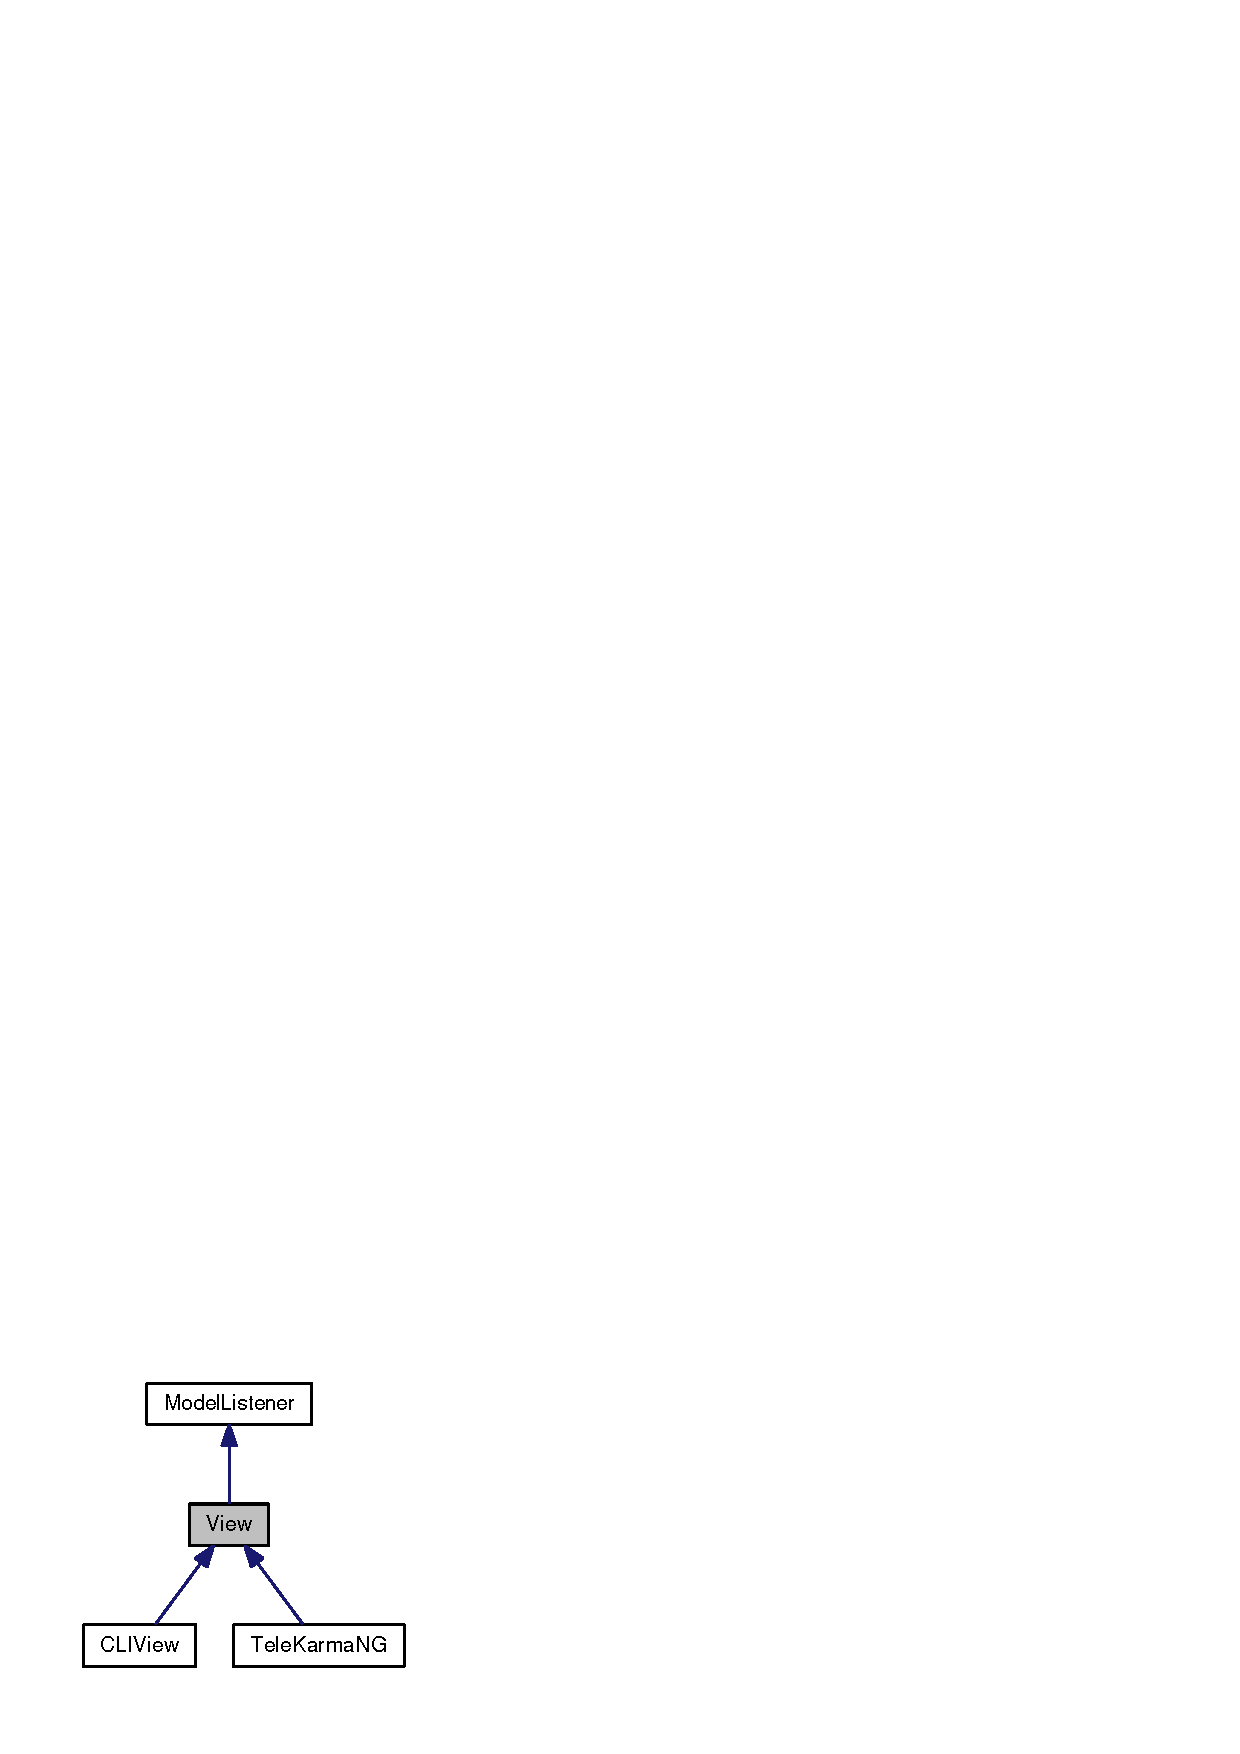
\includegraphics[width=198pt]{classView__inherit__graph}
\end{center}
\end{figure}
Collaboration diagram for View:\nopagebreak
\begin{figure}[H]
\begin{center}
\leavevmode

\includegraphics[width=250pt]{classView__coll__graph}
\end{center}
\end{figure}
\subsection*{Public Member Functions}
\begin{CompactItemize}
\item 
\hyperlink{classView_44ad60a768422d3fa8fbd7576950080a}{View} ()
\begin{CompactList}\small\item\em Default constructor. \item\end{CompactList}\item 
virtual \hyperlink{classView_a02a820358e1a7bf7e34d205212ae8f3}{$\sim$View} ()
\begin{CompactList}\small\item\em Virtual destructor, does nothing. \item\end{CompactList}\item 
virtual void \hyperlink{classView_92a0d9fd64b52e7f85d45c46c28a6546}{OnStateChange} ()
\begin{CompactList}\small\item\em Implementation of \hyperlink{classModelListener}{ModelListener}. \item\end{CompactList}\item 
virtual \hyperlink{classState}{State} $\ast$ \hyperlink{classView_b766758f8cf0667f20305f5b52cbe64e}{GetState} ()
\begin{CompactList}\small\item\em Returns the current \hyperlink{classState}{State} of the \hyperlink{classModel}{Model}. \item\end{CompactList}\item 
virtual \hyperlink{classState}{State} $\ast$ \hyperlink{classView_8d0521fb0bd96564906deab7fb58d411}{DequeueState} ()
\begin{CompactList}\small\item\em Dequeues a state from the model and returns it. \item\end{CompactList}\item 
virtual void \hyperlink{classView_cb2535000de204a5e4202c6ecce64666}{DoAction} (\hyperlink{classAction}{Action} $\ast$action)
\begin{CompactList}\small\item\em Enqueues an \hyperlink{classAction}{Action} in the \hyperlink{classModel}{Model}. \item\end{CompactList}\end{CompactItemize}
\subsection*{Protected Attributes}
\begin{CompactItemize}
\item 
\hyperlink{classModel}{Model} $\ast$ \hyperlink{classView_f9f5eea17223c374879af02bd02dfdfb}{model}
\begin{CompactList}\small\item\em The model used by the view. \item\end{CompactList}\item 
\hyperlink{classController}{Controller} $\ast$ \hyperlink{classView_e097997e36de3c065f600e768e62c249}{controller}
\begin{CompactList}\small\item\em The controller used by the view. \item\end{CompactList}\end{CompactItemize}


\subsection{Detailed Description}
Abstract superclass for all \hyperlink{classTeleKarma}{TeleKarma} views. 

Subclass this class to create a new view. 

\subsection{Constructor \& Destructor Documentation}
\hypertarget{classView_44ad60a768422d3fa8fbd7576950080a}{
\index{View@{View}!View@{View}}
\index{View@{View}!View@{View}}
\subsubsection[{View}]{\setlength{\rightskip}{0pt plus 5cm}View::View ()\hspace{0.3cm}{\tt  \mbox{[}inline\mbox{]}}}}
\label{classView_44ad60a768422d3fa8fbd7576950080a}


Default constructor. 

Initializes controller and model pointers to NULL. Note that subclasses are responsible for instantiating an appropriate model and controller. \hypertarget{classView_a02a820358e1a7bf7e34d205212ae8f3}{
\index{View@{View}!$\sim$View@{$\sim$View}}
\index{$\sim$View@{$\sim$View}!View@{View}}
\subsubsection[{$\sim$View}]{\setlength{\rightskip}{0pt plus 5cm}virtual View::$\sim$View ()\hspace{0.3cm}{\tt  \mbox{[}inline, virtual\mbox{]}}}}
\label{classView_a02a820358e1a7bf7e34d205212ae8f3}


Virtual destructor, does nothing. 



\subsection{Member Function Documentation}
\hypertarget{classView_8d0521fb0bd96564906deab7fb58d411}{
\index{View@{View}!DequeueState@{DequeueState}}
\index{DequeueState@{DequeueState}!View@{View}}
\subsubsection[{DequeueState}]{\setlength{\rightskip}{0pt plus 5cm}{\bf State} $\ast$ View::DequeueState ()\hspace{0.3cm}{\tt  \mbox{[}virtual\mbox{]}}}}
\label{classView_8d0521fb0bd96564906deab7fb58d411}


Dequeues a state from the model and returns it. 

\begin{Desc}
\item[Returns:]a pointer to an instance of a state that the caller is responsible for deleting, or NULL if the there have already been at least as many \hyperlink{classModel_a92abd0332df9f768033423b0cd8b3ae}{calls as  Model\#SetState(State $\ast$)} calls. \end{Desc}
\hypertarget{classView_cb2535000de204a5e4202c6ecce64666}{
\index{View@{View}!DoAction@{DoAction}}
\index{DoAction@{DoAction}!View@{View}}
\subsubsection[{DoAction}]{\setlength{\rightskip}{0pt plus 5cm}void View::DoAction ({\bf Action} $\ast$ {\em action})\hspace{0.3cm}{\tt  \mbox{[}virtual\mbox{]}}}}
\label{classView_cb2535000de204a5e4202c6ecce64666}


Enqueues an \hyperlink{classAction}{Action} in the \hyperlink{classModel}{Model}. 

Caller should not modify the \hyperlink{classAction}{Action} after enqueuing it. \begin{Desc}
\item[Parameters:]
\begin{description}
\item[{\em action}]an action for the controller to take. \end{description}
\end{Desc}
\hypertarget{classView_b766758f8cf0667f20305f5b52cbe64e}{
\index{View@{View}!GetState@{GetState}}
\index{GetState@{GetState}!View@{View}}
\subsubsection[{GetState}]{\setlength{\rightskip}{0pt plus 5cm}{\bf State} $\ast$ View::GetState ()\hspace{0.3cm}{\tt  \mbox{[}virtual\mbox{]}}}}
\label{classView_b766758f8cf0667f20305f5b52cbe64e}


Returns the current \hyperlink{classState}{State} of the \hyperlink{classModel}{Model}. 

\begin{Desc}
\item[Returns:]the current \hyperlink{classState}{State} of the \hyperlink{classModel}{Model}. \end{Desc}
\hypertarget{classView_92a0d9fd64b52e7f85d45c46c28a6546}{
\index{View@{View}!OnStateChange@{OnStateChange}}
\index{OnStateChange@{OnStateChange}!View@{View}}
\subsubsection[{OnStateChange}]{\setlength{\rightskip}{0pt plus 5cm}virtual void View::OnStateChange ()\hspace{0.3cm}{\tt  \mbox{[}inline, virtual\mbox{]}}}}
\label{classView_92a0d9fd64b52e7f85d45c46c28a6546}


Implementation of \hyperlink{classModelListener}{ModelListener}. 

Does nothing. Subclasses may or may not wish to reimplement this method. 

Implements \hyperlink{classModelListener_63070a6f75480904846b7cfc6389aa4c}{ModelListener}.

Reimplemented in \hyperlink{classTeleKarmaNG_ce1e8d62f3e1d586e2aa5d2012c9a766}{TeleKarmaNG}.

\subsection{Member Data Documentation}
\hypertarget{classView_e097997e36de3c065f600e768e62c249}{
\index{View@{View}!controller@{controller}}
\index{controller@{controller}!View@{View}}
\subsubsection[{controller}]{\setlength{\rightskip}{0pt plus 5cm}{\bf Controller}$\ast$ {\bf View::controller}\hspace{0.3cm}{\tt  \mbox{[}protected\mbox{]}}}}
\label{classView_e097997e36de3c065f600e768e62c249}


The controller used by the view. 

Subclasses are responsible for instantiation. \hypertarget{classView_f9f5eea17223c374879af02bd02dfdfb}{
\index{View@{View}!model@{model}}
\index{model@{model}!View@{View}}
\subsubsection[{model}]{\setlength{\rightskip}{0pt plus 5cm}{\bf Model}$\ast$ {\bf View::model}\hspace{0.3cm}{\tt  \mbox{[}protected\mbox{]}}}}
\label{classView_f9f5eea17223c374879af02bd02dfdfb}


The model used by the view. 

Subclasses are responsible for instantiation. 

The documentation for this class was generated from the following files:\begin{CompactItemize}
\item 
\hyperlink{view_8h}{view.h}\item 
\hyperlink{view_8cpp}{view.cpp}\end{CompactItemize}

\hypertarget{classwxDialPadClosedEvent}{
\section{wxDialPadClosedEvent Class Reference}
\label{classwxDialPadClosedEvent}\index{wxDialPadClosedEvent@{wxDialPadClosedEvent}}
}
{\tt \#include $<$gui.h$>$}

\subsection*{Public Member Functions}
\begin{CompactItemize}
\item 
\hyperlink{classwxDialPadClosedEvent_2fc1dd8d8309caacf0c74771356d3743}{wxDialPadClosedEvent} (wxObject $\ast$origin)
\item 
virtual wxEvent $\ast$ \hyperlink{classwxDialPadClosedEvent_e4f9e1196ee65a651b572c285dcdd75e}{Clone} ()
\end{CompactItemize}


\subsection{Constructor \& Destructor Documentation}
\hypertarget{classwxDialPadClosedEvent_2fc1dd8d8309caacf0c74771356d3743}{
\index{wxDialPadClosedEvent@{wxDialPadClosedEvent}!wxDialPadClosedEvent@{wxDialPadClosedEvent}}
\index{wxDialPadClosedEvent@{wxDialPadClosedEvent}!wxDialPadClosedEvent@{wxDialPadClosedEvent}}
\subsubsection[{wxDialPadClosedEvent}]{\setlength{\rightskip}{0pt plus 5cm}wxDialPadClosedEvent::wxDialPadClosedEvent (wxObject $\ast$ {\em origin})}}
\label{classwxDialPadClosedEvent_2fc1dd8d8309caacf0c74771356d3743}




\subsection{Member Function Documentation}
\hypertarget{classwxDialPadClosedEvent_e4f9e1196ee65a651b572c285dcdd75e}{
\index{wxDialPadClosedEvent@{wxDialPadClosedEvent}!Clone@{Clone}}
\index{Clone@{Clone}!wxDialPadClosedEvent@{wxDialPadClosedEvent}}
\subsubsection[{Clone}]{\setlength{\rightskip}{0pt plus 5cm}wxEvent $\ast$ wxDialPadClosedEvent::Clone ()\hspace{0.3cm}{\tt  \mbox{[}virtual\mbox{]}}}}
\label{classwxDialPadClosedEvent_e4f9e1196ee65a651b572c285dcdd75e}




The documentation for this class was generated from the following files:\begin{CompactItemize}
\item 
\hyperlink{gui_8h}{gui.h}\item 
\hyperlink{gui_8cpp}{gui.cpp}\end{CompactItemize}

\hypertarget{classwxRegisterDialogClosedEvent}{
\section{wxRegisterDialogClosedEvent Class Reference}
\label{classwxRegisterDialogClosedEvent}\index{wxRegisterDialogClosedEvent@{wxRegisterDialogClosedEvent}}
}
{\tt \#include $<$gui.h$>$}

\subsection*{Public Member Functions}
\begin{CompactItemize}
\item 
\hyperlink{classwxRegisterDialogClosedEvent_278f2b13aa9b5768d3b0f21de2ef6962}{wxRegisterDialogClosedEvent} (wxObject $\ast$origin)
\item 
virtual wxEvent $\ast$ \hyperlink{classwxRegisterDialogClosedEvent_f49e7ab28e7de6b258c2fa774ab5a210}{Clone} ()
\end{CompactItemize}


\subsection{Constructor \& Destructor Documentation}
\hypertarget{classwxRegisterDialogClosedEvent_278f2b13aa9b5768d3b0f21de2ef6962}{
\index{wxRegisterDialogClosedEvent@{wxRegisterDialogClosedEvent}!wxRegisterDialogClosedEvent@{wxRegisterDialogClosedEvent}}
\index{wxRegisterDialogClosedEvent@{wxRegisterDialogClosedEvent}!wxRegisterDialogClosedEvent@{wxRegisterDialogClosedEvent}}
\subsubsection[{wxRegisterDialogClosedEvent}]{\setlength{\rightskip}{0pt plus 5cm}wxRegisterDialogClosedEvent::wxRegisterDialogClosedEvent (wxObject $\ast$ {\em origin})}}
\label{classwxRegisterDialogClosedEvent_278f2b13aa9b5768d3b0f21de2ef6962}




\subsection{Member Function Documentation}
\hypertarget{classwxRegisterDialogClosedEvent_f49e7ab28e7de6b258c2fa774ab5a210}{
\index{wxRegisterDialogClosedEvent@{wxRegisterDialogClosedEvent}!Clone@{Clone}}
\index{Clone@{Clone}!wxRegisterDialogClosedEvent@{wxRegisterDialogClosedEvent}}
\subsubsection[{Clone}]{\setlength{\rightskip}{0pt plus 5cm}wxEvent $\ast$ wxRegisterDialogClosedEvent::Clone ()\hspace{0.3cm}{\tt  \mbox{[}virtual\mbox{]}}}}
\label{classwxRegisterDialogClosedEvent_f49e7ab28e7de6b258c2fa774ab5a210}




The documentation for this class was generated from the following files:\begin{CompactItemize}
\item 
\hyperlink{gui_8h}{gui.h}\item 
\hyperlink{gui_8cpp}{gui.cpp}\end{CompactItemize}

\hypertarget{classwxStateChangeEvent}{
\section{wxStateChangeEvent Class Reference}
\label{classwxStateChangeEvent}\index{wxStateChangeEvent@{wxStateChangeEvent}}
}
{\tt \#include $<$gui.h$>$}

\subsection*{Public Member Functions}
\begin{CompactItemize}
\item 
\hyperlink{classwxStateChangeEvent_dee1018c458a03a33ee5b4fedc12c9a0}{wxStateChangeEvent} (wxObject $\ast$origin)
\item 
virtual wxEvent $\ast$ \hyperlink{classwxStateChangeEvent_92d5b5b4e174eeb2532cd44711ee4c3a}{Clone} ()
\end{CompactItemize}


\subsection{Constructor \& Destructor Documentation}
\hypertarget{classwxStateChangeEvent_dee1018c458a03a33ee5b4fedc12c9a0}{
\index{wxStateChangeEvent@{wxStateChangeEvent}!wxStateChangeEvent@{wxStateChangeEvent}}
\index{wxStateChangeEvent@{wxStateChangeEvent}!wxStateChangeEvent@{wxStateChangeEvent}}
\subsubsection[{wxStateChangeEvent}]{\setlength{\rightskip}{0pt plus 5cm}wxStateChangeEvent::wxStateChangeEvent (wxObject $\ast$ {\em origin})}}
\label{classwxStateChangeEvent_dee1018c458a03a33ee5b4fedc12c9a0}




\subsection{Member Function Documentation}
\hypertarget{classwxStateChangeEvent_92d5b5b4e174eeb2532cd44711ee4c3a}{
\index{wxStateChangeEvent@{wxStateChangeEvent}!Clone@{Clone}}
\index{Clone@{Clone}!wxStateChangeEvent@{wxStateChangeEvent}}
\subsubsection[{Clone}]{\setlength{\rightskip}{0pt plus 5cm}wxEvent $\ast$ wxStateChangeEvent::Clone ()\hspace{0.3cm}{\tt  \mbox{[}virtual\mbox{]}}}}
\label{classwxStateChangeEvent_92d5b5b4e174eeb2532cd44711ee4c3a}




The documentation for this class was generated from the following files:\begin{CompactItemize}
\item 
\hyperlink{gui_8h}{gui.h}\item 
\hyperlink{gui_8cpp}{gui.cpp}\end{CompactItemize}

\chapter{File Documentation}
\hypertarget{account_8cpp}{
\section{account.cpp File Reference}
\label{account_8cpp}\index{account.cpp@{account.cpp}}
}
{\tt \#include $<$ptlib.h$>$}\par
{\tt \#include $<$ptlib/textfile.h$>$}\par
{\tt \#include $<$ptlib/filepath.h$>$}\par
{\tt \#include $<$ptlib/channel.h$>$}\par
{\tt \#include \char`\"{}account.h\char`\"{}}\par


Include dependency graph for account.cpp:\nopagebreak
\begin{figure}[H]
\begin{center}
\leavevmode

\includegraphics[width=225pt]{account_8cpp__incl}
\end{center}
\end{figure}

\hypertarget{account_8h}{
\section{account.h File Reference}
\label{account_8h}\index{account.h@{account.h}}
}


This graph shows which files directly or indirectly include this file:\nopagebreak
\begin{figure}[H]
\begin{center}
\leavevmode
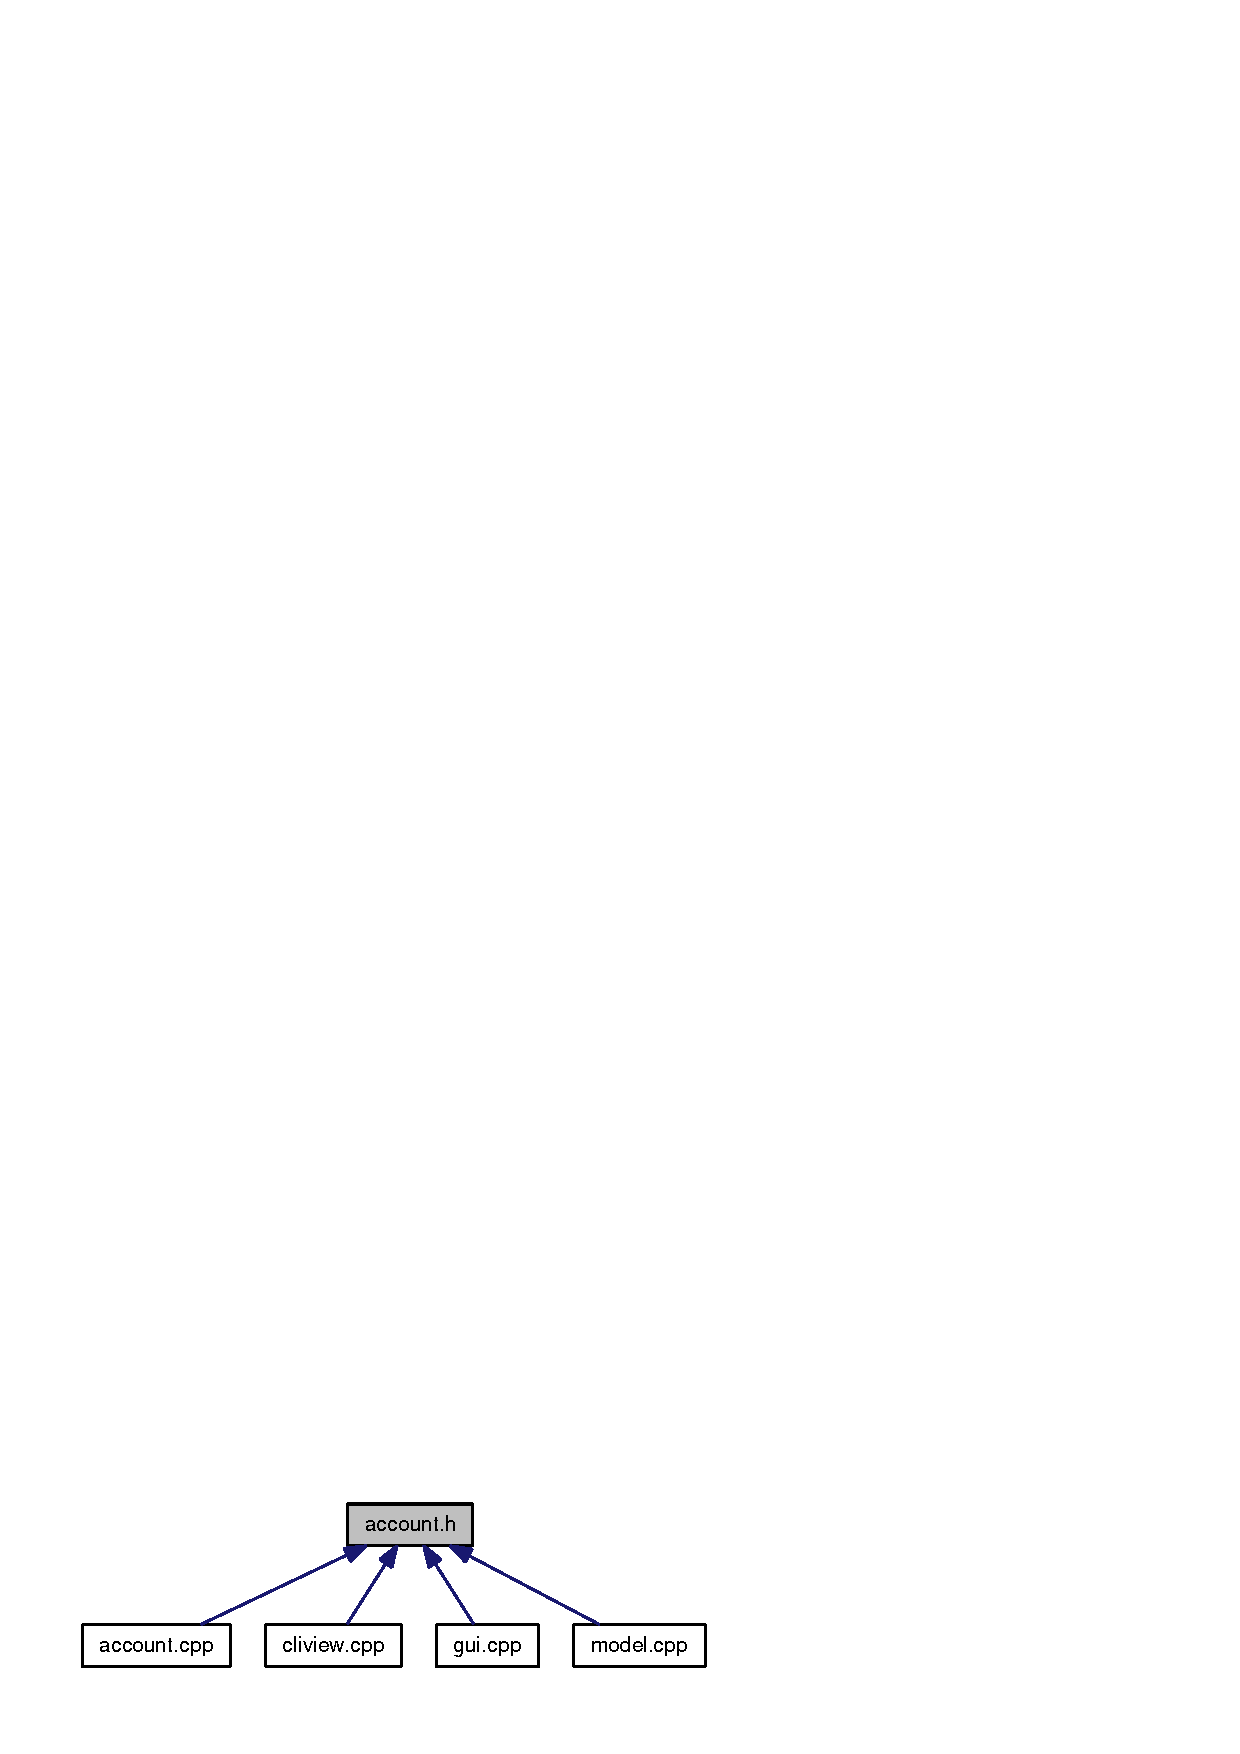
\includegraphics[width=171pt]{account_8h__dep__incl}
\end{center}
\end{figure}
\subsection*{Classes}
\begin{CompactItemize}
\item 
class \hyperlink{classAccount}{Account}
\begin{CompactList}\small\item\em Represents a user's account with a SIP service provider. \item\end{CompactList}\item 
class \hyperlink{classAccountList}{AccountList}
\begin{CompactList}\small\item\em Represents a persistant list of SIP service provider accounts. \item\end{CompactList}\end{CompactItemize}
\subsection*{Defines}
\begin{CompactItemize}
\item 
\#define \hyperlink{account_8h_c81e4476f50e41e8a77c416a584b65fd}{DEFAULT\_\-STUN\_\-SERVER}~\char`\"{}stun.ekiga.net\char`\"{}
\end{CompactItemize}


\subsection{Define Documentation}
\hypertarget{account_8h_c81e4476f50e41e8a77c416a584b65fd}{
\index{account.h@{account.h}!DEFAULT\_\-STUN\_\-SERVER@{DEFAULT\_\-STUN\_\-SERVER}}
\index{DEFAULT\_\-STUN\_\-SERVER@{DEFAULT\_\-STUN\_\-SERVER}!account.h@{account.h}}
\subsubsection[{DEFAULT\_\-STUN\_\-SERVER}]{\setlength{\rightskip}{0pt plus 5cm}\#define DEFAULT\_\-STUN\_\-SERVER~\char`\"{}stun.ekiga.net\char`\"{}}}
\label{account_8h_c81e4476f50e41e8a77c416a584b65fd}



\hypertarget{action_8cpp}{
\section{action.cpp File Reference}
\label{action_8cpp}\index{action.cpp@{action.cpp}}
}
{\tt \#include $<$iostream$>$}\par
{\tt \#include $<$ptlib.h$>$}\par
{\tt \#include \char`\"{}action.h\char`\"{}}\par


Include dependency graph for action.cpp:\nopagebreak
\begin{figure}[H]
\begin{center}
\leavevmode
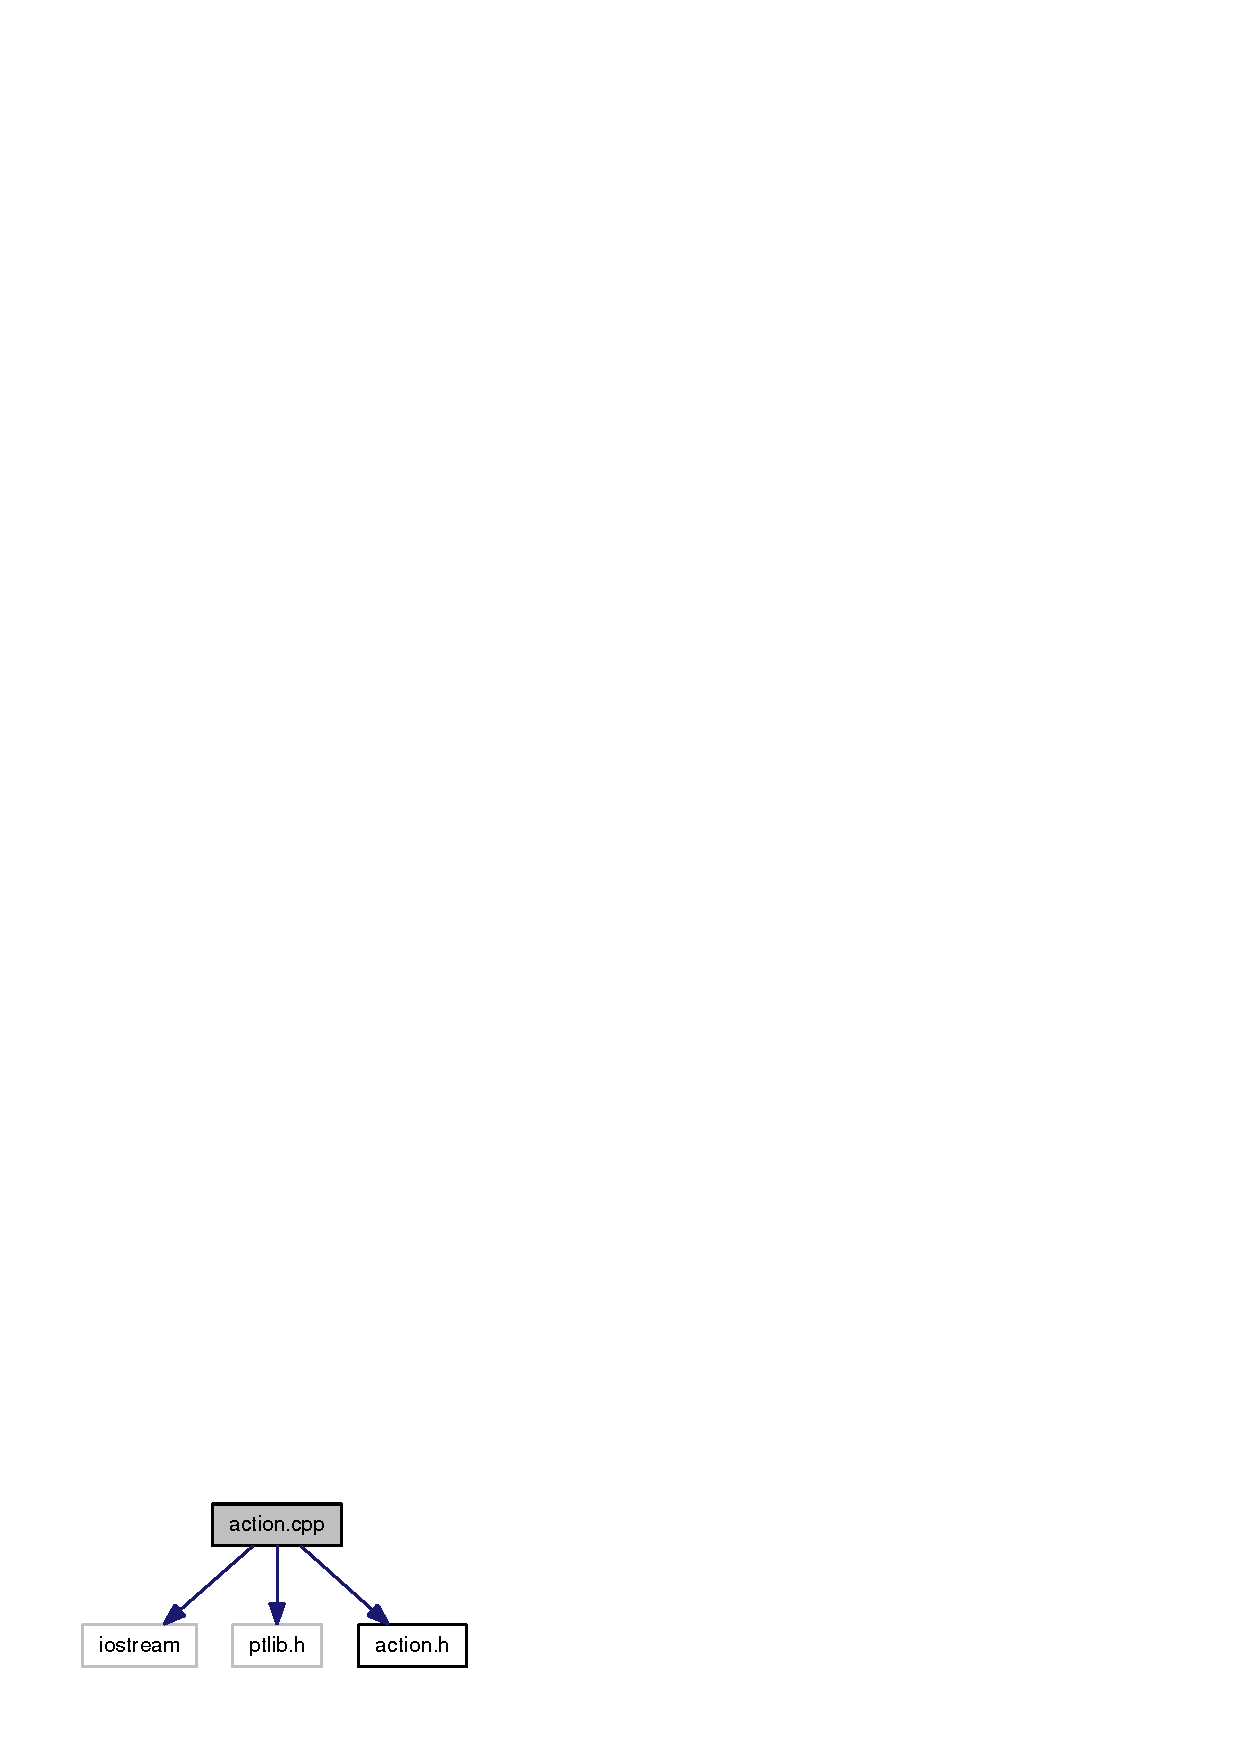
\includegraphics[width=114pt]{action_8cpp__incl}
\end{center}
\end{figure}

\hypertarget{action_8h}{
\section{action.h File Reference}
\label{action_8h}\index{action.h@{action.h}}
}


This graph shows which files directly or indirectly include this file:\nopagebreak
\begin{figure}[H]
\begin{center}
\leavevmode

\includegraphics[width=216pt]{action_8h__dep__incl}
\end{center}
\end{figure}
\subsection*{Classes}
\begin{CompactItemize}
\item 
class \hyperlink{classAction}{Action}
\item 
class \hyperlink{classInitializeAction}{InitializeAction}
\item 
class \hyperlink{classRegisterAction}{RegisterAction}
\item 
class \hyperlink{classDialAction}{DialAction}
\item 
class \hyperlink{classHoldAction}{HoldAction}
\item 
class \hyperlink{classAutoHoldAction}{AutoHoldAction}
\item 
class \hyperlink{classRetrieveAction}{RetrieveAction}
\item 
class \hyperlink{classSendToneAction}{SendToneAction}
\item 
class \hyperlink{classDisconnectAction}{DisconnectAction}
\item 
class \hyperlink{classQuitAction}{QuitAction}
\item 
class \hyperlink{classPlaySoundAction}{PlaySoundAction}
\end{CompactItemize}
\subsection*{Enumerations}
\begin{CompactItemize}
\item 
enum \hyperlink{action_8h_3664bc98cf666c3d88d23f3fd5d9251c}{ActionID} \{ \par
\hyperlink{action_8h_3664bc98cf666c3d88d23f3fd5d9251cf809fb89fb370ef60de1fbc4cac2cf0a}{ACTION\_\-INITIALIZE}, 
\hyperlink{action_8h_3664bc98cf666c3d88d23f3fd5d9251c3e50e2e73ddcbc0224f21160587db4dc}{ACTION\_\-REGISTER}, 
\hyperlink{action_8h_3664bc98cf666c3d88d23f3fd5d9251c719829d27c791e98793a0c8d59915e2d}{ACTION\_\-DIAL}, 
\hyperlink{action_8h_3664bc98cf666c3d88d23f3fd5d9251c6ed7945499359e8e42d4525fced49046}{ACTION\_\-HOLD}, 
\par
\hyperlink{action_8h_3664bc98cf666c3d88d23f3fd5d9251c1c5391634cbc567c75884abbd8167253}{ACTION\_\-AUTOHOLD}, 
\hyperlink{action_8h_3664bc98cf666c3d88d23f3fd5d9251cb44b14ad49758f5c9428763c8e7846d2}{ACTION\_\-MUTE}, 
\hyperlink{action_8h_3664bc98cf666c3d88d23f3fd5d9251cd435905789793573e617b2262e8f10a7}{ACTION\_\-RETRIEVE}, 
\hyperlink{action_8h_3664bc98cf666c3d88d23f3fd5d9251c9ee92e670ed2a457721f3a3d36f91586}{ACTION\_\-SEND\_\-TONE}, 
\par
\hyperlink{action_8h_3664bc98cf666c3d88d23f3fd5d9251c0adc282807501d17a976a2f62d736946}{ACTION\_\-DISCONNECT}, 
\hyperlink{action_8h_3664bc98cf666c3d88d23f3fd5d9251cddd63f860ba8647fd5cf8856fe83fab3}{ACTION\_\-QUIT}, 
\hyperlink{action_8h_3664bc98cf666c3d88d23f3fd5d9251c0f1323e5e7dc4a07f4acea09dbb8522a}{ACTION\_\-PLAY\_\-SOUND}
 \}
\end{CompactItemize}


\subsection{Enumeration Type Documentation}
\hypertarget{action_8h_3664bc98cf666c3d88d23f3fd5d9251c}{
\index{action.h@{action.h}!ActionID@{ActionID}}
\index{ActionID@{ActionID}!action.h@{action.h}}
\subsubsection[{ActionID}]{\setlength{\rightskip}{0pt plus 5cm}enum {\bf ActionID}}}
\label{action_8h_3664bc98cf666c3d88d23f3fd5d9251c}


\begin{Desc}
\item[Enumerator: ]\par
\begin{description}
\index{ACTION\_\-INITIALIZE@{ACTION\_\-INITIALIZE}!action.h@{action.h}}\index{action.h@{action.h}!ACTION\_\-INITIALIZE@{ACTION\_\-INITIALIZE}}\item[{\em 
\hypertarget{action_8h_3664bc98cf666c3d88d23f3fd5d9251cf809fb89fb370ef60de1fbc4cac2cf0a}{
ACTION\_\-INITIALIZE}
\label{action_8h_3664bc98cf666c3d88d23f3fd5d9251cf809fb89fb370ef60de1fbc4cac2cf0a}
}]\index{ACTION\_\-REGISTER@{ACTION\_\-REGISTER}!action.h@{action.h}}\index{action.h@{action.h}!ACTION\_\-REGISTER@{ACTION\_\-REGISTER}}\item[{\em 
\hypertarget{action_8h_3664bc98cf666c3d88d23f3fd5d9251c3e50e2e73ddcbc0224f21160587db4dc}{
ACTION\_\-REGISTER}
\label{action_8h_3664bc98cf666c3d88d23f3fd5d9251c3e50e2e73ddcbc0224f21160587db4dc}
}]\index{ACTION\_\-DIAL@{ACTION\_\-DIAL}!action.h@{action.h}}\index{action.h@{action.h}!ACTION\_\-DIAL@{ACTION\_\-DIAL}}\item[{\em 
\hypertarget{action_8h_3664bc98cf666c3d88d23f3fd5d9251c719829d27c791e98793a0c8d59915e2d}{
ACTION\_\-DIAL}
\label{action_8h_3664bc98cf666c3d88d23f3fd5d9251c719829d27c791e98793a0c8d59915e2d}
}]\index{ACTION\_\-HOLD@{ACTION\_\-HOLD}!action.h@{action.h}}\index{action.h@{action.h}!ACTION\_\-HOLD@{ACTION\_\-HOLD}}\item[{\em 
\hypertarget{action_8h_3664bc98cf666c3d88d23f3fd5d9251c6ed7945499359e8e42d4525fced49046}{
ACTION\_\-HOLD}
\label{action_8h_3664bc98cf666c3d88d23f3fd5d9251c6ed7945499359e8e42d4525fced49046}
}]\index{ACTION\_\-AUTOHOLD@{ACTION\_\-AUTOHOLD}!action.h@{action.h}}\index{action.h@{action.h}!ACTION\_\-AUTOHOLD@{ACTION\_\-AUTOHOLD}}\item[{\em 
\hypertarget{action_8h_3664bc98cf666c3d88d23f3fd5d9251c1c5391634cbc567c75884abbd8167253}{
ACTION\_\-AUTOHOLD}
\label{action_8h_3664bc98cf666c3d88d23f3fd5d9251c1c5391634cbc567c75884abbd8167253}
}]\index{ACTION\_\-MUTE@{ACTION\_\-MUTE}!action.h@{action.h}}\index{action.h@{action.h}!ACTION\_\-MUTE@{ACTION\_\-MUTE}}\item[{\em 
\hypertarget{action_8h_3664bc98cf666c3d88d23f3fd5d9251cb44b14ad49758f5c9428763c8e7846d2}{
ACTION\_\-MUTE}
\label{action_8h_3664bc98cf666c3d88d23f3fd5d9251cb44b14ad49758f5c9428763c8e7846d2}
}]\index{ACTION\_\-RETRIEVE@{ACTION\_\-RETRIEVE}!action.h@{action.h}}\index{action.h@{action.h}!ACTION\_\-RETRIEVE@{ACTION\_\-RETRIEVE}}\item[{\em 
\hypertarget{action_8h_3664bc98cf666c3d88d23f3fd5d9251cd435905789793573e617b2262e8f10a7}{
ACTION\_\-RETRIEVE}
\label{action_8h_3664bc98cf666c3d88d23f3fd5d9251cd435905789793573e617b2262e8f10a7}
}]\index{ACTION\_\-SEND\_\-TONE@{ACTION\_\-SEND\_\-TONE}!action.h@{action.h}}\index{action.h@{action.h}!ACTION\_\-SEND\_\-TONE@{ACTION\_\-SEND\_\-TONE}}\item[{\em 
\hypertarget{action_8h_3664bc98cf666c3d88d23f3fd5d9251c9ee92e670ed2a457721f3a3d36f91586}{
ACTION\_\-SEND\_\-TONE}
\label{action_8h_3664bc98cf666c3d88d23f3fd5d9251c9ee92e670ed2a457721f3a3d36f91586}
}]\index{ACTION\_\-DISCONNECT@{ACTION\_\-DISCONNECT}!action.h@{action.h}}\index{action.h@{action.h}!ACTION\_\-DISCONNECT@{ACTION\_\-DISCONNECT}}\item[{\em 
\hypertarget{action_8h_3664bc98cf666c3d88d23f3fd5d9251c0adc282807501d17a976a2f62d736946}{
ACTION\_\-DISCONNECT}
\label{action_8h_3664bc98cf666c3d88d23f3fd5d9251c0adc282807501d17a976a2f62d736946}
}]\index{ACTION\_\-QUIT@{ACTION\_\-QUIT}!action.h@{action.h}}\index{action.h@{action.h}!ACTION\_\-QUIT@{ACTION\_\-QUIT}}\item[{\em 
\hypertarget{action_8h_3664bc98cf666c3d88d23f3fd5d9251cddd63f860ba8647fd5cf8856fe83fab3}{
ACTION\_\-QUIT}
\label{action_8h_3664bc98cf666c3d88d23f3fd5d9251cddd63f860ba8647fd5cf8856fe83fab3}
}]\index{ACTION\_\-PLAY\_\-SOUND@{ACTION\_\-PLAY\_\-SOUND}!action.h@{action.h}}\index{action.h@{action.h}!ACTION\_\-PLAY\_\-SOUND@{ACTION\_\-PLAY\_\-SOUND}}\item[{\em 
\hypertarget{action_8h_3664bc98cf666c3d88d23f3fd5d9251c0f1323e5e7dc4a07f4acea09dbb8522a}{
ACTION\_\-PLAY\_\-SOUND}
\label{action_8h_3664bc98cf666c3d88d23f3fd5d9251c0f1323e5e7dc4a07f4acea09dbb8522a}
}]\end{description}
\end{Desc}


\hypertarget{clicontext_8cpp}{
\section{clicontext.cpp File Reference}
\label{clicontext_8cpp}\index{clicontext.cpp@{clicontext.cpp}}
}
{\tt \#include \char`\"{}clicontext.h\char`\"{}}\par


Include dependency graph for clicontext.cpp:\nopagebreak
\begin{figure}[H]
\begin{center}
\leavevmode
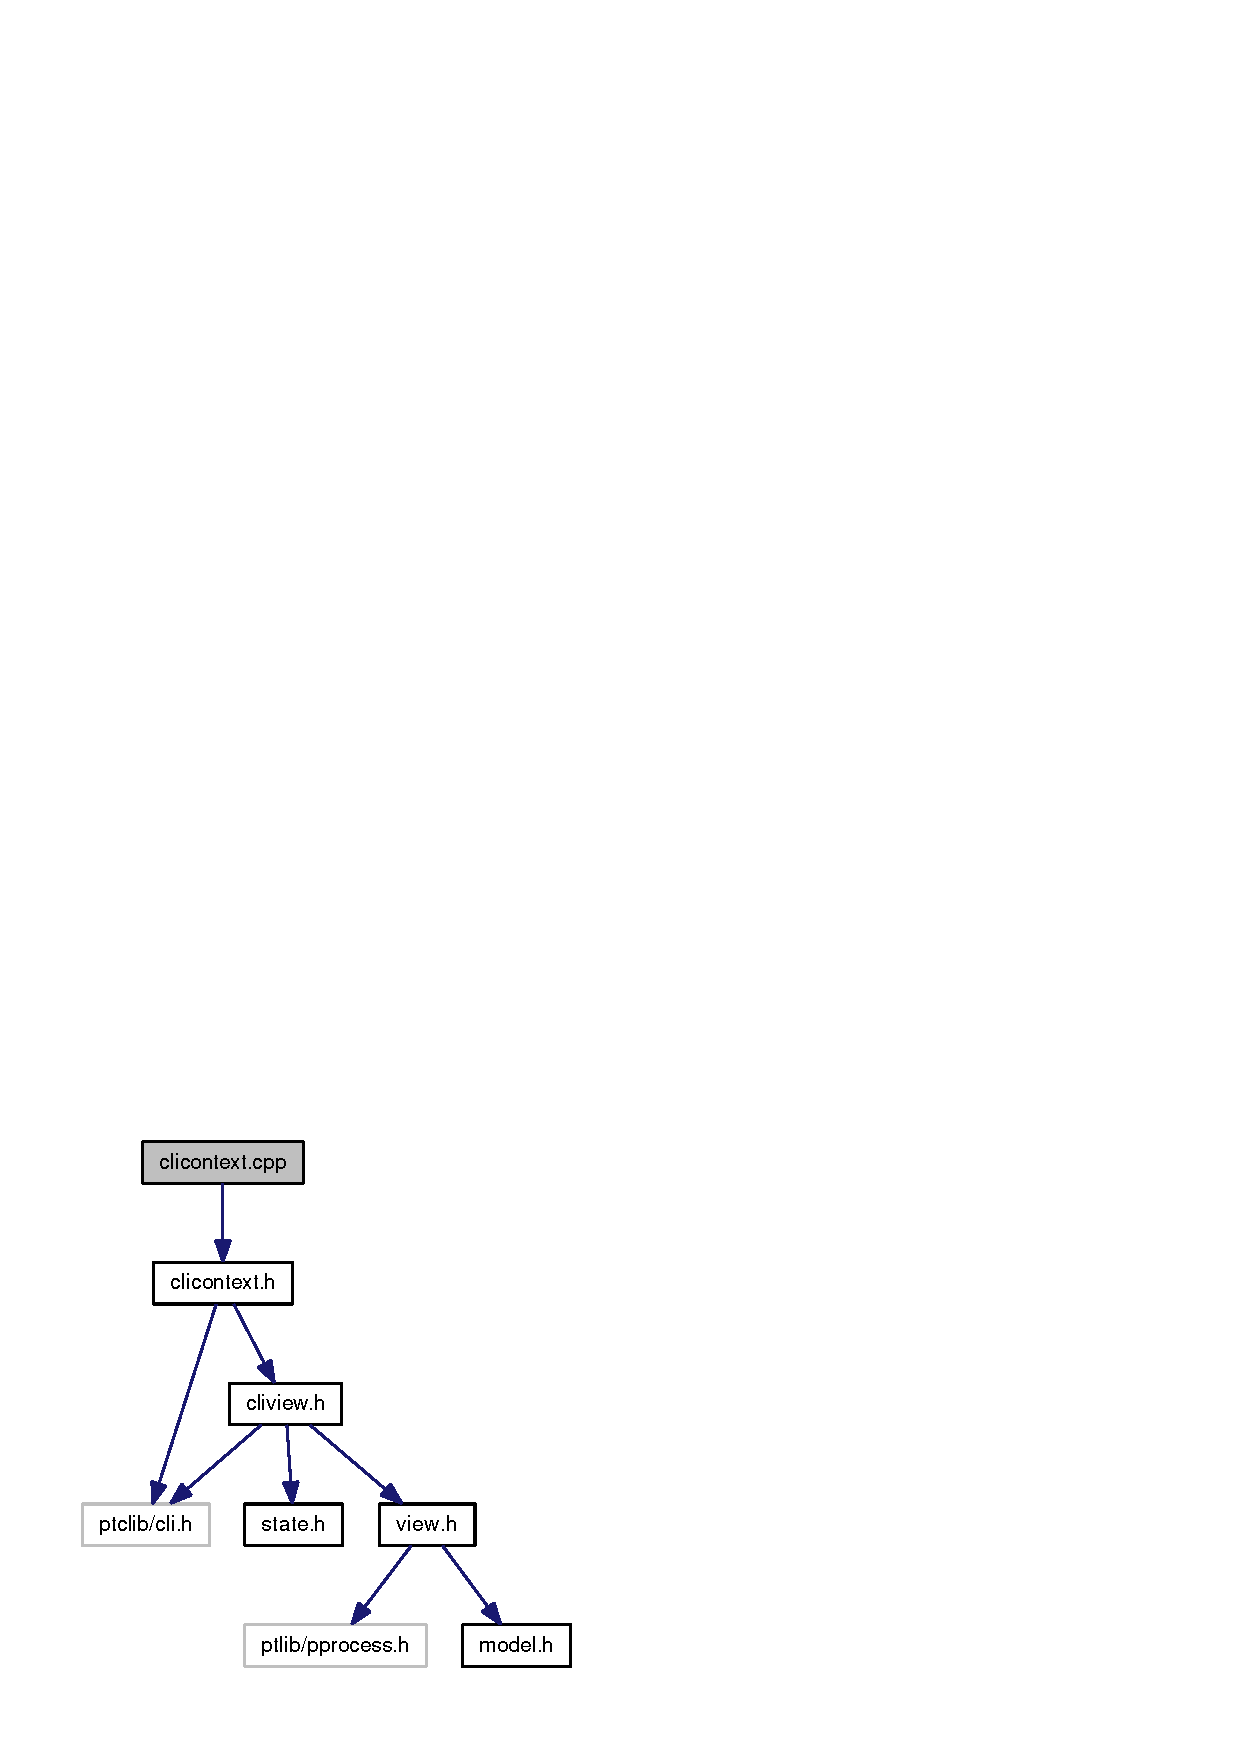
\includegraphics[width=139pt]{clicontext_8cpp__incl}
\end{center}
\end{figure}

\hypertarget{clicontext_8h}{
\section{clicontext.h File Reference}
\label{clicontext_8h}\index{clicontext.h@{clicontext.h}}
}
{\tt \#include $<$ptclib/cli.h$>$}\par
{\tt \#include \char`\"{}cliview.h\char`\"{}}\par


Include dependency graph for clicontext.h:\nopagebreak
\begin{figure}[H]
\begin{center}
\leavevmode

\includegraphics[width=139pt]{clicontext_8h__incl}
\end{center}
\end{figure}


This graph shows which files directly or indirectly include this file:\nopagebreak
\begin{figure}[H]
\begin{center}
\leavevmode
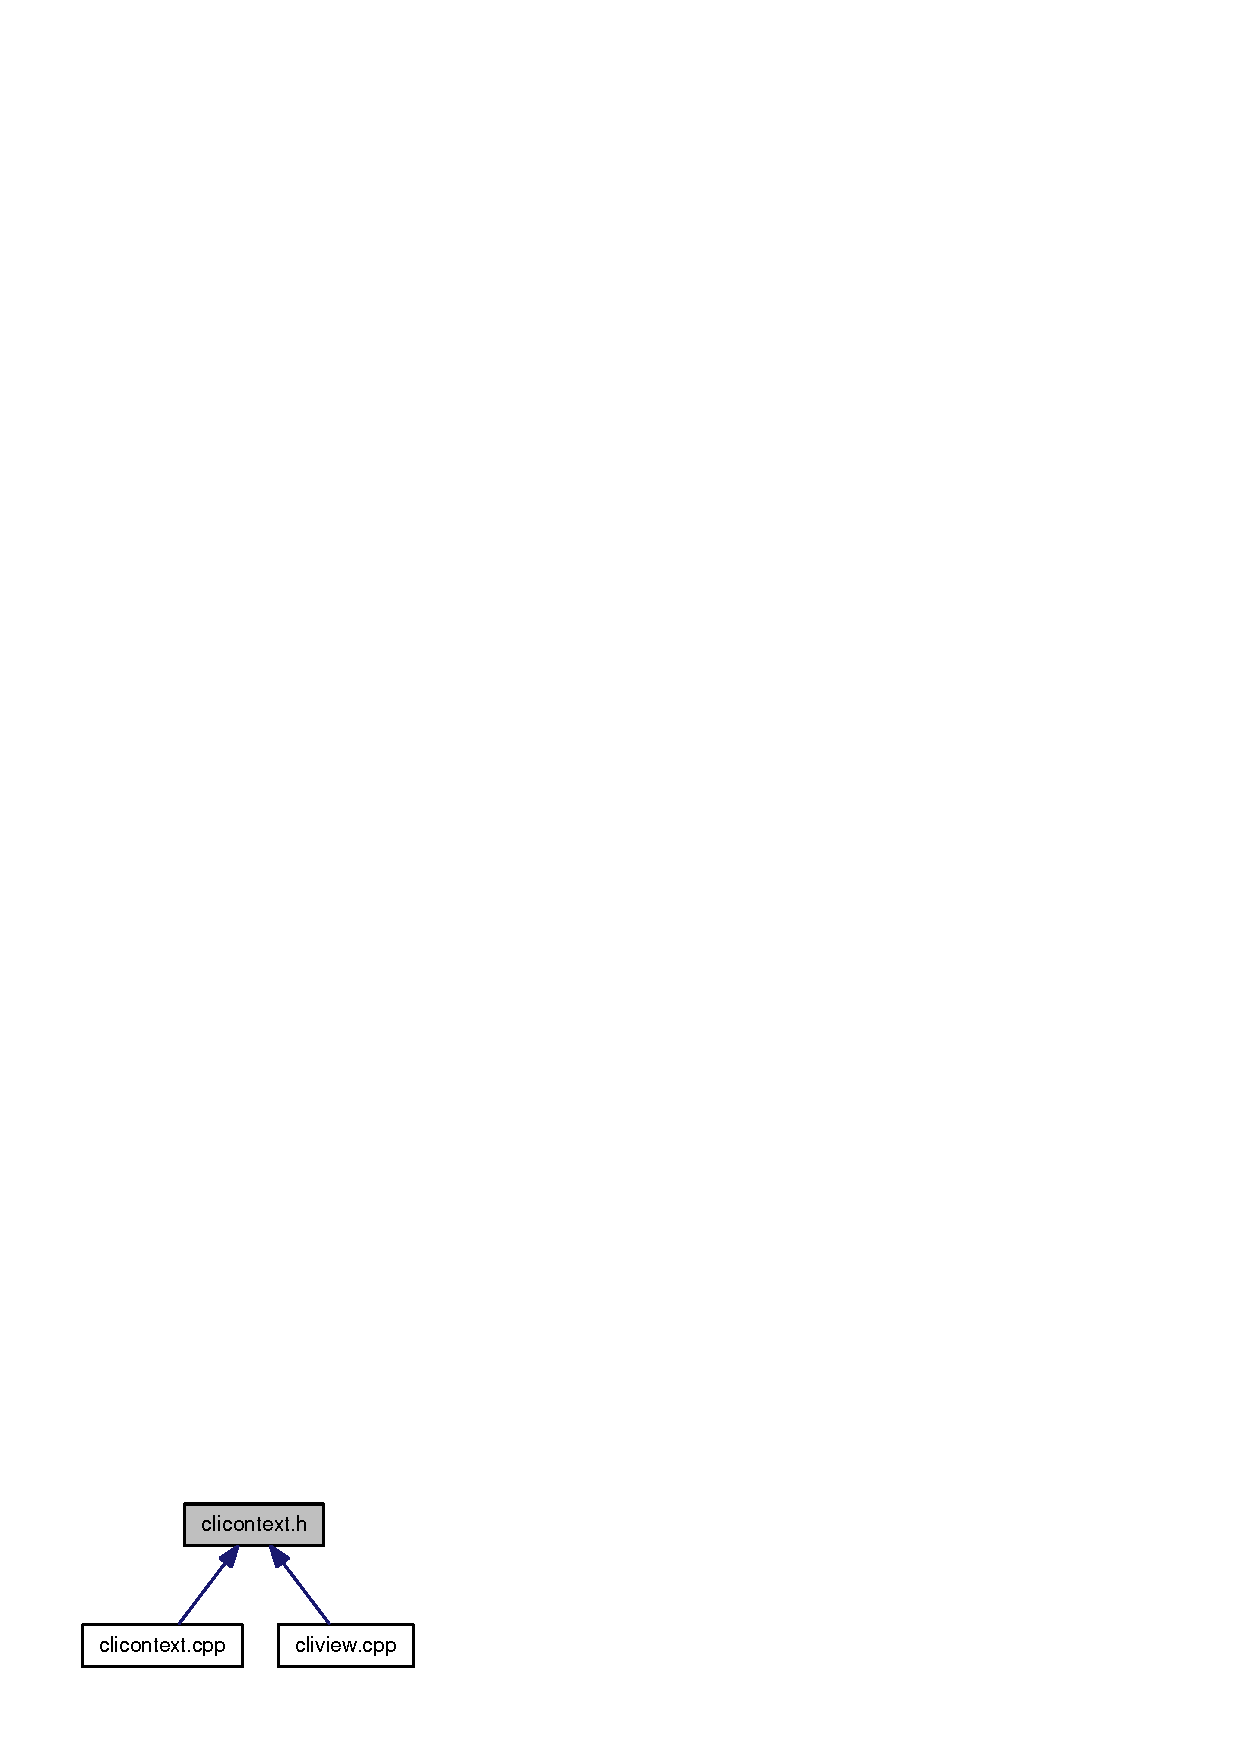
\includegraphics[width=101pt]{clicontext_8h__dep__incl}
\end{center}
\end{figure}
\subsection*{Classes}
\begin{CompactItemize}
\item 
class \hyperlink{classCLIContext}{CLIContext}
\end{CompactItemize}

\hypertarget{cliview_8cpp}{
\section{cliview.cpp File Reference}
\label{cliview_8cpp}\index{cliview.cpp@{cliview.cpp}}
}
{\tt \#include \char`\"{}cliview.h\char`\"{}}\par
{\tt \#include $<$ptlib/sound.h$>$}\par
{\tt \#include \char`\"{}action.h\char`\"{}}\par
{\tt \#include \char`\"{}account.h\char`\"{}}\par
{\tt \#include \char`\"{}clicontext.h\char`\"{}}\par
{\tt \#include \char`\"{}controller.h\char`\"{}}\par
{\tt \#include \char`\"{}model.h\char`\"{}}\par
{\tt \#include \char`\"{}state.h\char`\"{}}\par
{\tt \#include \char`\"{}telekarma.h\char`\"{}}\par


Include dependency graph for cliview.cpp:\nopagebreak
\begin{figure}[H]
\begin{center}
\leavevmode
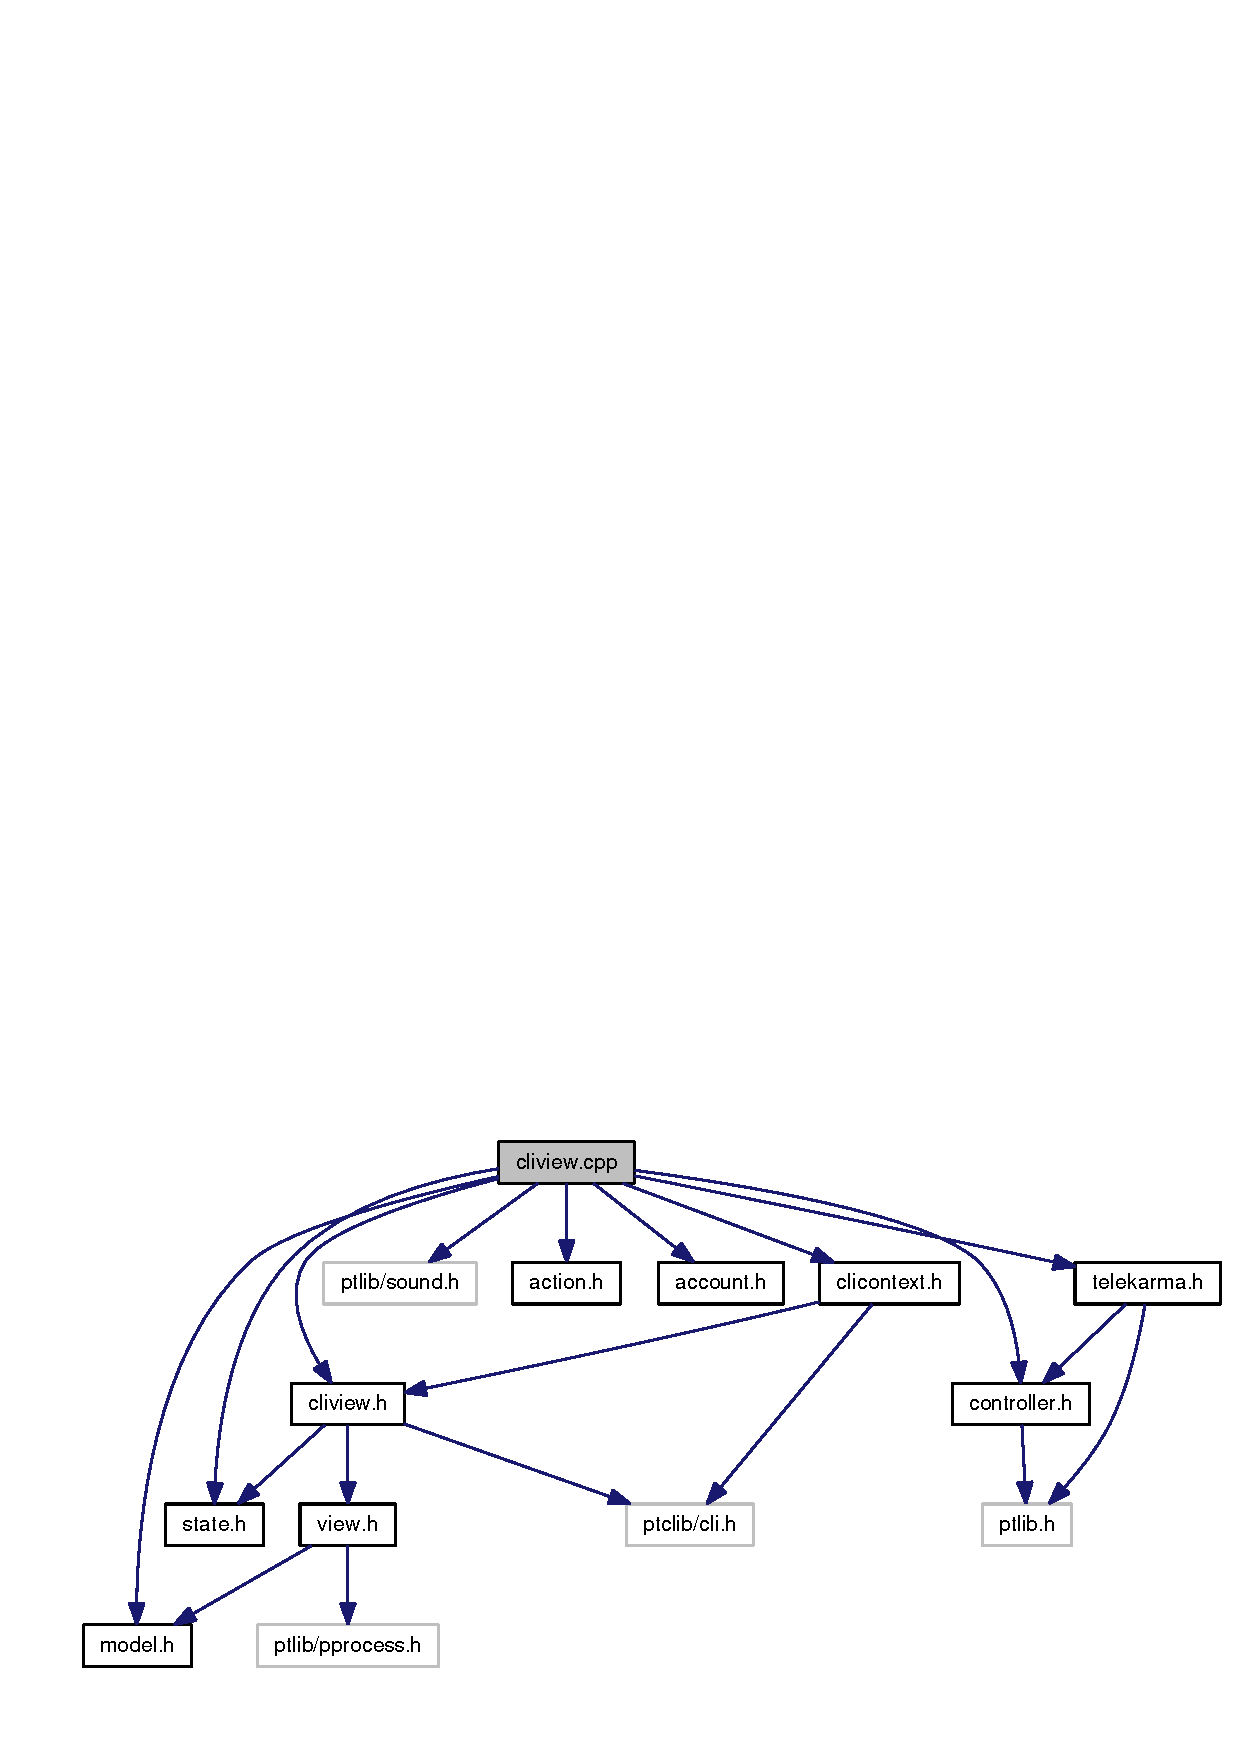
\includegraphics[width=295pt]{cliview_8cpp__incl}
\end{center}
\end{figure}

\hypertarget{cliview_8h}{
\section{cliview.h File Reference}
\label{cliview_8h}\index{cliview.h@{cliview.h}}
}
{\tt \#include $<$ptclib/cli.h$>$}\par
{\tt \#include \char`\"{}state.h\char`\"{}}\par
{\tt \#include \char`\"{}view.h\char`\"{}}\par


Include dependency graph for cliview.h:\nopagebreak
\begin{figure}[H]
\begin{center}
\leavevmode

\includegraphics[width=139pt]{cliview_8h__incl}
\end{center}
\end{figure}


This graph shows which files directly or indirectly include this file:\nopagebreak
\begin{figure}[H]
\begin{center}
\leavevmode

\includegraphics[width=127pt]{cliview_8h__dep__incl}
\end{center}
\end{figure}
\subsection*{Classes}
\begin{CompactItemize}
\item 
class \hyperlink{classCLIView}{CLIView}
\item 
class \textbf{CLIView::CLIView::InputHandler}
\begin{CompactList}\small\item\em Parent class for all of the \hyperlink{classCLIView}{CLIView} input handlers. \item\end{CompactList}\item 
class \textbf{CLIView::CLIView::STUNInputHandler}
\item 
class \textbf{CLIView::CLIView::RegistrarInputHandler}
\item 
class \textbf{CLIView::CLIView::UserInputHandler}
\item 
class \textbf{CLIView::CLIView::PasswordInputHandler}
\item 
class \textbf{CLIView::CLIView::DestInputHandler}
\item 
class \textbf{CLIView::CLIView::Command}
\end{CompactItemize}

\hypertarget{conf_8h}{
\section{conf.h File Reference}
\label{conf_8h}\index{conf.h@{conf.h}}
}
\subsection*{Defines}
\begin{CompactItemize}
\item 
\#define \hyperlink{conf_8h_25bf3a473b569af0e4123fd22a232518}{USE\_\-PRIMARY}~1
\begin{CompactList}\small\item\em \hyperlink{conf_8h}{conf.h} \item\end{CompactList}\item 
\#define \hyperlink{conf_8h_5af39456c6bdb1bece4788c90ff8d662}{USE\_\-ALT\_\-A}~1
\item 
\#define \hyperlink{conf_8h_0a1f4442d39b489ba271c93e3a3c0afd}{REGISTRAR}~\char`\"{}ekiga.net\char`\"{}
\item 
\#define \hyperlink{conf_8h_d07edadbb9bac1211ba8c0f5203aa33c}{STUN}~\char`\"{}stun.ekiga.net\char`\"{}
\item 
\#define \hyperlink{conf_8h_02776ef75ad1c9019695dfeabfada630}{ACCOUNT}~\char`\"{}\char`\"{}
\item 
\#define \hyperlink{conf_8h_9e8538fad4eee548302ad9f60e6d47ca}{PASSWORD}~\char`\"{}\char`\"{}
\item 
\#define \hyperlink{conf_8h_68d65624c5d231bf22e035bc07ed4d76}{DEST}~\char`\"{}sip:500@ekiga.net\char`\"{}
\end{CompactItemize}


\subsection{Define Documentation}
\hypertarget{conf_8h_02776ef75ad1c9019695dfeabfada630}{
\index{conf.h@{conf.h}!ACCOUNT@{ACCOUNT}}
\index{ACCOUNT@{ACCOUNT}!conf.h@{conf.h}}
\subsubsection[{ACCOUNT}]{\setlength{\rightskip}{0pt plus 5cm}\#define ACCOUNT~\char`\"{}\char`\"{}}}
\label{conf_8h_02776ef75ad1c9019695dfeabfada630}


\hypertarget{conf_8h_68d65624c5d231bf22e035bc07ed4d76}{
\index{conf.h@{conf.h}!DEST@{DEST}}
\index{DEST@{DEST}!conf.h@{conf.h}}
\subsubsection[{DEST}]{\setlength{\rightskip}{0pt plus 5cm}\#define DEST~\char`\"{}sip:500@ekiga.net\char`\"{}}}
\label{conf_8h_68d65624c5d231bf22e035bc07ed4d76}


\hypertarget{conf_8h_9e8538fad4eee548302ad9f60e6d47ca}{
\index{conf.h@{conf.h}!PASSWORD@{PASSWORD}}
\index{PASSWORD@{PASSWORD}!conf.h@{conf.h}}
\subsubsection[{PASSWORD}]{\setlength{\rightskip}{0pt plus 5cm}\#define PASSWORD~\char`\"{}\char`\"{}}}
\label{conf_8h_9e8538fad4eee548302ad9f60e6d47ca}


\hypertarget{conf_8h_0a1f4442d39b489ba271c93e3a3c0afd}{
\index{conf.h@{conf.h}!REGISTRAR@{REGISTRAR}}
\index{REGISTRAR@{REGISTRAR}!conf.h@{conf.h}}
\subsubsection[{REGISTRAR}]{\setlength{\rightskip}{0pt plus 5cm}\#define REGISTRAR~\char`\"{}ekiga.net\char`\"{}}}
\label{conf_8h_0a1f4442d39b489ba271c93e3a3c0afd}


\hypertarget{conf_8h_d07edadbb9bac1211ba8c0f5203aa33c}{
\index{conf.h@{conf.h}!STUN@{STUN}}
\index{STUN@{STUN}!conf.h@{conf.h}}
\subsubsection[{STUN}]{\setlength{\rightskip}{0pt plus 5cm}\#define STUN~\char`\"{}stun.ekiga.net\char`\"{}}}
\label{conf_8h_d07edadbb9bac1211ba8c0f5203aa33c}


\hypertarget{conf_8h_5af39456c6bdb1bece4788c90ff8d662}{
\index{conf.h@{conf.h}!USE\_\-ALT\_\-A@{USE\_\-ALT\_\-A}}
\index{USE\_\-ALT\_\-A@{USE\_\-ALT\_\-A}!conf.h@{conf.h}}
\subsubsection[{USE\_\-ALT\_\-A}]{\setlength{\rightskip}{0pt plus 5cm}\#define USE\_\-ALT\_\-A~1}}
\label{conf_8h_5af39456c6bdb1bece4788c90ff8d662}


\hypertarget{conf_8h_25bf3a473b569af0e4123fd22a232518}{
\index{conf.h@{conf.h}!USE\_\-PRIMARY@{USE\_\-PRIMARY}}
\index{USE\_\-PRIMARY@{USE\_\-PRIMARY}!conf.h@{conf.h}}
\subsubsection[{USE\_\-PRIMARY}]{\setlength{\rightskip}{0pt plus 5cm}\#define USE\_\-PRIMARY~1}}
\label{conf_8h_25bf3a473b569af0e4123fd22a232518}


\hyperlink{conf_8h}{conf.h} 

Convenience header for pre-specifying connection parameters for testing. 
\hypertarget{controller_8cpp}{
\section{controller.cpp File Reference}
\label{controller_8cpp}\index{controller.cpp@{controller.cpp}}
}
{\tt \#include \char`\"{}controller.h\char`\"{}}\par
{\tt \#include \char`\"{}model.h\char`\"{}}\par


Include dependency graph for controller.cpp:\nopagebreak
\begin{figure}[H]
\begin{center}
\leavevmode
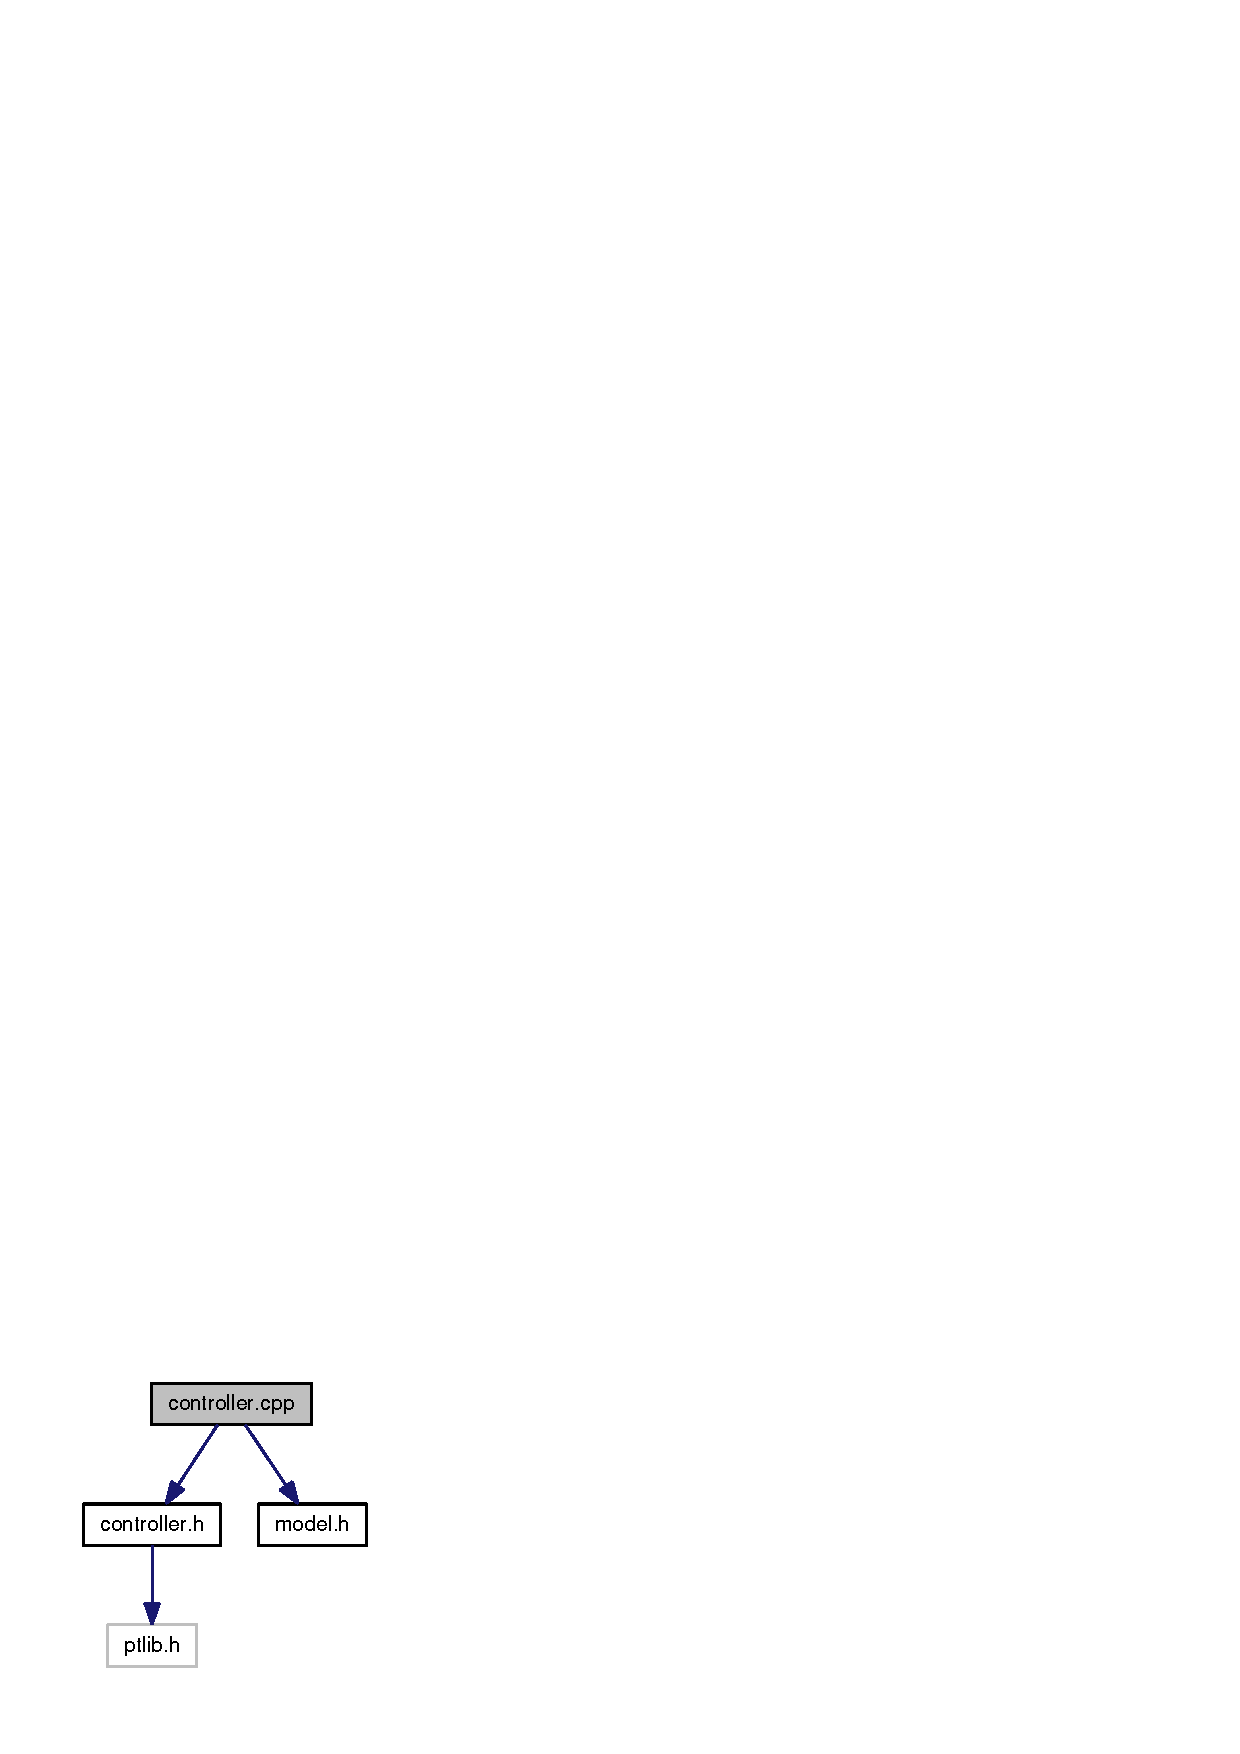
\includegraphics[width=90pt]{controller_8cpp__incl}
\end{center}
\end{figure}

\hypertarget{controller_8h}{
\section{controller.h File Reference}
\label{controller_8h}\index{controller.h@{controller.h}}
}
{\tt \#include $<$ptlib.h$>$}\par


Include dependency graph for controller.h:\nopagebreak
\begin{figure}[H]
\begin{center}
\leavevmode
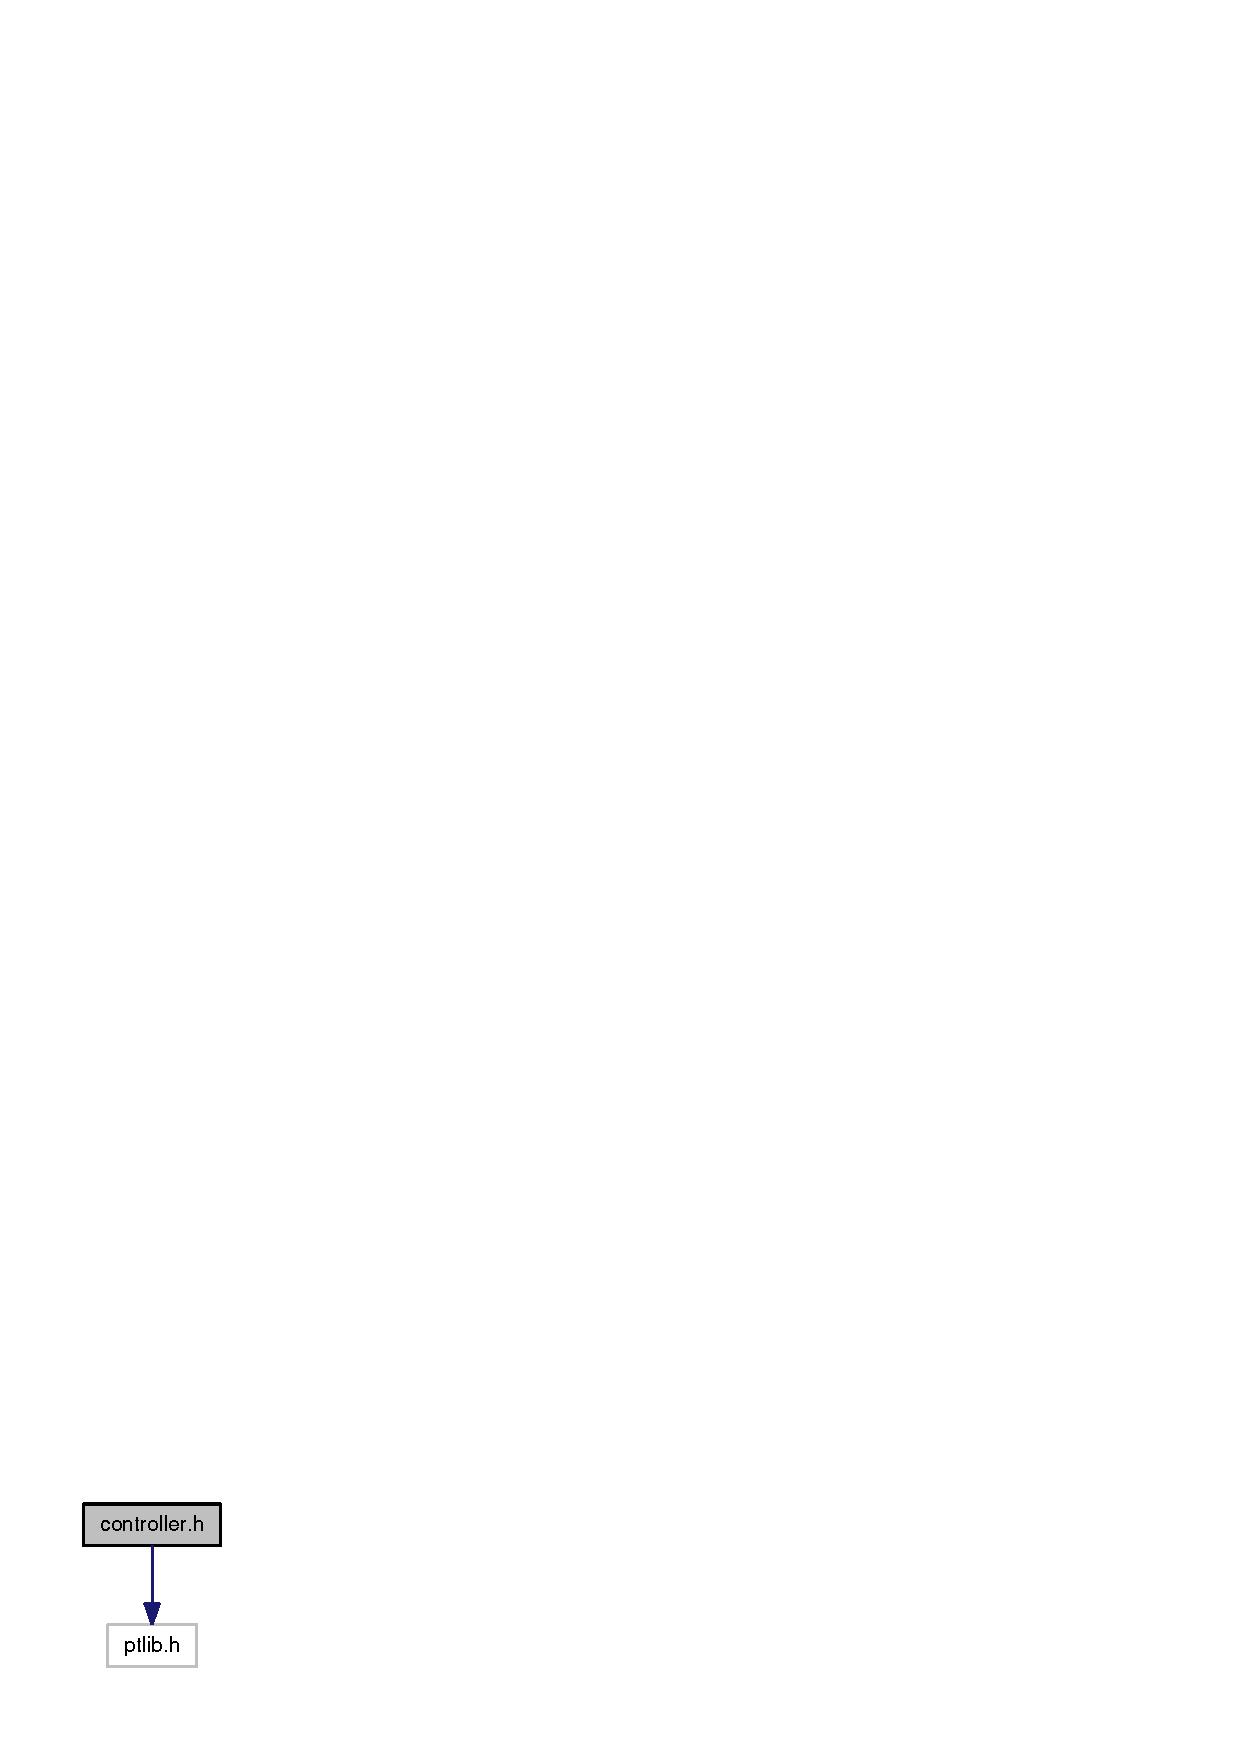
\includegraphics[width=55pt]{controller_8h__incl}
\end{center}
\end{figure}


This graph shows which files directly or indirectly include this file:\nopagebreak
\begin{figure}[H]
\begin{center}
\leavevmode
\includegraphics[width=138pt]{controller_8h__dep__incl}
\end{center}
\end{figure}
\subsection*{Classes}
\begin{CompactItemize}
\item 
class \hyperlink{classController}{Controller}
\end{CompactItemize}

\hypertarget{gui_8cpp}{
\section{gui.cpp File Reference}
\label{gui_8cpp}\index{gui.cpp@{gui.cpp}}
}
{\tt \#include $<$ptlib.h$>$}\par
{\tt \#include $<$ptlib/pprocess.h$>$}\par
{\tt \#include $<$wx/wx.h$>$}\par
{\tt \#include $<$sstream$>$}\par
{\tt \#include $<$cstring$>$}\par
{\tt \#include \char`\"{}state.h\char`\"{}}\par
{\tt \#include \char`\"{}action.h\char`\"{}}\par
{\tt \#include \char`\"{}model.h\char`\"{}}\par
{\tt \#include \char`\"{}view.h\char`\"{}}\par
{\tt \#include \char`\"{}telekarma.h\char`\"{}}\par
{\tt \#include \char`\"{}account.h\char`\"{}}\par
{\tt \#include $<$opal/mediafmt.h$>$}\par
{\tt \#include $<$ptlib/wxstring.h$>$}\par
{\tt \#include \char`\"{}gui.h\char`\"{}}\par


Include dependency graph for gui.cpp:\nopagebreak
\begin{figure}[H]
\begin{center}
\leavevmode
\includegraphics[width=420pt]{gui_8cpp__incl}
\end{center}
\end{figure}
\subsection*{Typedefs}
\begin{CompactItemize}
\item 
typedef stringstream \hyperlink{gui_8cpp_78812504638bb200e3c16b08979dcd02}{tstringstream}
\end{CompactItemize}
\subsection*{Functions}
\begin{CompactItemize}
\item 
PString \hyperlink{gui_8cpp_3f5b0ed75fc00f4732d4f9f5546c4009}{\_\-wxStr2Pstr} (const wxString \&str)
\item 
wxString \hyperlink{gui_8cpp_ab726773f3871ac02b70c6750b482acf}{\_\-Pstr2wxStr} (const PString \&str)
\end{CompactItemize}


\subsection{Typedef Documentation}
\hypertarget{gui_8cpp_78812504638bb200e3c16b08979dcd02}{
\index{gui.cpp@{gui.cpp}!tstringstream@{tstringstream}}
\index{tstringstream@{tstringstream}!gui.cpp@{gui.cpp}}
\subsubsection[{tstringstream}]{\setlength{\rightskip}{0pt plus 5cm}typedef stringstream {\bf tstringstream}}}
\label{gui_8cpp_78812504638bb200e3c16b08979dcd02}




\subsection{Function Documentation}
\hypertarget{gui_8cpp_ab726773f3871ac02b70c6750b482acf}{
\index{gui.cpp@{gui.cpp}!\_\-Pstr2wxStr@{\_\-Pstr2wxStr}}
\index{\_\-Pstr2wxStr@{\_\-Pstr2wxStr}!gui.cpp@{gui.cpp}}
\subsubsection[{\_\-Pstr2wxStr}]{\setlength{\rightskip}{0pt plus 5cm}wxString \_\-Pstr2wxStr (const PString \& {\em str})}}
\label{gui_8cpp_ab726773f3871ac02b70c6750b482acf}


\hypertarget{gui_8cpp_3f5b0ed75fc00f4732d4f9f5546c4009}{
\index{gui.cpp@{gui.cpp}!\_\-wxStr2Pstr@{\_\-wxStr2Pstr}}
\index{\_\-wxStr2Pstr@{\_\-wxStr2Pstr}!gui.cpp@{gui.cpp}}
\subsubsection[{\_\-wxStr2Pstr}]{\setlength{\rightskip}{0pt plus 5cm}PString \_\-wxStr2Pstr (const wxString \& {\em str})}}
\label{gui_8cpp_3f5b0ed75fc00f4732d4f9f5546c4009}



\hypertarget{gui_8h}{
\section{gui.h File Reference}
\label{gui_8h}\index{gui.h@{gui.h}}
}


This graph shows which files directly or indirectly include this file:\nopagebreak
\begin{figure}[H]
\begin{center}
\leavevmode
\includegraphics[width=46pt]{gui_8h__dep__incl}
\end{center}
\end{figure}
\subsection*{Classes}
\begin{CompactItemize}
\item 
class \hyperlink{classwxStateChangeEvent}{wxStateChangeEvent}
\item 
class \hyperlink{classwxRegisterDialogClosedEvent}{wxRegisterDialogClosedEvent}
\item 
class \hyperlink{classwxDialPadClosedEvent}{wxDialPadClosedEvent}
\item 
class \hyperlink{classTeleKarmaNG}{TeleKarmaNG}
\begin{CompactList}\small\item\em The main process. \item\end{CompactList}\item 
class \hyperlink{classMainFrame}{MainFrame}
\begin{CompactList}\small\item\em The main window. \item\end{CompactList}\item 
class \hyperlink{classRegisterDialog}{RegisterDialog}
\begin{CompactList}\small\item\em Modal registration dialog box. \item\end{CompactList}\item 
class \hyperlink{classDialPad}{DialPad}
\begin{CompactList}\small\item\em Dial pad for touch tone transmission. \item\end{CompactList}\item 
class \hyperlink{classStateHelper}{StateHelper}
\begin{CompactList}\small\item\em Utilities for mapping state id and other state-derived data to meaningful semantics and messages. \item\end{CompactList}\end{CompactItemize}
\subsection*{Defines}
\begin{CompactItemize}
\item 
\#define \hyperlink{gui_8h_2fd81ded1b6a151f629441182c358d5b}{PRODUCT\_\-NAME}~\char`\"{}TeleKarma NG\char`\"{}
\item 
\#define \hyperlink{gui_8h_1c6d5de492ac61ad29aec7aa9a436bbf}{VERSION}~\char`\"{}0.1.002\char`\"{}
\item 
\#define \hyperlink{gui_8h_0bff94a0d5c29e72fd5459933019db7d}{COPYRIGHT\_\-HOLDER}~\char`\"{}Thomas Stellard, Michael Volk, Nikhil Tripathi and Peter Batzel\char`\"{}
\item 
\#define \hyperlink{gui_8h_ceec47906f5ee7badf2b8398941cd016}{EVT\_\-STATE}(id, fn)
\item 
\#define \hyperlink{gui_8h_380ef9893c751b2aa536614bb06667bc}{EVT\_\-REGISTER\_\-DIALOG\_\-CLOSED}(id, fn)
\item 
\#define \hyperlink{gui_8h_a7a14de65321aae213fa1bf6296d4da7}{EVT\_\-DIAL\_\-PAD\_\-CLOSED}(id, fn)
\end{CompactItemize}
\subsection*{Typedefs}
\begin{CompactItemize}
\item 
typedef void(wxEvtHandler::$\ast$ \hyperlink{gui_8h_2bd601b6476eb4a30ff58a621ac77dbc}{wxStateChangeEventFunction} )(\hyperlink{classwxStateChangeEvent}{wxStateChangeEvent} \&)
\item 
typedef void(wxEvtHandler::$\ast$ \hyperlink{gui_8h_6f5c9031b4afd4c6c1b837beacf5909d}{wxRegisterDialogClosedEventFunction} )(\hyperlink{classwxRegisterDialogClosedEvent}{wxRegisterDialogClosedEvent} \&)
\item 
typedef void(wxEvtHandler::$\ast$ \hyperlink{gui_8h_f0e8a28d7b4e8891661fef371286e7e7}{wxDialPadClosedEventFunction} )(\hyperlink{classwxDialPadClosedEvent}{wxDialPadClosedEvent} \&)
\end{CompactItemize}
\subsection*{Enumerations}
\begin{CompactItemize}
\item 
enum \{ \par
\hyperlink{gui_8h_06fc87d81c62e9abb8790b6e5713c55b982306e68d56775c32654fc2b29cf3bf}{evRegister} =  1, 
\hyperlink{gui_8h_06fc87d81c62e9abb8790b6e5713c55be6e396e0cbe1e9ef1ecc7bcc5a68fb09}{evAccounts} =  2, 
\hyperlink{gui_8h_06fc87d81c62e9abb8790b6e5713c55bffd9f6d137fb7c87e4258ffb36f8ddc2}{evContacts} =  3, 
\hyperlink{gui_8h_06fc87d81c62e9abb8790b6e5713c55b154b51d77fad1182dd4b595d90b1595c}{evDial} =  4, 
\par
\hyperlink{gui_8h_06fc87d81c62e9abb8790b6e5713c55b89af2bef3ffc25bb3b378c8e0375c064}{evDialPad} =  5, 
\hyperlink{gui_8h_06fc87d81c62e9abb8790b6e5713c55bb57fc4769eade43752b65c0235508e19}{evHold} =  6, 
\hyperlink{gui_8h_06fc87d81c62e9abb8790b6e5713c55b64add398a0c4ca5e33e2779d157c7115}{evAutoHold} =  7, 
\hyperlink{gui_8h_06fc87d81c62e9abb8790b6e5713c55b7becd2da33fc4be1963ecb16d9a8eea4}{evRetrieve} =  8, 
\par
\hyperlink{gui_8h_06fc87d81c62e9abb8790b6e5713c55beefa3c83f7e7731bb43e8a0fbd1d14ae}{evHangUp} =  9
 \}
\begin{CompactList}\small\item\em Events the GUI can generate. \item\end{CompactList}\item 
enum \{ \par
\hyperlink{gui_8h_df764cbdea00d65edcd07bb9953ad2b71e3411649f99cf860485c2f9372e299b}{tkID\_\-REGISTER\_\-BTN} =  101, 
\hyperlink{gui_8h_df764cbdea00d65edcd07bb9953ad2b7b101a4f812671a45f9d2bcf39f2eea0d}{tkID\_\-DIALPAD\_\-ONE} =  102, 
\hyperlink{gui_8h_df764cbdea00d65edcd07bb9953ad2b7dcbbcaf1d0b7fd54d58c3610e9c47d52}{tkID\_\-DIALPAD\_\-TWO} =  103, 
\hyperlink{gui_8h_df764cbdea00d65edcd07bb9953ad2b7d7b2d45b4b4f6a4cfd2cab5c531710e0}{tkID\_\-DIALPAD\_\-THREE} =  104, 
\par
\hyperlink{gui_8h_df764cbdea00d65edcd07bb9953ad2b76997077e0775572ccfa39aec17f1ccf5}{tkID\_\-DIALPAD\_\-FOUR} =  105, 
\hyperlink{gui_8h_df764cbdea00d65edcd07bb9953ad2b7908c3c091bb10972b18757b8893fd704}{tkID\_\-DIALPAD\_\-FIVE} =  106, 
\hyperlink{gui_8h_df764cbdea00d65edcd07bb9953ad2b7426ca3c541712a94602f64aa15f384df}{tkID\_\-DIALPAD\_\-SIX} =  107, 
\hyperlink{gui_8h_df764cbdea00d65edcd07bb9953ad2b7149a567b69b43f9549b2fd8d00df0136}{tkID\_\-DIALPAD\_\-SEVEN} =  108, 
\par
\hyperlink{gui_8h_df764cbdea00d65edcd07bb9953ad2b744b3c73d711463dcbf1cb265b0a68285}{tkID\_\-DIALPAD\_\-EIGHT} =  109, 
\hyperlink{gui_8h_df764cbdea00d65edcd07bb9953ad2b780098dcdc781de83212015e9fea0f08c}{tkID\_\-DIALPAD\_\-NINE} =  110, 
\hyperlink{gui_8h_df764cbdea00d65edcd07bb9953ad2b7febd119a40367a83c6416b52070d03bf}{tkID\_\-DIALPAD\_\-ZERO} =  111, 
\hyperlink{gui_8h_df764cbdea00d65edcd07bb9953ad2b7eea5f1d8b453a2e6272e8eb7a4146f15}{tkID\_\-DIALPAD\_\-POUND} =  112, 
\par
\hyperlink{gui_8h_df764cbdea00d65edcd07bb9953ad2b7a79efe614e5a9d29ec4272e46261c815}{tkID\_\-DIALPAD\_\-STAR} =  113, 
\hyperlink{gui_8h_df764cbdea00d65edcd07bb9953ad2b7a85ecc98e1bd7d40fa8f1bc90c71cbd9}{tkID\_\-DIAL\_\-BTN} =  114, 
\hyperlink{gui_8h_df764cbdea00d65edcd07bb9953ad2b768f2e3c9943d51a7f4a6febbc44639a8}{tkID\_\-DESTINATION} =  115
 \}
\begin{CompactList}\small\item\em Unique widget identifiers. \item\end{CompactList}\end{CompactItemize}


\subsection{Define Documentation}
\hypertarget{gui_8h_0bff94a0d5c29e72fd5459933019db7d}{
\index{gui.h@{gui.h}!COPYRIGHT\_\-HOLDER@{COPYRIGHT\_\-HOLDER}}
\index{COPYRIGHT\_\-HOLDER@{COPYRIGHT\_\-HOLDER}!gui.h@{gui.h}}
\subsubsection[{COPYRIGHT\_\-HOLDER}]{\setlength{\rightskip}{0pt plus 5cm}\#define COPYRIGHT\_\-HOLDER~\char`\"{}Thomas Stellard, Michael Volk, Nikhil Tripathi and Peter Batzel\char`\"{}}}
\label{gui_8h_0bff94a0d5c29e72fd5459933019db7d}


\hypertarget{gui_8h_a7a14de65321aae213fa1bf6296d4da7}{
\index{gui.h@{gui.h}!EVT\_\-DIAL\_\-PAD\_\-CLOSED@{EVT\_\-DIAL\_\-PAD\_\-CLOSED}}
\index{EVT\_\-DIAL\_\-PAD\_\-CLOSED@{EVT\_\-DIAL\_\-PAD\_\-CLOSED}!gui.h@{gui.h}}
\subsubsection[{EVT\_\-DIAL\_\-PAD\_\-CLOSED}]{\setlength{\rightskip}{0pt plus 5cm}\#define EVT\_\-DIAL\_\-PAD\_\-CLOSED(id, \/  fn)}}
\label{gui_8h_a7a14de65321aae213fa1bf6296d4da7}


\textbf{Value:}

\begin{Code}\begin{verbatim}DECLARE_EVENT_TABLE_ENTRY( wxEVT_DIAL_PAD_CLOSED, id, -1, \
    (wxObjectEventFunction) (wxEventFunction) (wxCommandEventFunction) (wxNotifyEventFunction) \
    wxStaticCastEvent( wxDialPadClosedEventFunction, & fn ), (wxObject *) NULL ),
\end{verbatim}
\end{Code}
\hypertarget{gui_8h_380ef9893c751b2aa536614bb06667bc}{
\index{gui.h@{gui.h}!EVT\_\-REGISTER\_\-DIALOG\_\-CLOSED@{EVT\_\-REGISTER\_\-DIALOG\_\-CLOSED}}
\index{EVT\_\-REGISTER\_\-DIALOG\_\-CLOSED@{EVT\_\-REGISTER\_\-DIALOG\_\-CLOSED}!gui.h@{gui.h}}
\subsubsection[{EVT\_\-REGISTER\_\-DIALOG\_\-CLOSED}]{\setlength{\rightskip}{0pt plus 5cm}\#define EVT\_\-REGISTER\_\-DIALOG\_\-CLOSED(id, \/  fn)}}
\label{gui_8h_380ef9893c751b2aa536614bb06667bc}


\textbf{Value:}

\begin{Code}\begin{verbatim}DECLARE_EVENT_TABLE_ENTRY( wxEVT_REGISTER_DIALOG_CLOSED, id, -1, \
    (wxObjectEventFunction) (wxEventFunction) (wxCommandEventFunction) (wxNotifyEventFunction) \
    wxStaticCastEvent( wxRegisterDialogClosedEventFunction, & fn ), (wxObject *) NULL ),
\end{verbatim}
\end{Code}
\hypertarget{gui_8h_ceec47906f5ee7badf2b8398941cd016}{
\index{gui.h@{gui.h}!EVT\_\-STATE@{EVT\_\-STATE}}
\index{EVT\_\-STATE@{EVT\_\-STATE}!gui.h@{gui.h}}
\subsubsection[{EVT\_\-STATE}]{\setlength{\rightskip}{0pt plus 5cm}\#define EVT\_\-STATE(id, \/  fn)}}
\label{gui_8h_ceec47906f5ee7badf2b8398941cd016}


\textbf{Value:}

\begin{Code}\begin{verbatim}DECLARE_EVENT_TABLE_ENTRY( wxEVT_STATE_CHANGE, id, -1, \
    (wxObjectEventFunction) (wxEventFunction) (wxCommandEventFunction) (wxNotifyEventFunction) \
    wxStaticCastEvent( wxStateChangeEventFunction, & fn ), (wxObject *) NULL ),
\end{verbatim}
\end{Code}
\hypertarget{gui_8h_2fd81ded1b6a151f629441182c358d5b}{
\index{gui.h@{gui.h}!PRODUCT\_\-NAME@{PRODUCT\_\-NAME}}
\index{PRODUCT\_\-NAME@{PRODUCT\_\-NAME}!gui.h@{gui.h}}
\subsubsection[{PRODUCT\_\-NAME}]{\setlength{\rightskip}{0pt plus 5cm}\#define PRODUCT\_\-NAME~\char`\"{}TeleKarma NG\char`\"{}}}
\label{gui_8h_2fd81ded1b6a151f629441182c358d5b}


\hypertarget{gui_8h_1c6d5de492ac61ad29aec7aa9a436bbf}{
\index{gui.h@{gui.h}!VERSION@{VERSION}}
\index{VERSION@{VERSION}!gui.h@{gui.h}}
\subsubsection[{VERSION}]{\setlength{\rightskip}{0pt plus 5cm}\#define VERSION~\char`\"{}0.1.002\char`\"{}}}
\label{gui_8h_1c6d5de492ac61ad29aec7aa9a436bbf}




\subsection{Typedef Documentation}
\hypertarget{gui_8h_f0e8a28d7b4e8891661fef371286e7e7}{
\index{gui.h@{gui.h}!wxDialPadClosedEventFunction@{wxDialPadClosedEventFunction}}
\index{wxDialPadClosedEventFunction@{wxDialPadClosedEventFunction}!gui.h@{gui.h}}
\subsubsection[{wxDialPadClosedEventFunction}]{\setlength{\rightskip}{0pt plus 5cm}typedef void(wxEvtHandler::$\ast$ {\bf wxDialPadClosedEventFunction})({\bf wxDialPadClosedEvent} \&)}}
\label{gui_8h_f0e8a28d7b4e8891661fef371286e7e7}


\hypertarget{gui_8h_6f5c9031b4afd4c6c1b837beacf5909d}{
\index{gui.h@{gui.h}!wxRegisterDialogClosedEventFunction@{wxRegisterDialogClosedEventFunction}}
\index{wxRegisterDialogClosedEventFunction@{wxRegisterDialogClosedEventFunction}!gui.h@{gui.h}}
\subsubsection[{wxRegisterDialogClosedEventFunction}]{\setlength{\rightskip}{0pt plus 5cm}typedef void(wxEvtHandler::$\ast$ {\bf wxRegisterDialogClosedEventFunction})({\bf wxRegisterDialogClosedEvent} \&)}}
\label{gui_8h_6f5c9031b4afd4c6c1b837beacf5909d}


\hypertarget{gui_8h_2bd601b6476eb4a30ff58a621ac77dbc}{
\index{gui.h@{gui.h}!wxStateChangeEventFunction@{wxStateChangeEventFunction}}
\index{wxStateChangeEventFunction@{wxStateChangeEventFunction}!gui.h@{gui.h}}
\subsubsection[{wxStateChangeEventFunction}]{\setlength{\rightskip}{0pt plus 5cm}typedef void(wxEvtHandler::$\ast$ {\bf wxStateChangeEventFunction})({\bf wxStateChangeEvent} \&)}}
\label{gui_8h_2bd601b6476eb4a30ff58a621ac77dbc}




\subsection{Enumeration Type Documentation}
\hypertarget{gui_8h_06fc87d81c62e9abb8790b6e5713c55b}{
\subsubsection[{"@0}]{\setlength{\rightskip}{0pt plus 5cm}anonymous enum}}
\label{gui_8h_06fc87d81c62e9abb8790b6e5713c55b}


Events the GUI can generate. 

\begin{Desc}
\item[Enumerator: ]\par
\begin{description}
\index{evRegister@{evRegister}!gui.h@{gui.h}}\index{gui.h@{gui.h}!evRegister@{evRegister}}\item[{\em 
\hypertarget{gui_8h_06fc87d81c62e9abb8790b6e5713c55b982306e68d56775c32654fc2b29cf3bf}{
evRegister}
\label{gui_8h_06fc87d81c62e9abb8790b6e5713c55b982306e68d56775c32654fc2b29cf3bf}
}]File -$>$ Register. 

.. \index{evAccounts@{evAccounts}!gui.h@{gui.h}}\index{gui.h@{gui.h}!evAccounts@{evAccounts}}\item[{\em 
\hypertarget{gui_8h_06fc87d81c62e9abb8790b6e5713c55be6e396e0cbe1e9ef1ecc7bcc5a68fb09}{
evAccounts}
\label{gui_8h_06fc87d81c62e9abb8790b6e5713c55be6e396e0cbe1e9ef1ecc7bcc5a68fb09}
}]Edit -$>$ Accounts. 

.. \index{evContacts@{evContacts}!gui.h@{gui.h}}\index{gui.h@{gui.h}!evContacts@{evContacts}}\item[{\em 
\hypertarget{gui_8h_06fc87d81c62e9abb8790b6e5713c55bffd9f6d137fb7c87e4258ffb36f8ddc2}{
evContacts}
\label{gui_8h_06fc87d81c62e9abb8790b6e5713c55bffd9f6d137fb7c87e4258ffb36f8ddc2}
}]Edit -$>$ Contacts. 

.. \index{evDial@{evDial}!gui.h@{gui.h}}\index{gui.h@{gui.h}!evDial@{evDial}}\item[{\em 
\hypertarget{gui_8h_06fc87d81c62e9abb8790b6e5713c55b154b51d77fad1182dd4b595d90b1595c}{
evDial}
\label{gui_8h_06fc87d81c62e9abb8790b6e5713c55b154b51d77fad1182dd4b595d90b1595c}
}]Call -$>$ Dial. \index{evDialPad@{evDialPad}!gui.h@{gui.h}}\index{gui.h@{gui.h}!evDialPad@{evDialPad}}\item[{\em 
\hypertarget{gui_8h_06fc87d81c62e9abb8790b6e5713c55b89af2bef3ffc25bb3b378c8e0375c064}{
evDialPad}
\label{gui_8h_06fc87d81c62e9abb8790b6e5713c55b89af2bef3ffc25bb3b378c8e0375c064}
}]Call -$>$ Touch Tones. 

.. \index{evHold@{evHold}!gui.h@{gui.h}}\index{gui.h@{gui.h}!evHold@{evHold}}\item[{\em 
\hypertarget{gui_8h_06fc87d81c62e9abb8790b6e5713c55bb57fc4769eade43752b65c0235508e19}{
evHold}
\label{gui_8h_06fc87d81c62e9abb8790b6e5713c55bb57fc4769eade43752b65c0235508e19}
}]Call -$>$ Hold. \index{evAutoHold@{evAutoHold}!gui.h@{gui.h}}\index{gui.h@{gui.h}!evAutoHold@{evAutoHold}}\item[{\em 
\hypertarget{gui_8h_06fc87d81c62e9abb8790b6e5713c55b64add398a0c4ca5e33e2779d157c7115}{
evAutoHold}
\label{gui_8h_06fc87d81c62e9abb8790b6e5713c55b64add398a0c4ca5e33e2779d157c7115}
}]Call -$>$ AutoHold. \index{evRetrieve@{evRetrieve}!gui.h@{gui.h}}\index{gui.h@{gui.h}!evRetrieve@{evRetrieve}}\item[{\em 
\hypertarget{gui_8h_06fc87d81c62e9abb8790b6e5713c55b7becd2da33fc4be1963ecb16d9a8eea4}{
evRetrieve}
\label{gui_8h_06fc87d81c62e9abb8790b6e5713c55b7becd2da33fc4be1963ecb16d9a8eea4}
}]Call -$>$ Retrieve. \index{evHangUp@{evHangUp}!gui.h@{gui.h}}\index{gui.h@{gui.h}!evHangUp@{evHangUp}}\item[{\em 
\hypertarget{gui_8h_06fc87d81c62e9abb8790b6e5713c55beefa3c83f7e7731bb43e8a0fbd1d14ae}{
evHangUp}
\label{gui_8h_06fc87d81c62e9abb8790b6e5713c55beefa3c83f7e7731bb43e8a0fbd1d14ae}
}]Call -$>$ Hang Up. \end{description}
\end{Desc}

\hypertarget{gui_8h_df764cbdea00d65edcd07bb9953ad2b7}{
\subsubsection[{"@1}]{\setlength{\rightskip}{0pt plus 5cm}anonymous enum}}
\label{gui_8h_df764cbdea00d65edcd07bb9953ad2b7}


Unique widget identifiers. 

\begin{Desc}
\item[Enumerator: ]\par
\begin{description}
\index{tkID\_\-REGISTER\_\-BTN@{tkID\_\-REGISTER\_\-BTN}!gui.h@{gui.h}}\index{gui.h@{gui.h}!tkID\_\-REGISTER\_\-BTN@{tkID\_\-REGISTER\_\-BTN}}\item[{\em 
\hypertarget{gui_8h_df764cbdea00d65edcd07bb9953ad2b71e3411649f99cf860485c2f9372e299b}{
tkID\_\-REGISTER\_\-BTN}
\label{gui_8h_df764cbdea00d65edcd07bb9953ad2b71e3411649f99cf860485c2f9372e299b}
}]Register button on register dialog. 

\index{tkID\_\-DIALPAD\_\-ONE@{tkID\_\-DIALPAD\_\-ONE}!gui.h@{gui.h}}\index{gui.h@{gui.h}!tkID\_\-DIALPAD\_\-ONE@{tkID\_\-DIALPAD\_\-ONE}}\item[{\em 
\hypertarget{gui_8h_df764cbdea00d65edcd07bb9953ad2b7b101a4f812671a45f9d2bcf39f2eea0d}{
tkID\_\-DIALPAD\_\-ONE}
\label{gui_8h_df764cbdea00d65edcd07bb9953ad2b7b101a4f812671a45f9d2bcf39f2eea0d}
}]Dial pad button. 

\index{tkID\_\-DIALPAD\_\-TWO@{tkID\_\-DIALPAD\_\-TWO}!gui.h@{gui.h}}\index{gui.h@{gui.h}!tkID\_\-DIALPAD\_\-TWO@{tkID\_\-DIALPAD\_\-TWO}}\item[{\em 
\hypertarget{gui_8h_df764cbdea00d65edcd07bb9953ad2b7dcbbcaf1d0b7fd54d58c3610e9c47d52}{
tkID\_\-DIALPAD\_\-TWO}
\label{gui_8h_df764cbdea00d65edcd07bb9953ad2b7dcbbcaf1d0b7fd54d58c3610e9c47d52}
}]Dial pad button. 

\index{tkID\_\-DIALPAD\_\-THREE@{tkID\_\-DIALPAD\_\-THREE}!gui.h@{gui.h}}\index{gui.h@{gui.h}!tkID\_\-DIALPAD\_\-THREE@{tkID\_\-DIALPAD\_\-THREE}}\item[{\em 
\hypertarget{gui_8h_df764cbdea00d65edcd07bb9953ad2b7d7b2d45b4b4f6a4cfd2cab5c531710e0}{
tkID\_\-DIALPAD\_\-THREE}
\label{gui_8h_df764cbdea00d65edcd07bb9953ad2b7d7b2d45b4b4f6a4cfd2cab5c531710e0}
}]Dial pad button. 

\index{tkID\_\-DIALPAD\_\-FOUR@{tkID\_\-DIALPAD\_\-FOUR}!gui.h@{gui.h}}\index{gui.h@{gui.h}!tkID\_\-DIALPAD\_\-FOUR@{tkID\_\-DIALPAD\_\-FOUR}}\item[{\em 
\hypertarget{gui_8h_df764cbdea00d65edcd07bb9953ad2b76997077e0775572ccfa39aec17f1ccf5}{
tkID\_\-DIALPAD\_\-FOUR}
\label{gui_8h_df764cbdea00d65edcd07bb9953ad2b76997077e0775572ccfa39aec17f1ccf5}
}]Dial pad button. 

\index{tkID\_\-DIALPAD\_\-FIVE@{tkID\_\-DIALPAD\_\-FIVE}!gui.h@{gui.h}}\index{gui.h@{gui.h}!tkID\_\-DIALPAD\_\-FIVE@{tkID\_\-DIALPAD\_\-FIVE}}\item[{\em 
\hypertarget{gui_8h_df764cbdea00d65edcd07bb9953ad2b7908c3c091bb10972b18757b8893fd704}{
tkID\_\-DIALPAD\_\-FIVE}
\label{gui_8h_df764cbdea00d65edcd07bb9953ad2b7908c3c091bb10972b18757b8893fd704}
}]Dial pad button. 

\index{tkID\_\-DIALPAD\_\-SIX@{tkID\_\-DIALPAD\_\-SIX}!gui.h@{gui.h}}\index{gui.h@{gui.h}!tkID\_\-DIALPAD\_\-SIX@{tkID\_\-DIALPAD\_\-SIX}}\item[{\em 
\hypertarget{gui_8h_df764cbdea00d65edcd07bb9953ad2b7426ca3c541712a94602f64aa15f384df}{
tkID\_\-DIALPAD\_\-SIX}
\label{gui_8h_df764cbdea00d65edcd07bb9953ad2b7426ca3c541712a94602f64aa15f384df}
}]Dial pad button. 

\index{tkID\_\-DIALPAD\_\-SEVEN@{tkID\_\-DIALPAD\_\-SEVEN}!gui.h@{gui.h}}\index{gui.h@{gui.h}!tkID\_\-DIALPAD\_\-SEVEN@{tkID\_\-DIALPAD\_\-SEVEN}}\item[{\em 
\hypertarget{gui_8h_df764cbdea00d65edcd07bb9953ad2b7149a567b69b43f9549b2fd8d00df0136}{
tkID\_\-DIALPAD\_\-SEVEN}
\label{gui_8h_df764cbdea00d65edcd07bb9953ad2b7149a567b69b43f9549b2fd8d00df0136}
}]Dial pad button. 

\index{tkID\_\-DIALPAD\_\-EIGHT@{tkID\_\-DIALPAD\_\-EIGHT}!gui.h@{gui.h}}\index{gui.h@{gui.h}!tkID\_\-DIALPAD\_\-EIGHT@{tkID\_\-DIALPAD\_\-EIGHT}}\item[{\em 
\hypertarget{gui_8h_df764cbdea00d65edcd07bb9953ad2b744b3c73d711463dcbf1cb265b0a68285}{
tkID\_\-DIALPAD\_\-EIGHT}
\label{gui_8h_df764cbdea00d65edcd07bb9953ad2b744b3c73d711463dcbf1cb265b0a68285}
}]Dial pad button. 

\index{tkID\_\-DIALPAD\_\-NINE@{tkID\_\-DIALPAD\_\-NINE}!gui.h@{gui.h}}\index{gui.h@{gui.h}!tkID\_\-DIALPAD\_\-NINE@{tkID\_\-DIALPAD\_\-NINE}}\item[{\em 
\hypertarget{gui_8h_df764cbdea00d65edcd07bb9953ad2b780098dcdc781de83212015e9fea0f08c}{
tkID\_\-DIALPAD\_\-NINE}
\label{gui_8h_df764cbdea00d65edcd07bb9953ad2b780098dcdc781de83212015e9fea0f08c}
}]Dial pad button. 

\index{tkID\_\-DIALPAD\_\-ZERO@{tkID\_\-DIALPAD\_\-ZERO}!gui.h@{gui.h}}\index{gui.h@{gui.h}!tkID\_\-DIALPAD\_\-ZERO@{tkID\_\-DIALPAD\_\-ZERO}}\item[{\em 
\hypertarget{gui_8h_df764cbdea00d65edcd07bb9953ad2b7febd119a40367a83c6416b52070d03bf}{
tkID\_\-DIALPAD\_\-ZERO}
\label{gui_8h_df764cbdea00d65edcd07bb9953ad2b7febd119a40367a83c6416b52070d03bf}
}]Dial pad button. 

\index{tkID\_\-DIALPAD\_\-POUND@{tkID\_\-DIALPAD\_\-POUND}!gui.h@{gui.h}}\index{gui.h@{gui.h}!tkID\_\-DIALPAD\_\-POUND@{tkID\_\-DIALPAD\_\-POUND}}\item[{\em 
\hypertarget{gui_8h_df764cbdea00d65edcd07bb9953ad2b7eea5f1d8b453a2e6272e8eb7a4146f15}{
tkID\_\-DIALPAD\_\-POUND}
\label{gui_8h_df764cbdea00d65edcd07bb9953ad2b7eea5f1d8b453a2e6272e8eb7a4146f15}
}]Dial pad button. 

\index{tkID\_\-DIALPAD\_\-STAR@{tkID\_\-DIALPAD\_\-STAR}!gui.h@{gui.h}}\index{gui.h@{gui.h}!tkID\_\-DIALPAD\_\-STAR@{tkID\_\-DIALPAD\_\-STAR}}\item[{\em 
\hypertarget{gui_8h_df764cbdea00d65edcd07bb9953ad2b7a79efe614e5a9d29ec4272e46261c815}{
tkID\_\-DIALPAD\_\-STAR}
\label{gui_8h_df764cbdea00d65edcd07bb9953ad2b7a79efe614e5a9d29ec4272e46261c815}
}]Dial pad button. 

\index{tkID\_\-DIAL\_\-BTN@{tkID\_\-DIAL\_\-BTN}!gui.h@{gui.h}}\index{gui.h@{gui.h}!tkID\_\-DIAL\_\-BTN@{tkID\_\-DIAL\_\-BTN}}\item[{\em 
\hypertarget{gui_8h_df764cbdea00d65edcd07bb9953ad2b7a85ecc98e1bd7d40fa8f1bc90c71cbd9}{
tkID\_\-DIAL\_\-BTN}
\label{gui_8h_df764cbdea00d65edcd07bb9953ad2b7a85ecc98e1bd7d40fa8f1bc90c71cbd9}
}]Dial/Hang Up button in main frame. 

\index{tkID\_\-DESTINATION@{tkID\_\-DESTINATION}!gui.h@{gui.h}}\index{gui.h@{gui.h}!tkID\_\-DESTINATION@{tkID\_\-DESTINATION}}\item[{\em 
\hypertarget{gui_8h_df764cbdea00d65edcd07bb9953ad2b768f2e3c9943d51a7f4a6febbc44639a8}{
tkID\_\-DESTINATION}
\label{gui_8h_df764cbdea00d65edcd07bb9953ad2b768f2e3c9943d51a7f4a6febbc44639a8}
}]SIP phone number text box. \end{description}
\end{Desc}


\hypertarget{main_8cpp}{
\section{main.cpp File Reference}
\label{main_8cpp}\index{main.cpp@{main.cpp}}
}
{\tt \#include $<$ptlib.h$>$}\par
{\tt \#include \char`\"{}cliview.h\char`\"{}}\par


Include dependency graph for main.cpp:\nopagebreak
\begin{figure}[H]
\begin{center}
\leavevmode
\includegraphics[width=139pt]{main_8cpp__incl}
\end{center}
\end{figure}
\subsection*{Functions}
\begin{CompactItemize}
\item 
\hyperlink{main_8cpp_7fdb2896b3ae3bf4fc9de267ce4999cd}{PCREATE\_\-PROCESS} (\hyperlink{classCLIView}{CLIView})
\begin{CompactList}\small\item\em The PCREATE\_\-PROCESS macro. \item\end{CompactList}\end{CompactItemize}


\subsection{Function Documentation}
\hypertarget{main_8cpp_7fdb2896b3ae3bf4fc9de267ce4999cd}{
\index{main.cpp@{main.cpp}!PCREATE\_\-PROCESS@{PCREATE\_\-PROCESS}}
\index{PCREATE\_\-PROCESS@{PCREATE\_\-PROCESS}!main.cpp@{main.cpp}}
\subsubsection[{PCREATE\_\-PROCESS}]{\setlength{\rightskip}{0pt plus 5cm}PCREATE\_\-PROCESS ({\bf CLIView})}}
\label{main_8cpp_7fdb2896b3ae3bf4fc9de267ce4999cd}


The PCREATE\_\-PROCESS macro. 

.. 1. Defines the main() function. 2. Creates an instance of \hyperlink{classTeleKarma}{TeleKarma}. 3. Calls instance-$>$PreInitialise() which is inherited from PProcess. 4. Calls instance-$>$InternalMain() which is inherited from PProcess. 5. instance-$>$InternalMain() calls instance-$>$Main() which must be defined in \hyperlink{classTeleKarma}{TeleKarma}. 
\hypertarget{model_8cpp}{
\section{model.cpp File Reference}
\label{model_8cpp}\index{model.cpp@{model.cpp}}
}
{\tt \#include $<$ptlib.h$>$}\par
{\tt \#include \char`\"{}model.h\char`\"{}}\par
{\tt \#include \char`\"{}state.h\char`\"{}}\par
{\tt \#include \char`\"{}action.h\char`\"{}}\par
{\tt \#include \char`\"{}account.h\char`\"{}}\par


Include dependency graph for model.cpp:\nopagebreak
\begin{figure}[H]
\begin{center}
\leavevmode
\includegraphics[width=184pt]{model_8cpp__incl}
\end{center}
\end{figure}

\hypertarget{model_8h}{
\section{model.h File Reference}
\label{model_8h}\index{model.h@{model.h}}
}


This graph shows which files directly or indirectly include this file:\nopagebreak
\begin{figure}[H]
\begin{center}
\leavevmode
\includegraphics[width=277pt]{model_8h__dep__incl}
\end{center}
\end{figure}
\subsection*{Classes}
\begin{CompactItemize}
\item 
class \hyperlink{classModelListener}{ModelListener}
\item 
class \hyperlink{classModel}{Model}
\end{CompactItemize}
\subsection*{Defines}
\begin{CompactItemize}
\item 
\#define \hyperlink{model_8h_142810068f1b99cd93d3fc9f0e160e02}{QUEUE\_\-SIZE}~50
\begin{CompactList}\small\item\em The default capacity of the action and error message queues. \item\end{CompactList}\end{CompactItemize}


\subsection{Define Documentation}
\hypertarget{model_8h_142810068f1b99cd93d3fc9f0e160e02}{
\index{model.h@{model.h}!QUEUE\_\-SIZE@{QUEUE\_\-SIZE}}
\index{QUEUE\_\-SIZE@{QUEUE\_\-SIZE}!model.h@{model.h}}
\subsubsection[{QUEUE\_\-SIZE}]{\setlength{\rightskip}{0pt plus 5cm}\#define QUEUE\_\-SIZE~50}}
\label{model_8h_142810068f1b99cd93d3fc9f0e160e02}


The default capacity of the action and error message queues. 


\hypertarget{pcss_8cpp}{
\section{pcss.cpp File Reference}
\label{pcss_8cpp}\index{pcss.cpp@{pcss.cpp}}
}
{\tt \#include $<$ptlib.h$>$}\par
{\tt \#include $<$sip/sip.h$>$}\par
{\tt \#include \char`\"{}pcss.h\char`\"{}}\par
{\tt \#include \char`\"{}telephony.h\char`\"{}}\par


Include dependency graph for pcss.cpp:\nopagebreak
\begin{figure}[H]
\begin{center}
\leavevmode
\includegraphics[width=211pt]{pcss_8cpp__incl}
\end{center}
\end{figure}

\hypertarget{pcss_8h}{
\section{pcss.h File Reference}
\label{pcss_8h}\index{pcss.h@{pcss.h}}
}
{\tt \#include $<$opal/manager.h$>$}\par
{\tt \#include $<$opal/pcss.h$>$}\par


Include dependency graph for pcss.h:\nopagebreak
\begin{figure}[H]
\begin{center}
\leavevmode
\includegraphics[width=107pt]{pcss_8h__incl}
\end{center}
\end{figure}


This graph shows which files directly or indirectly include this file:\nopagebreak
\begin{figure}[H]
\begin{center}
\leavevmode
\includegraphics[width=99pt]{pcss_8h__dep__incl}
\end{center}
\end{figure}
\subsection*{Classes}
\begin{CompactItemize}
\item 
class \hyperlink{classTkPCSSEndPoint}{TkPCSSEndPoint}
\end{CompactItemize}

\hypertarget{sip_8cpp}{
\section{sip.cpp File Reference}
\label{sip_8cpp}\index{sip.cpp@{sip.cpp}}
}
{\tt \#include \char`\"{}sip.h\char`\"{}}\par


Include dependency graph for sip.cpp:\nopagebreak
\begin{figure}[H]
\begin{center}
\leavevmode
\includegraphics[width=106pt]{sip_8cpp__incl}
\end{center}
\end{figure}

\hypertarget{sip_8h}{
\section{sip.h File Reference}
\label{sip_8h}\index{sip.h@{sip.h}}
}
{\tt \#include $<$opal/manager.h$>$}\par
{\tt \#include $<$sip/sipep.h$>$}\par


Include dependency graph for sip.h:\nopagebreak
\begin{figure}[H]
\begin{center}
\leavevmode
\includegraphics[width=106pt]{sip_8h__incl}
\end{center}
\end{figure}


This graph shows which files directly or indirectly include this file:\nopagebreak
\begin{figure}[H]
\begin{center}
\leavevmode
\includegraphics[width=95pt]{sip_8h__dep__incl}
\end{center}
\end{figure}
\subsection*{Classes}
\begin{CompactItemize}
\item 
class \hyperlink{classTkSIPEndPoint}{TkSIPEndPoint}
\end{CompactItemize}

\hypertarget{state-new_8h}{
\section{state-new.h File Reference}
\label{state-new_8h}\index{state-new.h@{state-new.h}}
}
\subsection*{Classes}
\begin{CompactItemize}
\item 
class \hyperlink{classState}{State}
\end{CompactItemize}

\hypertarget{state_8cpp}{
\section{state.cpp File Reference}
\label{state_8cpp}\index{state.cpp@{state.cpp}}
}
{\tt \#include $<$ptlib.h$>$}\par
{\tt \#include \char`\"{}state.h\char`\"{}}\par


Include dependency graph for state.cpp:\nopagebreak
\begin{figure}[H]
\begin{center}
\leavevmode
\includegraphics[width=75pt]{state_8cpp__incl}
\end{center}
\end{figure}

\hypertarget{state_8h}{
\section{state.h File Reference}
\label{state_8h}\index{state.h@{state.h}}
}


This graph shows which files directly or indirectly include this file:\nopagebreak
\begin{figure}[H]
\begin{center}
\leavevmode
\includegraphics[width=298pt]{state_8h__dep__incl}
\end{center}
\end{figure}
\subsection*{Classes}
\begin{CompactItemize}
\item 
class \hyperlink{classState}{State}
\end{CompactItemize}
\subsection*{Enumerations}
\begin{CompactItemize}
\item 
enum \hyperlink{state_8h_2c309f64131cbfdae6d95e6591f208e6}{StateID} \{ \par
\hyperlink{state_8h_2c309f64131cbfdae6d95e6591f208e636e8e2958c7f6a4505cb8e8782717530}{STATE\_\-UNINITIALIZED}, 
\hyperlink{state_8h_2c309f64131cbfdae6d95e6591f208e63ac15d2e111262c1053ed05e14226386}{STATE\_\-INITIALIZING}, 
\hyperlink{state_8h_2c309f64131cbfdae6d95e6591f208e6033f1b9c62140635eb6f0e3035a72c34}{STATE\_\-INITIALIZED}, 
\hyperlink{state_8h_2c309f64131cbfdae6d95e6591f208e6cd6fd4ee36df520ad2a3d772a0a247cc}{STATE\_\-REGISTERING}, 
\par
\hyperlink{state_8h_2c309f64131cbfdae6d95e6591f208e629c088d97bc011183d510911535ae49f}{STATE\_\-REGISTERED}, 
\hyperlink{state_8h_2c309f64131cbfdae6d95e6591f208e6356ca850f6f291cd5384acda3b8b0b16}{STATE\_\-DIALING}, 
\hyperlink{state_8h_2c309f64131cbfdae6d95e6591f208e65b0f1cbce9b9f72772747cdedfc7b8e1}{STATE\_\-CONNECTED}, 
\hyperlink{state_8h_2c309f64131cbfdae6d95e6591f208e629ba6f94f71dff61e2afef7237b2932a}{STATE\_\-DISCONNECTING}, 
\par
\hyperlink{state_8h_2c309f64131cbfdae6d95e6591f208e64789481c4c19d7dbceb5e2995021cfb9}{STATE\_\-DISCONNECTED}, 
\hyperlink{state_8h_2c309f64131cbfdae6d95e6591f208e6148f6de39f0c26403cf4bc9732af3395}{STATE\_\-HOLD}, 
\hyperlink{state_8h_2c309f64131cbfdae6d95e6591f208e6c0d7ff1216ae36bd391c3927404c89ff}{STATE\_\-AUTOHOLD}, 
\hyperlink{state_8h_2c309f64131cbfdae6d95e6591f208e691c6c7e2ebbe57e6fe1f43b54b5b6aa0}{STATE\_\-MUTEAUTOHOLD}, 
\par
\hyperlink{state_8h_2c309f64131cbfdae6d95e6591f208e6aeb3c213cf81a38caff469f11a606148}{STATE\_\-TERMINATING}, 
\hyperlink{state_8h_2c309f64131cbfdae6d95e6591f208e6e6c4667d9a5d456fcd223517b7530964}{STATE\_\-TERMINATED}, 
\hyperlink{state_8h_2c309f64131cbfdae6d95e6591f208e6d55c0bfe3a7d3ae983e81a98e3384d6c}{STATE\_\-ERROR}
 \}
\item 
enum \hyperlink{state_8h_26688ca6a181d6c6cf4f21d9839d4125}{StatusID} \{ \par
\hyperlink{state_8h_26688ca6a181d6c6cf4f21d9839d41254c74bfd44b2b9dd06cc2da97cca455c6}{STATUS\_\-UNSPECIFIED}, 
\hyperlink{state_8h_26688ca6a181d6c6cf4f21d9839d412596bcdf7b7bc06903a9bbe62a7419ba71}{STATUS\_\-FAILED}, 
\hyperlink{state_8h_26688ca6a181d6c6cf4f21d9839d41255688c17c30624396521a86f1bdd43c53}{STATUS\_\-AUTO\_\-RETRIEVE}, 
\hyperlink{state_8h_26688ca6a181d6c6cf4f21d9839d4125a59362f008c774c361e8652f7f8ac471}{STATUS\_\-NOTIFY\_\-RECORD}, 
\par
\hyperlink{state_8h_26688ca6a181d6c6cf4f21d9839d41251f36d8148a11c1a98efcee64661c772f}{STATUS\_\-RECORDING}, 
\hyperlink{state_8h_26688ca6a181d6c6cf4f21d9839d4125ca8ac0950edfb82df4a920686c01a4f8}{STATUS\_\-DONE\_\-RECORDING}, 
\hyperlink{state_8h_26688ca6a181d6c6cf4f21d9839d412513dfa257b6863b5f82438581fbfa23bf}{STATUS\_\-TURN\_\-MISMATCH}, 
\hyperlink{state_8h_26688ca6a181d6c6cf4f21d9839d4125cda4fd88cdb48d3e184332d46b1ec6c7}{STATUS\_\-RETRIEVE}
 \}
\end{CompactItemize}


\subsection{Enumeration Type Documentation}
\hypertarget{state_8h_2c309f64131cbfdae6d95e6591f208e6}{
\index{state.h@{state.h}!StateID@{StateID}}
\index{StateID@{StateID}!state.h@{state.h}}
\subsubsection[{StateID}]{\setlength{\rightskip}{0pt plus 5cm}enum {\bf StateID}}}
\label{state_8h_2c309f64131cbfdae6d95e6591f208e6}


\begin{Desc}
\item[Enumerator: ]\par
\begin{description}
\index{STATE\_\-UNINITIALIZED@{STATE\_\-UNINITIALIZED}!state.h@{state.h}}\index{state.h@{state.h}!STATE\_\-UNINITIALIZED@{STATE\_\-UNINITIALIZED}}\item[{\em 
\hypertarget{state_8h_2c309f64131cbfdae6d95e6591f208e636e8e2958c7f6a4505cb8e8782717530}{
STATE\_\-UNINITIALIZED}
\label{state_8h_2c309f64131cbfdae6d95e6591f208e636e8e2958c7f6a4505cb8e8782717530}
}]\index{STATE\_\-INITIALIZING@{STATE\_\-INITIALIZING}!state.h@{state.h}}\index{state.h@{state.h}!STATE\_\-INITIALIZING@{STATE\_\-INITIALIZING}}\item[{\em 
\hypertarget{state_8h_2c309f64131cbfdae6d95e6591f208e63ac15d2e111262c1053ed05e14226386}{
STATE\_\-INITIALIZING}
\label{state_8h_2c309f64131cbfdae6d95e6591f208e63ac15d2e111262c1053ed05e14226386}
}]\index{STATE\_\-INITIALIZED@{STATE\_\-INITIALIZED}!state.h@{state.h}}\index{state.h@{state.h}!STATE\_\-INITIALIZED@{STATE\_\-INITIALIZED}}\item[{\em 
\hypertarget{state_8h_2c309f64131cbfdae6d95e6591f208e6033f1b9c62140635eb6f0e3035a72c34}{
STATE\_\-INITIALIZED}
\label{state_8h_2c309f64131cbfdae6d95e6591f208e6033f1b9c62140635eb6f0e3035a72c34}
}]\index{STATE\_\-REGISTERING@{STATE\_\-REGISTERING}!state.h@{state.h}}\index{state.h@{state.h}!STATE\_\-REGISTERING@{STATE\_\-REGISTERING}}\item[{\em 
\hypertarget{state_8h_2c309f64131cbfdae6d95e6591f208e6cd6fd4ee36df520ad2a3d772a0a247cc}{
STATE\_\-REGISTERING}
\label{state_8h_2c309f64131cbfdae6d95e6591f208e6cd6fd4ee36df520ad2a3d772a0a247cc}
}]\index{STATE\_\-REGISTERED@{STATE\_\-REGISTERED}!state.h@{state.h}}\index{state.h@{state.h}!STATE\_\-REGISTERED@{STATE\_\-REGISTERED}}\item[{\em 
\hypertarget{state_8h_2c309f64131cbfdae6d95e6591f208e629c088d97bc011183d510911535ae49f}{
STATE\_\-REGISTERED}
\label{state_8h_2c309f64131cbfdae6d95e6591f208e629c088d97bc011183d510911535ae49f}
}]\index{STATE\_\-DIALING@{STATE\_\-DIALING}!state.h@{state.h}}\index{state.h@{state.h}!STATE\_\-DIALING@{STATE\_\-DIALING}}\item[{\em 
\hypertarget{state_8h_2c309f64131cbfdae6d95e6591f208e6356ca850f6f291cd5384acda3b8b0b16}{
STATE\_\-DIALING}
\label{state_8h_2c309f64131cbfdae6d95e6591f208e6356ca850f6f291cd5384acda3b8b0b16}
}]\index{STATE\_\-CONNECTED@{STATE\_\-CONNECTED}!state.h@{state.h}}\index{state.h@{state.h}!STATE\_\-CONNECTED@{STATE\_\-CONNECTED}}\item[{\em 
\hypertarget{state_8h_2c309f64131cbfdae6d95e6591f208e65b0f1cbce9b9f72772747cdedfc7b8e1}{
STATE\_\-CONNECTED}
\label{state_8h_2c309f64131cbfdae6d95e6591f208e65b0f1cbce9b9f72772747cdedfc7b8e1}
}]\index{STATE\_\-DISCONNECTING@{STATE\_\-DISCONNECTING}!state.h@{state.h}}\index{state.h@{state.h}!STATE\_\-DISCONNECTING@{STATE\_\-DISCONNECTING}}\item[{\em 
\hypertarget{state_8h_2c309f64131cbfdae6d95e6591f208e629ba6f94f71dff61e2afef7237b2932a}{
STATE\_\-DISCONNECTING}
\label{state_8h_2c309f64131cbfdae6d95e6591f208e629ba6f94f71dff61e2afef7237b2932a}
}]\index{STATE\_\-DISCONNECTED@{STATE\_\-DISCONNECTED}!state.h@{state.h}}\index{state.h@{state.h}!STATE\_\-DISCONNECTED@{STATE\_\-DISCONNECTED}}\item[{\em 
\hypertarget{state_8h_2c309f64131cbfdae6d95e6591f208e64789481c4c19d7dbceb5e2995021cfb9}{
STATE\_\-DISCONNECTED}
\label{state_8h_2c309f64131cbfdae6d95e6591f208e64789481c4c19d7dbceb5e2995021cfb9}
}]\index{STATE\_\-HOLD@{STATE\_\-HOLD}!state.h@{state.h}}\index{state.h@{state.h}!STATE\_\-HOLD@{STATE\_\-HOLD}}\item[{\em 
\hypertarget{state_8h_2c309f64131cbfdae6d95e6591f208e6148f6de39f0c26403cf4bc9732af3395}{
STATE\_\-HOLD}
\label{state_8h_2c309f64131cbfdae6d95e6591f208e6148f6de39f0c26403cf4bc9732af3395}
}]\index{STATE\_\-AUTOHOLD@{STATE\_\-AUTOHOLD}!state.h@{state.h}}\index{state.h@{state.h}!STATE\_\-AUTOHOLD@{STATE\_\-AUTOHOLD}}\item[{\em 
\hypertarget{state_8h_2c309f64131cbfdae6d95e6591f208e6c0d7ff1216ae36bd391c3927404c89ff}{
STATE\_\-AUTOHOLD}
\label{state_8h_2c309f64131cbfdae6d95e6591f208e6c0d7ff1216ae36bd391c3927404c89ff}
}]\index{STATE\_\-MUTEAUTOHOLD@{STATE\_\-MUTEAUTOHOLD}!state.h@{state.h}}\index{state.h@{state.h}!STATE\_\-MUTEAUTOHOLD@{STATE\_\-MUTEAUTOHOLD}}\item[{\em 
\hypertarget{state_8h_2c309f64131cbfdae6d95e6591f208e691c6c7e2ebbe57e6fe1f43b54b5b6aa0}{
STATE\_\-MUTEAUTOHOLD}
\label{state_8h_2c309f64131cbfdae6d95e6591f208e691c6c7e2ebbe57e6fe1f43b54b5b6aa0}
}]\index{STATE\_\-TERMINATING@{STATE\_\-TERMINATING}!state.h@{state.h}}\index{state.h@{state.h}!STATE\_\-TERMINATING@{STATE\_\-TERMINATING}}\item[{\em 
\hypertarget{state_8h_2c309f64131cbfdae6d95e6591f208e6aeb3c213cf81a38caff469f11a606148}{
STATE\_\-TERMINATING}
\label{state_8h_2c309f64131cbfdae6d95e6591f208e6aeb3c213cf81a38caff469f11a606148}
}]\index{STATE\_\-TERMINATED@{STATE\_\-TERMINATED}!state.h@{state.h}}\index{state.h@{state.h}!STATE\_\-TERMINATED@{STATE\_\-TERMINATED}}\item[{\em 
\hypertarget{state_8h_2c309f64131cbfdae6d95e6591f208e6e6c4667d9a5d456fcd223517b7530964}{
STATE\_\-TERMINATED}
\label{state_8h_2c309f64131cbfdae6d95e6591f208e6e6c4667d9a5d456fcd223517b7530964}
}]\index{STATE\_\-ERROR@{STATE\_\-ERROR}!state.h@{state.h}}\index{state.h@{state.h}!STATE\_\-ERROR@{STATE\_\-ERROR}}\item[{\em 
\hypertarget{state_8h_2c309f64131cbfdae6d95e6591f208e6d55c0bfe3a7d3ae983e81a98e3384d6c}{
STATE\_\-ERROR}
\label{state_8h_2c309f64131cbfdae6d95e6591f208e6d55c0bfe3a7d3ae983e81a98e3384d6c}
}]\end{description}
\end{Desc}

\hypertarget{state_8h_26688ca6a181d6c6cf4f21d9839d4125}{
\index{state.h@{state.h}!StatusID@{StatusID}}
\index{StatusID@{StatusID}!state.h@{state.h}}
\subsubsection[{StatusID}]{\setlength{\rightskip}{0pt plus 5cm}enum {\bf StatusID}}}
\label{state_8h_26688ca6a181d6c6cf4f21d9839d4125}


\begin{Desc}
\item[Enumerator: ]\par
\begin{description}
\index{STATUS\_\-UNSPECIFIED@{STATUS\_\-UNSPECIFIED}!state.h@{state.h}}\index{state.h@{state.h}!STATUS\_\-UNSPECIFIED@{STATUS\_\-UNSPECIFIED}}\item[{\em 
\hypertarget{state_8h_26688ca6a181d6c6cf4f21d9839d41254c74bfd44b2b9dd06cc2da97cca455c6}{
STATUS\_\-UNSPECIFIED}
\label{state_8h_26688ca6a181d6c6cf4f21d9839d41254c74bfd44b2b9dd06cc2da97cca455c6}
}]\index{STATUS\_\-FAILED@{STATUS\_\-FAILED}!state.h@{state.h}}\index{state.h@{state.h}!STATUS\_\-FAILED@{STATUS\_\-FAILED}}\item[{\em 
\hypertarget{state_8h_26688ca6a181d6c6cf4f21d9839d412596bcdf7b7bc06903a9bbe62a7419ba71}{
STATUS\_\-FAILED}
\label{state_8h_26688ca6a181d6c6cf4f21d9839d412596bcdf7b7bc06903a9bbe62a7419ba71}
}]\index{STATUS\_\-AUTO\_\-RETRIEVE@{STATUS\_\-AUTO\_\-RETRIEVE}!state.h@{state.h}}\index{state.h@{state.h}!STATUS\_\-AUTO\_\-RETRIEVE@{STATUS\_\-AUTO\_\-RETRIEVE}}\item[{\em 
\hypertarget{state_8h_26688ca6a181d6c6cf4f21d9839d41255688c17c30624396521a86f1bdd43c53}{
STATUS\_\-AUTO\_\-RETRIEVE}
\label{state_8h_26688ca6a181d6c6cf4f21d9839d41255688c17c30624396521a86f1bdd43c53}
}]\index{STATUS\_\-NOTIFY\_\-RECORD@{STATUS\_\-NOTIFY\_\-RECORD}!state.h@{state.h}}\index{state.h@{state.h}!STATUS\_\-NOTIFY\_\-RECORD@{STATUS\_\-NOTIFY\_\-RECORD}}\item[{\em 
\hypertarget{state_8h_26688ca6a181d6c6cf4f21d9839d4125a59362f008c774c361e8652f7f8ac471}{
STATUS\_\-NOTIFY\_\-RECORD}
\label{state_8h_26688ca6a181d6c6cf4f21d9839d4125a59362f008c774c361e8652f7f8ac471}
}]\index{STATUS\_\-RECORDING@{STATUS\_\-RECORDING}!state.h@{state.h}}\index{state.h@{state.h}!STATUS\_\-RECORDING@{STATUS\_\-RECORDING}}\item[{\em 
\hypertarget{state_8h_26688ca6a181d6c6cf4f21d9839d41251f36d8148a11c1a98efcee64661c772f}{
STATUS\_\-RECORDING}
\label{state_8h_26688ca6a181d6c6cf4f21d9839d41251f36d8148a11c1a98efcee64661c772f}
}]\index{STATUS\_\-DONE\_\-RECORDING@{STATUS\_\-DONE\_\-RECORDING}!state.h@{state.h}}\index{state.h@{state.h}!STATUS\_\-DONE\_\-RECORDING@{STATUS\_\-DONE\_\-RECORDING}}\item[{\em 
\hypertarget{state_8h_26688ca6a181d6c6cf4f21d9839d4125ca8ac0950edfb82df4a920686c01a4f8}{
STATUS\_\-DONE\_\-RECORDING}
\label{state_8h_26688ca6a181d6c6cf4f21d9839d4125ca8ac0950edfb82df4a920686c01a4f8}
}]\index{STATUS\_\-TURN\_\-MISMATCH@{STATUS\_\-TURN\_\-MISMATCH}!state.h@{state.h}}\index{state.h@{state.h}!STATUS\_\-TURN\_\-MISMATCH@{STATUS\_\-TURN\_\-MISMATCH}}\item[{\em 
\hypertarget{state_8h_26688ca6a181d6c6cf4f21d9839d412513dfa257b6863b5f82438581fbfa23bf}{
STATUS\_\-TURN\_\-MISMATCH}
\label{state_8h_26688ca6a181d6c6cf4f21d9839d412513dfa257b6863b5f82438581fbfa23bf}
}]\index{STATUS\_\-RETRIEVE@{STATUS\_\-RETRIEVE}!state.h@{state.h}}\index{state.h@{state.h}!STATUS\_\-RETRIEVE@{STATUS\_\-RETRIEVE}}\item[{\em 
\hypertarget{state_8h_26688ca6a181d6c6cf4f21d9839d4125cda4fd88cdb48d3e184332d46b1ec6c7}{
STATUS\_\-RETRIEVE}
\label{state_8h_26688ca6a181d6c6cf4f21d9839d4125cda4fd88cdb48d3e184332d46b1ec6c7}
}]\end{description}
\end{Desc}


\hypertarget{telekarma_8cpp}{
\section{telekarma.cpp File Reference}
\label{telekarma_8cpp}\index{telekarma.cpp@{telekarma.cpp}}
}
{\tt \#include $<$ptlib.h$>$}\par
{\tt \#include $<$ptlib/sound.h$>$}\par
{\tt \#include $<$sys/types.h$>$}\par
{\tt \#include $<$sys/stat.h$>$}\par
{\tt \#include \char`\"{}action.h\char`\"{}}\par
{\tt \#include \char`\"{}state.h\char`\"{}}\par
{\tt \#include \char`\"{}model.h\char`\"{}}\par
{\tt \#include \char`\"{}telephony.h\char`\"{}}\par
{\tt \#include \char`\"{}telekarma.h\char`\"{}}\par


Include dependency graph for telekarma.cpp:\nopagebreak
\begin{figure}[H]
\begin{center}
\leavevmode
\includegraphics[width=375pt]{telekarma_8cpp__incl}
\end{center}
\end{figure}
\subsection*{Defines}
\begin{CompactItemize}
\item 
\#define \hyperlink{telekarma_8cpp_321a20f839f3d9ccd0db1dc865850dc7}{ACCESS}~access
\end{CompactItemize}


\subsection{Define Documentation}
\hypertarget{telekarma_8cpp_321a20f839f3d9ccd0db1dc865850dc7}{
\index{telekarma.cpp@{telekarma.cpp}!ACCESS@{ACCESS}}
\index{ACCESS@{ACCESS}!telekarma.cpp@{telekarma.cpp}}
\subsubsection[{ACCESS}]{\setlength{\rightskip}{0pt plus 5cm}\#define ACCESS~access}}
\label{telekarma_8cpp_321a20f839f3d9ccd0db1dc865850dc7}



\hypertarget{telekarma_8h}{
\section{telekarma.h File Reference}
\label{telekarma_8h}\index{telekarma.h@{telekarma.h}}
}
{\tt \#include $<$ptlib.h$>$}\par
{\tt \#include \char`\"{}controller.h\char`\"{}}\par


Include dependency graph for telekarma.h:\nopagebreak
\begin{figure}[H]
\begin{center}
\leavevmode
\includegraphics[width=71pt]{telekarma_8h__incl}
\end{center}
\end{figure}


This graph shows which files directly or indirectly include this file:\nopagebreak
\begin{figure}[H]
\begin{center}
\leavevmode
\includegraphics[width=136pt]{telekarma_8h__dep__incl}
\end{center}
\end{figure}
\subsection*{Classes}
\begin{CompactItemize}
\item 
class \hyperlink{classTeleKarma}{TeleKarma}
\end{CompactItemize}
\subsection*{Defines}
\begin{CompactItemize}
\item 
\#define \hyperlink{telekarma_8h_4af2a8a383f07fec0d9f78f2db1c987a}{SLEEP\_\-DURATION}~50
\begin{CompactList}\small\item\em Defines the minimum amount of time, in milliseconds, for the \hyperlink{classTeleKarma}{TeleKarma} main application thread to sleep between control loop iterations. \item\end{CompactList}\item 
\#define \hyperlink{telekarma_8h_e0edb34f25808edbd9c240ce645d36db}{PAUSE\_\-TIME}~0
\begin{CompactList}\small\item\em Defines the amount of dead time between iterations of audio file playback when in hold and human detection hold modes. \item\end{CompactList}\item 
\#define \hyperlink{telekarma_8h_6d87d074354c891b4bf9847003bc6be7}{IVR\_\-REPEATS}~10000
\begin{CompactList}\small\item\em Defines the number of times an audio file should be played, at most, while in hold and human detection hold modes. \item\end{CompactList}\item 
\#define \hyperlink{telekarma_8h_36554d6c57b18df85466ed9424676b16}{EXIT\_\-DELAY}~1000
\begin{CompactList}\small\item\em Defines how long to wait to close the program after initiating termination. \item\end{CompactList}\item 
\#define \hyperlink{telekarma_8h_a2c5891331d3c285a8705be0397c92af}{IS\_\-HUMAN\_\-TONE}~'1'
\begin{CompactList}\small\item\em Defines which DTMF tone (using the associated key label) that is interpreted to mean that the remote party is a human while in human detection hold mode. \item\end{CompactList}\item 
\#define \hyperlink{telekarma_8h_5958fe3d2eaf64cc44c7f0ecdcde5a3c}{AUTO\_\-HOLD\_\-WAV}~\char`\"{}press1.wav\char`\"{}
\begin{CompactList}\small\item\em Defines the filename and path (relative to the telekarma executable file's location) of the audio file played to the remote party while in human detection hold mode. \item\end{CompactList}\item 
\#define \hyperlink{telekarma_8h_491b1ae757a7494b35cdd4e58aa3fe0a}{HOLD\_\-WAV}~\char`\"{}pleasehold.wav\char`\"{}
\begin{CompactList}\small\item\em Defines the filename and path (relative to the telekarma executable file's location) of the audio file played to the remote party while in standard hold mode. \item\end{CompactList}\item 
\#define \hyperlink{telekarma_8h_79b9c64188ba6b1ebd310a44ad46ddb8}{REGISTRATION\_\-TIMEOUT}~(10$\ast$1000)
\begin{CompactList}\small\item\em Defines the minimum timeout duration in milliseconds for registration. \item\end{CompactList}\end{CompactItemize}


\subsection{Define Documentation}
\hypertarget{telekarma_8h_5958fe3d2eaf64cc44c7f0ecdcde5a3c}{
\index{telekarma.h@{telekarma.h}!AUTO\_\-HOLD\_\-WAV@{AUTO\_\-HOLD\_\-WAV}}
\index{AUTO\_\-HOLD\_\-WAV@{AUTO\_\-HOLD\_\-WAV}!telekarma.h@{telekarma.h}}
\subsubsection[{AUTO\_\-HOLD\_\-WAV}]{\setlength{\rightskip}{0pt plus 5cm}\#define AUTO\_\-HOLD\_\-WAV~\char`\"{}press1.wav\char`\"{}}}
\label{telekarma_8h_5958fe3d2eaf64cc44c7f0ecdcde5a3c}


Defines the filename and path (relative to the telekarma executable file's location) of the audio file played to the remote party while in human detection hold mode. 

The audio contained in this file should ask the remote party to press the key defined by IS\_\-HUMAN\_\-TONE. Brevity is desireable in the audio clip. Format: PCM-16 8Khz Mono WAV. \hypertarget{telekarma_8h_36554d6c57b18df85466ed9424676b16}{
\index{telekarma.h@{telekarma.h}!EXIT\_\-DELAY@{EXIT\_\-DELAY}}
\index{EXIT\_\-DELAY@{EXIT\_\-DELAY}!telekarma.h@{telekarma.h}}
\subsubsection[{EXIT\_\-DELAY}]{\setlength{\rightskip}{0pt plus 5cm}\#define EXIT\_\-DELAY~1000}}
\label{telekarma_8h_36554d6c57b18df85466ed9424676b16}


Defines how long to wait to close the program after initiating termination. 

Longer values give users more time to read the console and thus understand why the program is exiting. \hypertarget{telekarma_8h_491b1ae757a7494b35cdd4e58aa3fe0a}{
\index{telekarma.h@{telekarma.h}!HOLD\_\-WAV@{HOLD\_\-WAV}}
\index{HOLD\_\-WAV@{HOLD\_\-WAV}!telekarma.h@{telekarma.h}}
\subsubsection[{HOLD\_\-WAV}]{\setlength{\rightskip}{0pt plus 5cm}\#define HOLD\_\-WAV~\char`\"{}pleasehold.wav\char`\"{}}}
\label{telekarma_8h_491b1ae757a7494b35cdd4e58aa3fe0a}


Defines the filename and path (relative to the telekarma executable file's location) of the audio file played to the remote party while in standard hold mode. 

Brevity is desireable in the audio clip. Format: PCM-16 8Khz Mono WAV. \hypertarget{telekarma_8h_a2c5891331d3c285a8705be0397c92af}{
\index{telekarma.h@{telekarma.h}!IS\_\-HUMAN\_\-TONE@{IS\_\-HUMAN\_\-TONE}}
\index{IS\_\-HUMAN\_\-TONE@{IS\_\-HUMAN\_\-TONE}!telekarma.h@{telekarma.h}}
\subsubsection[{IS\_\-HUMAN\_\-TONE}]{\setlength{\rightskip}{0pt plus 5cm}\#define IS\_\-HUMAN\_\-TONE~'1'}}
\label{telekarma_8h_a2c5891331d3c285a8705be0397c92af}


Defines which DTMF tone (using the associated key label) that is interpreted to mean that the remote party is a human while in human detection hold mode. 

The audio file played while in human detection hold mode should ask the remote party to press this key. \hypertarget{telekarma_8h_6d87d074354c891b4bf9847003bc6be7}{
\index{telekarma.h@{telekarma.h}!IVR\_\-REPEATS@{IVR\_\-REPEATS}}
\index{IVR\_\-REPEATS@{IVR\_\-REPEATS}!telekarma.h@{telekarma.h}}
\subsubsection[{IVR\_\-REPEATS}]{\setlength{\rightskip}{0pt plus 5cm}\#define IVR\_\-REPEATS~10000}}
\label{telekarma_8h_6d87d074354c891b4bf9847003bc6be7}


Defines the number of times an audio file should be played, at most, while in hold and human detection hold modes. 

The aim here is for essentially endless playback looping, so this number should be large. \hypertarget{telekarma_8h_e0edb34f25808edbd9c240ce645d36db}{
\index{telekarma.h@{telekarma.h}!PAUSE\_\-TIME@{PAUSE\_\-TIME}}
\index{PAUSE\_\-TIME@{PAUSE\_\-TIME}!telekarma.h@{telekarma.h}}
\subsubsection[{PAUSE\_\-TIME}]{\setlength{\rightskip}{0pt plus 5cm}\#define PAUSE\_\-TIME~0}}
\label{telekarma_8h_e0edb34f25808edbd9c240ce645d36db}


Defines the amount of dead time between iterations of audio file playback when in hold and human detection hold modes. 

In these modes, audio files are played in a repeating loop. \hypertarget{telekarma_8h_79b9c64188ba6b1ebd310a44ad46ddb8}{
\index{telekarma.h@{telekarma.h}!REGISTRATION\_\-TIMEOUT@{REGISTRATION\_\-TIMEOUT}}
\index{REGISTRATION\_\-TIMEOUT@{REGISTRATION\_\-TIMEOUT}!telekarma.h@{telekarma.h}}
\subsubsection[{REGISTRATION\_\-TIMEOUT}]{\setlength{\rightskip}{0pt plus 5cm}\#define REGISTRATION\_\-TIMEOUT~(10$\ast$1000)}}
\label{telekarma_8h_79b9c64188ba6b1ebd310a44ad46ddb8}


Defines the minimum timeout duration in milliseconds for registration. 

\hypertarget{telekarma_8h_4af2a8a383f07fec0d9f78f2db1c987a}{
\index{telekarma.h@{telekarma.h}!SLEEP\_\-DURATION@{SLEEP\_\-DURATION}}
\index{SLEEP\_\-DURATION@{SLEEP\_\-DURATION}!telekarma.h@{telekarma.h}}
\subsubsection[{SLEEP\_\-DURATION}]{\setlength{\rightskip}{0pt plus 5cm}\#define SLEEP\_\-DURATION~50}}
\label{telekarma_8h_4af2a8a383f07fec0d9f78f2db1c987a}


Defines the minimum amount of time, in milliseconds, for the \hyperlink{classTeleKarma}{TeleKarma} main application thread to sleep between control loop iterations. 


\hypertarget{telephony_8cpp}{
\section{telephony.cpp File Reference}
\label{telephony_8cpp}\index{telephony.cpp@{telephony.cpp}}
}
{\tt \#include \char`\"{}telephony.h\char`\"{}}\par
{\tt \#include \char`\"{}pcss.h\char`\"{}}\par
{\tt \#include \char`\"{}sip.h\char`\"{}}\par
{\tt \#include $<$opal/ivr.h$>$}\par
{\tt \#include $<$opal/opalmixer.h$>$}\par


Include dependency graph for telephony.cpp:\nopagebreak
\begin{figure}[H]
\begin{center}
\leavevmode
\includegraphics[width=214pt]{telephony_8cpp__incl}
\end{center}
\end{figure}

\hypertarget{telephony_8h}{
\section{telephony.h File Reference}
\label{telephony_8h}\index{telephony.h@{telephony.h}}
}
{\tt \#include $<$opal/manager.h$>$}\par
{\tt \#include $<$opal/pcss.h$>$}\par
{\tt \#include $<$sip/sipep.h$>$}\par
{\tt \#include $<$opal/ivr.h$>$}\par


Include dependency graph for telephony.h:\nopagebreak
\begin{figure}[H]
\begin{center}
\leavevmode
\includegraphics[width=185pt]{telephony_8h__incl}
\end{center}
\end{figure}


This graph shows which files directly or indirectly include this file:\nopagebreak
\begin{figure}[H]
\begin{center}
\leavevmode
\includegraphics[width=148pt]{telephony_8h__dep__incl}
\end{center}
\end{figure}
\subsection*{Classes}
\begin{CompactItemize}
\item 
class \hyperlink{classTelephonyIfc}{TelephonyIfc}
\begin{CompactList}\small\item\em This class is the interface between telekarama and the Opal telephony library. \item\end{CompactList}\end{CompactItemize}
\subsection*{Defines}
\begin{CompactItemize}
\item 
\#define \hyperlink{telephony_8h_f02b3c04d056b97dd344711a425060a1}{DTMF\_\-TONE\_\-MAX}~20
\end{CompactItemize}


\subsection{Define Documentation}
\hypertarget{telephony_8h_f02b3c04d056b97dd344711a425060a1}{
\index{telephony.h@{telephony.h}!DTMF\_\-TONE\_\-MAX@{DTMF\_\-TONE\_\-MAX}}
\index{DTMF\_\-TONE\_\-MAX@{DTMF\_\-TONE\_\-MAX}!telephony.h@{telephony.h}}
\subsubsection[{DTMF\_\-TONE\_\-MAX}]{\setlength{\rightskip}{0pt plus 5cm}\#define DTMF\_\-TONE\_\-MAX~20}}
\label{telephony_8h_f02b3c04d056b97dd344711a425060a1}



\hypertarget{view_8cpp}{
\section{view.cpp File Reference}
\label{view_8cpp}\index{view.cpp@{view.cpp}}
}
{\tt \#include $<$ptlib.h$>$}\par
{\tt \#include \char`\"{}view.h\char`\"{}}\par
{\tt \#include \char`\"{}model.h\char`\"{}}\par


Include dependency graph for view.cpp:\nopagebreak
\begin{figure}[H]
\begin{center}
\leavevmode
\includegraphics[width=102pt]{view_8cpp__incl}
\end{center}
\end{figure}

\hypertarget{view_8h}{
\section{view.h File Reference}
\label{view_8h}\index{view.h@{view.h}}
}
{\tt \#include $<$ptlib/pprocess.h$>$}\par
{\tt \#include \char`\"{}model.h\char`\"{}}\par


Include dependency graph for view.h:\nopagebreak
\begin{figure}[H]
\begin{center}
\leavevmode
\includegraphics[width=100pt]{view_8h__incl}
\end{center}
\end{figure}


This graph shows which files directly or indirectly include this file:\nopagebreak
\begin{figure}[H]
\begin{center}
\leavevmode
\includegraphics[width=168pt]{view_8h__dep__incl}
\end{center}
\end{figure}
\subsection*{Classes}
\begin{CompactItemize}
\item 
class \hyperlink{classView}{View}
\begin{CompactList}\small\item\em Abstract superclass for all \hyperlink{classTeleKarma}{TeleKarma} views. \item\end{CompactList}\end{CompactItemize}
\subsection*{Defines}
\begin{CompactItemize}
\item 
\#define \hyperlink{view_8h_77bdf0f6128f7769bfd4173c5cceb17f}{HUMAN\_\-DETECTED\_\-WAV}~\char`\"{}alert2.wav\char`\"{}
\item 
\#define \hyperlink{view_8h_ca82c0f03c8558c5390c633752a10d77}{ACCOUNTS\_\-FILE}~\char`\"{}accounts.txt\char`\"{}
\end{CompactItemize}


\subsection{Define Documentation}
\hypertarget{view_8h_ca82c0f03c8558c5390c633752a10d77}{
\index{view.h@{view.h}!ACCOUNTS\_\-FILE@{ACCOUNTS\_\-FILE}}
\index{ACCOUNTS\_\-FILE@{ACCOUNTS\_\-FILE}!view.h@{view.h}}
\subsubsection[{ACCOUNTS\_\-FILE}]{\setlength{\rightskip}{0pt plus 5cm}\#define ACCOUNTS\_\-FILE~\char`\"{}accounts.txt\char`\"{}}}
\label{view_8h_ca82c0f03c8558c5390c633752a10d77}


\hypertarget{view_8h_77bdf0f6128f7769bfd4173c5cceb17f}{
\index{view.h@{view.h}!HUMAN\_\-DETECTED\_\-WAV@{HUMAN\_\-DETECTED\_\-WAV}}
\index{HUMAN\_\-DETECTED\_\-WAV@{HUMAN\_\-DETECTED\_\-WAV}!view.h@{view.h}}
\subsubsection[{HUMAN\_\-DETECTED\_\-WAV}]{\setlength{\rightskip}{0pt plus 5cm}\#define HUMAN\_\-DETECTED\_\-WAV~\char`\"{}alert2.wav\char`\"{}}}
\label{view_8h_77bdf0f6128f7769bfd4173c5cceb17f}



\printindex
\end{document}
